\bigskip

\bigskip

Dla prostoty i przejrzystości sprawozdania wykorzystane zostały oznaczenia pierwotnie wprowadzone w skrypcie z przedmiotu STP.

\bigskip

Zadane wartości:

\smallskip

W1=W2=50\%

\smallskip

$\mathrm{G1_{pp}}=30$

\smallskip

$\mathrm{G2_{pp}}=35$

\smallskip

$T=4s$ (okres próbkowania)

\bigskip

Ograniczenia:

\smallskip

$0 \le \mathrm{G1}(k) \le 100$

$0 \le \mathrm{G2}(k) \le 100$

\chapter{Podpunkt 1}
Sprawdzenie możliwości sterowania i pomiaru w komunikacji ze stanowiskiem odbyło się po wgraniu początkowego kodu poprzez wysłanie do stanowiska kilku różnych wartości sterowania i zaobserwowanie odpowiedniej odpowiedzi stanowiska oraz zmian w napływających danych.

Pomiar wartości temperatur w punkcie pracy odbył się zgodnie z poleceniem poprzez zadanie wartości sygnałów W1, W2 oraz G1, G2, a następnie zarejestrowanie wartości sygnałów T1, T3 po ustabilizowaniu się układu. Otrzymane wartości to $\mathrm{T1_{pp}}=\num{36,5}$ oraz $\mathrm{T3_{pp}}=\num{38,3}$.

\begin{figure}[ht]
\centering
% This file was created by matlab2tikz.
%
%The latest updates can be retrieved from
%  http://www.mathworks.com/matlabcentral/fileexchange/22022-matlab2tikz-matlab2tikz
%where you can also make suggestions and rate matlab2tikz.
%
\definecolor{mycolor1}{rgb}{0.00000,0.44700,0.74100}%
%
\begin{tikzpicture}

\begin{axis}[%
width=4.521in,
height=3.566in,
at={(0.758in,0.481in)},
scale only axis,
xmin=0,
xmax=350,
xtick={0,50,100,150,200,250,300,350},
xlabel style={font=\color{white!15!black}},
xlabel={$k$},
ymin=27,
ymax=36,
ytick={27,28,29,30,31,32,33,34,35,36},
ylabel style={font=\color{white!15!black}},
ylabel={T1},
axis background/.style={fill=white}
]
\addplot [color=mycolor1, forget plot]
  table[row sep=crcr]{%
1	27.25\\
2	27.25\\
3	27.25\\
4	27.25\\
5	27.25\\
6	27.31\\
7	27.31\\
8	27.31\\
9	27.37\\
10	27.43\\
11	27.43\\
12	27.5\\
13	27.5\\
14	27.56\\
15	27.62\\
16	27.62\\
17	27.68\\
18	27.75\\
19	27.81\\
20	27.87\\
21	27.93\\
22	28\\
23	28.06\\
24	28.12\\
25	28.18\\
26	28.25\\
27	28.31\\
28	28.37\\
29	28.43\\
30	28.5\\
31	28.56\\
32	28.62\\
33	28.75\\
34	28.75\\
35	28.87\\
36	28.93\\
37	29\\
38	29.06\\
39	29.12\\
40	29.25\\
41	29.31\\
42	29.31\\
43	29.43\\
44	29.5\\
45	29.56\\
46	29.62\\
47	29.68\\
48	29.75\\
49	29.81\\
50	29.87\\
51	29.93\\
52	30.06\\
53	30.12\\
54	30.18\\
55	30.25\\
56	30.31\\
57	30.43\\
58	30.5\\
59	30.56\\
60	30.68\\
61	30.75\\
62	30.81\\
63	30.87\\
64	30.93\\
65	31\\
66	31.06\\
67	31.12\\
68	31.18\\
69	31.25\\
70	31.25\\
71	31.31\\
72	31.37\\
73	31.43\\
74	31.5\\
75	31.5\\
76	31.56\\
77	31.62\\
78	31.68\\
79	31.68\\
80	31.75\\
81	31.81\\
82	31.87\\
83	31.93\\
84	31.93\\
85	32\\
86	32.06\\
87	32.06\\
88	32.12\\
89	32.18\\
90	32.18\\
91	32.25\\
92	32.31\\
93	32.31\\
94	32.37\\
95	32.37\\
96	32.43\\
97	32.5\\
98	32.5\\
99	32.56\\
100	32.62\\
101	32.62\\
102	32.68\\
103	32.75\\
104	32.75\\
105	32.75\\
106	32.81\\
107	32.87\\
108	32.87\\
109	32.87\\
110	32.93\\
111	33\\
112	33\\
113	33.06\\
114	33.12\\
115	33.12\\
116	33.12\\
117	33.18\\
118	33.18\\
119	33.25\\
120	33.25\\
121	33.31\\
122	33.31\\
123	33.31\\
124	33.37\\
125	33.37\\
126	33.43\\
127	33.43\\
128	33.43\\
129	33.5\\
130	33.5\\
131	33.56\\
132	33.56\\
133	33.56\\
134	33.62\\
135	33.62\\
136	33.62\\
137	33.62\\
138	33.68\\
139	33.68\\
140	33.68\\
141	33.75\\
142	33.75\\
143	33.81\\
144	33.81\\
145	33.87\\
146	33.87\\
147	33.93\\
148	33.87\\
149	33.93\\
150	34\\
151	34\\
152	34\\
153	34\\
154	34.06\\
155	34.06\\
156	34.06\\
157	34.12\\
158	34.12\\
159	34.12\\
160	34.18\\
161	34.18\\
162	34.18\\
163	34.25\\
164	34.25\\
165	34.25\\
166	34.31\\
167	34.31\\
168	34.31\\
169	34.31\\
170	34.37\\
171	34.37\\
172	34.37\\
173	34.37\\
174	34.37\\
175	34.43\\
176	34.43\\
177	34.43\\
178	34.5\\
179	34.43\\
180	34.5\\
181	34.5\\
182	34.5\\
183	34.5\\
184	34.56\\
185	34.56\\
186	34.56\\
187	34.56\\
188	34.56\\
189	34.56\\
190	34.62\\
191	34.62\\
192	34.62\\
193	34.62\\
194	34.62\\
195	34.62\\
196	34.68\\
197	34.68\\
198	34.68\\
199	34.68\\
200	34.68\\
201	34.68\\
202	34.68\\
203	34.68\\
204	34.68\\
205	34.68\\
206	34.68\\
207	34.68\\
208	34.68\\
209	34.68\\
210	34.75\\
211	34.75\\
212	34.75\\
213	34.75\\
214	34.75\\
215	34.81\\
216	34.81\\
217	34.81\\
218	34.81\\
219	34.81\\
220	34.81\\
221	34.81\\
222	34.87\\
223	34.87\\
224	34.87\\
225	34.87\\
226	34.87\\
227	34.87\\
228	34.87\\
229	34.87\\
230	34.93\\
231	34.93\\
232	34.93\\
233	34.93\\
234	34.93\\
235	34.93\\
236	34.93\\
237	34.93\\
238	34.93\\
239	34.93\\
240	34.93\\
241	34.93\\
242	34.93\\
243	34.93\\
244	35\\
245	35\\
246	35\\
247	35\\
248	35\\
249	35\\
250	35\\
251	35\\
252	35\\
253	35.06\\
254	35.06\\
255	35.06\\
256	35.06\\
257	35.06\\
258	35.06\\
259	35.06\\
260	35.06\\
261	35.06\\
262	35.06\\
263	35.06\\
264	35.06\\
265	35.06\\
266	35.12\\
267	35.06\\
268	35.12\\
269	35.12\\
270	35.06\\
271	35.06\\
272	35.12\\
273	35.12\\
274	35.12\\
275	35.12\\
276	35.12\\
277	35.12\\
278	35.12\\
279	35.12\\
280	35.12\\
281	35.12\\
282	35.12\\
283	35.12\\
284	35.12\\
285	35.12\\
286	35.12\\
287	35.12\\
288	35.12\\
289	35.12\\
290	35.12\\
291	35.12\\
292	35.12\\
293	35.12\\
294	35.12\\
295	35.12\\
296	35.12\\
297	35.12\\
298	35.12\\
299	35.12\\
300	35.12\\
301	35.12\\
302	35.12\\
303	35.12\\
304	35.12\\
305	35.12\\
306	35.12\\
307	35.18\\
308	35.18\\
309	35.18\\
310	35.18\\
311	35.18\\
312	35.12\\
313	35.12\\
314	35.12\\
315	35.12\\
316	35.12\\
317	35.12\\
318	35.18\\
319	35.12\\
320	35.18\\
321	35.18\\
322	35.12\\
323	35.18\\
324	35.18\\
325	35.18\\
326	35.18\\
327	35.18\\
328	35.18\\
329	35.25\\
330	35.25\\
331	35.25\\
332	35.25\\
333	35.25\\
334	35.25\\
335	35.25\\
336	35.25\\
337	35.25\\
338	35.25\\
339	35.25\\
340	35.25\\
341	35.31\\
342	35.31\\
343	35.31\\
344	35.31\\
345	35.31\\
346	35.31\\
347	35.31\\
348	35.31\\
349	35.31\\
350	35.31\\
};
\end{axis}
\end{tikzpicture}%

\caption{Pomiar T1 w punkcie pracy}
\label{Z1T1}
\end{figure}

\begin{figure}[ht]
\centering
% This file was created by matlab2tikz.
%
%The latest updates can be retrieved from
%  http://www.mathworks.com/matlabcentral/fileexchange/22022-matlab2tikz-matlab2tikz
%where you can also make suggestions and rate matlab2tikz.
%
\definecolor{mycolor1}{rgb}{0.00000,0.44700,0.74100}%
%
\begin{tikzpicture}

\begin{axis}[%
width=4.521in,
height=3.566in,
at={(0.758in,0.481in)},
scale only axis,
xmin=0,
xmax=350,
xtick={0,50,100,150,200,250,300,350},
xlabel style={font=\color{white!15!black}},
xlabel={$k$},
ymin=27,
ymax=36,
ytick={27,28,29,30,31,32,33,34,35,36},
ylabel style={font=\color{white!15!black}},
ylabel={T3},
axis background/.style={fill=white}
]
\addplot [color=mycolor1, forget plot]
  table[row sep=crcr]{%
1	27.5\\
2	27.5\\
3	27.43\\
4	27.43\\
5	27.5\\
6	27.5\\
7	27.5\\
8	27.5\\
9	27.5\\
10	27.5\\
11	27.56\\
12	27.62\\
13	27.62\\
14	27.68\\
15	27.68\\
16	27.75\\
17	27.81\\
18	27.81\\
19	27.93\\
20	27.93\\
21	28\\
22	28.06\\
23	28.12\\
24	28.18\\
25	28.25\\
26	28.31\\
27	28.37\\
28	28.43\\
29	28.5\\
30	28.62\\
31	28.68\\
32	28.75\\
33	28.81\\
34	28.87\\
35	28.93\\
36	29.06\\
37	29.12\\
38	29.18\\
39	29.25\\
40	29.37\\
41	29.43\\
42	29.5\\
43	29.56\\
44	29.68\\
45	29.75\\
46	29.81\\
47	29.87\\
48	30\\
49	30.06\\
50	30.12\\
51	30.18\\
52	30.25\\
53	30.31\\
54	30.43\\
55	30.43\\
56	30.56\\
57	30.62\\
58	30.68\\
59	30.75\\
60	30.81\\
61	30.87\\
62	30.93\\
63	31\\
64	31.06\\
65	31.12\\
66	31.18\\
67	31.25\\
68	31.31\\
69	31.37\\
70	31.43\\
71	31.5\\
72	31.56\\
73	31.62\\
74	31.68\\
75	31.68\\
76	31.75\\
77	31.81\\
78	31.87\\
79	31.93\\
80	31.93\\
81	32\\
82	32.06\\
83	32.12\\
84	32.18\\
85	32.18\\
86	32.25\\
87	32.31\\
88	32.37\\
89	32.37\\
90	32.43\\
91	32.5\\
92	32.56\\
93	32.56\\
94	32.62\\
95	32.68\\
96	32.75\\
97	32.81\\
98	32.87\\
99	32.87\\
100	32.93\\
101	33\\
102	33\\
103	33.06\\
104	33.06\\
105	33.12\\
106	33.18\\
107	33.18\\
108	33.18\\
109	33.25\\
110	33.25\\
111	33.31\\
112	33.31\\
113	33.37\\
114	33.37\\
115	33.43\\
116	33.43\\
117	33.5\\
118	33.5\\
119	33.56\\
120	33.56\\
121	33.62\\
122	33.62\\
123	33.68\\
124	33.68\\
125	33.68\\
126	33.75\\
127	33.75\\
128	33.81\\
129	33.81\\
130	33.81\\
131	33.87\\
132	33.93\\
133	33.93\\
134	33.93\\
135	34\\
136	34.06\\
137	34.06\\
138	34.06\\
139	34.12\\
140	34.12\\
141	34.12\\
142	34.18\\
143	34.18\\
144	34.25\\
145	34.25\\
146	34.25\\
147	34.31\\
148	34.31\\
149	34.31\\
150	34.37\\
151	34.37\\
152	34.43\\
153	34.43\\
154	34.43\\
155	34.5\\
156	34.5\\
157	34.5\\
158	34.56\\
159	34.56\\
160	34.56\\
161	34.56\\
162	34.62\\
163	34.62\\
164	34.68\\
165	34.62\\
166	34.68\\
167	34.68\\
168	34.75\\
169	34.75\\
170	34.75\\
171	34.75\\
172	34.75\\
173	34.75\\
174	34.81\\
175	34.81\\
176	34.81\\
177	34.81\\
178	34.81\\
179	34.87\\
180	34.87\\
181	34.87\\
182	34.87\\
183	34.87\\
184	34.93\\
185	34.93\\
186	34.93\\
187	34.93\\
188	34.93\\
189	35\\
190	34.93\\
191	35\\
192	35\\
193	35\\
194	35\\
195	35\\
196	35.06\\
197	35.06\\
198	35.06\\
199	35.06\\
200	35.06\\
201	35.12\\
202	35.12\\
203	35.12\\
204	35.12\\
205	35.12\\
206	35.12\\
207	35.12\\
208	35.12\\
209	35.12\\
210	35.12\\
211	35.18\\
212	35.18\\
213	35.18\\
214	35.18\\
215	35.18\\
216	35.18\\
217	35.18\\
218	35.25\\
219	35.25\\
220	35.25\\
221	35.25\\
222	35.25\\
223	35.25\\
224	35.25\\
225	35.25\\
226	35.31\\
227	35.31\\
228	35.31\\
229	35.31\\
230	35.37\\
231	35.37\\
232	35.37\\
233	35.37\\
234	35.43\\
235	35.37\\
236	35.43\\
237	35.43\\
238	35.43\\
239	35.43\\
240	35.5\\
241	35.5\\
242	35.5\\
243	35.5\\
244	35.5\\
245	35.5\\
246	35.5\\
247	35.5\\
248	35.5\\
249	35.5\\
250	35.5\\
251	35.5\\
252	35.5\\
253	35.5\\
254	35.5\\
255	35.5\\
256	35.56\\
257	35.56\\
258	35.5\\
259	35.56\\
260	35.56\\
261	35.56\\
262	35.56\\
263	35.56\\
264	35.56\\
265	35.56\\
266	35.56\\
267	35.56\\
268	35.56\\
269	35.56\\
270	35.56\\
271	35.56\\
272	35.56\\
273	35.56\\
274	35.56\\
275	35.56\\
276	35.56\\
277	35.56\\
278	35.56\\
279	35.56\\
280	35.56\\
281	35.62\\
282	35.56\\
283	35.62\\
284	35.62\\
285	35.56\\
286	35.62\\
287	35.62\\
288	35.56\\
289	35.62\\
290	35.62\\
291	35.62\\
292	35.62\\
293	35.62\\
294	35.62\\
295	35.62\\
296	35.62\\
297	35.62\\
298	35.68\\
299	35.68\\
300	35.68\\
301	35.68\\
302	35.68\\
303	35.68\\
304	35.68\\
305	35.68\\
306	35.75\\
307	35.75\\
308	35.75\\
309	35.75\\
310	35.75\\
311	35.75\\
312	35.75\\
313	35.75\\
314	35.75\\
315	35.75\\
316	35.75\\
317	35.75\\
318	35.75\\
319	35.75\\
320	35.75\\
321	35.75\\
322	35.81\\
323	35.81\\
324	35.81\\
325	35.81\\
326	35.81\\
327	35.81\\
328	35.81\\
329	35.87\\
330	35.81\\
331	35.87\\
332	35.87\\
333	35.87\\
334	35.87\\
335	35.87\\
336	35.87\\
337	35.87\\
338	35.87\\
339	35.87\\
340	35.87\\
341	35.87\\
342	35.87\\
343	35.87\\
344	35.87\\
345	35.87\\
346	35.87\\
347	35.87\\
348	35.87\\
349	35.87\\
350	35.87\\
};
\end{axis}
\end{tikzpicture}%

\caption{Pomiar T3 w punkcie pracy}
\label{Z1T3}
\end{figure}

\chapter{Podpunkty 2 i 3}
Mechanizm zabezpieczający przed przekroczeniem pracy został zaimplementowany jako instrukacja warunkowa zerująca sygnał sterujący odpowiedniej grzałki w wypadku przekroczenia temperatury \SI{150}{\celsius}.

Regulator PID zaimplementowany został na sterowniku bez większych zmian w stosunku do formy zaprezentowanej w instrukcji i umieszczony grupie cyklicznych instrukcji ``Fixed Scan'', poniżej zamieszczono istotną część kodu jednego z regulatorów. Warto zauważyć, że mało estetycznie parametry są powtórzone w dwóch instrukcjach warunkowych, wynika to z tego, że parametry pierwotnie były lokalne i aby uniknąć długich zmian pierwsza instrukacja służy ich inicjalizacji. Druga instrukcja ułatwia zmianę wartości parametrów w czasie pracy sterownika. Całość kodu regulatora znajduje się w pliku \verb+PID3.gx3+.

\begin{lstlisting}
//Regulator PID na podstawie rownania roznicowego
IF NOT flag THEN
    Kp3 := 0.5;
    Ti3 := 45.0;
    Td3 := 2.0;
    Tp3 := 4.0;
    flag := TRUE;
END_IF;

IF (SD412 > 300) THEN
    Zadana_PID3 := 3650.0 + 200.0;
ELSE
    Zadana_PID3 := 3650.0;
END_IF;

SV_PID3 := Zadana_PID3;
PV_PID3 := INT_TO_REAL(D100);

//Wyliczenie parametrow
IF SM402 THEN
    Kp3 := 0.5;
    Ti3 := 45.0;
    Td3 := 2.0;
    Tp3 := 4.0;
END_IF;

R0_PID3 := Kp3*( 1.0+(Tp3/(2.0*Ti3))+Td3/Tp3 );
R1_PID3 := Kp3*( (Tp3/(2.0*Ti3))-(2.0*Td3/Tp3)-1.0);
R2_PID3 := Kp3*Td3/Tp3;

//Wyliczenie uchybu regulacji i przesuniecie historii
E2_PID3 := E1_PID3;
E1_PID3 := E0_PID3;
E0_PID3 := SV_PID3 - PV_PID3;

//Obliczenie sterowania
U_PID3 := R2_PID3*E2_PID3 + R1_PID3*E1_PID3 + R0_PID3*E0_PID3 + U_PID3;
//u = R2*E2 + R1*E1 + R0*E0 + u;

//Ograniczenia
IF (U_PID3 > 1000.0) THEN
    U_PID3:=1000.0;
END_IF;

IF (U_PID3 < 0.0) THEN
    U_PID3:=0.0;
END_IF;

//Zabezpieczenie
IF (PV_PID3 > 15000.0) THEN
    U_PID3:=0.0;
END_IF;

D114:=REAL_TO_INT(U_PID3);
\end{lstlisting}

Poniżej zamieszczono uzyskany z użyciem regulatora przebieg dla prostej trajektorii składającej się z dwóch skoków wartości zadanej.

// tu wykres


\chapter{Podpunkt 4}
Odpowiedzi skokowe procesu zbadane zostały dla skoku sygnału sterującego G1 o 20 z początkowej wartości 30 z pomiarem na T1 i T3. Na rys. \ref{Z2steps} zamieszczono wyznaczone odpowiedzi.

\begin{figure}[ht]
\centering
% This file was created by matlab2tikz.
%
%The latest updates can be retrieved from
%  http://www.mathworks.com/matlabcentral/fileexchange/22022-matlab2tikz-matlab2tikz
%where you can also make suggestions and rate matlab2tikz.
%
\definecolor{mycolor1}{rgb}{0.00000,0.44700,0.74100}%
\definecolor{mycolor2}{rgb}{0.85000,0.32500,0.09800}%
\definecolor{mycolor3}{rgb}{0.92900,0.69400,0.12500}%
\definecolor{mycolor4}{rgb}{0.49400,0.18400,0.55600}%
\definecolor{mycolor5}{rgb}{0.46600,0.67400,0.18800}%
\definecolor{mycolor6}{rgb}{0.30100,0.74500,0.93300}%
%
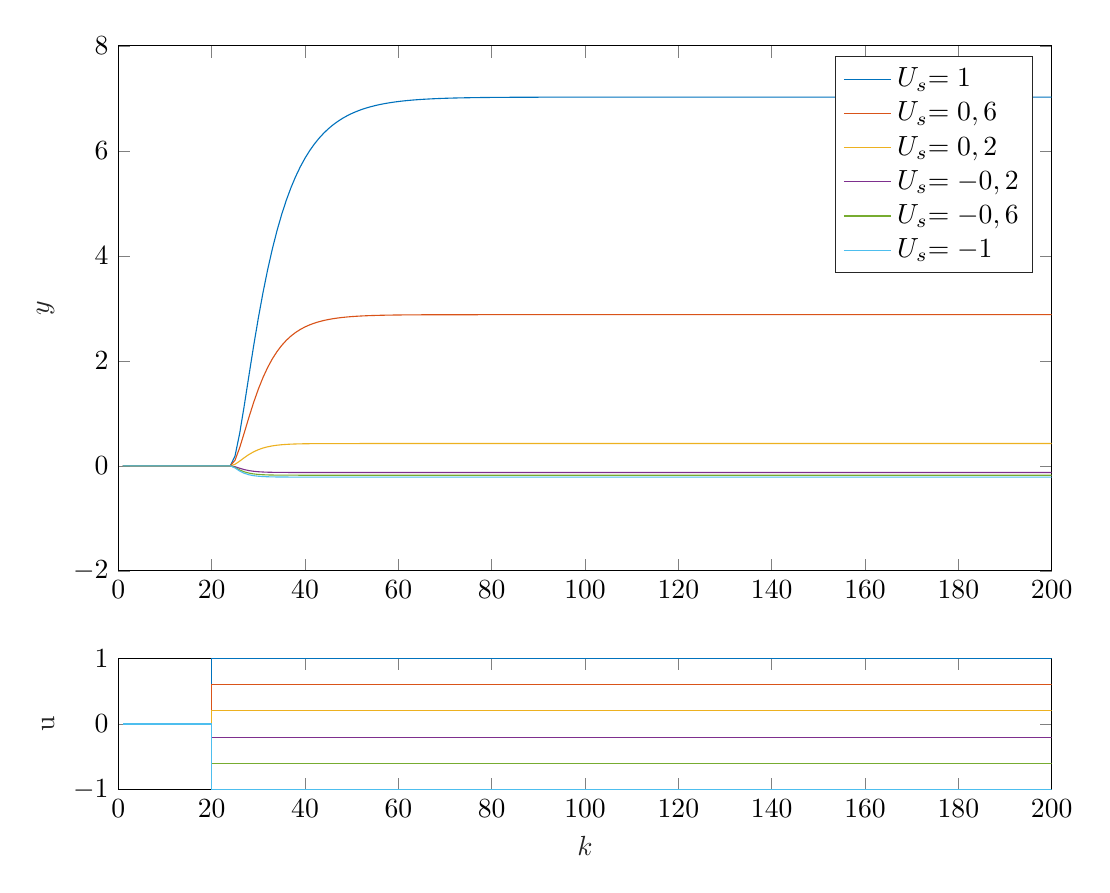
\begin{tikzpicture}

\begin{axis}[%
width=4.667in,
height=0.656in,
at={(0.583in,0.525in)},
scale only axis,
xmin=0,
xmax=200,
xtick={0,20,40,60,80,100,120,140,160,180,200},
xlabel style={font=\color{white!15!black}},
xlabel={$k$},
ymin=-1,
ymax=1,
ytick={-1,0,1},
ylabel style={font=\color{white!15!black}},
ylabel={u},
axis background/.style={fill=white}
]
\addplot[const plot, color=mycolor1, forget plot] table[row sep=crcr] {%
1	0\\
2	0\\
3	0\\
4	0\\
5	0\\
6	0\\
7	0\\
8	0\\
9	0\\
10	0\\
11	0\\
12	0\\
13	0\\
14	0\\
15	0\\
16	0\\
17	0\\
18	0\\
19	0\\
20	1\\
21	1\\
22	1\\
23	1\\
24	1\\
25	1\\
26	1\\
27	1\\
28	1\\
29	1\\
30	1\\
31	1\\
32	1\\
33	1\\
34	1\\
35	1\\
36	1\\
37	1\\
38	1\\
39	1\\
40	1\\
41	1\\
42	1\\
43	1\\
44	1\\
45	1\\
46	1\\
47	1\\
48	1\\
49	1\\
50	1\\
51	1\\
52	1\\
53	1\\
54	1\\
55	1\\
56	1\\
57	1\\
58	1\\
59	1\\
60	1\\
61	1\\
62	1\\
63	1\\
64	1\\
65	1\\
66	1\\
67	1\\
68	1\\
69	1\\
70	1\\
71	1\\
72	1\\
73	1\\
74	1\\
75	1\\
76	1\\
77	1\\
78	1\\
79	1\\
80	1\\
81	1\\
82	1\\
83	1\\
84	1\\
85	1\\
86	1\\
87	1\\
88	1\\
89	1\\
90	1\\
91	1\\
92	1\\
93	1\\
94	1\\
95	1\\
96	1\\
97	1\\
98	1\\
99	1\\
100	1\\
101	1\\
102	1\\
103	1\\
104	1\\
105	1\\
106	1\\
107	1\\
108	1\\
109	1\\
110	1\\
111	1\\
112	1\\
113	1\\
114	1\\
115	1\\
116	1\\
117	1\\
118	1\\
119	1\\
120	1\\
121	1\\
122	1\\
123	1\\
124	1\\
125	1\\
126	1\\
127	1\\
128	1\\
129	1\\
130	1\\
131	1\\
132	1\\
133	1\\
134	1\\
135	1\\
136	1\\
137	1\\
138	1\\
139	1\\
140	1\\
141	1\\
142	1\\
143	1\\
144	1\\
145	1\\
146	1\\
147	1\\
148	1\\
149	1\\
150	1\\
151	1\\
152	1\\
153	1\\
154	1\\
155	1\\
156	1\\
157	1\\
158	1\\
159	1\\
160	1\\
161	1\\
162	1\\
163	1\\
164	1\\
165	1\\
166	1\\
167	1\\
168	1\\
169	1\\
170	1\\
171	1\\
172	1\\
173	1\\
174	1\\
175	1\\
176	1\\
177	1\\
178	1\\
179	1\\
180	1\\
181	1\\
182	1\\
183	1\\
184	1\\
185	1\\
186	1\\
187	1\\
188	1\\
189	1\\
190	1\\
191	1\\
192	1\\
193	1\\
194	1\\
195	1\\
196	1\\
197	1\\
198	1\\
199	1\\
200	1\\
};
\addplot[const plot, color=mycolor2, forget plot] table[row sep=crcr] {%
1	0\\
2	0\\
3	0\\
4	0\\
5	0\\
6	0\\
7	0\\
8	0\\
9	0\\
10	0\\
11	0\\
12	0\\
13	0\\
14	0\\
15	0\\
16	0\\
17	0\\
18	0\\
19	0\\
20	0.6\\
21	0.6\\
22	0.6\\
23	0.6\\
24	0.6\\
25	0.6\\
26	0.6\\
27	0.6\\
28	0.6\\
29	0.6\\
30	0.6\\
31	0.6\\
32	0.6\\
33	0.6\\
34	0.6\\
35	0.6\\
36	0.6\\
37	0.6\\
38	0.6\\
39	0.6\\
40	0.6\\
41	0.6\\
42	0.6\\
43	0.6\\
44	0.6\\
45	0.6\\
46	0.6\\
47	0.6\\
48	0.6\\
49	0.6\\
50	0.6\\
51	0.6\\
52	0.6\\
53	0.6\\
54	0.6\\
55	0.6\\
56	0.6\\
57	0.6\\
58	0.6\\
59	0.6\\
60	0.6\\
61	0.6\\
62	0.6\\
63	0.6\\
64	0.6\\
65	0.6\\
66	0.6\\
67	0.6\\
68	0.6\\
69	0.6\\
70	0.6\\
71	0.6\\
72	0.6\\
73	0.6\\
74	0.6\\
75	0.6\\
76	0.6\\
77	0.6\\
78	0.6\\
79	0.6\\
80	0.6\\
81	0.6\\
82	0.6\\
83	0.6\\
84	0.6\\
85	0.6\\
86	0.6\\
87	0.6\\
88	0.6\\
89	0.6\\
90	0.6\\
91	0.6\\
92	0.6\\
93	0.6\\
94	0.6\\
95	0.6\\
96	0.6\\
97	0.6\\
98	0.6\\
99	0.6\\
100	0.6\\
101	0.6\\
102	0.6\\
103	0.6\\
104	0.6\\
105	0.6\\
106	0.6\\
107	0.6\\
108	0.6\\
109	0.6\\
110	0.6\\
111	0.6\\
112	0.6\\
113	0.6\\
114	0.6\\
115	0.6\\
116	0.6\\
117	0.6\\
118	0.6\\
119	0.6\\
120	0.6\\
121	0.6\\
122	0.6\\
123	0.6\\
124	0.6\\
125	0.6\\
126	0.6\\
127	0.6\\
128	0.6\\
129	0.6\\
130	0.6\\
131	0.6\\
132	0.6\\
133	0.6\\
134	0.6\\
135	0.6\\
136	0.6\\
137	0.6\\
138	0.6\\
139	0.6\\
140	0.6\\
141	0.6\\
142	0.6\\
143	0.6\\
144	0.6\\
145	0.6\\
146	0.6\\
147	0.6\\
148	0.6\\
149	0.6\\
150	0.6\\
151	0.6\\
152	0.6\\
153	0.6\\
154	0.6\\
155	0.6\\
156	0.6\\
157	0.6\\
158	0.6\\
159	0.6\\
160	0.6\\
161	0.6\\
162	0.6\\
163	0.6\\
164	0.6\\
165	0.6\\
166	0.6\\
167	0.6\\
168	0.6\\
169	0.6\\
170	0.6\\
171	0.6\\
172	0.6\\
173	0.6\\
174	0.6\\
175	0.6\\
176	0.6\\
177	0.6\\
178	0.6\\
179	0.6\\
180	0.6\\
181	0.6\\
182	0.6\\
183	0.6\\
184	0.6\\
185	0.6\\
186	0.6\\
187	0.6\\
188	0.6\\
189	0.6\\
190	0.6\\
191	0.6\\
192	0.6\\
193	0.6\\
194	0.6\\
195	0.6\\
196	0.6\\
197	0.6\\
198	0.6\\
199	0.6\\
200	0.6\\
};
\addplot[const plot, color=mycolor3, forget plot] table[row sep=crcr] {%
1	0\\
2	0\\
3	0\\
4	0\\
5	0\\
6	0\\
7	0\\
8	0\\
9	0\\
10	0\\
11	0\\
12	0\\
13	0\\
14	0\\
15	0\\
16	0\\
17	0\\
18	0\\
19	0\\
20	0.2\\
21	0.2\\
22	0.2\\
23	0.2\\
24	0.2\\
25	0.2\\
26	0.2\\
27	0.2\\
28	0.2\\
29	0.2\\
30	0.2\\
31	0.2\\
32	0.2\\
33	0.2\\
34	0.2\\
35	0.2\\
36	0.2\\
37	0.2\\
38	0.2\\
39	0.2\\
40	0.2\\
41	0.2\\
42	0.2\\
43	0.2\\
44	0.2\\
45	0.2\\
46	0.2\\
47	0.2\\
48	0.2\\
49	0.2\\
50	0.2\\
51	0.2\\
52	0.2\\
53	0.2\\
54	0.2\\
55	0.2\\
56	0.2\\
57	0.2\\
58	0.2\\
59	0.2\\
60	0.2\\
61	0.2\\
62	0.2\\
63	0.2\\
64	0.2\\
65	0.2\\
66	0.2\\
67	0.2\\
68	0.2\\
69	0.2\\
70	0.2\\
71	0.2\\
72	0.2\\
73	0.2\\
74	0.2\\
75	0.2\\
76	0.2\\
77	0.2\\
78	0.2\\
79	0.2\\
80	0.2\\
81	0.2\\
82	0.2\\
83	0.2\\
84	0.2\\
85	0.2\\
86	0.2\\
87	0.2\\
88	0.2\\
89	0.2\\
90	0.2\\
91	0.2\\
92	0.2\\
93	0.2\\
94	0.2\\
95	0.2\\
96	0.2\\
97	0.2\\
98	0.2\\
99	0.2\\
100	0.2\\
101	0.2\\
102	0.2\\
103	0.2\\
104	0.2\\
105	0.2\\
106	0.2\\
107	0.2\\
108	0.2\\
109	0.2\\
110	0.2\\
111	0.2\\
112	0.2\\
113	0.2\\
114	0.2\\
115	0.2\\
116	0.2\\
117	0.2\\
118	0.2\\
119	0.2\\
120	0.2\\
121	0.2\\
122	0.2\\
123	0.2\\
124	0.2\\
125	0.2\\
126	0.2\\
127	0.2\\
128	0.2\\
129	0.2\\
130	0.2\\
131	0.2\\
132	0.2\\
133	0.2\\
134	0.2\\
135	0.2\\
136	0.2\\
137	0.2\\
138	0.2\\
139	0.2\\
140	0.2\\
141	0.2\\
142	0.2\\
143	0.2\\
144	0.2\\
145	0.2\\
146	0.2\\
147	0.2\\
148	0.2\\
149	0.2\\
150	0.2\\
151	0.2\\
152	0.2\\
153	0.2\\
154	0.2\\
155	0.2\\
156	0.2\\
157	0.2\\
158	0.2\\
159	0.2\\
160	0.2\\
161	0.2\\
162	0.2\\
163	0.2\\
164	0.2\\
165	0.2\\
166	0.2\\
167	0.2\\
168	0.2\\
169	0.2\\
170	0.2\\
171	0.2\\
172	0.2\\
173	0.2\\
174	0.2\\
175	0.2\\
176	0.2\\
177	0.2\\
178	0.2\\
179	0.2\\
180	0.2\\
181	0.2\\
182	0.2\\
183	0.2\\
184	0.2\\
185	0.2\\
186	0.2\\
187	0.2\\
188	0.2\\
189	0.2\\
190	0.2\\
191	0.2\\
192	0.2\\
193	0.2\\
194	0.2\\
195	0.2\\
196	0.2\\
197	0.2\\
198	0.2\\
199	0.2\\
200	0.2\\
};
\addplot[const plot, color=mycolor4, forget plot] table[row sep=crcr] {%
1	0\\
2	0\\
3	0\\
4	0\\
5	0\\
6	0\\
7	0\\
8	0\\
9	0\\
10	0\\
11	0\\
12	0\\
13	0\\
14	0\\
15	0\\
16	0\\
17	0\\
18	0\\
19	0\\
20	-0.2\\
21	-0.2\\
22	-0.2\\
23	-0.2\\
24	-0.2\\
25	-0.2\\
26	-0.2\\
27	-0.2\\
28	-0.2\\
29	-0.2\\
30	-0.2\\
31	-0.2\\
32	-0.2\\
33	-0.2\\
34	-0.2\\
35	-0.2\\
36	-0.2\\
37	-0.2\\
38	-0.2\\
39	-0.2\\
40	-0.2\\
41	-0.2\\
42	-0.2\\
43	-0.2\\
44	-0.2\\
45	-0.2\\
46	-0.2\\
47	-0.2\\
48	-0.2\\
49	-0.2\\
50	-0.2\\
51	-0.2\\
52	-0.2\\
53	-0.2\\
54	-0.2\\
55	-0.2\\
56	-0.2\\
57	-0.2\\
58	-0.2\\
59	-0.2\\
60	-0.2\\
61	-0.2\\
62	-0.2\\
63	-0.2\\
64	-0.2\\
65	-0.2\\
66	-0.2\\
67	-0.2\\
68	-0.2\\
69	-0.2\\
70	-0.2\\
71	-0.2\\
72	-0.2\\
73	-0.2\\
74	-0.2\\
75	-0.2\\
76	-0.2\\
77	-0.2\\
78	-0.2\\
79	-0.2\\
80	-0.2\\
81	-0.2\\
82	-0.2\\
83	-0.2\\
84	-0.2\\
85	-0.2\\
86	-0.2\\
87	-0.2\\
88	-0.2\\
89	-0.2\\
90	-0.2\\
91	-0.2\\
92	-0.2\\
93	-0.2\\
94	-0.2\\
95	-0.2\\
96	-0.2\\
97	-0.2\\
98	-0.2\\
99	-0.2\\
100	-0.2\\
101	-0.2\\
102	-0.2\\
103	-0.2\\
104	-0.2\\
105	-0.2\\
106	-0.2\\
107	-0.2\\
108	-0.2\\
109	-0.2\\
110	-0.2\\
111	-0.2\\
112	-0.2\\
113	-0.2\\
114	-0.2\\
115	-0.2\\
116	-0.2\\
117	-0.2\\
118	-0.2\\
119	-0.2\\
120	-0.2\\
121	-0.2\\
122	-0.2\\
123	-0.2\\
124	-0.2\\
125	-0.2\\
126	-0.2\\
127	-0.2\\
128	-0.2\\
129	-0.2\\
130	-0.2\\
131	-0.2\\
132	-0.2\\
133	-0.2\\
134	-0.2\\
135	-0.2\\
136	-0.2\\
137	-0.2\\
138	-0.2\\
139	-0.2\\
140	-0.2\\
141	-0.2\\
142	-0.2\\
143	-0.2\\
144	-0.2\\
145	-0.2\\
146	-0.2\\
147	-0.2\\
148	-0.2\\
149	-0.2\\
150	-0.2\\
151	-0.2\\
152	-0.2\\
153	-0.2\\
154	-0.2\\
155	-0.2\\
156	-0.2\\
157	-0.2\\
158	-0.2\\
159	-0.2\\
160	-0.2\\
161	-0.2\\
162	-0.2\\
163	-0.2\\
164	-0.2\\
165	-0.2\\
166	-0.2\\
167	-0.2\\
168	-0.2\\
169	-0.2\\
170	-0.2\\
171	-0.2\\
172	-0.2\\
173	-0.2\\
174	-0.2\\
175	-0.2\\
176	-0.2\\
177	-0.2\\
178	-0.2\\
179	-0.2\\
180	-0.2\\
181	-0.2\\
182	-0.2\\
183	-0.2\\
184	-0.2\\
185	-0.2\\
186	-0.2\\
187	-0.2\\
188	-0.2\\
189	-0.2\\
190	-0.2\\
191	-0.2\\
192	-0.2\\
193	-0.2\\
194	-0.2\\
195	-0.2\\
196	-0.2\\
197	-0.2\\
198	-0.2\\
199	-0.2\\
200	-0.2\\
};
\addplot[const plot, color=mycolor5, forget plot] table[row sep=crcr] {%
1	0\\
2	0\\
3	0\\
4	0\\
5	0\\
6	0\\
7	0\\
8	0\\
9	0\\
10	0\\
11	0\\
12	0\\
13	0\\
14	0\\
15	0\\
16	0\\
17	0\\
18	0\\
19	0\\
20	-0.6\\
21	-0.6\\
22	-0.6\\
23	-0.6\\
24	-0.6\\
25	-0.6\\
26	-0.6\\
27	-0.6\\
28	-0.6\\
29	-0.6\\
30	-0.6\\
31	-0.6\\
32	-0.6\\
33	-0.6\\
34	-0.6\\
35	-0.6\\
36	-0.6\\
37	-0.6\\
38	-0.6\\
39	-0.6\\
40	-0.6\\
41	-0.6\\
42	-0.6\\
43	-0.6\\
44	-0.6\\
45	-0.6\\
46	-0.6\\
47	-0.6\\
48	-0.6\\
49	-0.6\\
50	-0.6\\
51	-0.6\\
52	-0.6\\
53	-0.6\\
54	-0.6\\
55	-0.6\\
56	-0.6\\
57	-0.6\\
58	-0.6\\
59	-0.6\\
60	-0.6\\
61	-0.6\\
62	-0.6\\
63	-0.6\\
64	-0.6\\
65	-0.6\\
66	-0.6\\
67	-0.6\\
68	-0.6\\
69	-0.6\\
70	-0.6\\
71	-0.6\\
72	-0.6\\
73	-0.6\\
74	-0.6\\
75	-0.6\\
76	-0.6\\
77	-0.6\\
78	-0.6\\
79	-0.6\\
80	-0.6\\
81	-0.6\\
82	-0.6\\
83	-0.6\\
84	-0.6\\
85	-0.6\\
86	-0.6\\
87	-0.6\\
88	-0.6\\
89	-0.6\\
90	-0.6\\
91	-0.6\\
92	-0.6\\
93	-0.6\\
94	-0.6\\
95	-0.6\\
96	-0.6\\
97	-0.6\\
98	-0.6\\
99	-0.6\\
100	-0.6\\
101	-0.6\\
102	-0.6\\
103	-0.6\\
104	-0.6\\
105	-0.6\\
106	-0.6\\
107	-0.6\\
108	-0.6\\
109	-0.6\\
110	-0.6\\
111	-0.6\\
112	-0.6\\
113	-0.6\\
114	-0.6\\
115	-0.6\\
116	-0.6\\
117	-0.6\\
118	-0.6\\
119	-0.6\\
120	-0.6\\
121	-0.6\\
122	-0.6\\
123	-0.6\\
124	-0.6\\
125	-0.6\\
126	-0.6\\
127	-0.6\\
128	-0.6\\
129	-0.6\\
130	-0.6\\
131	-0.6\\
132	-0.6\\
133	-0.6\\
134	-0.6\\
135	-0.6\\
136	-0.6\\
137	-0.6\\
138	-0.6\\
139	-0.6\\
140	-0.6\\
141	-0.6\\
142	-0.6\\
143	-0.6\\
144	-0.6\\
145	-0.6\\
146	-0.6\\
147	-0.6\\
148	-0.6\\
149	-0.6\\
150	-0.6\\
151	-0.6\\
152	-0.6\\
153	-0.6\\
154	-0.6\\
155	-0.6\\
156	-0.6\\
157	-0.6\\
158	-0.6\\
159	-0.6\\
160	-0.6\\
161	-0.6\\
162	-0.6\\
163	-0.6\\
164	-0.6\\
165	-0.6\\
166	-0.6\\
167	-0.6\\
168	-0.6\\
169	-0.6\\
170	-0.6\\
171	-0.6\\
172	-0.6\\
173	-0.6\\
174	-0.6\\
175	-0.6\\
176	-0.6\\
177	-0.6\\
178	-0.6\\
179	-0.6\\
180	-0.6\\
181	-0.6\\
182	-0.6\\
183	-0.6\\
184	-0.6\\
185	-0.6\\
186	-0.6\\
187	-0.6\\
188	-0.6\\
189	-0.6\\
190	-0.6\\
191	-0.6\\
192	-0.6\\
193	-0.6\\
194	-0.6\\
195	-0.6\\
196	-0.6\\
197	-0.6\\
198	-0.6\\
199	-0.6\\
200	-0.6\\
};
\addplot[const plot, color=mycolor6, forget plot] table[row sep=crcr] {%
1	0\\
2	0\\
3	0\\
4	0\\
5	0\\
6	0\\
7	0\\
8	0\\
9	0\\
10	0\\
11	0\\
12	0\\
13	0\\
14	0\\
15	0\\
16	0\\
17	0\\
18	0\\
19	0\\
20	-1\\
21	-1\\
22	-1\\
23	-1\\
24	-1\\
25	-1\\
26	-1\\
27	-1\\
28	-1\\
29	-1\\
30	-1\\
31	-1\\
32	-1\\
33	-1\\
34	-1\\
35	-1\\
36	-1\\
37	-1\\
38	-1\\
39	-1\\
40	-1\\
41	-1\\
42	-1\\
43	-1\\
44	-1\\
45	-1\\
46	-1\\
47	-1\\
48	-1\\
49	-1\\
50	-1\\
51	-1\\
52	-1\\
53	-1\\
54	-1\\
55	-1\\
56	-1\\
57	-1\\
58	-1\\
59	-1\\
60	-1\\
61	-1\\
62	-1\\
63	-1\\
64	-1\\
65	-1\\
66	-1\\
67	-1\\
68	-1\\
69	-1\\
70	-1\\
71	-1\\
72	-1\\
73	-1\\
74	-1\\
75	-1\\
76	-1\\
77	-1\\
78	-1\\
79	-1\\
80	-1\\
81	-1\\
82	-1\\
83	-1\\
84	-1\\
85	-1\\
86	-1\\
87	-1\\
88	-1\\
89	-1\\
90	-1\\
91	-1\\
92	-1\\
93	-1\\
94	-1\\
95	-1\\
96	-1\\
97	-1\\
98	-1\\
99	-1\\
100	-1\\
101	-1\\
102	-1\\
103	-1\\
104	-1\\
105	-1\\
106	-1\\
107	-1\\
108	-1\\
109	-1\\
110	-1\\
111	-1\\
112	-1\\
113	-1\\
114	-1\\
115	-1\\
116	-1\\
117	-1\\
118	-1\\
119	-1\\
120	-1\\
121	-1\\
122	-1\\
123	-1\\
124	-1\\
125	-1\\
126	-1\\
127	-1\\
128	-1\\
129	-1\\
130	-1\\
131	-1\\
132	-1\\
133	-1\\
134	-1\\
135	-1\\
136	-1\\
137	-1\\
138	-1\\
139	-1\\
140	-1\\
141	-1\\
142	-1\\
143	-1\\
144	-1\\
145	-1\\
146	-1\\
147	-1\\
148	-1\\
149	-1\\
150	-1\\
151	-1\\
152	-1\\
153	-1\\
154	-1\\
155	-1\\
156	-1\\
157	-1\\
158	-1\\
159	-1\\
160	-1\\
161	-1\\
162	-1\\
163	-1\\
164	-1\\
165	-1\\
166	-1\\
167	-1\\
168	-1\\
169	-1\\
170	-1\\
171	-1\\
172	-1\\
173	-1\\
174	-1\\
175	-1\\
176	-1\\
177	-1\\
178	-1\\
179	-1\\
180	-1\\
181	-1\\
182	-1\\
183	-1\\
184	-1\\
185	-1\\
186	-1\\
187	-1\\
188	-1\\
189	-1\\
190	-1\\
191	-1\\
192	-1\\
193	-1\\
194	-1\\
195	-1\\
196	-1\\
197	-1\\
198	-1\\
199	-1\\
200	-1\\
};
\end{axis}

\begin{axis}[%
width=4.667in,
height=2.625in,
at={(0.583in,1.619in)},
scale only axis,
xmin=0,
xmax=200,
xtick={0,20,40,60,80,100,120,140,160,180,200},
ymin=-2,
ymax=8,
ytick={-2,0,2,4,6,8},
ylabel style={font=\color{white!15!black}},
ylabel={$y$},
axis background/.style={fill=white},
legend style={legend cell align=left, align=left, draw=white!15!black}
]
\addplot [color=mycolor1]
  table[row sep=crcr]{%
1	0\\
2	0\\
3	0\\
4	0\\
5	0\\
6	0\\
7	0\\
8	0\\
9	0\\
10	0\\
11	0\\
12	0\\
13	0\\
14	0\\
15	0\\
16	0\\
17	0\\
18	0\\
19	0\\
20	0\\
21	0\\
22	0\\
23	0\\
24	0\\
25	0.187021166666667\\
26	0.6177121086775\\
27	1.15713812513778\\
28	1.72826134563714\\
29	2.28857090407221\\
30	2.81598000810106\\
31	3.30033523448568\\
32	3.73832226743667\\
33	4.13042497668062\\
34	4.47912397208548\\
35	4.78784169917674\\
36	5.06033571970525\\
37	5.30035977120632\\
38	5.51148367608905\\
39	5.6970064658836\\
40	5.85992329434167\\
41	6.00292256301261\\
42	6.12839925555669\\
43	6.23847624709673\\
44	6.33502882283716\\
45	6.41970971562484\\
46	6.49397320637228\\
47	6.55909755828853\\
48	6.61620547787984\\
49	6.6662825350215\\
50	6.71019360498331\\
51	6.74869746169737\\
52	6.7824596806132\\
53	6.81206401726699\\
54	6.83802242378144\\
55	6.86078385557317\\
56	6.88074200787935\\
57	6.89824210821422\\
58	6.91358687757493\\
59	6.92704176068014\\
60	6.9388395139979\\
61	6.94918422988833\\
62	6.95825486584292\\
63	6.96620833949031\\
64	6.97318224267801\\
65	6.97929722144122\\
66	6.98465906294563\\
67	6.98936052545592\\
68	6.99348294295602\\
69	6.99709763216175\\
70	7.00026712625508\\
71	7.00304625667623\\
72	7.00548310168414\\
73	7.00761981809253\\
74	7.00949337056883\\
75	7.01113617111165\\
76	7.01257663976922\\
77	7.01383969629842\\
78	7.01494719127006\\
79	7.01591828407818\\
80	7.01676977439269\\
81	7.01751639278953\\
82	7.01817105558595\\
83	7.01874508828967\\
84	7.01924842152737\\
85	7.01968976284209\\
86	7.02007674733167\\
87	7.02041606973404\\
88	7.02071360024454\\
89	7.02097448606895\\
90	7.02120324046883\\
91	7.02140382083989\\
92	7.02157969717396\\
93	7.02173391208904\\
94	7.02186913346578\\
95	7.02198770060126\\
96	7.02209166467821\\
97	7.02218282424996\\
98	7.02226275635504\\
99	7.0223328437995\\
100	7.02239429907915\\
101	7.02244818535545\\
102	7.02249543484792\\
103	7.02253686496133\\
104	7.02257319242663\\
105	7.02260504570015\\
106	7.02263297583581\\
107	7.0226574660182\\
108	7.02267893992153\\
109	7.02269776903914\\
110	7.0227142791102\\
111	7.02272875575494\\
112	7.0227414494158\\
113	7.02275257969005\\
114	7.02276233912873\\
115	7.02277089656777\\
116	7.02277840004879\\
117	7.0227849793802\\
118	7.02279074838283\\
119	7.02279580685903\\
120	7.02280024231922\\
121	7.02280413149578\\
122	7.02280754167053\\
123	7.02281053183866\\
124	7.02281315372936\\
125	7.0228154527007\\
126	7.02281746852433\\
127	7.02281923607351\\
128	7.02282078592641\\
129	7.02282214489511\\
130	7.02282333648944\\
131	7.0228243813237\\
132	7.02282529747326\\
133	7.02282610078729\\
134	7.02282680516292\\
135	7.02282742278569\\
136	7.02282796434033\\
137	7.02282843919558\\
138	7.02282885556634\\
139	7.02282922065572\\
140	7.02282954077968\\
141	7.02282982147627\\
142	7.02283006760149\\
143	7.02283028341325\\
144	7.02283047264503\\
145	7.02283063857049\\
146	7.02283078406011\\
147	7.02283091163083\\
148	7.02283102348958\\
149	7.0228311215715\\
150	7.02283120757337\\
151	7.02283128298301\\
152	7.022831349105\\
153	7.02283140708321\\
154	7.02283145792067\\
155	7.02283150249684\\
156	7.02283154158289\\
157	7.02283157585499\\
158	7.02283160590605\\
159	7.02283163225593\\
160	7.02283165536049\\
161	7.02283167561942\\
162	7.02283169338321\\
163	7.02283170895916\\
164	7.02283172261674\\
165	7.0228317345922\\
166	7.02283174509274\\
167	7.0228317543\\
168	7.02283176237327\\
169	7.02283176945221\\
170	7.02283177565929\\
171	7.02283178110189\\
172	7.02283178587416\\
173	7.02283179005867\\
174	7.0228317937278\\
175	7.02283179694503\\
176	7.02283179976602\\
177	7.02283180223957\\
178	7.02283180440847\\
179	7.02283180631024\\
180	7.02283180797778\\
181	7.02283180943994\\
182	7.02283181072202\\
183	7.0228318118462\\
184	7.02283181283192\\
185	7.02283181369623\\
186	7.0228318144541\\
187	7.02283181511862\\
188	7.0228318157013\\
189	7.02283181621221\\
190	7.0228318166602\\
191	7.02283181705302\\
192	7.02283181739745\\
193	7.02283181769946\\
194	7.02283181796428\\
195	7.02283181819648\\
196	7.02283181840008\\
197	7.02283181857861\\
198	7.02283181873515\\
199	7.0228318188724\\
200	7.02283181899276\\
};
\addlegendentry{$\text{U}_\text{s}\text{=1}$}

\addplot [color=mycolor2]
  table[row sep=crcr]{%
1	0\\
2	0\\
3	0\\
4	0\\
5	0\\
6	0\\
7	0\\
8	0\\
9	0\\
10	0\\
11	0\\
12	0\\
13	0\\
14	0\\
15	0\\
16	0\\
17	0\\
18	0\\
19	0\\
20	0\\
21	0\\
22	0\\
23	0\\
24	0\\
25	0.105917718127564\\
26	0.344464751567524\\
27	0.633871289498794\\
28	0.929560401059789\\
29	1.20866320827921\\
30	1.46077065672109\\
31	1.68244380434273\\
32	1.87398360482631\\
33	2.03755434641196\\
34	2.17611414365154\\
35	2.29282330310435\\
36	2.39073286714509\\
37	2.47263506073569\\
38	2.54100526286437\\
39	2.59799394637634\\
40	2.64544432059064\\
41	2.68492173959127\\
42	2.71774707149373\\
43	2.74502983361949\\
44	2.76769899655006\\
45	2.78653055668825\\
46	2.80217163973708\\
47	2.81516124715862\\
48	2.82594792627675\\
49	2.83490471085001\\
50	2.84234168909482\\
51	2.84851653740868\\
52	2.85364332601709\\
53	2.85789986618548\\
54	2.86143383220428\\
55	2.86436785742963\\
56	2.86680377326701\\
57	2.86882613339667\\
58	2.87050514264485\\
59	2.87189909039995\\
60	2.87305637197655\\
61	2.87401716745229\\
62	2.87481483586965\\
63	2.87547707296932\\
64	2.87602687250688\\
65	2.87648332444254\\
66	2.87686227766481\\
67	2.87717689022666\\
68	2.8774380861797\\
69	2.87765493485673\\
70	2.87783496576499\\
71	2.87798443001964\\
72	2.87810851739221\\
73	2.87821153650904\\
74	2.8782970644556\\
75	2.87836807098077\\
76	2.87842702161332\\
77	2.87847596327094\\
78	2.87851659533427\\
79	2.87855032865352\\
80	2.87857833453681\\
81	2.87860158542093\\
82	2.87862088863682\\
83	2.87863691444216\\
84	2.87865021929448\\
85	2.87866126517276\\
86	2.87867043561854\\
87	2.87867804905349\\
88	2.87868436983584\\
89	2.87868961743955\\
90	2.87869397407503\\
91	2.87869759101597\\
92	2.87870059385196\\
93	2.87870308684924\\
94	2.87870515657117\\
95	2.87870687488384\\
96	2.87870830145154\\
97	2.8787094858084\\
98	2.87871046907837\\
99	2.87871128540313\\
100	2.87871196312759\\
101	2.87871252578411\\
102	2.87871299290959\\
103	2.87871338072382\\
104	2.87871370269273\\
105	2.87871396999591\\
106	2.87871419191483\\
107	2.87871437615508\\
108	2.87871452911397\\
109	2.87871465610262\\
110	2.87871476153041\\
111	2.87871484905806\\
112	2.87871492172477\\
113	2.87871498205371\\
114	2.87871503213965\\
115	2.87871507372172\\
116	2.87871510824374\\
117	2.87871513690442\\
118	2.87871516069893\\
119	2.87871518045346\\
120	2.87871519685396\\
121	2.87871521046989\\
122	2.87871522177403\\
123	2.87871523115888\\
124	2.87871523895033\\
125	2.87871524541889\\
126	2.87871525078919\\
127	2.87871525524768\\
128	2.87871525894919\\
129	2.87871526202223\\
130	2.87871526457352\\
131	2.87871526669163\\
132	2.87871526845012\\
133	2.87871526991004\\
134	2.87871527112209\\
135	2.87871527212835\\
136	2.87871527296376\\
137	2.87871527365733\\
138	2.87871527423314\\
139	2.87871527471119\\
140	2.87871527510807\\
141	2.87871527543756\\
142	2.87871527571112\\
143	2.87871527593823\\
144	2.87871527612677\\
145	2.87871527628331\\
146	2.87871527641326\\
147	2.87871527652116\\
148	2.87871527661073\\
149	2.8787152766851\\
150	2.87871527674684\\
151	2.8787152767981\\
152	2.87871527684065\\
153	2.87871527687598\\
154	2.87871527690531\\
155	2.87871527692966\\
156	2.87871527694988\\
157	2.87871527696666\\
158	2.8787152769806\\
159	2.87871527699216\\
160	2.87871527700177\\
161	2.87871527700974\\
162	2.87871527701636\\
163	2.87871527702186\\
164	2.87871527702642\\
165	2.87871527703021\\
166	2.87871527703335\\
167	2.87871527703596\\
168	2.87871527703813\\
169	2.87871527703993\\
170	2.87871527704142\\
171	2.87871527704266\\
172	2.87871527704369\\
173	2.87871527704455\\
174	2.87871527704526\\
175	2.87871527704585\\
176	2.87871527704634\\
177	2.87871527704674\\
178	2.87871527704708\\
179	2.87871527704736\\
180	2.87871527704759\\
181	2.87871527704779\\
182	2.87871527704795\\
183	2.87871527704808\\
184	2.87871527704819\\
185	2.87871527704828\\
186	2.87871527704836\\
187	2.87871527704842\\
188	2.87871527704847\\
189	2.87871527704852\\
190	2.87871527704855\\
191	2.87871527704858\\
192	2.87871527704861\\
193	2.87871527704863\\
194	2.87871527704865\\
195	2.87871527704866\\
196	2.87871527704867\\
197	2.87871527704868\\
198	2.87871527704869\\
199	2.8787152770487\\
200	2.8787152770487\\
};
\addlegendentry{$\text{U}_\text{s}\text{=0,6}$}

\addplot [color=mycolor3]
  table[row sep=crcr]{%
1	0\\
2	0\\
3	0\\
4	0\\
5	0\\
6	0\\
7	0\\
8	0\\
9	0\\
10	0\\
11	0\\
12	0\\
13	0\\
14	0\\
15	0\\
16	0\\
17	0\\
18	0\\
19	0\\
20	0\\
21	0\\
22	0\\
23	0\\
24	0\\
25	0.0289156588865096\\
26	0.0894682048721172\\
27	0.155802404989047\\
28	0.216414639654754\\
29	0.267203961578747\\
30	0.307662999632864\\
31	0.338846921882816\\
32	0.362333838529911\\
33	0.379726634117973\\
34	0.392441944939566\\
35	0.401644900606398\\
36	0.408252725719196\\
37	0.412966648751595\\
38	0.41631171556038\\
39	0.418675019991484\\
40	0.420338584697667\\
41	0.421505975645158\\
42	0.42232303621694\\
43	0.422893623251372\\
44	0.423291326396279\\
45	0.423568073143304\\
46	0.423760378244908\\
47	0.4238938431838\\
48	0.423986373189291\\
49	0.424050464269623\\
50	0.424094821476588\\
51	0.424125499483137\\
52	0.424146703837411\\
53	0.424161352277196\\
54	0.424171467025686\\
55	0.424178448407745\\
56	0.4241832653591\\
57	0.424186587872796\\
58	0.424188878960224\\
59	0.424190458430664\\
60	0.424191547082653\\
61	0.424192297297316\\
62	0.424192814202322\\
63	0.424193170303356\\
64	0.424193415593771\\
65	0.424193584536459\\
66	0.424193700883544\\
67	0.424193781002268\\
68	0.424193836169277\\
69	0.42419387415284\\
70	0.42419390030372\\
71	0.42419391830711\\
72	0.424193930700849\\
73	0.424193939232497\\
74	0.424193945105334\\
75	0.424193949147828\\
76	0.424193951930352\\
77	0.424193953845568\\
78	0.424193955163786\\
79	0.424193956071081\\
80	0.424193956695538\\
81	0.424193957125322\\
82	0.424193957421119\\
83	0.424193957624696\\
84	0.424193957764804\\
85	0.424193957861229\\
86	0.424193957927591\\
87	0.424193957973262\\
88	0.424193958004693\\
89	0.424193958026324\\
90	0.42419395804121\\
91	0.424193958051455\\
92	0.424193958058506\\
93	0.424193958063358\\
94	0.424193958066697\\
95	0.424193958068995\\
96	0.424193958070577\\
97	0.424193958071665\\
98	0.424193958072414\\
99	0.424193958072929\\
100	0.424193958073284\\
101	0.424193958073528\\
102	0.424193958073696\\
103	0.424193958073812\\
104	0.424193958073891\\
105	0.424193958073946\\
106	0.424193958073984\\
107	0.42419395807401\\
108	0.424193958074027\\
109	0.42419395807404\\
110	0.424193958074048\\
111	0.424193958074054\\
112	0.424193958074058\\
113	0.424193958074061\\
114	0.424193958074063\\
115	0.424193958074064\\
116	0.424193958074065\\
117	0.424193958074065\\
118	0.424193958074066\\
119	0.424193958074066\\
120	0.424193958074066\\
121	0.424193958074066\\
122	0.424193958074067\\
123	0.424193958074067\\
124	0.424193958074067\\
125	0.424193958074067\\
126	0.424193958074067\\
127	0.424193958074067\\
128	0.424193958074067\\
129	0.424193958074067\\
130	0.424193958074067\\
131	0.424193958074067\\
132	0.424193958074067\\
133	0.424193958074067\\
134	0.424193958074067\\
135	0.424193958074067\\
136	0.424193958074067\\
137	0.424193958074067\\
138	0.424193958074067\\
139	0.424193958074067\\
140	0.424193958074067\\
141	0.424193958074067\\
142	0.424193958074067\\
143	0.424193958074067\\
144	0.424193958074067\\
145	0.424193958074067\\
146	0.424193958074067\\
147	0.424193958074067\\
148	0.424193958074067\\
149	0.424193958074067\\
150	0.424193958074067\\
151	0.424193958074067\\
152	0.424193958074067\\
153	0.424193958074067\\
154	0.424193958074067\\
155	0.424193958074067\\
156	0.424193958074067\\
157	0.424193958074067\\
158	0.424193958074067\\
159	0.424193958074067\\
160	0.424193958074067\\
161	0.424193958074067\\
162	0.424193958074067\\
163	0.424193958074067\\
164	0.424193958074067\\
165	0.424193958074067\\
166	0.424193958074067\\
167	0.424193958074067\\
168	0.424193958074067\\
169	0.424193958074067\\
170	0.424193958074067\\
171	0.424193958074067\\
172	0.424193958074067\\
173	0.424193958074067\\
174	0.424193958074067\\
175	0.424193958074067\\
176	0.424193958074067\\
177	0.424193958074067\\
178	0.424193958074067\\
179	0.424193958074067\\
180	0.424193958074067\\
181	0.424193958074067\\
182	0.424193958074067\\
183	0.424193958074067\\
184	0.424193958074067\\
185	0.424193958074067\\
186	0.424193958074067\\
187	0.424193958074067\\
188	0.424193958074067\\
189	0.424193958074067\\
190	0.424193958074067\\
191	0.424193958074067\\
192	0.424193958074067\\
193	0.424193958074067\\
194	0.424193958074067\\
195	0.424193958074067\\
196	0.424193958074067\\
197	0.424193958074067\\
198	0.424193958074067\\
199	0.424193958074067\\
200	0.424193958074067\\
};
\addlegendentry{$\text{U}_\text{s}\text{=0,2}$}

\addplot [color=mycolor4]
  table[row sep=crcr]{%
1	0\\
2	0\\
3	0\\
4	0\\
5	0\\
6	0\\
7	0\\
8	0\\
9	0\\
10	0\\
11	0\\
12	0\\
13	0\\
14	0\\
15	0\\
16	0\\
17	0\\
18	0\\
19	0\\
20	0\\
21	0\\
22	0\\
23	0\\
24	0\\
25	-0.0167445411134904\\
26	-0.0461979417196832\\
27	-0.0721271819662929\\
28	-0.0912244646533948\\
29	-0.104216022687694\\
30	-0.112684353179784\\
31	-0.11806656778403\\
32	-0.121433780360408\\
33	-0.123519008511152\\
34	-0.124801681068107\\
35	-0.125587139864807\\
36	-0.12606666419483\\
37	-0.126358810439097\\
38	-0.126536547163785\\
39	-0.126644574693239\\
40	-0.126710189799168\\
41	-0.126750025773094\\
42	-0.126774203252974\\
43	-0.126788874026945\\
44	-0.12679777485859\\
45	-0.12680317448576\\
46	-0.126806449901242\\
47	-0.126808436672942\\
48	-0.126809641750577\\
49	-0.126810372674359\\
50	-0.126810815999409\\
51	-0.126811084885108\\
52	-0.12681124796855\\
53	-0.126811346880731\\
54	-0.126811406872011\\
55	-0.126811443257266\\
56	-0.126811465325215\\
57	-0.126811478709587\\
58	-0.126811486827301\\
59	-0.126811491750746\\
60	-0.126811494736847\\
61	-0.126811496547935\\
62	-0.126811497646371\\
63	-0.126811498312579\\
64	-0.126811498716638\\
65	-0.126811498961702\\
66	-0.126811499110335\\
67	-0.126811499200481\\
68	-0.126811499255156\\
69	-0.126811499288316\\
70	-0.126811499308428\\
71	-0.126811499320626\\
72	-0.126811499328024\\
73	-0.126811499332511\\
74	-0.126811499335233\\
75	-0.126811499336883\\
76	-0.126811499337884\\
77	-0.126811499338491\\
78	-0.12681149933886\\
79	-0.126811499339083\\
80	-0.126811499339219\\
81	-0.126811499339301\\
82	-0.126811499339351\\
83	-0.126811499339381\\
84	-0.126811499339399\\
85	-0.12681149933941\\
86	-0.126811499339417\\
87	-0.126811499339421\\
88	-0.126811499339423\\
89	-0.126811499339425\\
90	-0.126811499339426\\
91	-0.126811499339426\\
92	-0.126811499339427\\
93	-0.126811499339427\\
94	-0.126811499339427\\
95	-0.126811499339427\\
96	-0.126811499339427\\
97	-0.126811499339427\\
98	-0.126811499339427\\
99	-0.126811499339427\\
100	-0.126811499339427\\
101	-0.126811499339427\\
102	-0.126811499339427\\
103	-0.126811499339427\\
104	-0.126811499339427\\
105	-0.126811499339427\\
106	-0.126811499339427\\
107	-0.126811499339427\\
108	-0.126811499339427\\
109	-0.126811499339427\\
110	-0.126811499339427\\
111	-0.126811499339427\\
112	-0.126811499339427\\
113	-0.126811499339427\\
114	-0.126811499339427\\
115	-0.126811499339427\\
116	-0.126811499339427\\
117	-0.126811499339427\\
118	-0.126811499339427\\
119	-0.126811499339427\\
120	-0.126811499339427\\
121	-0.126811499339427\\
122	-0.126811499339427\\
123	-0.126811499339427\\
124	-0.126811499339427\\
125	-0.126811499339427\\
126	-0.126811499339427\\
127	-0.126811499339427\\
128	-0.126811499339427\\
129	-0.126811499339427\\
130	-0.126811499339427\\
131	-0.126811499339427\\
132	-0.126811499339427\\
133	-0.126811499339427\\
134	-0.126811499339427\\
135	-0.126811499339427\\
136	-0.126811499339427\\
137	-0.126811499339427\\
138	-0.126811499339427\\
139	-0.126811499339427\\
140	-0.126811499339427\\
141	-0.126811499339427\\
142	-0.126811499339427\\
143	-0.126811499339427\\
144	-0.126811499339427\\
145	-0.126811499339427\\
146	-0.126811499339427\\
147	-0.126811499339427\\
148	-0.126811499339427\\
149	-0.126811499339427\\
150	-0.126811499339427\\
151	-0.126811499339427\\
152	-0.126811499339427\\
153	-0.126811499339427\\
154	-0.126811499339427\\
155	-0.126811499339427\\
156	-0.126811499339427\\
157	-0.126811499339427\\
158	-0.126811499339427\\
159	-0.126811499339427\\
160	-0.126811499339427\\
161	-0.126811499339427\\
162	-0.126811499339427\\
163	-0.126811499339427\\
164	-0.126811499339427\\
165	-0.126811499339427\\
166	-0.126811499339427\\
167	-0.126811499339427\\
168	-0.126811499339427\\
169	-0.126811499339427\\
170	-0.126811499339427\\
171	-0.126811499339427\\
172	-0.126811499339427\\
173	-0.126811499339427\\
174	-0.126811499339427\\
175	-0.126811499339427\\
176	-0.126811499339427\\
177	-0.126811499339427\\
178	-0.126811499339427\\
179	-0.126811499339427\\
180	-0.126811499339427\\
181	-0.126811499339427\\
182	-0.126811499339427\\
183	-0.126811499339427\\
184	-0.126811499339427\\
185	-0.126811499339427\\
186	-0.126811499339427\\
187	-0.126811499339427\\
188	-0.126811499339427\\
189	-0.126811499339427\\
190	-0.126811499339427\\
191	-0.126811499339427\\
192	-0.126811499339427\\
193	-0.126811499339427\\
194	-0.126811499339427\\
195	-0.126811499339427\\
196	-0.126811499339427\\
197	-0.126811499339427\\
198	-0.126811499339427\\
199	-0.126811499339427\\
200	-0.126811499339427\\
};
\addlegendentry{$\text{U}_\text{s}\text{=-0,2}$}

\addplot [color=mycolor5]
  table[row sep=crcr]{%
1	0\\
2	0\\
3	0\\
4	0\\
5	0\\
6	0\\
7	0\\
8	0\\
9	0\\
10	0\\
11	0\\
12	0\\
13	0\\
14	0\\
15	0\\
16	0\\
17	0\\
18	0\\
19	0\\
20	0\\
21	0\\
22	0\\
23	0\\
24	0\\
25	-0.0310628818724357\\
26	-0.0783438805517236\\
27	-0.114869825656683\\
28	-0.139189822725763\\
29	-0.154538320268454\\
30	-0.164012565893332\\
31	-0.169804479498246\\
32	-0.173329996865862\\
33	-0.17547178665684\\
34	-0.176771797539288\\
35	-0.17756055373276\\
36	-0.178039028797637\\
37	-0.178329257114907\\
38	-0.17850529407319\\
39	-0.178612066832335\\
40	-0.178676827852298\\
41	-0.178716107297936\\
42	-0.178739931387697\\
43	-0.178754381358306\\
44	-0.178763145662953\\
45	-0.17876846145399\\
46	-0.17877168562676\\
47	-0.178773641175736\\
48	-0.178774827269664\\
49	-0.178775546668059\\
50	-0.178775983002853\\
51	-0.178776247651835\\
52	-0.178776408168677\\
53	-0.178776505526529\\
54	-0.178776564576729\\
55	-0.178776600392289\\
56	-0.178776622115405\\
57	-0.178776635291069\\
58	-0.178776643282469\\
59	-0.178776648129472\\
60	-0.178776651069312\\
61	-0.178776652852405\\
62	-0.178776653933899\\
63	-0.178776654589856\\
64	-0.178776654987711\\
65	-0.178776655229021\\
66	-0.178776655375382\\
67	-0.178776655464154\\
68	-0.178776655517997\\
69	-0.178776655550654\\
70	-0.178776655570461\\
71	-0.178776655582475\\
72	-0.178776655589762\\
73	-0.178776655594181\\
74	-0.178776655596862\\
75	-0.178776655598488\\
76	-0.178776655599474\\
77	-0.178776655600072\\
78	-0.178776655600435\\
79	-0.178776655600655\\
80	-0.178776655600788\\
81	-0.178776655600869\\
82	-0.178776655600918\\
83	-0.178776655600948\\
84	-0.178776655600966\\
85	-0.178776655600977\\
86	-0.178776655600984\\
87	-0.178776655600988\\
88	-0.17877665560099\\
89	-0.178776655600992\\
90	-0.178776655600993\\
91	-0.178776655600993\\
92	-0.178776655600993\\
93	-0.178776655600994\\
94	-0.178776655600994\\
95	-0.178776655600994\\
96	-0.178776655600994\\
97	-0.178776655600994\\
98	-0.178776655600994\\
99	-0.178776655600994\\
100	-0.178776655600994\\
101	-0.178776655600994\\
102	-0.178776655600994\\
103	-0.178776655600994\\
104	-0.178776655600994\\
105	-0.178776655600994\\
106	-0.178776655600994\\
107	-0.178776655600994\\
108	-0.178776655600994\\
109	-0.178776655600994\\
110	-0.178776655600994\\
111	-0.178776655600994\\
112	-0.178776655600994\\
113	-0.178776655600994\\
114	-0.178776655600994\\
115	-0.178776655600994\\
116	-0.178776655600994\\
117	-0.178776655600994\\
118	-0.178776655600994\\
119	-0.178776655600994\\
120	-0.178776655600994\\
121	-0.178776655600994\\
122	-0.178776655600994\\
123	-0.178776655600994\\
124	-0.178776655600994\\
125	-0.178776655600994\\
126	-0.178776655600994\\
127	-0.178776655600994\\
128	-0.178776655600994\\
129	-0.178776655600994\\
130	-0.178776655600994\\
131	-0.178776655600994\\
132	-0.178776655600994\\
133	-0.178776655600994\\
134	-0.178776655600994\\
135	-0.178776655600994\\
136	-0.178776655600994\\
137	-0.178776655600994\\
138	-0.178776655600994\\
139	-0.178776655600994\\
140	-0.178776655600994\\
141	-0.178776655600994\\
142	-0.178776655600994\\
143	-0.178776655600994\\
144	-0.178776655600994\\
145	-0.178776655600994\\
146	-0.178776655600994\\
147	-0.178776655600994\\
148	-0.178776655600994\\
149	-0.178776655600994\\
150	-0.178776655600994\\
151	-0.178776655600994\\
152	-0.178776655600994\\
153	-0.178776655600994\\
154	-0.178776655600994\\
155	-0.178776655600994\\
156	-0.178776655600994\\
157	-0.178776655600994\\
158	-0.178776655600994\\
159	-0.178776655600994\\
160	-0.178776655600994\\
161	-0.178776655600994\\
162	-0.178776655600994\\
163	-0.178776655600994\\
164	-0.178776655600994\\
165	-0.178776655600994\\
166	-0.178776655600994\\
167	-0.178776655600994\\
168	-0.178776655600994\\
169	-0.178776655600994\\
170	-0.178776655600994\\
171	-0.178776655600994\\
172	-0.178776655600994\\
173	-0.178776655600994\\
174	-0.178776655600994\\
175	-0.178776655600994\\
176	-0.178776655600994\\
177	-0.178776655600994\\
178	-0.178776655600994\\
179	-0.178776655600994\\
180	-0.178776655600994\\
181	-0.178776655600994\\
182	-0.178776655600994\\
183	-0.178776655600994\\
184	-0.178776655600994\\
185	-0.178776655600994\\
186	-0.178776655600994\\
187	-0.178776655600994\\
188	-0.178776655600994\\
189	-0.178776655600994\\
190	-0.178776655600994\\
191	-0.178776655600994\\
192	-0.178776655600994\\
193	-0.178776655600994\\
194	-0.178776655600994\\
195	-0.178776655600994\\
196	-0.178776655600994\\
197	-0.178776655600994\\
198	-0.178776655600994\\
199	-0.178776655600994\\
200	-0.178776655600994\\
};
\addlegendentry{$\text{U}_\text{s}\text{=-0,6}$}

\addplot [color=mycolor6]
  table[row sep=crcr]{%
1	0\\
2	0\\
3	0\\
4	0\\
5	0\\
6	0\\
7	0\\
8	0\\
9	0\\
10	0\\
11	0\\
12	0\\
13	0\\
14	0\\
15	0\\
16	0\\
17	0\\
18	0\\
19	0\\
20	0\\
21	0\\
22	0\\
23	0\\
24	0\\
25	-0.0412798333333333\\
26	-0.0995784447752778\\
27	-0.142566816456445\\
28	-0.170390185551249\\
29	-0.187667188945214\\
30	-0.198238256834671\\
31	-0.204671043533428\\
32	-0.20857756836484\\
33	-0.210948106615443\\
34	-0.212386165920831\\
35	-0.213258451704639\\
36	-0.213787533366212\\
37	-0.214108440805714\\
38	-0.214303081782953\\
39	-0.214421137708345\\
40	-0.214492742310079\\
41	-0.214536172720897\\
42	-0.214562514608269\\
43	-0.214578491776923\\
44	-0.214588182423238\\
45	-0.214594060099528\\
46	-0.214597625091723\\
47	-0.214599787369588\\
48	-0.214601098857892\\
49	-0.21460189431605\\
50	-0.21460237678599\\
51	-0.214602669418908\\
52	-0.21460284690981\\
53	-0.214602954563524\\
54	-0.214603019858826\\
55	-0.214603059462443\\
56	-0.21460308348326\\
57	-0.214603098052628\\
58	-0.214603106889399\\
59	-0.214603112249173\\
60	-0.214603115500042\\
61	-0.214603117471795\\
62	-0.214603118667723\\
63	-0.214603119393091\\
64	-0.214603119833049\\
65	-0.214603120099897\\
66	-0.214603120261749\\
67	-0.214603120359916\\
68	-0.214603120419458\\
69	-0.214603120455572\\
70	-0.214603120477477\\
71	-0.214603120490762\\
72	-0.21460312049882\\
73	-0.214603120503708\\
74	-0.214603120506672\\
75	-0.21460312050847\\
76	-0.214603120509561\\
77	-0.214603120510222\\
78	-0.214603120510624\\
79	-0.214603120510867\\
80	-0.214603120511014\\
81	-0.214603120511104\\
82	-0.214603120511158\\
83	-0.214603120511191\\
84	-0.214603120511211\\
85	-0.214603120511223\\
86	-0.214603120511231\\
87	-0.214603120511235\\
88	-0.214603120511238\\
89	-0.214603120511239\\
90	-0.21460312051124\\
91	-0.214603120511241\\
92	-0.214603120511241\\
93	-0.214603120511242\\
94	-0.214603120511242\\
95	-0.214603120511242\\
96	-0.214603120511242\\
97	-0.214603120511242\\
98	-0.214603120511242\\
99	-0.214603120511242\\
100	-0.214603120511242\\
101	-0.214603120511242\\
102	-0.214603120511242\\
103	-0.214603120511242\\
104	-0.214603120511242\\
105	-0.214603120511242\\
106	-0.214603120511242\\
107	-0.214603120511242\\
108	-0.214603120511242\\
109	-0.214603120511242\\
110	-0.214603120511242\\
111	-0.214603120511242\\
112	-0.214603120511242\\
113	-0.214603120511242\\
114	-0.214603120511242\\
115	-0.214603120511242\\
116	-0.214603120511242\\
117	-0.214603120511242\\
118	-0.214603120511242\\
119	-0.214603120511242\\
120	-0.214603120511242\\
121	-0.214603120511242\\
122	-0.214603120511242\\
123	-0.214603120511242\\
124	-0.214603120511242\\
125	-0.214603120511242\\
126	-0.214603120511242\\
127	-0.214603120511242\\
128	-0.214603120511242\\
129	-0.214603120511242\\
130	-0.214603120511242\\
131	-0.214603120511242\\
132	-0.214603120511242\\
133	-0.214603120511242\\
134	-0.214603120511242\\
135	-0.214603120511242\\
136	-0.214603120511242\\
137	-0.214603120511242\\
138	-0.214603120511242\\
139	-0.214603120511242\\
140	-0.214603120511242\\
141	-0.214603120511242\\
142	-0.214603120511242\\
143	-0.214603120511242\\
144	-0.214603120511242\\
145	-0.214603120511242\\
146	-0.214603120511242\\
147	-0.214603120511242\\
148	-0.214603120511242\\
149	-0.214603120511242\\
150	-0.214603120511242\\
151	-0.214603120511242\\
152	-0.214603120511242\\
153	-0.214603120511242\\
154	-0.214603120511242\\
155	-0.214603120511242\\
156	-0.214603120511242\\
157	-0.214603120511242\\
158	-0.214603120511242\\
159	-0.214603120511242\\
160	-0.214603120511242\\
161	-0.214603120511242\\
162	-0.214603120511242\\
163	-0.214603120511242\\
164	-0.214603120511242\\
165	-0.214603120511242\\
166	-0.214603120511242\\
167	-0.214603120511242\\
168	-0.214603120511242\\
169	-0.214603120511242\\
170	-0.214603120511242\\
171	-0.214603120511242\\
172	-0.214603120511242\\
173	-0.214603120511242\\
174	-0.214603120511242\\
175	-0.214603120511242\\
176	-0.214603120511242\\
177	-0.214603120511242\\
178	-0.214603120511242\\
179	-0.214603120511242\\
180	-0.214603120511242\\
181	-0.214603120511242\\
182	-0.214603120511242\\
183	-0.214603120511242\\
184	-0.214603120511242\\
185	-0.214603120511242\\
186	-0.214603120511242\\
187	-0.214603120511242\\
188	-0.214603120511242\\
189	-0.214603120511242\\
190	-0.214603120511242\\
191	-0.214603120511242\\
192	-0.214603120511242\\
193	-0.214603120511242\\
194	-0.214603120511242\\
195	-0.214603120511242\\
196	-0.214603120511242\\
197	-0.214603120511242\\
198	-0.214603120511242\\
199	-0.214603120511242\\
200	-0.214603120511242\\
};
\addlegendentry{$\text{U}_\text{s}\text{=-1}$}

\end{axis}
\end{tikzpicture}%
\caption{Odpowiedzi dla skoku sygnału sterującego G1 z punktu pracy o $\triangle U = 20$}
\label{Z2steps}
\end{figure}


\chapter{Podpunkt 5}
Wyświetlane na panelu wartości prezentowane są w prostej formie słupków z podanymi przy nich wartościami numerycznymi. Ponieważ element wyświetlający wartości numeryczne może także działać jako wejście umożliwiliśmy zadawanie w ten sposób wartości zadanej (uwaga - wymaga to wykomentowania ustawionej w kodzie trajektorii tak aby jedno nie kłóciło się z drugim). Poniżej zamieszczono zdjęcie panelu podczas pracy. Projekt panelu znajduje się w pliku \verb+simple_GOT.GTX+.

\begin{figure}[ht]
\centering
\input{im/6.jpg}
\caption{Zdjęcie panelu podczas pracy.}
\end{figure}

\chapter{Podpunkt 6}
Pracę nad automatem stanów rozpoczęto od podania wartości zadanych w instrukcjach warunkowych umożliwiając uzyskanie czterech stanów poprzez kombinacje niskich i wysokich wartości zadanych na każdym z wyjść. Niestety ze względu na ograniczenia czasowe po konsultacji z prowadzącym dostaliśmy polecenie przejścia do kolejnych podpunktów, stąd implementacja nie została dokończona.

\chapter{Podpunkt 7}
Zastosowana konfiguracja wymagała przede wszystkich włączenia czterech kanałów PWM --- Y0 to sygnał sterujący silnikiem ze stałą częstotliwością 10kHz, zaś kanały Y1-Y3 sterują zaworami. Niestety dla wypełnień sygnału pompy poniżej 40\% układ nie był w stanie pokonać grawitacji, przy wyższych wypełnieniach niestety zawory nie były w stanie opróżniać zbiorników szybciej niż te były wypełniane przez pompę. Stąd układ okazał się dużo bardziej problematyczny niż pierwotnie zakładano, w końcowej wersji zawory manualne zostały w pełni otwarte, a wypełnienie pompy ustawione na 60\%. Sterowanie odbywa się poprzez zmianę wypełnienia zaworów.

Poza kanałami PWM włączone zostały także trzy kanały ``High Speed I/O'' mieżące sygnał częstotliwościowy pomiaru wysokości cieczy w zbiornikach.

\begin{figure}[ht]
\centering
% This file was created by matlab2tikz.
%
%The latest updates can be retrieved from
%  http://www.mathworks.com/matlabcentral/fileexchange/22022-matlab2tikz-matlab2tikz
%where you can also make suggestions and rate matlab2tikz.
%
%Z5 - PID - zoptymalizowany drugi regulator
\definecolor{mycolor1}{rgb}{0.00000,0.44700,0.74100}%
\definecolor{mycolor2}{rgb}{0.85000,0.32500,0.09800}%
%
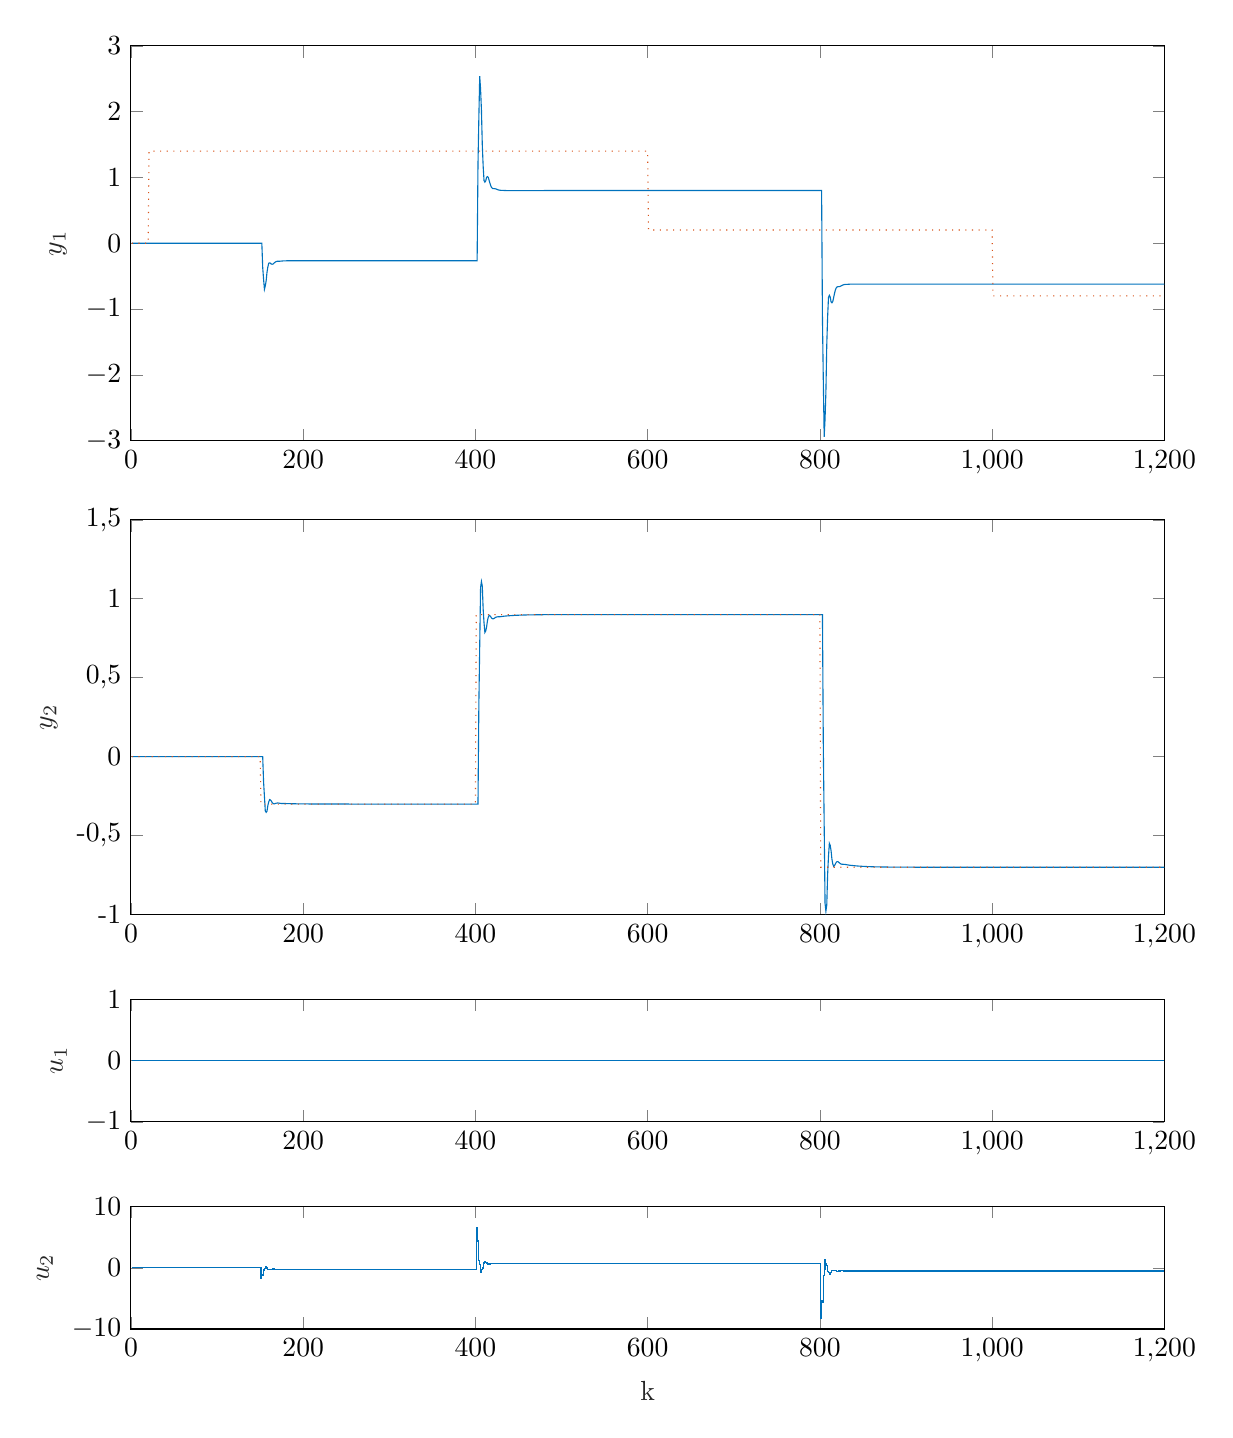
\begin{tikzpicture}

\begin{axis}[%
width=5.167in,
height=0.612in,
at={(0.646in,0.494in)},
scale only axis,
xmin=0,
xmax=1200,
xtick={0,200,400,600,800,1000,1200},
xlabel style={font=\color{white!15!black}},
xlabel={k},
ymin=-10,
ymax=10,
ytick={-10,0,10},
ylabel style={font=\color{white!15!black}},
ylabel={$\text{u}_\text{2}$},
axis background/.style={fill=white}
]
\addplot[const plot, color=mycolor1, forget plot] table[row sep=crcr] {%
1	0\\
2	0\\
3	0\\
4	0\\
5	0\\
6	0\\
7	0\\
8	0\\
9	0\\
10	0\\
11	0\\
12	0\\
13	0\\
14	0\\
15	0\\
16	0\\
17	0\\
18	0\\
19	0\\
20	0\\
21	0\\
22	0\\
23	0\\
24	0\\
25	0\\
26	0\\
27	0\\
28	0\\
29	0\\
30	0\\
31	0\\
32	0\\
33	0\\
34	0\\
35	0\\
36	0\\
37	0\\
38	0\\
39	0\\
40	0\\
41	0\\
42	0\\
43	0\\
44	0\\
45	0\\
46	0\\
47	0\\
48	0\\
49	0\\
50	0\\
51	0\\
52	0\\
53	0\\
54	0\\
55	0\\
56	0\\
57	0\\
58	0\\
59	0\\
60	0\\
61	0\\
62	0\\
63	0\\
64	0\\
65	0\\
66	0\\
67	0\\
68	0\\
69	0\\
70	0\\
71	0\\
72	0\\
73	0\\
74	0\\
75	0\\
76	0\\
77	0\\
78	0\\
79	0\\
80	0\\
81	0\\
82	0\\
83	0\\
84	0\\
85	0\\
86	0\\
87	0\\
88	0\\
89	0\\
90	0\\
91	0\\
92	0\\
93	0\\
94	0\\
95	0\\
96	0\\
97	0\\
98	0\\
99	0\\
100	0\\
101	0\\
102	0\\
103	0\\
104	0\\
105	0\\
106	0\\
107	0\\
108	0\\
109	0\\
110	0\\
111	0\\
112	0\\
113	0\\
114	0\\
115	0\\
116	0\\
117	0\\
118	0\\
119	0\\
120	0\\
121	0\\
122	0\\
123	0\\
124	0\\
125	0\\
126	0\\
127	0\\
128	0\\
129	0\\
130	0\\
131	0\\
132	0\\
133	0\\
134	0\\
135	0\\
136	0\\
137	0\\
138	0\\
139	0\\
140	0\\
141	0\\
142	0\\
143	0\\
144	0\\
145	0\\
146	0\\
147	0\\
148	0\\
149	0\\
150	0\\
151	-1.68475\\
152	-1.12125\\
153	-1.17875\\
154	-0.355736422736457\\
155	-0.182442463673081\\
156	0.133539883128637\\
157	0.00357569302754235\\
158	-0.0470778419975246\\
159	-0.226717837083248\\
160	-0.271530449802226\\
161	-0.315851479324673\\
162	-0.276118937023376\\
163	-0.250237591885371\\
164	-0.210736565716769\\
165	-0.201599296895201\\
166	-0.198009703778164\\
167	-0.209833467499791\\
168	-0.218219467293394\\
169	-0.226517536478594\\
170	-0.227810777596302\\
171	-0.227137127591581\\
172	-0.223866250182907\\
173	-0.221673212107589\\
174	-0.220139154816782\\
175	-0.220209143388749\\
176	-0.22076725083216\\
177	-0.221682144233814\\
178	-0.222245172306459\\
179	-0.222533216465584\\
180	-0.222462818103196\\
181	-0.222294979842552\\
182	-0.222102291338007\\
183	-0.222015674058359\\
184	-0.222010930569533\\
185	-0.222079612777202\\
186	-0.222159858301401\\
187	-0.222230046117523\\
188	-0.222268340149018\\
189	-0.222283805210331\\
190	-0.222284058478431\\
191	-0.222283619481432\\
192	-0.222287632189491\\
193	-0.222299059025489\\
194	-0.222314809004916\\
195	-0.22233212575071\\
196	-0.222347806661917\\
197	-0.222360924295141\\
198	-0.222371383592999\\
199	-0.222380211307956\\
200	-0.222388260708287\\
201	-0.222396243305188\\
202	-0.222404314343296\\
203	-0.222412399588285\\
204	-0.222420236571994\\
205	-0.222427638276309\\
206	-0.222434497918221\\
207	-0.222440838896641\\
208	-0.222446734788458\\
209	-0.222452281811276\\
210	-0.222457546572061\\
211	-0.222462566532152\\
212	-0.222467348526115\\
213	-0.222471888983632\\
214	-0.222476182977483\\
215	-0.22248023403212\\
216	-0.22248405294895\\
217	-0.222487656065605\\
218	-0.222491060276673\\
219	-0.222494280751021\\
220	-0.222497329360644\\
221	-0.2225002153866\\
222	-0.222502946400563\\
223	-0.222505529498202\\
224	-0.222507971835077\\
225	-0.22251028084741\\
226	-0.222512464013633\\
227	-0.222514528598686\\
228	-0.222516481402972\\
229	-0.222518328691022\\
230	-0.222520076212238\\
231	-0.222521729306177\\
232	-0.222523292997957\\
233	-0.222524772072245\\
234	-0.222526171100455\\
235	-0.222527494443945\\
236	-0.222528746242448\\
237	-0.222529930407754\\
238	-0.222531050625303\\
239	-0.222532110366192\\
240	-0.222533112903469\\
241	-0.222534061329411\\
242	-0.222534958569759\\
243	-0.222535807394661\\
244	-0.222536610426585\\
245	-0.222537370146844\\
246	-0.222538088901732\\
247	-0.222538768909039\\
248	-0.222539412264908\\
249	-0.222540020950834\\
250	-0.22254059684041\\
251	-0.222541141705602\\
252	-0.222541657222468\\
253	-0.222542144976373\\
254	-0.222542606466824\\
255	-0.222543043112033\\
256	-0.222543456253267\\
257	-0.222543847159026\\
258	-0.222544217029032\\
259	-0.222544566998006\\
260	-0.222544898139246\\
261	-0.222545211467978\\
262	-0.222545507944519\\
263	-0.222545788477253\\
264	-0.222546053925445\\
265	-0.2225463051019\\
266	-0.222546542775489\\
267	-0.22254676767353\\
268	-0.222546980484052\\
269	-0.222547181857923\\
270	-0.22254737241087\\
271	-0.222547552725381\\
272	-0.222547723352512\\
273	-0.222547884813582\\
274	-0.222548037601789\\
275	-0.222548182183729\\
276	-0.222548319000835\\
277	-0.222548448470741\\
278	-0.22254857098857\\
279	-0.222548686928149\\
280	-0.222548796643163\\
281	-0.22254890046824\\
282	-0.222548998719985\\
283	-0.222549091697952\\
284	-0.222549179685562\\
285	-0.222549262950981\\
286	-0.222549341747936\\
287	-0.222549416316498\\
288	-0.222549486883821\\
289	-0.222549553664832\\
290	-0.222549616862897\\
291	-0.222549676670443\\
292	-0.222549733269545\\
293	-0.222549786832489\\
294	-0.222549837522294\\
295	-0.222549885493215\\
296	-0.222549930891216\\
297	-0.222549973854411\\
298	-0.222550014513494\\
299	-0.222550052992133\\
300	-0.22255008940735\\
301	-0.222550123869882\\
302	-0.222550156484514\\
303	-0.222550187350403\\
304	-0.222550216561378\\
305	-0.222550244206231\\
306	-0.222550270368983\\
307	-0.222550295129144\\
308	-0.222550318561954\\
309	-0.222550340738613\\
310	-0.222550361726499\\
311	-0.222550381589373\\
312	-0.222550400387572\\
313	-0.222550418178194\\
314	-0.222550435015274\\
315	-0.222550450949947\\
316	-0.222550466030601\\
317	-0.222550480303031\\
318	-0.222550493810572\\
319	-0.222550506594235\\
320	-0.22255051869283\\
321	-0.222550530143086\\
322	-0.222550540979759\\
323	-0.222550551235744\\
324	-0.222550560942169\\
325	-0.222550570128494\\
326	-0.222550578822598\\
327	-0.222550587050864\\
328	-0.222550594838261\\
329	-0.22255060220842\\
330	-0.222550609183702\\
331	-0.222550615785272\\
332	-0.222550622033157\\
333	-0.222550627946313\\
334	-0.222550633542678\\
335	-0.222550638839228\\
336	-0.22255064385203\\
337	-0.22255064859629\\
338	-0.222550653086397\\
339	-0.22255065733597\\
340	-0.222550661357899\\
341	-0.222550665164379\\
342	-0.222550668766956\\
343	-0.222550672176554\\
344	-0.222550675403513\\
345	-0.222550678457619\\
346	-0.222550681348132\\
347	-0.222550684083817\\
348	-0.222550686672969\\
349	-0.222550689123438\\
350	-0.222550691442654\\
351	-0.22255069363765\\
352	-0.222550695715078\\
353	-0.222550697681238\\
354	-0.222550699542089\\
355	-0.222550701303274\\
356	-0.222550702970131\\
357	-0.222550704547713\\
358	-0.222550706040803\\
359	-0.222550707453925\\
360	-0.222550708791365\\
361	-0.222550710057175\\
362	-0.222550711255193\\
363	-0.222550712389049\\
364	-0.222550713462181\\
365	-0.222550714477841\\
366	-0.222550715439107\\
367	-0.222550716348892\\
368	-0.222550717209954\\
369	-0.222550718024903\\
370	-0.222550718796209\\
371	-0.222550719526209\\
372	-0.222550720217115\\
373	-0.222550720871021\\
374	-0.222550721489909\\
375	-0.222550722075654\\
376	-0.222550722630031\\
377	-0.22255072315472\\
378	-0.222550723651311\\
379	-0.222550724121309\\
380	-0.222550724566139\\
381	-0.222550724987147\\
382	-0.222550725385611\\
383	-0.222550725762736\\
384	-0.222550726119667\\
385	-0.222550726457483\\
386	-0.22255072677721\\
387	-0.222550727079816\\
388	-0.222550727366219\\
389	-0.222550727637284\\
390	-0.222550727893834\\
391	-0.222550728136646\\
392	-0.222550728366456\\
393	-0.222550728583959\\
394	-0.222550728789816\\
395	-0.222550728984649\\
396	-0.22255072916905\\
397	-0.222550729343577\\
398	-0.222550729508758\\
399	-0.222550729665095\\
400	-0.22255072981306\\
401	6.5164492700469\\
402	4.26244926991436\\
403	4.49244926978891\\
404	1.20039496061601\\
405	0.507219124250139\\
406	-0.75671026306309\\
407	-0.236853502759371\\
408	-0.034239362754372\\
409	0.684320617498353\\
410	0.863571068288927\\
411	1.04085518629795\\
412	0.881925017016312\\
413	0.778399636391943\\
414	0.620395531649057\\
415	0.583846456297976\\
416	0.569488083768488\\
417	0.616783138596938\\
418	0.650327137716405\\
419	0.683519414405196\\
420	0.688692378826809\\
421	0.685997778761337\\
422	0.672914269082552\\
423	0.664142116739549\\
424	0.658005887536828\\
425	0.658285841787316\\
426	0.660518271525581\\
427	0.66417784509871\\
428	0.666429957357599\\
429	0.667582133964105\\
430	0.667300540486165\\
431	0.666629187416719\\
432	0.665858433373112\\
433	0.665511964230453\\
434	0.665492990252366\\
435	0.665767719061482\\
436	0.666088701137872\\
437	0.666369452383045\\
438	0.66652262849074\\
439	0.666584488718691\\
440	0.666585501774718\\
441	0.666583745771225\\
442	0.666599796588794\\
443	0.666645503918906\\
444	0.666708503823474\\
445	0.666777770794217\\
446	0.666840494427273\\
447	0.666892964949027\\
448	0.666934802129912\\
449	0.666970112979764\\
450	0.66700231057164\\
451	0.667034240950309\\
452	0.667066525094278\\
453	0.667098866066227\\
454	0.667130213993483\\
455	0.667159820803572\\
456	0.66718725936443\\
457	0.667212623271688\\
458	0.667236206832878\\
459	0.667258394918395\\
460	0.667279453956084\\
461	0.667299533791292\\
462	0.667318661762265\\
463	0.667336823587717\\
464	0.66735399955875\\
465	0.667370203773163\\
466	0.667385479436573\\
467	0.667399891899485\\
468	0.667413508740252\\
469	0.66742639063432\\
470	0.667438585069673\\
471	0.667450129170522\\
472	0.667461053223563\\
473	0.667471385611454\\
474	0.667481154956437\\
475	0.66749039100338\\
476	0.667499123666016\\
477	0.667507382004089\\
478	0.667515193219211\\
479	0.667522582369493\\
480	0.667529572452548\\
481	0.667536184826587\\
482	0.667542439592084\\
483	0.6675483558877\\
484	0.667553951999087\\
485	0.667559245371668\\
486	0.667564252564377\\
487	0.667568989224363\\
488	0.667573470093392\\
489	0.667577709055844\\
490	0.66758171920391\\
491	0.667585512906692\\
492	0.667589101867145\\
493	0.66759249716587\\
494	0.667595709292726\\
495	0.667598748172967\\
496	0.667601623191769\\
497	0.667604343220287\\
498	0.667606916643089\\
499	0.667609351386157\\
500	0.667611654943856\\
501	0.667613834404054\\
502	0.667615896470977\\
503	0.667617847486088\\
504	0.667619693447413\\
505	0.667621440027791\\
506	0.667623092592293\\
507	0.667624656214919\\
508	0.667626135694551\\
509	0.667627535570081\\
510	0.667628860134692\\
511	0.66763011344929\\
512	0.667631299355142\\
513	0.667632421485784\\
514	0.667633483278272\\
515	0.66763448798383\\
516	0.667635438677937\\
517	0.667636338269869\\
518	0.667637189511733\\
519	0.667637995007003\\
520	0.667638757218584\\
521	0.667639478476437\\
522	0.667640160984778\\
523	0.667640806828889\\
524	0.667641417981556\\
525	0.667641996309163\\
526	0.667642543577444\\
527	0.667643061456936\\
528	0.667643551528125\\
529	0.667644015286322\\
530	0.66764445414626\\
531	0.667644869446459\\
532	0.667645262453337\\
533	0.667645634365105\\
534	0.667645986315458\\
535	0.667646319377046\\
536	0.667646634564783\\
537	0.667646932838955\\
538	0.667647215108167\\
539	0.667647482232139\\
540	0.667647735024333\\
541	0.667647974254454\\
542	0.667648200650805\\
543	0.667648414902524\\
544	0.667648617661693\\
545	0.66764880954533\\
546	0.667648991137284\\
547	0.667649162990019\\
548	0.667649325626304\\
549	0.667649479540815\\
550	0.667649625201644\\
551	0.667649763051734\\
552	0.667649893510226\\
553	0.667650016973746\\
554	0.667650133817615\\
555	0.667650244396997\\
556	0.667650349047978\\
557	0.667650448088597\\
558	0.667650541819813\\
559	0.667650630526427\\
560	0.667650714477949\\
561	0.667650793929421\\
562	0.667650869122194\\
563	0.667650940284663\\
564	0.667651007632965\\
565	0.667651071371635\\
566	0.667651131694235\\
567	0.667651188783937\\
568	0.667651242814084\\
569	0.66765129394872\\
570	0.667651342343088\\
571	0.667651388144099\\
572	0.667651431490784\\
573	0.667651472514715\\
574	0.667651511340406\\
575	0.667651548085697\\
576	0.667651582862102\\
577	0.667651615775157\\
578	0.667651646924739\\
579	0.667651676405366\\
580	0.667651704306489\\
581	0.667651730712761\\
582	0.667651755704296\\
583	0.667651779356913\\
584	0.667651801742368\\
585	0.667651822928563\\
586	0.667651842979768\\
587	0.667651861956802\\
588	0.667651879917227\\
589	0.667651896915517\\
590	0.667651913003227\\
591	0.667651928229147\\
592	0.667651942639452\\
593	0.667651956277842\\
594	0.667651969185676\\
595	0.667651981402095\\
596	0.667651992964144\\
597	0.667652003906881\\
598	0.667652014263485\\
599	0.66765202406536\\
600	0.667652033342222\\
601	0.667652042122198\\
602	0.667652050431909\\
603	0.667652058296546\\
604	0.667652065739952\\
605	0.667652072784689\\
606	0.667652079452114\\
607	0.667652085762441\\
608	0.667652091734796\\
609	0.667652097387286\\
610	0.667652102737042\\
611	0.667652107800282\\
612	0.667652112592352\\
613	0.667652117127777\\
614	0.667652121420304\\
615	0.667652125482942\\
616	0.667652129328004\\
617	0.667652132967145\\
618	0.667652136411394\\
619	0.66765213967119\\
620	0.667652142756411\\
621	0.667652145676409\\
622	0.667652148440031\\
623	0.667652151055653\\
624	0.667652153531202\\
625	0.667652155874181\\
626	0.667652158091688\\
627	0.667652160190445\\
628	0.667652162176811\\
629	0.667652164056804\\
630	0.667652165836121\\
631	0.667652167520156\\
632	0.667652169114009\\
633	0.667652170622513\\
634	0.667652172050235\\
635	0.667652173401503\\
636	0.66765217468041\\
637	0.667652175890832\\
638	0.667652177036438\\
639	0.667652178120698\\
640	0.667652179146897\\
641	0.667652180118144\\
642	0.667652181037383\\
643	0.667652181907398\\
644	0.667652182730826\\
645	0.667652183510162\\
646	0.667652184247766\\
647	0.667652184945872\\
648	0.667652185606597\\
649	0.667652186231941\\
650	0.667652186823799\\
651	0.667652187383965\\
652	0.667652187914136\\
653	0.667652188415919\\
654	0.667652188890832\\
655	0.667652189340316\\
656	0.667652189765732\\
657	0.667652190168368\\
658	0.667652190549446\\
659	0.667652190910117\\
660	0.667652191251476\\
661	0.667652191574556\\
662	0.667652191880337\\
663	0.667652192169745\\
664	0.667652192443655\\
665	0.667652192702899\\
666	0.667652192948261\\
667	0.667652193180485\\
668	0.667652193400274\\
669	0.667652193608295\\
670	0.667652193805178\\
671	0.667652193991519\\
672	0.667652194167883\\
673	0.667652194334805\\
674	0.667652194492788\\
675	0.667652194642312\\
676	0.667652194783829\\
677	0.66765219491777\\
678	0.667652195044538\\
679	0.667652195164518\\
680	0.667652195278074\\
681	0.667652195385549\\
682	0.66765219548727\\
683	0.667652195583545\\
684	0.667652195674664\\
685	0.667652195760905\\
686	0.667652195842528\\
687	0.66765219591978\\
688	0.667652195992895\\
689	0.667652196062095\\
690	0.667652196127589\\
691	0.667652196189578\\
692	0.667652196248247\\
693	0.667652196303776\\
694	0.667652196356332\\
695	0.667652196406074\\
696	0.667652196453152\\
697	0.66765219649771\\
698	0.667652196539881\\
699	0.667652196579795\\
700	0.66765219661757\\
701	0.667652196653323\\
702	0.667652196687162\\
703	0.66765219671919\\
704	0.667652196749502\\
705	0.667652196778191\\
706	0.667652196805344\\
707	0.667652196831043\\
708	0.667652196855366\\
709	0.667652196878387\\
710	0.667652196900175\\
711	0.667652196920797\\
712	0.667652196940314\\
713	0.667652196958787\\
714	0.667652196976271\\
715	0.667652196992818\\
716	0.66765219700848\\
717	0.667652197023303\\
718	0.667652197037332\\
719	0.66765219705061\\
720	0.667652197063176\\
721	0.667652197075071\\
722	0.667652197086327\\
723	0.667652197096982\\
724	0.667652197107066\\
725	0.667652197116611\\
726	0.667652197125644\\
727	0.667652197134193\\
728	0.667652197142284\\
729	0.667652197149943\\
730	0.667652197157192\\
731	0.667652197164053\\
732	0.667652197170546\\
733	0.667652197176693\\
734	0.667652197182509\\
735	0.667652197188015\\
736	0.667652197193225\\
737	0.667652197198156\\
738	0.667652197202822\\
739	0.667652197207238\\
740	0.667652197211417\\
741	0.667652197215374\\
742	0.667652197219118\\
743	0.667652197222664\\
744	0.667652197226019\\
745	0.667652197229194\\
746	0.667652197232199\\
747	0.667652197235045\\
748	0.667652197237737\\
749	0.667652197240285\\
750	0.667652197242696\\
751	0.667652197244978\\
752	0.667652197247139\\
753	0.667652197249184\\
754	0.66765219725112\\
755	0.667652197252951\\
756	0.667652197254683\\
757	0.667652197256322\\
758	0.667652197257874\\
759	0.667652197259344\\
760	0.667652197260735\\
761	0.66765219726205\\
762	0.667652197263296\\
763	0.667652197264476\\
764	0.667652197265593\\
765	0.667652197266651\\
766	0.667652197267651\\
767	0.667652197268597\\
768	0.667652197269492\\
769	0.667652197270338\\
770	0.66765219727114\\
771	0.667652197271898\\
772	0.667652197272616\\
773	0.667652197273296\\
774	0.667652197273939\\
775	0.667652197274548\\
776	0.667652197275125\\
777	0.66765219727567\\
778	0.667652197276186\\
779	0.667652197276674\\
780	0.667652197277137\\
781	0.667652197277574\\
782	0.667652197277988\\
783	0.66765219727838\\
784	0.667652197278752\\
785	0.667652197279103\\
786	0.667652197279436\\
787	0.667652197279751\\
788	0.66765219728005\\
789	0.667652197280333\\
790	0.667652197280601\\
791	0.667652197280854\\
792	0.667652197281093\\
793	0.667652197281319\\
794	0.667652197281532\\
795	0.667652197281735\\
796	0.667652197281927\\
797	0.667652197282108\\
798	0.66765219728228\\
799	0.667652197282443\\
800	0.667652197282598\\
801	-8.31768113605059\\
802	-5.31234780271711\\
803	-5.61901446938365\\
804	-1.22960872397797\\
805	-0.305374275639846\\
806	1.37986490730276\\
807	0.686722560097032\\
808	0.416570373296774\\
809	-0.541509600493655\\
810	-0.78051020166145\\
811	-1.01688902578108\\
812	-0.804982133507415\\
813	-0.666948292771317\\
814	-0.456276153205367\\
815	-0.407544052823609\\
816	-0.388399556199347\\
817	-0.451459629381298\\
818	-0.496184961613795\\
819	-0.540441330601472\\
820	-0.547338616562534\\
821	-0.543745816537305\\
822	-0.526301137024334\\
823	-0.514604933955923\\
824	-0.506423295071581\\
825	-0.506796567455368\\
826	-0.509773140486857\\
827	-0.514652571962306\\
828	-0.517655388349714\\
829	-0.519191623865018\\
830	-0.518816165932253\\
831	-0.517921028542122\\
832	-0.516893356517859\\
833	-0.516431397693049\\
834	-0.516406099085949\\
835	-0.516772404193495\\
836	-0.517200380322536\\
837	-0.517574715341831\\
838	-0.517778950176446\\
839	-0.517861430503431\\
840	-0.517862781266615\\
841	-0.517860439949273\\
842	-0.517881841058906\\
843	-0.517942784184218\\
844	-0.51802678407448\\
845	-0.518119140052038\\
846	-0.518202771578459\\
847	-0.518272732288972\\
848	-0.518328515210864\\
849	-0.518375596357294\\
850	-0.518418526492379\\
851	-0.518461100342513\\
852	-0.518504145879077\\
853	-0.518547267185678\\
854	-0.518589064432116\\
855	-0.518628540188456\\
856	-0.518665124945308\\
857	-0.518698943496876\\
858	-0.518730388253229\\
859	-0.518759972374919\\
860	-0.518788051099096\\
861	-0.518814824219578\\
862	-0.518840328187378\\
863	-0.518864543960801\\
864	-0.518887445261334\\
865	-0.518909050886062\\
866	-0.51892941844249\\
867	-0.518948635064642\\
868	-0.518966790857007\\
869	-0.518983966720187\\
870	-0.51900022597151\\
871	-0.519015618109936\\
872	-0.519030183517737\\
873	-0.519043960038472\\
874	-0.519056985835142\\
875	-0.519069300567579\\
876	-0.519080944120771\\
877	-0.519091955241047\\
878	-0.519102370197238\\
879	-0.519112222400164\\
880	-0.519121542513318\\
881	-0.519130359014321\\
882	-0.519138698703815\\
883	-0.519146587100017\\
884	-0.519154048583804\\
885	-0.519161106415747\\
886	-0.519167782674429\\
887	-0.519174098222722\\
888	-0.519180072716315\\
889	-0.51918572466772\\
890	-0.5191910715332\\
891	-0.519196129804891\\
892	-0.519200915086741\\
893	-0.519205442152888\\
894	-0.519209724989814\\
895	-0.519213776831193\\
896	-0.519217610190596\\
897	-0.519221236896234\\
898	-0.519224668127534\\
899	-0.519227914452473\\
900	-0.519230985863542\\
901	-0.519233891811233\\
902	-0.519236641234517\\
903	-0.519239242588678\\
904	-0.519241703871089\\
905	-0.519244032645539\\
906	-0.519246236065453\\
907	-0.519248320896169\\
908	-0.519250293536196\\
909	-0.519252160037392\\
910	-0.519253926124002\\
911	-0.519255597210571\\
912	-0.519257178418788\\
913	-0.519258674593369\\
914	-0.519260090317058\\
915	-0.519261429924822\\
916	-0.519262697517298\\
917	-0.519263896973524\\
918	-0.519265031962975\\
919	-0.519266105956949\\
920	-0.519267122239323\\
921	-0.519268083916713\\
922	-0.519268993928074\\
923	-0.519269855053782\\
924	-0.519270669924222\\
925	-0.5192714410279\\
926	-0.519272170719134\\
927	-0.519272861225303\\
928	-0.519273514653726\\
929	-0.519274132998149\\
930	-0.519274718144887\\
931	-0.519275271878632\\
932	-0.51927579588794\\
933	-0.519276291770429\\
934	-0.51927676103769\\
935	-0.519277205119925\\
936	-0.519277625370352\\
937	-0.519278023069352\\
938	-0.5192783994284\\
939	-0.519278755593788\\
940	-0.519279092650134\\
941	-0.519279411623709\\
942	-0.519279713485591\\
943	-0.519279999154625\\
944	-0.519280269500255\\
945	-0.519280525345171\\
946	-0.51928076746784\\
947	-0.519280996604881\\
948	-0.519281213453321\\
949	-0.519281418672726\\
950	-0.519281612887218\\
951	-0.519281796687386\\
952	-0.519281970632089\\
953	-0.519282135250159\\
954	-0.519282291042027\\
955	-0.519282438481242\\
956	-0.51928257801592\\
957	-0.519282710070112\\
958	-0.519282835045099\\
959	-0.519282953320615\\
960	-0.519283065256009\\
961	-0.519283171191334\\
962	-0.519283271448392\\
963	-0.519283366331709\\
964	-0.519283456129469\\
965	-0.519283541114385\\
966	-0.51928362154454\\
967	-0.519283697664163\\
968	-0.519283769704379\\
969	-0.519283837883912\\
970	-0.519283902409752\\
971	-0.519283963477781\\
972	-0.519284021273373\\
973	-0.519284075971961\\
974	-0.519284127739565\\
975	-0.519284176733299\\
976	-0.519284223101853\\
977	-0.519284266985939\\
978	-0.519284308518726\\
979	-0.519284347826238\\
980	-0.519284385027744\\
981	-0.519284420236114\\
982	-0.519284453558169\\
983	-0.519284485095001\\
984	-0.519284514942281\\
985	-0.51928454319055\\
986	-0.519284569925498\\
987	-0.519284595228219\\
988	-0.519284619175459\\
989	-0.519284641839851\\
990	-0.519284663290134\\
991	-0.519284683591364\\
992	-0.519284702805107\\
993	-0.519284720989631\\
994	-0.519284738200081\\
995	-0.519284754488646\\
996	-0.519284769904716\\
997	-0.519284784495037\\
998	-0.519284798303848\\
999	-0.519284811373017\\
1000	-0.519284823742171\\
1001	-0.519284835448811\\
1002	-0.519284846528428\\
1003	-0.519284857014612\\
1004	-0.519284866939155\\
1005	-0.51928487633214\\
1006	-0.519284885222043\\
1007	-0.519284893635814\\
1008	-0.519284901598957\\
1009	-0.519284909135611\\
1010	-0.519284916268622\\
1011	-0.519284923019609\\
1012	-0.519284929409038\\
1013	-0.519284935456272\\
1014	-0.519284941179642\\
1015	-0.519284946596494\\
1016	-0.519284951723246\\
1017	-0.519284956575435\\
1018	-0.519284961167769\\
1019	-0.519284965514166\\
1020	-0.519284969627797\\
1021	-0.519284973521129\\
1022	-0.519284977205961\\
1023	-0.519284980693459\\
1024	-0.519284983994194\\
1025	-0.519284987118167\\
1026	-0.519284990074844\\
1027	-0.519284992873187\\
1028	-0.519284995521673\\
1029	-0.51928499802833\\
1030	-0.519285000400754\\
1031	-0.519285002646133\\
1032	-0.519285004771272\\
1033	-0.519285006782609\\
1034	-0.519285008686238\\
1035	-0.519285010487928\\
1036	-0.519285012193139\\
1037	-0.519285013807036\\
1038	-0.51928501533451\\
1039	-0.519285016780189\\
1040	-0.519285018148455\\
1041	-0.519285019443453\\
1042	-0.519285020669105\\
1043	-0.519285021829127\\
1044	-0.519285022927031\\
1045	-0.519285023966145\\
1046	-0.519285024949617\\
1047	-0.519285025880425\\
1048	-0.519285026761391\\
1049	-0.519285027595183\\
1050	-0.519285028384328\\
1051	-0.519285029131217\\
1052	-0.519285029838112\\
1053	-0.519285030507156\\
1054	-0.519285031140374\\
1055	-0.519285031739686\\
1056	-0.519285032306906\\
1057	-0.519285032843753\\
1058	-0.519285033351854\\
1059	-0.519285033832749\\
1060	-0.519285034287894\\
1061	-0.519285034718669\\
1062	-0.519285035126378\\
1063	-0.519285035512255\\
1064	-0.51928503587747\\
1065	-0.519285036223129\\
1066	-0.519285036550279\\
1067	-0.519285036859912\\
1068	-0.519285037152966\\
1069	-0.519285037430327\\
1070	-0.519285037692839\\
1071	-0.519285037941293\\
1072	-0.519285038176445\\
1073	-0.519285038399005\\
1074	-0.519285038609649\\
1075	-0.519285038809013\\
1076	-0.519285038997703\\
1077	-0.519285039176289\\
1078	-0.519285039345314\\
1079	-0.519285039505287\\
1080	-0.519285039656695\\
1081	-0.519285039799994\\
1082	-0.51928503993562\\
1083	-0.519285040063985\\
1084	-0.519285040185477\\
1085	-0.519285040300465\\
1086	-0.519285040409295\\
1087	-0.519285040512299\\
1088	-0.519285040609788\\
1089	-0.519285040702056\\
1090	-0.519285040789384\\
1091	-0.519285040872035\\
1092	-0.519285040950261\\
1093	-0.519285041024299\\
1094	-0.519285041094372\\
1095	-0.519285041160693\\
1096	-0.519285041223463\\
1097	-0.519285041282872\\
1098	-0.5192850413391\\
1099	-0.519285041392318\\
1100	-0.519285041442687\\
1101	-0.519285041490357\\
1102	-0.519285041535476\\
1103	-0.519285041578179\\
1104	-0.519285041618596\\
1105	-0.51928504165685\\
1106	-0.519285041693055\\
1107	-0.519285041727321\\
1108	-0.519285041759753\\
1109	-0.519285041790448\\
1110	-0.519285041819498\\
1111	-0.519285041846994\\
1112	-0.519285041873019\\
1113	-0.51928504189765\\
1114	-0.519285041920962\\
1115	-0.519285041943025\\
1116	-0.519285041963906\\
1117	-0.519285041983671\\
1118	-0.519285042002377\\
1119	-0.519285042020082\\
1120	-0.519285042036838\\
1121	-0.519285042052698\\
1122	-0.519285042067706\\
1123	-0.519285042081911\\
1124	-0.519285042095356\\
1125	-0.519285042108082\\
1126	-0.519285042120127\\
1127	-0.519285042131526\\
1128	-0.519285042142315\\
1129	-0.519285042152526\\
1130	-0.519285042162191\\
1131	-0.519285042171339\\
1132	-0.519285042179996\\
1133	-0.51928504218819\\
1134	-0.519285042195945\\
1135	-0.519285042203285\\
1136	-0.519285042210232\\
1137	-0.519285042216806\\
1138	-0.51928504222303\\
1139	-0.519285042228919\\
1140	-0.519285042234493\\
1141	-0.51928504223977\\
1142	-0.519285042244764\\
1143	-0.51928504224949\\
1144	-0.519285042253963\\
1145	-0.519285042258195\\
1146	-0.519285042262201\\
1147	-0.519285042265992\\
1148	-0.519285042269582\\
1149	-0.51928504227298\\
1150	-0.519285042276197\\
1151	-0.519285042279241\\
1152	-0.519285042282121\\
1153	-0.519285042284846\\
1154	-0.519285042287425\\
1155	-0.519285042289866\\
1156	-0.519285042292178\\
1157	-0.519285042294366\\
1158	-0.519285042296437\\
1159	-0.519285042298397\\
1160	-0.519285042300251\\
1161	-0.519285042302006\\
1162	-0.519285042303668\\
1163	-0.51928504230524\\
1164	-0.519285042306728\\
1165	-0.519285042308136\\
1166	-0.519285042309468\\
1167	-0.51928504231073\\
1168	-0.519285042311923\\
1169	-0.519285042313053\\
1170	-0.519285042314121\\
1171	-0.519285042315133\\
1172	-0.519285042316091\\
1173	-0.519285042316998\\
1174	-0.519285042317857\\
1175	-0.519285042318669\\
1176	-0.519285042319439\\
1177	-0.519285042320166\\
1178	-0.519285042320854\\
1179	-0.519285042321505\\
1180	-0.519285042322122\\
1181	-0.519285042322705\\
1182	-0.519285042323257\\
1183	-0.51928504232378\\
1184	-0.519285042324275\\
1185	-0.519285042324744\\
1186	-0.519285042325188\\
1187	-0.519285042325608\\
1188	-0.519285042326007\\
1189	-0.519285042326384\\
1190	-0.519285042326741\\
1191	-0.519285042327078\\
1192	-0.519285042327396\\
1193	-0.519285042327697\\
1194	-0.519285042327981\\
1195	-0.519285042328251\\
1196	-0.519285042328506\\
1197	-0.519285042328749\\
1198	-0.519285042328977\\
1199	-0.519285042329194\\
1200	-0.519285042329399\\
};
\end{axis}

\begin{axis}[%
width=5.167in,
height=0.612in,
at={(0.646in,1.53in)},
scale only axis,
xmin=0,
xmax=1200,
xtick={0,200,400,600,800,1000,1200},
ymin=-1,
ymax=1,
ytick={-1,0,1},
ylabel style={font=\color{white!15!black}},
ylabel={$\text{u}_\text{1}$},
axis background/.style={fill=white}
]
\addplot[const plot, color=mycolor1, forget plot] table[row sep=crcr] {%
1	0\\
2	0\\
3	0\\
4	0\\
5	0\\
6	0\\
7	0\\
8	0\\
9	0\\
10	0\\
11	0\\
12	0\\
13	0\\
14	0\\
15	0\\
16	0\\
17	0\\
18	0\\
19	0\\
20	0\\
21	0\\
22	0\\
23	0\\
24	0\\
25	0\\
26	0\\
27	0\\
28	0\\
29	0\\
30	0\\
31	0\\
32	0\\
33	0\\
34	0\\
35	0\\
36	0\\
37	0\\
38	0\\
39	0\\
40	0\\
41	0\\
42	0\\
43	0\\
44	0\\
45	0\\
46	0\\
47	0\\
48	0\\
49	0\\
50	0\\
51	0\\
52	0\\
53	0\\
54	0\\
55	0\\
56	0\\
57	0\\
58	0\\
59	0\\
60	0\\
61	0\\
62	0\\
63	0\\
64	0\\
65	0\\
66	0\\
67	0\\
68	0\\
69	0\\
70	0\\
71	0\\
72	0\\
73	0\\
74	0\\
75	0\\
76	0\\
77	0\\
78	0\\
79	0\\
80	0\\
81	0\\
82	0\\
83	0\\
84	0\\
85	0\\
86	0\\
87	0\\
88	0\\
89	0\\
90	0\\
91	0\\
92	0\\
93	0\\
94	0\\
95	0\\
96	0\\
97	0\\
98	0\\
99	0\\
100	0\\
101	0\\
102	0\\
103	0\\
104	0\\
105	0\\
106	0\\
107	0\\
108	0\\
109	0\\
110	0\\
111	0\\
112	0\\
113	0\\
114	0\\
115	0\\
116	0\\
117	0\\
118	0\\
119	0\\
120	0\\
121	0\\
122	0\\
123	0\\
124	0\\
125	0\\
126	0\\
127	0\\
128	0\\
129	0\\
130	0\\
131	0\\
132	0\\
133	0\\
134	0\\
135	0\\
136	0\\
137	0\\
138	0\\
139	0\\
140	0\\
141	0\\
142	0\\
143	0\\
144	0\\
145	0\\
146	0\\
147	0\\
148	0\\
149	0\\
150	0\\
151	0\\
152	0\\
153	0\\
154	0\\
155	0\\
156	0\\
157	0\\
158	0\\
159	0\\
160	0\\
161	0\\
162	0\\
163	0\\
164	0\\
165	0\\
166	0\\
167	0\\
168	0\\
169	0\\
170	0\\
171	0\\
172	0\\
173	0\\
174	0\\
175	0\\
176	0\\
177	0\\
178	0\\
179	0\\
180	0\\
181	0\\
182	0\\
183	0\\
184	0\\
185	0\\
186	0\\
187	0\\
188	0\\
189	0\\
190	0\\
191	0\\
192	0\\
193	0\\
194	0\\
195	0\\
196	0\\
197	0\\
198	0\\
199	0\\
200	0\\
201	0\\
202	0\\
203	0\\
204	0\\
205	0\\
206	0\\
207	0\\
208	0\\
209	0\\
210	0\\
211	0\\
212	0\\
213	0\\
214	0\\
215	0\\
216	0\\
217	0\\
218	0\\
219	0\\
220	0\\
221	0\\
222	0\\
223	0\\
224	0\\
225	0\\
226	0\\
227	0\\
228	0\\
229	0\\
230	0\\
231	0\\
232	0\\
233	0\\
234	0\\
235	0\\
236	0\\
237	0\\
238	0\\
239	0\\
240	0\\
241	0\\
242	0\\
243	0\\
244	0\\
245	0\\
246	0\\
247	0\\
248	0\\
249	0\\
250	0\\
251	0\\
252	0\\
253	0\\
254	0\\
255	0\\
256	0\\
257	0\\
258	0\\
259	0\\
260	0\\
261	0\\
262	0\\
263	0\\
264	0\\
265	0\\
266	0\\
267	0\\
268	0\\
269	0\\
270	0\\
271	0\\
272	0\\
273	0\\
274	0\\
275	0\\
276	0\\
277	0\\
278	0\\
279	0\\
280	0\\
281	0\\
282	0\\
283	0\\
284	0\\
285	0\\
286	0\\
287	0\\
288	0\\
289	0\\
290	0\\
291	0\\
292	0\\
293	0\\
294	0\\
295	0\\
296	0\\
297	0\\
298	0\\
299	0\\
300	0\\
301	0\\
302	0\\
303	0\\
304	0\\
305	0\\
306	0\\
307	0\\
308	0\\
309	0\\
310	0\\
311	0\\
312	0\\
313	0\\
314	0\\
315	0\\
316	0\\
317	0\\
318	0\\
319	0\\
320	0\\
321	0\\
322	0\\
323	0\\
324	0\\
325	0\\
326	0\\
327	0\\
328	0\\
329	0\\
330	0\\
331	0\\
332	0\\
333	0\\
334	0\\
335	0\\
336	0\\
337	0\\
338	0\\
339	0\\
340	0\\
341	0\\
342	0\\
343	0\\
344	0\\
345	0\\
346	0\\
347	0\\
348	0\\
349	0\\
350	0\\
351	0\\
352	0\\
353	0\\
354	0\\
355	0\\
356	0\\
357	0\\
358	0\\
359	0\\
360	0\\
361	0\\
362	0\\
363	0\\
364	0\\
365	0\\
366	0\\
367	0\\
368	0\\
369	0\\
370	0\\
371	0\\
372	0\\
373	0\\
374	0\\
375	0\\
376	0\\
377	0\\
378	0\\
379	0\\
380	0\\
381	0\\
382	0\\
383	0\\
384	0\\
385	0\\
386	0\\
387	0\\
388	0\\
389	0\\
390	0\\
391	0\\
392	0\\
393	0\\
394	0\\
395	0\\
396	0\\
397	0\\
398	0\\
399	0\\
400	0\\
401	0\\
402	0\\
403	0\\
404	0\\
405	0\\
406	0\\
407	0\\
408	0\\
409	0\\
410	0\\
411	0\\
412	0\\
413	0\\
414	0\\
415	0\\
416	0\\
417	0\\
418	0\\
419	0\\
420	0\\
421	0\\
422	0\\
423	0\\
424	0\\
425	0\\
426	0\\
427	0\\
428	0\\
429	0\\
430	0\\
431	0\\
432	0\\
433	0\\
434	0\\
435	0\\
436	0\\
437	0\\
438	0\\
439	0\\
440	0\\
441	0\\
442	0\\
443	0\\
444	0\\
445	0\\
446	0\\
447	0\\
448	0\\
449	0\\
450	0\\
451	0\\
452	0\\
453	0\\
454	0\\
455	0\\
456	0\\
457	0\\
458	0\\
459	0\\
460	0\\
461	0\\
462	0\\
463	0\\
464	0\\
465	0\\
466	0\\
467	0\\
468	0\\
469	0\\
470	0\\
471	0\\
472	0\\
473	0\\
474	0\\
475	0\\
476	0\\
477	0\\
478	0\\
479	0\\
480	0\\
481	0\\
482	0\\
483	0\\
484	0\\
485	0\\
486	0\\
487	0\\
488	0\\
489	0\\
490	0\\
491	0\\
492	0\\
493	0\\
494	0\\
495	0\\
496	0\\
497	0\\
498	0\\
499	0\\
500	0\\
501	0\\
502	0\\
503	0\\
504	0\\
505	0\\
506	0\\
507	0\\
508	0\\
509	0\\
510	0\\
511	0\\
512	0\\
513	0\\
514	0\\
515	0\\
516	0\\
517	0\\
518	0\\
519	0\\
520	0\\
521	0\\
522	0\\
523	0\\
524	0\\
525	0\\
526	0\\
527	0\\
528	0\\
529	0\\
530	0\\
531	0\\
532	0\\
533	0\\
534	0\\
535	0\\
536	0\\
537	0\\
538	0\\
539	0\\
540	0\\
541	0\\
542	0\\
543	0\\
544	0\\
545	0\\
546	0\\
547	0\\
548	0\\
549	0\\
550	0\\
551	0\\
552	0\\
553	0\\
554	0\\
555	0\\
556	0\\
557	0\\
558	0\\
559	0\\
560	0\\
561	0\\
562	0\\
563	0\\
564	0\\
565	0\\
566	0\\
567	0\\
568	0\\
569	0\\
570	0\\
571	0\\
572	0\\
573	0\\
574	0\\
575	0\\
576	0\\
577	0\\
578	0\\
579	0\\
580	0\\
581	0\\
582	0\\
583	0\\
584	0\\
585	0\\
586	0\\
587	0\\
588	0\\
589	0\\
590	0\\
591	0\\
592	0\\
593	0\\
594	0\\
595	0\\
596	0\\
597	0\\
598	0\\
599	0\\
600	0\\
601	0\\
602	0\\
603	0\\
604	0\\
605	0\\
606	0\\
607	0\\
608	0\\
609	0\\
610	0\\
611	0\\
612	0\\
613	0\\
614	0\\
615	0\\
616	0\\
617	0\\
618	0\\
619	0\\
620	0\\
621	0\\
622	0\\
623	0\\
624	0\\
625	0\\
626	0\\
627	0\\
628	0\\
629	0\\
630	0\\
631	0\\
632	0\\
633	0\\
634	0\\
635	0\\
636	0\\
637	0\\
638	0\\
639	0\\
640	0\\
641	0\\
642	0\\
643	0\\
644	0\\
645	0\\
646	0\\
647	0\\
648	0\\
649	0\\
650	0\\
651	0\\
652	0\\
653	0\\
654	0\\
655	0\\
656	0\\
657	0\\
658	0\\
659	0\\
660	0\\
661	0\\
662	0\\
663	0\\
664	0\\
665	0\\
666	0\\
667	0\\
668	0\\
669	0\\
670	0\\
671	0\\
672	0\\
673	0\\
674	0\\
675	0\\
676	0\\
677	0\\
678	0\\
679	0\\
680	0\\
681	0\\
682	0\\
683	0\\
684	0\\
685	0\\
686	0\\
687	0\\
688	0\\
689	0\\
690	0\\
691	0\\
692	0\\
693	0\\
694	0\\
695	0\\
696	0\\
697	0\\
698	0\\
699	0\\
700	0\\
701	0\\
702	0\\
703	0\\
704	0\\
705	0\\
706	0\\
707	0\\
708	0\\
709	0\\
710	0\\
711	0\\
712	0\\
713	0\\
714	0\\
715	0\\
716	0\\
717	0\\
718	0\\
719	0\\
720	0\\
721	0\\
722	0\\
723	0\\
724	0\\
725	0\\
726	0\\
727	0\\
728	0\\
729	0\\
730	0\\
731	0\\
732	0\\
733	0\\
734	0\\
735	0\\
736	0\\
737	0\\
738	0\\
739	0\\
740	0\\
741	0\\
742	0\\
743	0\\
744	0\\
745	0\\
746	0\\
747	0\\
748	0\\
749	0\\
750	0\\
751	0\\
752	0\\
753	0\\
754	0\\
755	0\\
756	0\\
757	0\\
758	0\\
759	0\\
760	0\\
761	0\\
762	0\\
763	0\\
764	0\\
765	0\\
766	0\\
767	0\\
768	0\\
769	0\\
770	0\\
771	0\\
772	0\\
773	0\\
774	0\\
775	0\\
776	0\\
777	0\\
778	0\\
779	0\\
780	0\\
781	0\\
782	0\\
783	0\\
784	0\\
785	0\\
786	0\\
787	0\\
788	0\\
789	0\\
790	0\\
791	0\\
792	0\\
793	0\\
794	0\\
795	0\\
796	0\\
797	0\\
798	0\\
799	0\\
800	0\\
801	0\\
802	0\\
803	0\\
804	0\\
805	0\\
806	0\\
807	0\\
808	0\\
809	0\\
810	0\\
811	0\\
812	0\\
813	0\\
814	0\\
815	0\\
816	0\\
817	0\\
818	0\\
819	0\\
820	0\\
821	0\\
822	0\\
823	0\\
824	0\\
825	0\\
826	0\\
827	0\\
828	0\\
829	0\\
830	0\\
831	0\\
832	0\\
833	0\\
834	0\\
835	0\\
836	0\\
837	0\\
838	0\\
839	0\\
840	0\\
841	0\\
842	0\\
843	0\\
844	0\\
845	0\\
846	0\\
847	0\\
848	0\\
849	0\\
850	0\\
851	0\\
852	0\\
853	0\\
854	0\\
855	0\\
856	0\\
857	0\\
858	0\\
859	0\\
860	0\\
861	0\\
862	0\\
863	0\\
864	0\\
865	0\\
866	0\\
867	0\\
868	0\\
869	0\\
870	0\\
871	0\\
872	0\\
873	0\\
874	0\\
875	0\\
876	0\\
877	0\\
878	0\\
879	0\\
880	0\\
881	0\\
882	0\\
883	0\\
884	0\\
885	0\\
886	0\\
887	0\\
888	0\\
889	0\\
890	0\\
891	0\\
892	0\\
893	0\\
894	0\\
895	0\\
896	0\\
897	0\\
898	0\\
899	0\\
900	0\\
901	0\\
902	0\\
903	0\\
904	0\\
905	0\\
906	0\\
907	0\\
908	0\\
909	0\\
910	0\\
911	0\\
912	0\\
913	0\\
914	0\\
915	0\\
916	0\\
917	0\\
918	0\\
919	0\\
920	0\\
921	0\\
922	0\\
923	0\\
924	0\\
925	0\\
926	0\\
927	0\\
928	0\\
929	0\\
930	0\\
931	0\\
932	0\\
933	0\\
934	0\\
935	0\\
936	0\\
937	0\\
938	0\\
939	0\\
940	0\\
941	0\\
942	0\\
943	0\\
944	0\\
945	0\\
946	0\\
947	0\\
948	0\\
949	0\\
950	0\\
951	0\\
952	0\\
953	0\\
954	0\\
955	0\\
956	0\\
957	0\\
958	0\\
959	0\\
960	0\\
961	0\\
962	0\\
963	0\\
964	0\\
965	0\\
966	0\\
967	0\\
968	0\\
969	0\\
970	0\\
971	0\\
972	0\\
973	0\\
974	0\\
975	0\\
976	0\\
977	0\\
978	0\\
979	0\\
980	0\\
981	0\\
982	0\\
983	0\\
984	0\\
985	0\\
986	0\\
987	0\\
988	0\\
989	0\\
990	0\\
991	0\\
992	0\\
993	0\\
994	0\\
995	0\\
996	0\\
997	0\\
998	0\\
999	0\\
1000	0\\
1001	0\\
1002	0\\
1003	0\\
1004	0\\
1005	0\\
1006	0\\
1007	0\\
1008	0\\
1009	0\\
1010	0\\
1011	0\\
1012	0\\
1013	0\\
1014	0\\
1015	0\\
1016	0\\
1017	0\\
1018	0\\
1019	0\\
1020	0\\
1021	0\\
1022	0\\
1023	0\\
1024	0\\
1025	0\\
1026	0\\
1027	0\\
1028	0\\
1029	0\\
1030	0\\
1031	0\\
1032	0\\
1033	0\\
1034	0\\
1035	0\\
1036	0\\
1037	0\\
1038	0\\
1039	0\\
1040	0\\
1041	0\\
1042	0\\
1043	0\\
1044	0\\
1045	0\\
1046	0\\
1047	0\\
1048	0\\
1049	0\\
1050	0\\
1051	0\\
1052	0\\
1053	0\\
1054	0\\
1055	0\\
1056	0\\
1057	0\\
1058	0\\
1059	0\\
1060	0\\
1061	0\\
1062	0\\
1063	0\\
1064	0\\
1065	0\\
1066	0\\
1067	0\\
1068	0\\
1069	0\\
1070	0\\
1071	0\\
1072	0\\
1073	0\\
1074	0\\
1075	0\\
1076	0\\
1077	0\\
1078	0\\
1079	0\\
1080	0\\
1081	0\\
1082	0\\
1083	0\\
1084	0\\
1085	0\\
1086	0\\
1087	0\\
1088	0\\
1089	0\\
1090	0\\
1091	0\\
1092	0\\
1093	0\\
1094	0\\
1095	0\\
1096	0\\
1097	0\\
1098	0\\
1099	0\\
1100	0\\
1101	0\\
1102	0\\
1103	0\\
1104	0\\
1105	0\\
1106	0\\
1107	0\\
1108	0\\
1109	0\\
1110	0\\
1111	0\\
1112	0\\
1113	0\\
1114	0\\
1115	0\\
1116	0\\
1117	0\\
1118	0\\
1119	0\\
1120	0\\
1121	0\\
1122	0\\
1123	0\\
1124	0\\
1125	0\\
1126	0\\
1127	0\\
1128	0\\
1129	0\\
1130	0\\
1131	0\\
1132	0\\
1133	0\\
1134	0\\
1135	0\\
1136	0\\
1137	0\\
1138	0\\
1139	0\\
1140	0\\
1141	0\\
1142	0\\
1143	0\\
1144	0\\
1145	0\\
1146	0\\
1147	0\\
1148	0\\
1149	0\\
1150	0\\
1151	0\\
1152	0\\
1153	0\\
1154	0\\
1155	0\\
1156	0\\
1157	0\\
1158	0\\
1159	0\\
1160	0\\
1161	0\\
1162	0\\
1163	0\\
1164	0\\
1165	0\\
1166	0\\
1167	0\\
1168	0\\
1169	0\\
1170	0\\
1171	0\\
1172	0\\
1173	0\\
1174	0\\
1175	0\\
1176	0\\
1177	0\\
1178	0\\
1179	0\\
1180	0\\
1181	0\\
1182	0\\
1183	0\\
1184	0\\
1185	0\\
1186	0\\
1187	0\\
1188	0\\
1189	0\\
1190	0\\
1191	0\\
1192	0\\
1193	0\\
1194	0\\
1195	0\\
1196	0\\
1197	0\\
1198	0\\
1199	0\\
1200	0\\
};
\end{axis}

\begin{axis}[%
width=5.167in,
height=1.974in,
at={(0.646in,2.566in)},
scale only axis,
xmin=0,
xmax=1200,
xtick={0,200,400,600,800,1000,1200},
ymin=-1,
ymax=1.5,
ytick={-1,-0.5,0,0.5,1,1.5},
yticklabels={{-1},{-0,5},{0},{0,5},{1},{1,5}},
ylabel style={font=\color{white!15!black}},
ylabel={$\text{y}_\text{2}$},
axis background/.style={fill=white}
]
\addplot [color=mycolor1, forget plot]
  table[row sep=crcr]{%
1	0\\
2	0\\
3	0\\
4	0\\
5	0\\
6	0\\
7	0\\
8	0\\
9	0\\
10	0\\
11	0\\
12	0\\
13	0\\
14	0\\
15	0\\
16	0\\
17	0\\
18	0\\
19	0\\
20	0\\
21	0\\
22	0\\
23	0\\
24	0\\
25	0\\
26	0\\
27	0\\
28	0\\
29	0\\
30	0\\
31	0\\
32	0\\
33	0\\
34	0\\
35	0\\
36	0\\
37	0\\
38	0\\
39	0\\
40	0\\
41	0\\
42	0\\
43	0\\
44	0\\
45	0\\
46	0\\
47	0\\
48	0\\
49	0\\
50	0\\
51	0\\
52	0\\
53	0\\
54	0\\
55	0\\
56	0\\
57	0\\
58	0\\
59	0\\
60	0\\
61	0\\
62	0\\
63	0\\
64	0\\
65	0\\
66	0\\
67	0\\
68	0\\
69	0\\
70	0\\
71	0\\
72	0\\
73	0\\
74	0\\
75	0\\
76	0\\
77	0\\
78	0\\
79	0\\
80	0\\
81	0\\
82	0\\
83	0\\
84	0\\
85	0\\
86	0\\
87	0\\
88	0\\
89	0\\
90	0\\
91	0\\
92	0\\
93	0\\
94	0\\
95	0\\
96	0\\
97	0\\
98	0\\
99	0\\
100	0\\
101	0\\
102	0\\
103	0\\
104	0\\
105	0\\
106	0\\
107	0\\
108	0\\
109	0\\
110	0\\
111	0\\
112	0\\
113	0\\
114	0\\
115	0\\
116	0\\
117	0\\
118	0\\
119	0\\
120	0\\
121	0\\
122	0\\
123	0\\
124	0\\
125	0\\
126	0\\
127	0\\
128	0\\
129	0\\
130	0\\
131	0\\
132	0\\
133	0\\
134	0\\
135	0\\
136	0\\
137	0\\
138	0\\
139	0\\
140	0\\
141	0\\
142	0\\
143	0\\
144	0\\
145	0\\
146	0\\
147	0\\
148	0\\
149	0\\
150	0\\
151	0\\
152	0\\
153	0\\
154	-0.15679125875\\
155	-0.250330396322125\\
156	-0.34277052731146\\
157	-0.352241819190754\\
158	-0.344930174819811\\
159	-0.308713516720857\\
160	-0.28708695152923\\
161	-0.271663947787628\\
162	-0.274021211695665\\
163	-0.280385387244436\\
164	-0.290434534654919\\
165	-0.296092178486777\\
166	-0.298950154145899\\
167	-0.297934003324969\\
168	-0.296136683373009\\
169	-0.294128423548302\\
170	-0.293358287895841\\
171	-0.293421050446503\\
172	-0.294251160769037\\
173	-0.295143855939638\\
174	-0.295911809150296\\
175	-0.29632194320347\\
176	-0.296499268788749\\
177	-0.296521196797421\\
178	-0.296547752699329\\
179	-0.296624073926298\\
180	-0.296779960995538\\
181	-0.296977206634919\\
182	-0.297187390170703\\
183	-0.297376281237508\\
184	-0.297536297992503\\
185	-0.297667135569581\\
186	-0.297780693179229\\
187	-0.297885796650337\\
188	-0.297989876032272\\
189	-0.298094090845112\\
190	-0.29819750749135\\
191	-0.2982972236247\\
192	-0.298391379759422\\
193	-0.298478952736241\\
194	-0.298560340504422\\
195	-0.298636391670053\\
196	-0.298708171447152\\
197	-0.298776383403466\\
198	-0.298841425569849\\
199	-0.298903370012984\\
200	-0.298962197081297\\
201	-0.299017879228902\\
202	-0.299070485993448\\
203	-0.299120161187193\\
204	-0.299167104610217\\
205	-0.299211516445395\\
206	-0.29925357589722\\
207	-0.299293425140115\\
208	-0.299331178911734\\
209	-0.299366933888974\\
210	-0.299400782064677\\
211	-0.299432815755352\\
212	-0.299463129699728\\
213	-0.299491818148737\\
214	-0.299518972198375\\
215	-0.299544677167674\\
216	-0.299569012038572\\
217	-0.299592049775692\\
218	-0.299613858536237\\
219	-0.299634502686503\\
220	-0.299654043585719\\
221	-0.2996725398519\\
222	-0.299690047396417\\
223	-0.299706619309496\\
224	-0.299722305818867\\
225	-0.299737154332911\\
226	-0.299751209595241\\
227	-0.299764513878171\\
228	-0.299777107183064\\
229	-0.299789027404401\\
230	-0.299800310458463\\
231	-0.299810990379538\\
232	-0.299821099402615\\
233	-0.299830668042113\\
234	-0.29983972517477\\
235	-0.299848298125524\\
236	-0.299856412754193\\
237	-0.29986409353855\\
238	-0.299871363651834\\
239	-0.299878245033702\\
240	-0.299884758455586\\
241	-0.299890923581575\\
242	-0.299896759026119\\
243	-0.299902282409166\\
244	-0.299907510409029\\
245	-0.299912458812838\\
246	-0.299917142564469\\
247	-0.299921575809826\\
248	-0.299925771939543\\
249	-0.299929743629261\\
250	-0.299933502877671\\
251	-0.299937061042526\\
252	-0.299940428874768\\
253	-0.299943616550893\\
254	-0.299946633703623\\
255	-0.299949489450959\\
256	-0.299952192423682\\
257	-0.299954750791376\\
258	-0.299957172287047\\
259	-0.29995946423043\\
260	-0.299961633550043\\
261	-0.299963686804077\\
262	-0.299965630200164\\
263	-0.299967469614107\\
264	-0.299969210607602\\
265	-0.299970858445018\\
266	-0.299972418109283\\
267	-0.299973894316917\\
268	-0.299975291532268\\
269	-0.299976613980979\\
270	-0.299977865662747\\
271	-0.299979050363395\\
272	-0.299980171666299\\
273	-0.29998123296321\\
274	-0.299982237464492\\
275	-0.29998318820882\\
276	-0.299984088072353\\
277	-0.299984939777427\\
278	-0.299985745900768\\
279	-0.299986508881286\\
280	-0.299987231027435\\
281	-0.299987914524189\\
282	-0.299988561439649\\
283	-0.299989173731283\\
284	-0.299989753251848\\
285	-0.299990301754988\\
286	-0.299990820900529\\
287	-0.299991312259504\\
288	-0.299991777318893\\
289	-0.299992217486122\\
290	-0.299992634093321\\
291	-0.299993028401344\\
292	-0.299993401603584\\
293	-0.299993754829583\\
294	-0.299994089148445\\
295	-0.299994405572069\\
296	-0.299994705058211\\
297	-0.299994988513375\\
298	-0.299995256795561\\
299	-0.299995510716856\\
300	-0.29999575104589\\
301	-0.299995978510161\\
302	-0.299996193798239\\
303	-0.299996397561842\\
304	-0.299996590417815\\
305	-0.299996772949988\\
306	-0.299996945710949\\
307	-0.299997109223713\\
308	-0.299997263983303\\
309	-0.299997410458251\\
310	-0.299997549092011\\
311	-0.299997680304305\\
312	-0.299997804492391\\
313	-0.299997922032264\\
314	-0.299998033279798\\
315	-0.299998138571816\\
316	-0.299998238227117\\
317	-0.299998332547434\\
318	-0.29999842181835\\
319	-0.299998506310165\\
320	-0.299998586278709\\
321	-0.299998661966119\\
322	-0.29999873360157\\
323	-0.299998801401974\\
324	-0.299998865572628\\
325	-0.299998926307843\\
326	-0.299998983791526\\
327	-0.299999038197744\\
328	-0.299999089691242\\
329	-0.29999913842795\\
330	-0.299999184555449\\
331	-0.299999228213421\\
332	-0.299999269534069\\
333	-0.299999308642523\\
334	-0.299999345657211\\
335	-0.299999380690222\\
336	-0.299999413847647\\
337	-0.299999445229896\\
338	-0.299999474932003\\
339	-0.299999503043917\\
340	-0.299999529650769\\
341	-0.299999554833136\\
342	-0.299999578667278\\
343	-0.299999601225375\\
344	-0.299999622575743\\
345	-0.299999642783038\\
346	-0.299999661908459\\
347	-0.299999680009924\\
348	-0.299999697142255\\
349	-0.299999713357336\\
350	-0.299999728704273\\
351	-0.299999743229546\\
352	-0.299999756977145\\
353	-0.299999769988705\\
354	-0.299999782303632\\
355	-0.299999793959221\\
356	-0.299999804990775\\
357	-0.299999815431701\\
358	-0.299999825313621\\
359	-0.299999834666464\\
360	-0.299999843518556\\
361	-0.299999851896707\\
362	-0.29999985982629\\
363	-0.299999867331322\\
364	-0.299999874434533\\
365	-0.299999881157436\\
366	-0.299999887520392\\
367	-0.299999893542672\\
368	-0.299999899242518\\
369	-0.29999990463719\\
370	-0.299999909743029\\
371	-0.299999914575497\\
372	-0.299999919149232\\
373	-0.299999923478086\\
374	-0.29999992757517\\
375	-0.299999931452893\\
376	-0.299999935122999\\
377	-0.299999938596604\\
378	-0.29999994188423\\
379	-0.299999944995833\\
380	-0.299999947940837\\
381	-0.299999950728163\\
382	-0.299999953366252\\
383	-0.299999955863095\\
384	-0.299999958226254\\
385	-0.299999960462887\\
386	-0.299999962579768\\
387	-0.299999964583308\\
388	-0.299999966479576\\
389	-0.299999968274316\\
390	-0.299999969972962\\
391	-0.299999971580661\\
392	-0.299999973102282\\
393	-0.299999974542432\\
394	-0.299999975905476\\
395	-0.299999977195539\\
396	-0.299999978416531\\
397	-0.299999979572149\\
398	-0.299999980665893\\
399	-0.299999981701077\\
400	-0.299999982680835\\
401	-0.299999983608135\\
402	-0.299999984485786\\
403	-0.299999985316447\\
404	0.327165048897368\\
405	0.701321598441776\\
406	1.07108212169487\\
407	1.1089672885455\\
408	1.07972071043087\\
409	0.934854077437971\\
410	0.848347816106354\\
411	0.786655800605089\\
412	0.79608485573102\\
413	0.82154155744699\\
414	0.861738146635464\\
415	0.884368721533714\\
416	0.895800623763998\\
417	0.891736020095823\\
418	0.884546739924114\\
419	0.8765137002809\\
420	0.87343315734511\\
421	0.873684207239262\\
422	0.87700464823742\\
423	0.880575428643477\\
424	0.883647241224559\\
425	0.885287777189713\\
426	0.885997079296538\\
427	0.886084791109476\\
428	0.886191014507235\\
429	0.886496299216474\\
430	0.887119847305432\\
431	0.887908829685022\\
432	0.888749563659747\\
433	0.889505127767577\\
434	0.890145194636699\\
435	0.890668544802231\\
436	0.891122775105688\\
437	0.891543188862221\\
438	0.891959506268911\\
439	0.8923763654057\\
440	0.892790031882217\\
441	0.893188896312985\\
442	0.893565520754736\\
443	0.893915812570077\\
444	0.894241363555788\\
445	0.894545568135961\\
446	0.894832687166412\\
447	0.895105534917898\\
448	0.895365703513611\\
449	0.895613481220066\\
450	0.895848789430775\\
451	0.896071517961999\\
452	0.896281944964156\\
453	0.896480645686113\\
454	0.896668419328022\\
455	0.896846066621233\\
456	0.897014304383575\\
457	0.897173701312604\\
458	0.89732471635881\\
459	0.897467736229656\\
460	0.897603128896392\\
461	0.897731263624949\\
462	0.897852519370139\\
463	0.89796727313559\\
464	0.898075889305194\\
465	0.898178709154994\\
466	0.898276048612653\\
467	0.898368199536591\\
468	0.898455434555544\\
469	0.898538011134625\\
470	0.898616174710682\\
471	0.898690159755711\\
472	0.898760189915139\\
473	0.898826477549813\\
474	0.898889223570602\\
475	0.898948617610974\\
476	0.899004838645341\\
477	0.899058055762903\\
478	0.899108428969078\\
479	0.899156109841746\\
480	0.899201242045996\\
481	0.899243961718934\\
482	0.899284397800493\\
483	0.899322672348311\\
484	0.899358900869308\\
485	0.899393192663212\\
486	0.899425651169262\\
487	0.899456374298526\\
488	0.899485454743933\\
489	0.899512980264091\\
490	0.899539033944704\\
491	0.899563694442111\\
492	0.899587036214084\\
493	0.899609129740405\\
494	0.8996300417343\\
495	0.89964983534428\\
496	0.89966857034583\\
497	0.899686303322546\\
498	0.899703087836956\\
499	0.899718974591611\\
500	0.899734011581261\\
501	0.899748244236901\\
502	0.899761715562293\\
503	0.899774466263408\\
504	0.899786534871124\\
505	0.899797957857435\\
506	0.899808769745458\\
507	0.899819003213516\\
508	0.89982868919363\\
509	0.899837856964729\\
510	0.89984653424088\\
511	0.899854747254835\\
512	0.899862520837122\\
513	0.899869878490941\\
514	0.899876842463072\\
515	0.899883433810986\\
516	0.89988967246639\\
517	0.899895577295361\\
518	0.899901166155279\\
519	0.899906455948721\\
520	0.899911462674467\\
521	0.899916201475803\\
522	0.899920686686231\\
523	0.899924931872748\\
524	0.89992894987681\\
525	0.899932752853112\\
526	0.899936352306292\\
527	0.899939759125681\\
528	0.899942983618191\\
529	0.899946035539452\\
530	0.899948924123279\\
531	0.899951658109573\\
532	0.899954245770724\\
533	0.899956694936611\\
534	0.899959013018258\\
535	0.899961207030234\\
536	0.89996328361185\\
537	0.899965249047227\\
538	0.899967109284288\\
539	0.899968869952742\\
540	0.899970536381095\\
541	0.899972113612767\\
542	0.899973606421331\\
543	0.899975019324952\\
544	0.899976356600046\\
545	0.899977622294207\\
546	0.899978820238455\\
547	0.899979954058812\\
548	0.899981027187273\\
549	0.899982042872183\\
550	0.899983004188064\\
551	0.89998391404491\\
552	0.899984775196993\\
553	0.899985590251191\\
554	0.899986361674876\\
555	0.899987091803374\\
556	0.899987782847036\\
557	0.899988436897919\\
558	0.899989055936116\\
559	0.89998964183575\\
560	0.899990196370643\\
561	0.89999072121968\\
562	0.899991217971892\\
563	0.899991688131262\\
564	0.899992133121279\\
565	0.899992554289242\\
566	0.899992952910339\\
567	0.899993330191506\\
568	0.899993687275079\\
569	0.89999402524225\\
570	0.89999434511634\\
571	0.899994647865897\\
572	0.899994934407628\\
573	0.899995205609169\\
574	0.899995462291717\\
575	0.89999570523251\\
576	0.899995935167184\\
577	0.899996152791997\\
578	0.899996358765936\\
579	0.899996553712715\\
580	0.899996738222662\\
581	0.899996912854502\\
582	0.899997078137053\\
583	0.899997234570825\\
584	0.899997382629537\\
585	0.899997522761546\\
586	0.899997655391211\\
587	0.899997780920172\\
588	0.899997899728569\\
589	0.899998012176193\\
590	0.899998118603575\\
591	0.899998219333013\\
592	0.899998314669557\\
593	0.899998404901922\\
594	0.899998490303369\\
595	0.89999857113253\\
596	0.899998647634192\\
597	0.899998720040035\\
598	0.899998788569339\\
599	0.899998853429644\\
600	0.899998914817379\\
601	0.899998972918457\\
602	0.899999027908838\\
603	0.899999079955063\\
604	0.899999129214756\\
605	0.899999175837104\\
606	0.899999219963304\\
607	0.899999261726998\\
608	0.899999301254669\\
609	0.899999338666032\\
610	0.899999374074391\\
611	0.899999407586984\\
612	0.899999439305309\\
613	0.899999469325429\\
614	0.899999497738264\\
615	0.899999524629868\\
616	0.899999550081686\\
617	0.899999574170802\\
618	0.899999596970177\\
619	0.89999961854886\\
620	0.899999638972209\\
621	0.899999658302079\\
622	0.899999676597015\\
623	0.899999693912427\\
624	0.899999710300758\\
625	0.899999725811645\\
626	0.899999740492066\\
627	0.899999754386484\\
628	0.899999767536981\\
629	0.899999779983389\\
630	0.899999791763403\\
631	0.899999802912702\\
632	0.899999813465057\\
633	0.899999823452426\\
634	0.89999983290506\\
635	0.899999841851589\\
636	0.89999985031911\\
637	0.899999858333269\\
638	0.89999986591834\\
639	0.899999873097296\\
640	0.899999879891881\\
641	0.899999886322675\\
642	0.899999892409156\\
643	0.899999898169757\\
644	0.899999903621927\\
645	0.89999990878218\\
646	0.899999913666146\\
647	0.899999918288616\\
648	0.899999922663593\\
649	0.899999926804326\\
650	0.899999930723358\\
651	0.899999934432559\\
652	0.899999937943163\\
653	0.899999941265803\\
654	0.899999944410544\\
655	0.89999994738691\\
656	0.899999950203916\\
657	0.899999952870095\\
658	0.899999955393522\\
659	0.89999995778184\\
660	0.899999960042284\\
661	0.899999962181699\\
662	0.899999964206566\\
663	0.899999966123018\\
664	0.89999996793686\\
665	0.899999969653586\\
666	0.899999971278394\\
667	0.899999972816208\\
668	0.899999974271684\\
669	0.899999975649231\\
670	0.899999976953022\\
671	0.899999978187005\\
672	0.899999979354918\\
673	0.899999980460298\\
674	0.899999981506495\\
675	0.899999982496675\\
676	0.89999998343384\\
677	0.899999984320827\\
678	0.899999985160323\\
679	0.899999985954871\\
680	0.899999986706877\\
681	0.89999998741862\\
682	0.899999988092254\\
683	0.89999998872982\\
684	0.89999998933325\\
685	0.89999998990437\\
686	0.899999990444912\\
687	0.899999990956512\\
688	0.899999991440721\\
689	0.899999991899003\\
690	0.899999992332749\\
691	0.89999999274327\\
692	0.899999993131812\\
693	0.89999999349955\\
694	0.899999993847598\\
695	0.899999994177011\\
696	0.899999994488786\\
697	0.899999994783869\\
698	0.899999995063152\\
699	0.899999995327482\\
700	0.899999995577659\\
701	0.899999995814441\\
702	0.899999996038545\\
703	0.89999999625065\\
704	0.899999996451399\\
705	0.899999996641399\\
706	0.899999996821226\\
707	0.899999996991425\\
708	0.899999997152511\\
709	0.899999997304972\\
710	0.89999999744927\\
711	0.899999997585842\\
712	0.899999997715101\\
713	0.89999999783744\\
714	0.899999997953228\\
715	0.899999998062817\\
716	0.899999998166538\\
717	0.899999998264706\\
718	0.899999998357618\\
719	0.899999998445554\\
720	0.899999998528783\\
721	0.899999998607555\\
722	0.89999999868211\\
723	0.899999998752673\\
724	0.899999998819458\\
725	0.899999998882667\\
726	0.899999998942491\\
727	0.899999998999113\\
728	0.899999999052703\\
729	0.899999999103423\\
730	0.899999999151428\\
731	0.899999999196862\\
732	0.899999999239864\\
733	0.899999999280563\\
734	0.899999999319083\\
735	0.899999999355541\\
736	0.899999999390047\\
737	0.899999999422705\\
738	0.899999999453615\\
739	0.89999999948287\\
740	0.899999999510559\\
741	0.899999999536765\\
742	0.899999999561568\\
743	0.899999999585042\\
744	0.89999999960726\\
745	0.899999999628288\\
746	0.89999999964819\\
747	0.899999999667027\\
748	0.899999999684855\\
749	0.899999999701728\\
750	0.899999999717699\\
751	0.899999999732814\\
752	0.899999999747119\\
753	0.899999999760659\\
754	0.899999999773474\\
755	0.899999999785602\\
756	0.899999999797082\\
757	0.899999999807947\\
758	0.89999999981823\\
759	0.899999999827963\\
760	0.899999999837174\\
761	0.899999999845892\\
762	0.899999999854143\\
763	0.899999999861953\\
764	0.899999999869344\\
765	0.899999999876339\\
766	0.89999999988296\\
767	0.899999999889227\\
768	0.899999999895158\\
769	0.899999999900772\\
770	0.899999999906085\\
771	0.899999999911113\\
772	0.899999999915873\\
773	0.899999999920377\\
774	0.899999999924641\\
775	0.899999999928676\\
776	0.899999999932495\\
777	0.899999999936109\\
778	0.89999999993953\\
779	0.899999999942768\\
780	0.899999999945832\\
781	0.899999999948733\\
782	0.899999999951478\\
783	0.899999999954076\\
784	0.899999999956535\\
785	0.899999999958862\\
786	0.899999999961065\\
787	0.899999999963149\\
788	0.899999999965122\\
789	0.899999999966989\\
790	0.899999999968756\\
791	0.899999999970429\\
792	0.899999999972012\\
793	0.899999999973511\\
794	0.899999999974929\\
795	0.899999999976272\\
796	0.899999999977542\\
797	0.899999999978745\\
798	0.899999999979883\\
799	0.89999999998096\\
800	0.899999999981979\\
801	0.899999999982944\\
802	0.899999999983856\\
803	0.89999999998472\\
804	0.0637799533188715\\
805	-0.435095447065021\\
806	-0.92810947900741\\
807	-0.978623035696283\\
808	-0.939627599050595\\
809	-0.746472089188888\\
810	-0.631130408166292\\
811	-0.548874388210521\\
812	-0.561446462386193\\
813	-0.595388731979138\\
814	-0.648984184834579\\
815	-0.679158285270708\\
816	-0.694400822118934\\
817	-0.68898135107357\\
818	-0.679395644662738\\
819	-0.668684925597276\\
820	-0.66457753545048\\
821	-0.664912269053689\\
822	-0.6693395241069\\
823	-0.674100565016483\\
824	-0.678196315473053\\
825	-0.680383697089728\\
826	-0.681329433544305\\
827	-0.681446382923655\\
828	-0.68158801440028\\
829	-0.681995060943908\\
830	-0.682826458646325\\
831	-0.683878435389508\\
832	-0.684999414246845\\
833	-0.686006833269641\\
834	-0.686860255962789\\
835	-0.687558056373723\\
836	-0.688163696958373\\
837	-0.68872424880415\\
838	-0.689279338841013\\
839	-0.68983515117604\\
840	-0.690386706622531\\
841	-0.690918526000289\\
842	-0.691420692052036\\
843	-0.691887747928308\\
844	-0.692321816025182\\
845	-0.692727422241798\\
846	-0.693110247719577\\
847	-0.693474044819842\\
848	-0.693820936373815\\
849	-0.694151306737129\\
850	-0.694465051101402\\
851	-0.694762022555233\\
852	-0.695042591966086\\
853	-0.695307526332674\\
854	-0.695557891255417\\
855	-0.695794754376316\\
856	-0.696019071452668\\
857	-0.696231600748063\\
858	-0.696432954196658\\
859	-0.696623647408566\\
860	-0.696804171012276\\
861	-0.696975017362508\\
862	-0.697136691732479\\
863	-0.697289696793828\\
864	-0.697434518391865\\
865	-0.697571611561434\\
866	-0.697701397539526\\
867	-0.697824265470808\\
868	-0.697940578860358\\
869	-0.698050680995088\\
870	-0.698154899124219\\
871	-0.698253545877161\\
872	-0.698346919447899\\
873	-0.698435302984301\\
874	-0.698518964367597\\
875	-0.698598156442479\\
876	-0.698673117841561\\
877	-0.698744074017169\\
878	-0.698811238309918\\
879	-0.698874812823703\\
880	-0.698934989112025\\
881	-0.698991948691076\\
882	-0.699045863480811\\
883	-0.699096896224789\\
884	-0.699145200932283\\
885	-0.699190923336298\\
886	-0.699234201355856\\
887	-0.699275165539086\\
888	-0.69931393947659\\
889	-0.699350640179878\\
890	-0.699385378429919\\
891	-0.699418259101856\\
892	-0.699449381472749\\
893	-0.699478839515662\\
894	-0.699506722181589\\
895	-0.699533113668567\\
896	-0.699558093677262\\
897	-0.69958173765249\\
898	-0.699604117010976\\
899	-0.699625299356135\\
900	-0.699645348680987\\
901	-0.699664325560209\\
902	-0.699682287332164\\
903	-0.699699288271493\\
904	-0.699715379752716\\
905	-0.69973061040517\\
906	-0.699745026259691\\
907	-0.699758670887386\\
908	-0.699771585530963\\
909	-0.699783809229002\\
910	-0.699795378933607\\
911	-0.699806329621784\\
912	-0.699816694400914\\
913	-0.699826504608609\\
914	-0.699835789907244\\
915	-0.69984457837346\\
916	-0.69985289658287\\
917	-0.699860769690251\\
918	-0.699868221505452\\
919	-0.699875274565243\\
920	-0.699881950201342\\
921	-0.699888268604798\\
922	-0.699894248886954\\
923	-0.699899909137143\\
924	-0.699905266477312\\
925	-0.699910337113725\\
926	-0.699915136385904\\
927	-0.69991967881296\\
928	-0.699923978137447\\
929	-0.699928047366873\\
930	-0.699931898812997\\
931	-0.699935544129022\\
932	-0.699938994344805\\
933	-0.699942259900185\\
934	-0.699945350676534\\
935	-0.69994827602661\\
936	-0.699951044802832\\
937	-0.699953665384028\\
938	-0.699956145700767\\
939	-0.699958493259328\\
940	-0.699960715164389\\
941	-0.699962818140508\\
942	-0.699964808552455\\
943	-0.699966692424449\\
944	-0.699968475458379\\
945	-0.699970163051042\\
946	-0.699971760310462\\
947	-0.699973272071338\\
948	-0.699974702909664\\
949	-0.69997605715657\\
950	-0.699977338911416\\
951	-0.699978552054199\\
952	-0.69997970025728\\
953	-0.699980786996498\\
954	-0.699981815561683\\
955	-0.699982789066606\\
956	-0.6999837104584\\
957	-0.699984582526474\\
958	-0.699985407910956\\
959	-0.699986189110676\\
960	-0.699986928490729\\
961	-0.69998762828963\\
962	-0.699988290626087\\
963	-0.699988917505413\\
964	-0.699989510825593\\
965	-0.699990072383025\\
966	-0.699990603877963\\
967	-0.699991106919652\\
968	-0.699991583031208\\
969	-0.699992033654222\\
970	-0.699992460153122\\
971	-0.699992863819306\\
972	-0.699993245875049\\
973	-0.6999936074772\\
974	-0.699993949720688\\
975	-0.699994273641831\\
976	-0.699994580221477\\
977	-0.69999487038797\\
978	-0.699995145019962\\
979	-0.69999540494907\\
980	-0.699995650962397\\
981	-0.699995883804912\\
982	-0.699996104181706\\
983	-0.699996312760125\\
984	-0.699996510171792\\
985	-0.699996697014521\\
986	-0.69999687385412\\
987	-0.699997041226112\\
988	-0.69999719963735\\
989	-0.699997349567555\\
990	-0.699997491470768\\
991	-0.699997625776723\\
992	-0.699997752892149\\
993	-0.699997873202001\\
994	-0.699997987070627\\
995	-0.69999809484287\\
996	-0.699998196845112\\
997	-0.699998293386262\\
998	-0.699998384758691\\
999	-0.699998471239121\\
1000	-0.699998553089455\\
1001	-0.699998630557579\\
1002	-0.699998703878107\\
1003	-0.699998773273092\\
1004	-0.6999988389527\\
1005	-0.699998901115847\\
1006	-0.699998959950797\\
1007	-0.699999015635736\\
1008	-0.699999068339312\\
1009	-0.699999118221143\\
1010	-0.6999991654323\\
1011	-0.69999921011577\\
1012	-0.699999252406881\\
1013	-0.699999292433718\\
1014	-0.699999330317509\\
1015	-0.69999936617299\\
1016	-0.699999400108756\\
1017	-0.699999432227586\\
1018	-0.69999946262676\\
1019	-0.699999491398345\\
1020	-0.699999518629484\\
1021	-0.69999954440265\\
1022	-0.699999568795904\\
1023	-0.699999591883126\\
1024	-0.69999961373424\\
1025	-0.699999634415428\\
1026	-0.699999653989327\\
1027	-0.699999672515223\\
1028	-0.699999690049225\\
1029	-0.699999706644439\\
1030	-0.699999722351129\\
1031	-0.699999737216867\\
1032	-0.699999751286676\\
1033	-0.699999764603172\\
1034	-0.699999777206687\\
1035	-0.699999789135396\\
1036	-0.699999800425427\\
1037	-0.699999811110975\\
1038	-0.699999821224406\\
1039	-0.699999830796351\\
1040	-0.6999998398558\\
1041	-0.699999848430194\\
1042	-0.699999856545503\\
1043	-0.699999864226307\\
1044	-0.699999871495869\\
1045	-0.699999878376208\\
1046	-0.699999884888164\\
1047	-0.69999989105146\\
1048	-0.699999896884763\\
1049	-0.699999902405742\\
1050	-0.69999990763112\\
1051	-0.699999912576722\\
1052	-0.699999917257528\\
1053	-0.699999921687717\\
1054	-0.699999925880706\\
1055	-0.699999929849195\\
1056	-0.699999933605204\\
1057	-0.699999937160111\\
1058	-0.699999940524681\\
1059	-0.699999943709106\\
1060	-0.699999946723032\\
1061	-0.699999949575586\\
1062	-0.699999952275409\\
1063	-0.699999954830679\\
1064	-0.699999957249136\\
1065	-0.699999959538103\\
1066	-0.699999961704516\\
1067	-0.699999963754934\\
1068	-0.699999965695569\\
1069	-0.699999967532299\\
1070	-0.699999969270687\\
1071	-0.699999970915998\\
1072	-0.699999972473216\\
1073	-0.699999973947057\\
1074	-0.699999975341986\\
1075	-0.699999976662228\\
1076	-0.699999977911781\\
1077	-0.699999979094431\\
1078	-0.69999998021376\\
1079	-0.699999981273157\\
1080	-0.699999982275832\\
1081	-0.699999983224822\\
1082	-0.699999984123002\\
1083	-0.699999984973091\\
1084	-0.699999985777664\\
1085	-0.699999986539159\\
1086	-0.699999987259881\\
1087	-0.699999987942015\\
1088	-0.699999988587625\\
1089	-0.699999989198668\\
1090	-0.699999989776995\\
1091	-0.699999990324358\\
1092	-0.699999990842413\\
1093	-0.69999999133273\\
1094	-0.699999991796795\\
1095	-0.699999992236013\\
1096	-0.699999992651714\\
1097	-0.699999993045158\\
1098	-0.699999993417535\\
1099	-0.699999993769975\\
1100	-0.699999994103545\\
1101	-0.699999994419254\\
1102	-0.69999999471806\\
1103	-0.699999995000867\\
1104	-0.699999995268531\\
1105	-0.699999995521865\\
1106	-0.699999995761634\\
1107	-0.699999995988565\\
1108	-0.699999996203346\\
1109	-0.699999996406628\\
1110	-0.699999996599025\\
1111	-0.699999996781121\\
1112	-0.699999996953467\\
1113	-0.699999997116585\\
1114	-0.699999997270969\\
1115	-0.699999997417088\\
1116	-0.699999997555383\\
1117	-0.699999997686273\\
1118	-0.699999997810155\\
1119	-0.699999997927404\\
1120	-0.699999998038375\\
1121	-0.699999998143405\\
1122	-0.699999998242812\\
1123	-0.699999998336896\\
1124	-0.699999998425942\\
1125	-0.699999998510221\\
1126	-0.699999998589987\\
1127	-0.699999998665482\\
1128	-0.699999998736936\\
1129	-0.699999998804563\\
1130	-0.699999998868569\\
1131	-0.699999998929149\\
1132	-0.699999998986484\\
1133	-0.69999999904075\\
1134	-0.699999999092111\\
1135	-0.699999999140721\\
1136	-0.699999999186729\\
1137	-0.699999999230273\\
1138	-0.699999999271486\\
1139	-0.699999999310493\\
1140	-0.699999999347411\\
1141	-0.699999999382351\\
1142	-0.699999999415422\\
1143	-0.699999999446721\\
1144	-0.699999999476345\\
1145	-0.699999999504383\\
1146	-0.69999999953092\\
1147	-0.699999999556036\\
1148	-0.699999999579807\\
1149	-0.699999999602305\\
1150	-0.699999999623598\\
1151	-0.699999999643751\\
1152	-0.699999999662825\\
1153	-0.699999999680878\\
1154	-0.699999999697965\\
1155	-0.699999999714137\\
1156	-0.699999999729443\\
1157	-0.699999999743929\\
1158	-0.699999999757639\\
1159	-0.699999999770616\\
1160	-0.699999999782897\\
1161	-0.699999999794521\\
1162	-0.699999999805523\\
1163	-0.699999999815936\\
1164	-0.699999999825791\\
1165	-0.699999999835119\\
1166	-0.699999999843947\\
1167	-0.699999999852303\\
1168	-0.699999999860211\\
1169	-0.699999999867696\\
1170	-0.69999999987478\\
1171	-0.699999999881484\\
1172	-0.69999999988783\\
1173	-0.699999999893836\\
1174	-0.69999999989952\\
1175	-0.6999999999049\\
1176	-0.699999999909992\\
1177	-0.699999999914811\\
1178	-0.699999999919372\\
1179	-0.69999999992369\\
1180	-0.699999999927776\\
1181	-0.699999999931643\\
1182	-0.699999999935303\\
1183	-0.699999999938767\\
1184	-0.699999999942046\\
1185	-0.699999999945149\\
1186	-0.699999999948085\\
1187	-0.699999999950865\\
1188	-0.699999999953495\\
1189	-0.699999999955985\\
1190	-0.699999999958341\\
1191	-0.699999999960572\\
1192	-0.699999999962683\\
1193	-0.699999999964681\\
1194	-0.699999999966572\\
1195	-0.699999999968362\\
1196	-0.699999999970056\\
1197	-0.69999999997166\\
1198	-0.699999999973177\\
1199	-0.699999999974613\\
1200	-0.699999999975973\\
};
\addplot [color=mycolor2, dotted, forget plot]
  table[row sep=crcr]{%
1	0\\
2	0\\
3	0\\
4	0\\
5	0\\
6	0\\
7	0\\
8	0\\
9	0\\
10	0\\
11	0\\
12	0\\
13	0\\
14	0\\
15	0\\
16	0\\
17	0\\
18	0\\
19	0\\
20	0\\
21	0\\
22	0\\
23	0\\
24	0\\
25	0\\
26	0\\
27	0\\
28	0\\
29	0\\
30	0\\
31	0\\
32	0\\
33	0\\
34	0\\
35	0\\
36	0\\
37	0\\
38	0\\
39	0\\
40	0\\
41	0\\
42	0\\
43	0\\
44	0\\
45	0\\
46	0\\
47	0\\
48	0\\
49	0\\
50	0\\
51	0\\
52	0\\
53	0\\
54	0\\
55	0\\
56	0\\
57	0\\
58	0\\
59	0\\
60	0\\
61	0\\
62	0\\
63	0\\
64	0\\
65	0\\
66	0\\
67	0\\
68	0\\
69	0\\
70	0\\
71	0\\
72	0\\
73	0\\
74	0\\
75	0\\
76	0\\
77	0\\
78	0\\
79	0\\
80	0\\
81	0\\
82	0\\
83	0\\
84	0\\
85	0\\
86	0\\
87	0\\
88	0\\
89	0\\
90	0\\
91	0\\
92	0\\
93	0\\
94	0\\
95	0\\
96	0\\
97	0\\
98	0\\
99	0\\
100	0\\
101	0\\
102	0\\
103	0\\
104	0\\
105	0\\
106	0\\
107	0\\
108	0\\
109	0\\
110	0\\
111	0\\
112	0\\
113	0\\
114	0\\
115	0\\
116	0\\
117	0\\
118	0\\
119	0\\
120	0\\
121	0\\
122	0\\
123	0\\
124	0\\
125	0\\
126	0\\
127	0\\
128	0\\
129	0\\
130	0\\
131	0\\
132	0\\
133	0\\
134	0\\
135	0\\
136	0\\
137	0\\
138	0\\
139	0\\
140	0\\
141	0\\
142	0\\
143	0\\
144	0\\
145	0\\
146	0\\
147	0\\
148	0\\
149	0\\
150	0\\
151	-0.3\\
152	-0.3\\
153	-0.3\\
154	-0.3\\
155	-0.3\\
156	-0.3\\
157	-0.3\\
158	-0.3\\
159	-0.3\\
160	-0.3\\
161	-0.3\\
162	-0.3\\
163	-0.3\\
164	-0.3\\
165	-0.3\\
166	-0.3\\
167	-0.3\\
168	-0.3\\
169	-0.3\\
170	-0.3\\
171	-0.3\\
172	-0.3\\
173	-0.3\\
174	-0.3\\
175	-0.3\\
176	-0.3\\
177	-0.3\\
178	-0.3\\
179	-0.3\\
180	-0.3\\
181	-0.3\\
182	-0.3\\
183	-0.3\\
184	-0.3\\
185	-0.3\\
186	-0.3\\
187	-0.3\\
188	-0.3\\
189	-0.3\\
190	-0.3\\
191	-0.3\\
192	-0.3\\
193	-0.3\\
194	-0.3\\
195	-0.3\\
196	-0.3\\
197	-0.3\\
198	-0.3\\
199	-0.3\\
200	-0.3\\
201	-0.3\\
202	-0.3\\
203	-0.3\\
204	-0.3\\
205	-0.3\\
206	-0.3\\
207	-0.3\\
208	-0.3\\
209	-0.3\\
210	-0.3\\
211	-0.3\\
212	-0.3\\
213	-0.3\\
214	-0.3\\
215	-0.3\\
216	-0.3\\
217	-0.3\\
218	-0.3\\
219	-0.3\\
220	-0.3\\
221	-0.3\\
222	-0.3\\
223	-0.3\\
224	-0.3\\
225	-0.3\\
226	-0.3\\
227	-0.3\\
228	-0.3\\
229	-0.3\\
230	-0.3\\
231	-0.3\\
232	-0.3\\
233	-0.3\\
234	-0.3\\
235	-0.3\\
236	-0.3\\
237	-0.3\\
238	-0.3\\
239	-0.3\\
240	-0.3\\
241	-0.3\\
242	-0.3\\
243	-0.3\\
244	-0.3\\
245	-0.3\\
246	-0.3\\
247	-0.3\\
248	-0.3\\
249	-0.3\\
250	-0.3\\
251	-0.3\\
252	-0.3\\
253	-0.3\\
254	-0.3\\
255	-0.3\\
256	-0.3\\
257	-0.3\\
258	-0.3\\
259	-0.3\\
260	-0.3\\
261	-0.3\\
262	-0.3\\
263	-0.3\\
264	-0.3\\
265	-0.3\\
266	-0.3\\
267	-0.3\\
268	-0.3\\
269	-0.3\\
270	-0.3\\
271	-0.3\\
272	-0.3\\
273	-0.3\\
274	-0.3\\
275	-0.3\\
276	-0.3\\
277	-0.3\\
278	-0.3\\
279	-0.3\\
280	-0.3\\
281	-0.3\\
282	-0.3\\
283	-0.3\\
284	-0.3\\
285	-0.3\\
286	-0.3\\
287	-0.3\\
288	-0.3\\
289	-0.3\\
290	-0.3\\
291	-0.3\\
292	-0.3\\
293	-0.3\\
294	-0.3\\
295	-0.3\\
296	-0.3\\
297	-0.3\\
298	-0.3\\
299	-0.3\\
300	-0.3\\
301	-0.3\\
302	-0.3\\
303	-0.3\\
304	-0.3\\
305	-0.3\\
306	-0.3\\
307	-0.3\\
308	-0.3\\
309	-0.3\\
310	-0.3\\
311	-0.3\\
312	-0.3\\
313	-0.3\\
314	-0.3\\
315	-0.3\\
316	-0.3\\
317	-0.3\\
318	-0.3\\
319	-0.3\\
320	-0.3\\
321	-0.3\\
322	-0.3\\
323	-0.3\\
324	-0.3\\
325	-0.3\\
326	-0.3\\
327	-0.3\\
328	-0.3\\
329	-0.3\\
330	-0.3\\
331	-0.3\\
332	-0.3\\
333	-0.3\\
334	-0.3\\
335	-0.3\\
336	-0.3\\
337	-0.3\\
338	-0.3\\
339	-0.3\\
340	-0.3\\
341	-0.3\\
342	-0.3\\
343	-0.3\\
344	-0.3\\
345	-0.3\\
346	-0.3\\
347	-0.3\\
348	-0.3\\
349	-0.3\\
350	-0.3\\
351	-0.3\\
352	-0.3\\
353	-0.3\\
354	-0.3\\
355	-0.3\\
356	-0.3\\
357	-0.3\\
358	-0.3\\
359	-0.3\\
360	-0.3\\
361	-0.3\\
362	-0.3\\
363	-0.3\\
364	-0.3\\
365	-0.3\\
366	-0.3\\
367	-0.3\\
368	-0.3\\
369	-0.3\\
370	-0.3\\
371	-0.3\\
372	-0.3\\
373	-0.3\\
374	-0.3\\
375	-0.3\\
376	-0.3\\
377	-0.3\\
378	-0.3\\
379	-0.3\\
380	-0.3\\
381	-0.3\\
382	-0.3\\
383	-0.3\\
384	-0.3\\
385	-0.3\\
386	-0.3\\
387	-0.3\\
388	-0.3\\
389	-0.3\\
390	-0.3\\
391	-0.3\\
392	-0.3\\
393	-0.3\\
394	-0.3\\
395	-0.3\\
396	-0.3\\
397	-0.3\\
398	-0.3\\
399	-0.3\\
400	-0.3\\
401	0.9\\
402	0.9\\
403	0.9\\
404	0.9\\
405	0.9\\
406	0.9\\
407	0.9\\
408	0.9\\
409	0.9\\
410	0.9\\
411	0.9\\
412	0.9\\
413	0.9\\
414	0.9\\
415	0.9\\
416	0.9\\
417	0.9\\
418	0.9\\
419	0.9\\
420	0.9\\
421	0.9\\
422	0.9\\
423	0.9\\
424	0.9\\
425	0.9\\
426	0.9\\
427	0.9\\
428	0.9\\
429	0.9\\
430	0.9\\
431	0.9\\
432	0.9\\
433	0.9\\
434	0.9\\
435	0.9\\
436	0.9\\
437	0.9\\
438	0.9\\
439	0.9\\
440	0.9\\
441	0.9\\
442	0.9\\
443	0.9\\
444	0.9\\
445	0.9\\
446	0.9\\
447	0.9\\
448	0.9\\
449	0.9\\
450	0.9\\
451	0.9\\
452	0.9\\
453	0.9\\
454	0.9\\
455	0.9\\
456	0.9\\
457	0.9\\
458	0.9\\
459	0.9\\
460	0.9\\
461	0.9\\
462	0.9\\
463	0.9\\
464	0.9\\
465	0.9\\
466	0.9\\
467	0.9\\
468	0.9\\
469	0.9\\
470	0.9\\
471	0.9\\
472	0.9\\
473	0.9\\
474	0.9\\
475	0.9\\
476	0.9\\
477	0.9\\
478	0.9\\
479	0.9\\
480	0.9\\
481	0.9\\
482	0.9\\
483	0.9\\
484	0.9\\
485	0.9\\
486	0.9\\
487	0.9\\
488	0.9\\
489	0.9\\
490	0.9\\
491	0.9\\
492	0.9\\
493	0.9\\
494	0.9\\
495	0.9\\
496	0.9\\
497	0.9\\
498	0.9\\
499	0.9\\
500	0.9\\
501	0.9\\
502	0.9\\
503	0.9\\
504	0.9\\
505	0.9\\
506	0.9\\
507	0.9\\
508	0.9\\
509	0.9\\
510	0.9\\
511	0.9\\
512	0.9\\
513	0.9\\
514	0.9\\
515	0.9\\
516	0.9\\
517	0.9\\
518	0.9\\
519	0.9\\
520	0.9\\
521	0.9\\
522	0.9\\
523	0.9\\
524	0.9\\
525	0.9\\
526	0.9\\
527	0.9\\
528	0.9\\
529	0.9\\
530	0.9\\
531	0.9\\
532	0.9\\
533	0.9\\
534	0.9\\
535	0.9\\
536	0.9\\
537	0.9\\
538	0.9\\
539	0.9\\
540	0.9\\
541	0.9\\
542	0.9\\
543	0.9\\
544	0.9\\
545	0.9\\
546	0.9\\
547	0.9\\
548	0.9\\
549	0.9\\
550	0.9\\
551	0.9\\
552	0.9\\
553	0.9\\
554	0.9\\
555	0.9\\
556	0.9\\
557	0.9\\
558	0.9\\
559	0.9\\
560	0.9\\
561	0.9\\
562	0.9\\
563	0.9\\
564	0.9\\
565	0.9\\
566	0.9\\
567	0.9\\
568	0.9\\
569	0.9\\
570	0.9\\
571	0.9\\
572	0.9\\
573	0.9\\
574	0.9\\
575	0.9\\
576	0.9\\
577	0.9\\
578	0.9\\
579	0.9\\
580	0.9\\
581	0.9\\
582	0.9\\
583	0.9\\
584	0.9\\
585	0.9\\
586	0.9\\
587	0.9\\
588	0.9\\
589	0.9\\
590	0.9\\
591	0.9\\
592	0.9\\
593	0.9\\
594	0.9\\
595	0.9\\
596	0.9\\
597	0.9\\
598	0.9\\
599	0.9\\
600	0.9\\
601	0.9\\
602	0.9\\
603	0.9\\
604	0.9\\
605	0.9\\
606	0.9\\
607	0.9\\
608	0.9\\
609	0.9\\
610	0.9\\
611	0.9\\
612	0.9\\
613	0.9\\
614	0.9\\
615	0.9\\
616	0.9\\
617	0.9\\
618	0.9\\
619	0.9\\
620	0.9\\
621	0.9\\
622	0.9\\
623	0.9\\
624	0.9\\
625	0.9\\
626	0.9\\
627	0.9\\
628	0.9\\
629	0.9\\
630	0.9\\
631	0.9\\
632	0.9\\
633	0.9\\
634	0.9\\
635	0.9\\
636	0.9\\
637	0.9\\
638	0.9\\
639	0.9\\
640	0.9\\
641	0.9\\
642	0.9\\
643	0.9\\
644	0.9\\
645	0.9\\
646	0.9\\
647	0.9\\
648	0.9\\
649	0.9\\
650	0.9\\
651	0.9\\
652	0.9\\
653	0.9\\
654	0.9\\
655	0.9\\
656	0.9\\
657	0.9\\
658	0.9\\
659	0.9\\
660	0.9\\
661	0.9\\
662	0.9\\
663	0.9\\
664	0.9\\
665	0.9\\
666	0.9\\
667	0.9\\
668	0.9\\
669	0.9\\
670	0.9\\
671	0.9\\
672	0.9\\
673	0.9\\
674	0.9\\
675	0.9\\
676	0.9\\
677	0.9\\
678	0.9\\
679	0.9\\
680	0.9\\
681	0.9\\
682	0.9\\
683	0.9\\
684	0.9\\
685	0.9\\
686	0.9\\
687	0.9\\
688	0.9\\
689	0.9\\
690	0.9\\
691	0.9\\
692	0.9\\
693	0.9\\
694	0.9\\
695	0.9\\
696	0.9\\
697	0.9\\
698	0.9\\
699	0.9\\
700	0.9\\
701	0.9\\
702	0.9\\
703	0.9\\
704	0.9\\
705	0.9\\
706	0.9\\
707	0.9\\
708	0.9\\
709	0.9\\
710	0.9\\
711	0.9\\
712	0.9\\
713	0.9\\
714	0.9\\
715	0.9\\
716	0.9\\
717	0.9\\
718	0.9\\
719	0.9\\
720	0.9\\
721	0.9\\
722	0.9\\
723	0.9\\
724	0.9\\
725	0.9\\
726	0.9\\
727	0.9\\
728	0.9\\
729	0.9\\
730	0.9\\
731	0.9\\
732	0.9\\
733	0.9\\
734	0.9\\
735	0.9\\
736	0.9\\
737	0.9\\
738	0.9\\
739	0.9\\
740	0.9\\
741	0.9\\
742	0.9\\
743	0.9\\
744	0.9\\
745	0.9\\
746	0.9\\
747	0.9\\
748	0.9\\
749	0.9\\
750	0.9\\
751	0.9\\
752	0.9\\
753	0.9\\
754	0.9\\
755	0.9\\
756	0.9\\
757	0.9\\
758	0.9\\
759	0.9\\
760	0.9\\
761	0.9\\
762	0.9\\
763	0.9\\
764	0.9\\
765	0.9\\
766	0.9\\
767	0.9\\
768	0.9\\
769	0.9\\
770	0.9\\
771	0.9\\
772	0.9\\
773	0.9\\
774	0.9\\
775	0.9\\
776	0.9\\
777	0.9\\
778	0.9\\
779	0.9\\
780	0.9\\
781	0.9\\
782	0.9\\
783	0.9\\
784	0.9\\
785	0.9\\
786	0.9\\
787	0.9\\
788	0.9\\
789	0.9\\
790	0.9\\
791	0.9\\
792	0.9\\
793	0.9\\
794	0.9\\
795	0.9\\
796	0.9\\
797	0.9\\
798	0.9\\
799	0.9\\
800	0.9\\
801	-0.7\\
802	-0.7\\
803	-0.7\\
804	-0.7\\
805	-0.7\\
806	-0.7\\
807	-0.7\\
808	-0.7\\
809	-0.7\\
810	-0.7\\
811	-0.7\\
812	-0.7\\
813	-0.7\\
814	-0.7\\
815	-0.7\\
816	-0.7\\
817	-0.7\\
818	-0.7\\
819	-0.7\\
820	-0.7\\
821	-0.7\\
822	-0.7\\
823	-0.7\\
824	-0.7\\
825	-0.7\\
826	-0.7\\
827	-0.7\\
828	-0.7\\
829	-0.7\\
830	-0.7\\
831	-0.7\\
832	-0.7\\
833	-0.7\\
834	-0.7\\
835	-0.7\\
836	-0.7\\
837	-0.7\\
838	-0.7\\
839	-0.7\\
840	-0.7\\
841	-0.7\\
842	-0.7\\
843	-0.7\\
844	-0.7\\
845	-0.7\\
846	-0.7\\
847	-0.7\\
848	-0.7\\
849	-0.7\\
850	-0.7\\
851	-0.7\\
852	-0.7\\
853	-0.7\\
854	-0.7\\
855	-0.7\\
856	-0.7\\
857	-0.7\\
858	-0.7\\
859	-0.7\\
860	-0.7\\
861	-0.7\\
862	-0.7\\
863	-0.7\\
864	-0.7\\
865	-0.7\\
866	-0.7\\
867	-0.7\\
868	-0.7\\
869	-0.7\\
870	-0.7\\
871	-0.7\\
872	-0.7\\
873	-0.7\\
874	-0.7\\
875	-0.7\\
876	-0.7\\
877	-0.7\\
878	-0.7\\
879	-0.7\\
880	-0.7\\
881	-0.7\\
882	-0.7\\
883	-0.7\\
884	-0.7\\
885	-0.7\\
886	-0.7\\
887	-0.7\\
888	-0.7\\
889	-0.7\\
890	-0.7\\
891	-0.7\\
892	-0.7\\
893	-0.7\\
894	-0.7\\
895	-0.7\\
896	-0.7\\
897	-0.7\\
898	-0.7\\
899	-0.7\\
900	-0.7\\
901	-0.7\\
902	-0.7\\
903	-0.7\\
904	-0.7\\
905	-0.7\\
906	-0.7\\
907	-0.7\\
908	-0.7\\
909	-0.7\\
910	-0.7\\
911	-0.7\\
912	-0.7\\
913	-0.7\\
914	-0.7\\
915	-0.7\\
916	-0.7\\
917	-0.7\\
918	-0.7\\
919	-0.7\\
920	-0.7\\
921	-0.7\\
922	-0.7\\
923	-0.7\\
924	-0.7\\
925	-0.7\\
926	-0.7\\
927	-0.7\\
928	-0.7\\
929	-0.7\\
930	-0.7\\
931	-0.7\\
932	-0.7\\
933	-0.7\\
934	-0.7\\
935	-0.7\\
936	-0.7\\
937	-0.7\\
938	-0.7\\
939	-0.7\\
940	-0.7\\
941	-0.7\\
942	-0.7\\
943	-0.7\\
944	-0.7\\
945	-0.7\\
946	-0.7\\
947	-0.7\\
948	-0.7\\
949	-0.7\\
950	-0.7\\
951	-0.7\\
952	-0.7\\
953	-0.7\\
954	-0.7\\
955	-0.7\\
956	-0.7\\
957	-0.7\\
958	-0.7\\
959	-0.7\\
960	-0.7\\
961	-0.7\\
962	-0.7\\
963	-0.7\\
964	-0.7\\
965	-0.7\\
966	-0.7\\
967	-0.7\\
968	-0.7\\
969	-0.7\\
970	-0.7\\
971	-0.7\\
972	-0.7\\
973	-0.7\\
974	-0.7\\
975	-0.7\\
976	-0.7\\
977	-0.7\\
978	-0.7\\
979	-0.7\\
980	-0.7\\
981	-0.7\\
982	-0.7\\
983	-0.7\\
984	-0.7\\
985	-0.7\\
986	-0.7\\
987	-0.7\\
988	-0.7\\
989	-0.7\\
990	-0.7\\
991	-0.7\\
992	-0.7\\
993	-0.7\\
994	-0.7\\
995	-0.7\\
996	-0.7\\
997	-0.7\\
998	-0.7\\
999	-0.7\\
1000	-0.7\\
1001	-0.7\\
1002	-0.7\\
1003	-0.7\\
1004	-0.7\\
1005	-0.7\\
1006	-0.7\\
1007	-0.7\\
1008	-0.7\\
1009	-0.7\\
1010	-0.7\\
1011	-0.7\\
1012	-0.7\\
1013	-0.7\\
1014	-0.7\\
1015	-0.7\\
1016	-0.7\\
1017	-0.7\\
1018	-0.7\\
1019	-0.7\\
1020	-0.7\\
1021	-0.7\\
1022	-0.7\\
1023	-0.7\\
1024	-0.7\\
1025	-0.7\\
1026	-0.7\\
1027	-0.7\\
1028	-0.7\\
1029	-0.7\\
1030	-0.7\\
1031	-0.7\\
1032	-0.7\\
1033	-0.7\\
1034	-0.7\\
1035	-0.7\\
1036	-0.7\\
1037	-0.7\\
1038	-0.7\\
1039	-0.7\\
1040	-0.7\\
1041	-0.7\\
1042	-0.7\\
1043	-0.7\\
1044	-0.7\\
1045	-0.7\\
1046	-0.7\\
1047	-0.7\\
1048	-0.7\\
1049	-0.7\\
1050	-0.7\\
1051	-0.7\\
1052	-0.7\\
1053	-0.7\\
1054	-0.7\\
1055	-0.7\\
1056	-0.7\\
1057	-0.7\\
1058	-0.7\\
1059	-0.7\\
1060	-0.7\\
1061	-0.7\\
1062	-0.7\\
1063	-0.7\\
1064	-0.7\\
1065	-0.7\\
1066	-0.7\\
1067	-0.7\\
1068	-0.7\\
1069	-0.7\\
1070	-0.7\\
1071	-0.7\\
1072	-0.7\\
1073	-0.7\\
1074	-0.7\\
1075	-0.7\\
1076	-0.7\\
1077	-0.7\\
1078	-0.7\\
1079	-0.7\\
1080	-0.7\\
1081	-0.7\\
1082	-0.7\\
1083	-0.7\\
1084	-0.7\\
1085	-0.7\\
1086	-0.7\\
1087	-0.7\\
1088	-0.7\\
1089	-0.7\\
1090	-0.7\\
1091	-0.7\\
1092	-0.7\\
1093	-0.7\\
1094	-0.7\\
1095	-0.7\\
1096	-0.7\\
1097	-0.7\\
1098	-0.7\\
1099	-0.7\\
1100	-0.7\\
1101	-0.7\\
1102	-0.7\\
1103	-0.7\\
1104	-0.7\\
1105	-0.7\\
1106	-0.7\\
1107	-0.7\\
1108	-0.7\\
1109	-0.7\\
1110	-0.7\\
1111	-0.7\\
1112	-0.7\\
1113	-0.7\\
1114	-0.7\\
1115	-0.7\\
1116	-0.7\\
1117	-0.7\\
1118	-0.7\\
1119	-0.7\\
1120	-0.7\\
1121	-0.7\\
1122	-0.7\\
1123	-0.7\\
1124	-0.7\\
1125	-0.7\\
1126	-0.7\\
1127	-0.7\\
1128	-0.7\\
1129	-0.7\\
1130	-0.7\\
1131	-0.7\\
1132	-0.7\\
1133	-0.7\\
1134	-0.7\\
1135	-0.7\\
1136	-0.7\\
1137	-0.7\\
1138	-0.7\\
1139	-0.7\\
1140	-0.7\\
1141	-0.7\\
1142	-0.7\\
1143	-0.7\\
1144	-0.7\\
1145	-0.7\\
1146	-0.7\\
1147	-0.7\\
1148	-0.7\\
1149	-0.7\\
1150	-0.7\\
1151	-0.7\\
1152	-0.7\\
1153	-0.7\\
1154	-0.7\\
1155	-0.7\\
1156	-0.7\\
1157	-0.7\\
1158	-0.7\\
1159	-0.7\\
1160	-0.7\\
1161	-0.7\\
1162	-0.7\\
1163	-0.7\\
1164	-0.7\\
1165	-0.7\\
1166	-0.7\\
1167	-0.7\\
1168	-0.7\\
1169	-0.7\\
1170	-0.7\\
1171	-0.7\\
1172	-0.7\\
1173	-0.7\\
1174	-0.7\\
1175	-0.7\\
1176	-0.7\\
1177	-0.7\\
1178	-0.7\\
1179	-0.7\\
1180	-0.7\\
1181	-0.7\\
1182	-0.7\\
1183	-0.7\\
1184	-0.7\\
1185	-0.7\\
1186	-0.7\\
1187	-0.7\\
1188	-0.7\\
1189	-0.7\\
1190	-0.7\\
1191	-0.7\\
1192	-0.7\\
1193	-0.7\\
1194	-0.7\\
1195	-0.7\\
1196	-0.7\\
1197	-0.7\\
1198	-0.7\\
1199	-0.7\\
1200	-0.7\\
};
\end{axis}

\begin{axis}[%
width=5.167in,
height=1.974in,
at={(0.646in,4.936in)},
scale only axis,
xmin=0,
xmax=1200,
xtick={0,200,400,600,800,1000,1200},
ymin=-3,
ymax=3,
ytick={-3,-2,-1,0,1,2,3},
ylabel style={font=\color{white!15!black}},
ylabel={$\text{y}_\text{1}$},
axis background/.style={fill=white}
]
\addplot [color=mycolor1, forget plot]
  table[row sep=crcr]{%
1	0\\
2	0\\
3	0\\
4	0\\
5	0\\
6	0\\
7	0\\
8	0\\
9	0\\
10	0\\
11	0\\
12	0\\
13	0\\
14	0\\
15	0\\
16	0\\
17	0\\
18	0\\
19	0\\
20	0\\
21	0\\
22	0\\
23	0\\
24	0\\
25	0\\
26	0\\
27	0\\
28	0\\
29	0\\
30	0\\
31	0\\
32	0\\
33	0\\
34	0\\
35	0\\
36	0\\
37	0\\
38	0\\
39	0\\
40	0\\
41	0\\
42	0\\
43	0\\
44	0\\
45	0\\
46	0\\
47	0\\
48	0\\
49	0\\
50	0\\
51	0\\
52	0\\
53	0\\
54	0\\
55	0\\
56	0\\
57	0\\
58	0\\
59	0\\
60	0\\
61	0\\
62	0\\
63	0\\
64	0\\
65	0\\
66	0\\
67	0\\
68	0\\
69	0\\
70	0\\
71	0\\
72	0\\
73	0\\
74	0\\
75	0\\
76	0\\
77	0\\
78	0\\
79	0\\
80	0\\
81	0\\
82	0\\
83	0\\
84	0\\
85	0\\
86	0\\
87	0\\
88	0\\
89	0\\
90	0\\
91	0\\
92	0\\
93	0\\
94	0\\
95	0\\
96	0\\
97	0\\
98	0\\
99	0\\
100	0\\
101	0\\
102	0\\
103	0\\
104	0\\
105	0\\
106	0\\
107	0\\
108	0\\
109	0\\
110	0\\
111	0\\
112	0\\
113	0\\
114	0\\
115	0\\
116	0\\
117	0\\
118	0\\
119	0\\
120	0\\
121	0\\
122	0\\
123	0\\
124	0\\
125	0\\
126	0\\
127	0\\
128	0\\
129	0\\
130	0\\
131	0\\
132	0\\
133	0\\
134	0\\
135	0\\
136	0\\
137	0\\
138	0\\
139	0\\
140	0\\
141	0\\
142	0\\
143	0\\
144	0\\
145	0\\
146	0\\
147	0\\
148	0\\
149	0\\
150	0\\
151	0\\
152	0\\
153	-0.36646682\\
154	-0.543920025112\\
155	-0.701705114870099\\
156	-0.651857389443341\\
157	-0.57334704116319\\
158	-0.440333772680903\\
159	-0.359702237340676\\
160	-0.304705148971835\\
161	-0.298752849819932\\
162	-0.303626308497701\\
163	-0.317255973630822\\
164	-0.319771010812004\\
165	-0.316199378245789\\
166	-0.30468208289037\\
167	-0.293264494621191\\
168	-0.28313540798926\\
169	-0.277414061051759\\
170	-0.274553654738842\\
171	-0.274016441411376\\
172	-0.273857577489072\\
173	-0.273580653901543\\
174	-0.272642146265247\\
175	-0.271396472460152\\
176	-0.270042687807363\\
177	-0.268949330178111\\
178	-0.268175383853968\\
179	-0.267740568140918\\
180	-0.267506877614878\\
181	-0.267378047029845\\
182	-0.26725710790091\\
183	-0.26712144411547\\
184	-0.266968328984761\\
185	-0.266824007807926\\
186	-0.266704703779482\\
187	-0.266621860622015\\
188	-0.266571390339249\\
189	-0.266545242389716\\
190	-0.266532075397948\\
191	-0.266524575450648\\
192	-0.26651841114125\\
193	-0.26651319431722\\
194	-0.266509725842831\\
195	-0.266509305516769\\
196	-0.266512324885331\\
197	-0.26651850469766\\
198	-0.266526919470547\\
199	-0.26653660955923\\
200	-0.266546768431272\\
201	-0.266556958941968\\
202	-0.266567008643971\\
203	-0.266576930974853\\
204	-0.26658677056656\\
205	-0.266596547681339\\
206	-0.266606221692467\\
207	-0.266615718542311\\
208	-0.266624954263119\\
209	-0.266633865097758\\
210	-0.266642414756737\\
211	-0.266650594369079\\
212	-0.266658411075821\\
213	-0.266665878792156\\
214	-0.266673010321827\\
215	-0.266679815299552\\
216	-0.266686300474371\\
217	-0.266692472074996\\
218	-0.266698337490585\\
219	-0.266703906267961\\
220	-0.266709189844735\\
221	-0.266714200834086\\
222	-0.266718952097278\\
223	-0.266723456137708\\
224	-0.266727724796431\\
225	-0.266731769271021\\
226	-0.266735600247463\\
227	-0.266739228056027\\
228	-0.266742662746908\\
229	-0.266745914096412\\
230	-0.266748991557321\\
231	-0.266751904202632\\
232	-0.266754660683924\\
233	-0.266757269220086\\
234	-0.266759737608761\\
235	-0.266762073251729\\
236	-0.266764283181541\\
237	-0.266766374083941\\
238	-0.266768352313652\\
239	-0.266770223905859\\
240	-0.2667719945859\\
241	-0.266773669779759\\
242	-0.266775254626149\\
243	-0.266776753990113\\
244	-0.266778172477213\\
245	-0.26677951444748\\
246	-0.266780784028517\\
247	-0.266781985127608\\
248	-0.266783121442927\\
249	-0.266784196474101\\
250	-0.266785213532314\\
251	-0.266786175750069\\
252	-0.266787086090627\\
253	-0.26678794735706\\
254	-0.266788762200888\\
255	-0.266789533130261\\
256	-0.26679026251768\\
257	-0.266790952607293\\
258	-0.266791605521791\\
259	-0.266792223268948\\
260	-0.266792807747816\\
261	-0.266793360754607\\
262	-0.266793883988269\\
263	-0.266794379055764\\
264	-0.26679484747706\\
265	-0.266795290689851\\
266	-0.26679571005403\\
267	-0.266796106855897\\
268	-0.266796482312165\\
269	-0.266796837573724\\
270	-0.266797173729224\\
271	-0.266797491808446\\
272	-0.266797792785498\\
273	-0.266798077581841\\
274	-0.266798347069142\\
275	-0.266798602071972\\
276	-0.266798843370366\\
277	-0.266799071702236\\
278	-0.266799287765649\\
279	-0.266799492220994\\
280	-0.266799685693018\\
281	-0.266799868772757\\
282	-0.266800042019363\\
283	-0.266800205961832\\
284	-0.266800361100631\\
285	-0.266800507909245\\
286	-0.266800646835637\\
287	-0.266800778303626\\
288	-0.266800902714194\\
289	-0.26680102044672\\
290	-0.266801131860147\\
291	-0.266801237294088\\
292	-0.266801337069867\\
293	-0.266801431491508\\
294	-0.266801520846669\\
295	-0.266801605407528\\
296	-0.266801685431612\\
297	-0.266801761162594\\
298	-0.266801832831037\\
299	-0.266801900655103\\
300	-0.266801964841217\\
301	-0.266802025584705\\
302	-0.266802083070392\\
303	-0.266802137473162\\
304	-0.266802188958502\\
305	-0.266802237683\\
306	-0.266802283794831\\
307	-0.266802327434207\\
308	-0.266802368733804\\
309	-0.266802407819172\\
310	-0.266802444809114\\
311	-0.266802479816055\\
312	-0.266802512946377\\
313	-0.266802544300751\\
314	-0.266802573974442\\
315	-0.2668026020576\\
316	-0.266802628635532\\
317	-0.266802653788968\\
318	-0.266802677594303\\
319	-0.266802700123832\\
320	-0.266802721445968\\
321	-0.266802741625453\\
322	-0.266802760723556\\
323	-0.266802778798256\\
324	-0.266802795904422\\
325	-0.266802812093978\\
326	-0.266802827416064\\
327	-0.266802841917182\\
328	-0.266802855641341\\
329	-0.266802868630187\\
330	-0.266802880923134\\
331	-0.266802892557483\\
332	-0.266802903568531\\
333	-0.266802913989684\\
334	-0.266802923852558\\
335	-0.266802933187071\\
336	-0.266802942021538\\
337	-0.266802950382755\\
338	-0.266802958296084\\
339	-0.266802965785523\\
340	-0.266802972873786\\
341	-0.26680297958237\\
342	-0.266802985931617\\
343	-0.266802991940782\\
344	-0.266802997628084\\
345	-0.266803003010768\\
346	-0.266803008105154\\
347	-0.266803012926688\\
348	-0.266803017489987\\
349	-0.266803021808884\\
350	-0.266803025896474\\
351	-0.266803029765147\\
352	-0.266803033426629\\
353	-0.266803036892021\\
354	-0.266803040171825\\
355	-0.266803043275983\\
356	-0.266803046213902\\
357	-0.266803048994489\\
358	-0.266803051626169\\
359	-0.266803054116918\\
360	-0.266803056474285\\
361	-0.266803058705413\\
362	-0.266803060817065\\
363	-0.266803062815639\\
364	-0.26680306470719\\
365	-0.266803066497452\\
366	-0.266803068191849\\
367	-0.266803069795514\\
368	-0.266803071313307\\
369	-0.266803072749828\\
370	-0.266803074109427\\
371	-0.266803075396225\\
372	-0.266803076614121\\
373	-0.266803077766804\\
374	-0.266803078857766\\
375	-0.266803079890313\\
376	-0.266803080867573\\
377	-0.266803081792507\\
378	-0.266803082667916\\
379	-0.266803083496452\\
380	-0.266803084280626\\
381	-0.266803085022813\\
382	-0.266803085725261\\
383	-0.266803086390099\\
384	-0.266803087019339\\
385	-0.266803087614889\\
386	-0.266803088178552\\
387	-0.266803088712036\\
388	-0.266803089216956\\
389	-0.266803089694843\\
390	-0.266803090147143\\
391	-0.266803090575227\\
392	-0.266803090980392\\
393	-0.266803091363863\\
394	-0.266803091726804\\
395	-0.266803092070312\\
396	-0.266803092395429\\
397	-0.26680309270314\\
398	-0.266803092994376\\
399	-0.266803093270019\\
400	-0.266803093530905\\
401	-0.266803093777823\\
402	-0.266803094011522\\
403	1.19906418576729\\
404	1.90887700600595\\
405	2.54001736484021\\
406	2.34062646294565\\
407	2.02658506964755\\
408	1.49453199555042\\
409	1.17200585403051\\
410	0.952017500404668\\
411	0.928208303654632\\
412	0.947702138230908\\
413	1.00222079863581\\
414	1.01228094723979\\
415	0.99799441686064\\
416	0.951925235330793\\
417	0.9062548821517\\
418	0.865738535527082\\
419	0.842853147685371\\
420	0.831411522346903\\
421	0.829262668954889\\
422	0.82862721318792\\
423	0.82751951876421\\
424	0.823765488149373\\
425	0.818782792863071\\
426	0.813367654189525\\
427	0.808994223613465\\
428	0.805898438261\\
429	0.804159175355902\\
430	0.803224413201674\\
431	0.802709090814156\\
432	0.802225334253566\\
433	0.801682679069358\\
434	0.801070218506349\\
435	0.800492933760986\\
436	0.80001571761122\\
437	0.799684344947288\\
438	0.799482463783986\\
439	0.799377871955343\\
440	0.79932520395939\\
441	0.799295204142853\\
442	0.799270546879393\\
443	0.799249679558784\\
444	0.799235805638054\\
445	0.799234124311876\\
446	0.799246201765362\\
447	0.799270920995031\\
448	0.799304580067983\\
449	0.799343340405114\\
450	0.799383975876622\\
451	0.799424737903639\\
452	0.799464936696726\\
453	0.799504626006128\\
454	0.799543984359589\\
455	0.799583092806051\\
456	0.799621788838591\\
457	0.799659776226632\\
458	0.799696719099135\\
459	0.799732362427537\\
460	0.799766561053847\\
461	0.79979927949412\\
462	0.79983054631248\\
463	0.799860417169672\\
464	0.799888943280646\\
465	0.799916163184246\\
466	0.799942103876619\\
467	0.79996679027258\\
468	0.79999025192875\\
469	0.800012527032399\\
470	0.800033661333953\\
471	0.800053705286112\\
472	0.800072710333912\\
473	0.800090726490935\\
474	0.80010780112138\\
475	0.800123979015532\\
476	0.800139302917315\\
477	0.800153814147802\\
478	0.800167552907757\\
479	0.800180558302396\\
480	0.800192868142834\\
481	0.80020451872105\\
482	0.800215544643355\\
483	0.800225978785294\\
484	0.800235852337427\\
485	0.800245194906872\\
486	0.80025403462382\\
487	0.800262398231245\\
488	0.800270311148031\\
489	0.800277797514909\\
490	0.800284880233228\\
491	0.800291581006918\\
492	0.800297920390825\\
493	0.800303917845119\\
494	0.800309591792038\\
495	0.800314959671706\\
496	0.800320037994529\\
497	0.800324842389638\\
498	0.800329387649727\\
499	0.8003336877733\\
500	0.800337756005086\\
501	0.800341604875102\\
502	0.80034524623638\\
503	0.800348691301208\\
504	0.800351950675668\\
505	0.800355034392352\\
506	0.800357951941264\\
507	0.800360712298991\\
508	0.8003633239563\\
509	0.800365794944279\\
510	0.800368132859136\\
511	0.80037034488572\\
512	0.80037243781982\\
513	0.800374418089279\\
514	0.800376291773966\\
515	0.800378064624668\\
516	0.800379742080939\\
517	0.800381329287993\\
518	0.800382831112668\\
519	0.800384252158534\\
520	0.80038559678018\\
521	0.800386869096731\\
522	0.800388073004623\\
523	0.800389212189695\\
524	0.80039029013861\\
525	0.80039131014966\\
526	0.800392275342983\\
527	0.800393188670219\\
528	0.800394052923645\\
529	0.80039487074481\\
530	0.800395644632701\\
531	0.800396376951465\\
532	0.80039706993771\\
533	0.800397725707414\\
534	0.800398346262446\\
535	0.800398933496749\\
536	0.80039948920217\\
537	0.800400015073987\\
538	0.800400512716128\\
539	0.800400983646109\\
540	0.800401429299702\\
541	0.800401851035354\\
542	0.800402250138364\\
543	0.800402627824828\\
544	0.800402985245379\\
545	0.800403323488724\\
546	0.800403643584976\\
547	0.800403946508826\\
548	0.800404233182525\\
549	0.800404504478714\\
550	0.800404761223101\\
551	0.80040500419699\\
552	0.800405234139673\\
553	0.800405451750696\\
554	0.800405657691998\\
555	0.800405852589938\\
556	0.800406037037212\\
557	0.800406211594667\\
558	0.800406376793011\\
559	0.80040653313444\\
560	0.800406681094171\\
561	0.800406821121895\\
562	0.800406953643147\\
563	0.800407079060609\\
564	0.800407197755341\\
565	0.800407310087939\\
566	0.800407416399639\\
567	0.800407517013355\\
568	0.800407612234669\\
569	0.800407702352758\\
570	0.800407787641277\\
571	0.800407868359196\\
572	0.800407944751585\\
573	0.800408017050365\\
574	0.80040808547501\\
575	0.800408150233218\\
576	0.800408211521546\\
577	0.800408269526004\\
578	0.800408324422624\\
579	0.800408376377996\\
580	0.800408425549773\\
581	0.800408472087154\\
582	0.800408516131334\\
583	0.800408557815938\\
584	0.800408597267423\\
585	0.800408634605465\\
586	0.800408669943324\\
587	0.800408703388187\\
588	0.800408735041493\\
589	0.800408764999242\\
590	0.800408793352289\\
591	0.800408820186617\\
592	0.800408845583602\\
593	0.800408869620254\\
594	0.800408892369457\\
595	0.80040891390019\\
596	0.800408934277731\\
597	0.800408953563862\\
598	0.800408971817053\\
599	0.80040898909264\\
600	0.800409005442995\\
601	0.800409020917682\\
602	0.800409035563609\\
603	0.80040904942517\\
604	0.800409062544382\\
605	0.80040907496101\\
606	0.800409086712686\\
607	0.800409097835028\\
608	0.800409108361745\\
609	0.800409118324739\\
610	0.800409127754204\\
611	0.800409136678715\\
612	0.800409145125319\\
613	0.800409153119611\\
614	0.800409160685817\\
615	0.800409167846862\\
616	0.800409174624447\\
617	0.800409181039107\\
618	0.800409187110279\\
619	0.800409192856358\\
620	0.800409198294755\\
621	0.800409203441947\\
622	0.800409208313528\\
623	0.800409212924258\\
624	0.800409217288106\\
625	0.800409221418293\\
626	0.800409225327331\\
627	0.800409229027064\\
628	0.800409232528698\\
629	0.800409235842843\\
630	0.800409238979538\\
631	0.800409241948286\\
632	0.800409244758078\\
633	0.800409247417428\\
634	0.800409249934391\\
635	0.800409252316591\\
636	0.800409254571243\\
637	0.800409256705179\\
638	0.800409258724861\\
639	0.800409260636406\\
640	0.800409262445607\\
641	0.800409264157941\\
642	0.800409265778596\\
643	0.800409267312481\\
644	0.800409268764242\\
645	0.800409270138276\\
646	0.800409271438745\\
647	0.800409272669587\\
648	0.800409273834531\\
649	0.800409274937105\\
650	0.800409275980648\\
651	0.800409276968321\\
652	0.800409277903115\\
653	0.800409278787861\\
654	0.800409279625239\\
655	0.800409280417785\\
656	0.8004092811679\\
657	0.800409281877855\\
658	0.8004092825498\\
659	0.800409283185771\\
660	0.800409283787694\\
661	0.800409284357392\\
662	0.800409284896589\\
663	0.800409285406918\\
664	0.800409285889926\\
665	0.800409286347075\\
666	0.800409286779749\\
667	0.800409287189259\\
668	0.800409287576845\\
669	0.80040928794368\\
670	0.800409288290876\\
671	0.800409288619484\\
672	0.8004092889305\\
673	0.800409289224865\\
674	0.80040928950347\\
675	0.800409289767161\\
676	0.800409290016734\\
677	0.800409290252946\\
678	0.800409290476512\\
679	0.800409290688109\\
680	0.800409290888378\\
681	0.800409291077925\\
682	0.800409291257325\\
683	0.80040929142712\\
684	0.800409291587825\\
685	0.800409291739927\\
686	0.800409291883886\\
687	0.800409292020138\\
688	0.800409292149096\\
689	0.800409292271149\\
690	0.800409292386668\\
691	0.800409292496003\\
692	0.800409292599484\\
693	0.800409292697425\\
694	0.800409292790122\\
695	0.800409292877857\\
696	0.800409292960896\\
697	0.800409293039488\\
698	0.800409293113874\\
699	0.800409293184277\\
700	0.800409293250911\\
701	0.800409293313978\\
702	0.800409293373668\\
703	0.800409293430162\\
704	0.800409293483632\\
705	0.80040929353424\\
706	0.800409293582138\\
707	0.800409293627472\\
708	0.800409293670379\\
709	0.800409293710988\\
710	0.800409293749424\\
711	0.800409293785802\\
712	0.800409293820232\\
713	0.800409293852819\\
714	0.800409293883662\\
715	0.800409293912853\\
716	0.800409293940482\\
717	0.800409293966632\\
718	0.800409293991381\\
719	0.800409294014806\\
720	0.800409294036977\\
721	0.800409294057961\\
722	0.800409294077821\\
723	0.800409294096618\\
724	0.800409294114408\\
725	0.800409294131246\\
726	0.800409294147183\\
727	0.800409294162267\\
728	0.800409294176543\\
729	0.800409294190054\\
730	0.800409294202842\\
731	0.800409294214946\\
732	0.800409294226402\\
733	0.800409294237245\\
734	0.800409294247507\\
735	0.800409294257221\\
736	0.800409294266414\\
737	0.800409294275115\\
738	0.80040929428335\\
739	0.800409294291144\\
740	0.80040929429852\\
741	0.800409294305502\\
742	0.80040929431211\\
743	0.800409294318363\\
744	0.800409294324282\\
745	0.800409294329885\\
746	0.800409294335187\\
747	0.800409294340206\\
748	0.800409294344956\\
749	0.800409294349452\\
750	0.800409294353707\\
751	0.800409294357734\\
752	0.800409294361546\\
753	0.800409294365153\\
754	0.800409294368568\\
755	0.8004092943718\\
756	0.800409294374859\\
757	0.800409294377754\\
758	0.800409294380493\\
759	0.800409294383086\\
760	0.80040929438554\\
761	0.800409294387863\\
762	0.800409294390061\\
763	0.800409294392142\\
764	0.800409294394111\\
765	0.800409294395976\\
766	0.80040929439774\\
767	0.80040929439941\\
768	0.800409294400992\\
769	0.800409294402488\\
770	0.800409294403904\\
771	0.800409294405244\\
772	0.800409294406512\\
773	0.800409294407712\\
774	0.800409294408847\\
775	0.800409294409922\\
776	0.800409294410939\\
777	0.800409294411902\\
778	0.800409294412813\\
779	0.800409294413675\\
780	0.800409294414491\\
781	0.800409294415264\\
782	0.800409294415995\\
783	0.800409294416686\\
784	0.800409294417341\\
785	0.80040929441796\\
786	0.800409294418547\\
787	0.800409294419102\\
788	0.800409294419628\\
789	0.800409294420126\\
790	0.800409294420597\\
791	0.800409294421043\\
792	0.800409294421466\\
793	0.800409294421866\\
794	0.800409294422245\\
795	0.800409294422603\\
796	0.800409294422942\\
797	0.800409294423262\\
798	0.800409294423565\\
799	0.800409294423852\\
800	0.800409294424124\\
801	0.800409294424381\\
802	0.800409294424625\\
803	-1.15408041224181\\
804	-2.10049750617226\\
805	-2.94201798488191\\
806	-2.67616344927234\\
807	-2.25744159177801\\
808	-1.54803749320564\\
809	-1.1180026380576\\
810	-0.824684833423621\\
811	-0.792939237946656\\
812	-0.818931017561281\\
813	-0.891622564937789\\
814	-0.905036096570636\\
815	-0.885987389550703\\
816	-0.824561814321685\\
817	-0.76366801021929\\
818	-0.709646214848893\\
819	-0.679132364515461\\
820	-0.663876864179813\\
821	-0.661011726433246\\
822	-0.660164452180879\\
823	-0.658687526380646\\
824	-0.653682152320327\\
825	-0.647038558693086\\
826	-0.639818373878151\\
827	-0.633987133188747\\
828	-0.629859419459924\\
829	-0.627540402323604\\
830	-0.626294052851338\\
831	-0.625606956397781\\
832	-0.62496194771008\\
833	-0.624238407521023\\
834	-0.623421793490537\\
835	-0.62265208054738\\
836	-0.622015792395641\\
837	-0.621573962222447\\
838	-0.621304787380996\\
839	-0.621165331650125\\
840	-0.621095107693997\\
841	-0.621055107975033\\
842	-0.62102223165822\\
843	-0.620994408596697\\
844	-0.620975910066599\\
845	-0.620973668327585\\
846	-0.620989771626559\\
847	-0.621022730625627\\
848	-0.62106760941434\\
849	-0.621119289887298\\
850	-0.621173470538169\\
851	-0.621227819928531\\
852	-0.621281418339196\\
853	-0.621334337437216\\
854	-0.621386815259641\\
855	-0.62143895987178\\
856	-0.621490554597787\\
857	-0.621541204463608\\
858	-0.621590461641236\\
859	-0.621637986092631\\
860	-0.621683584273845\\
861	-0.621727208872992\\
862	-0.621768897975605\\
863	-0.621808725796049\\
864	-0.621846760620954\\
865	-0.621883053835478\\
866	-0.621917641434511\\
867	-0.621950556637835\\
868	-0.621981838854305\\
869	-0.622011539000307\\
870	-0.622039718076429\\
871	-0.622066443352964\\
872	-0.622091783423313\\
873	-0.622115804972271\\
874	-0.622138571152123\\
875	-0.622160141683265\\
876	-0.622180573557617\\
877	-0.622199921869957\\
878	-0.622218240221317\\
879	-0.622235580752003\\
880	-0.622251993876845\\
881	-0.622267527985164\\
882	-0.622282229218719\\
883	-0.622296141411582\\
884	-0.622309306151177\\
885	-0.622321762913672\\
886	-0.622333549205998\\
887	-0.622344700685462\\
888	-0.622355251243921\\
889	-0.622365233069022\\
890	-0.622374676695905\\
891	-0.62238361106315\\
892	-0.622392063577227\\
893	-0.622400060185035\\
894	-0.622407625449566\\
895	-0.622414782624321\\
896	-0.622421553723184\\
897	-0.622427959585001\\
898	-0.622434019933369\\
899	-0.622439753432963\\
900	-0.622445177743427\\
901	-0.622450309571457\\
902	-0.622455164721097\\
903	-0.62245975814207\\
904	-0.622464103975821\\
905	-0.622468215599143\\
906	-0.622472105665378\\
907	-0.622475786143312\\
908	-0.622479268353971\\
909	-0.622482563005474\\
910	-0.622485680226101\\
911	-0.622488629595654\\
912	-0.622491420175186\\
913	-0.622494060535158\\
914	-0.622496558782064\\
915	-0.62249892258362\\
916	-0.622501159192569\\
917	-0.622503275469197\\
918	-0.622505277902624\\
919	-0.622507172630944\\
920	-0.622508965460278\\
921	-0.622510661882791\\
922	-0.622512267093737\\
923	-0.622513786007565\\
924	-0.622515223273163\\
925	-0.622516583288254\\
926	-0.622517870213024\\
927	-0.622519087982993\\
928	-0.622520240321198\\
929	-0.622521330749705\\
930	-0.622522362600498\\
931	-0.622523339025772\\
932	-0.622524263007676\\
933	-0.62252513736751\\
934	-0.622525964774438\\
935	-0.622526747753714\\
936	-0.622527488694471\\
937	-0.622528189857079\\
938	-0.622528853380108\\
939	-0.622529481286914\\
940	-0.622530075491861\\
941	-0.622530637806213\\
942	-0.622531169943698\\
943	-0.622531673525782\\
944	-0.622532150086643\\
945	-0.622532601077887\\
946	-0.622533027873002\\
947	-0.622533431771575\\
948	-0.622533814003273\\
949	-0.622534175731621\\
950	-0.622534518057562\\
951	-0.622534842022835\\
952	-0.622535148613162\\
953	-0.62253543876127\\
954	-0.622535713349746\\
955	-0.622535973213735\\
956	-0.622536219143501\\
957	-0.622536451886836\\
958	-0.622536672151353\\
959	-0.622536880606648\\
960	-0.622537077886342\\
961	-0.622537264590023\\
962	-0.622537441285072\\
963	-0.622537608508401\\
964	-0.622537766768086\\
965	-0.622537916544924\\
966	-0.622538058293894\\
967	-0.622538192445552\\
968	-0.622538319407338\\
969	-0.622538439564822\\
970	-0.622538553282879\\
971	-0.6225386609068\\
972	-0.622538762763346\\
973	-0.622538859161743\\
974	-0.622538950394626\\
975	-0.622539036738926\\
976	-0.622539118456718\\
977	-0.622539195796015\\
978	-0.622539268991528\\
979	-0.622539338265376\\
980	-0.622539403827763\\
981	-0.622539465877621\\
982	-0.622539524603211\\
983	-0.622539580182697\\
984	-0.62253963278469\\
985	-0.62253968256876\\
986	-0.622539729685918\\
987	-0.62253977427908\\
988	-0.622539816483498\\
989	-0.622539856427175\\
990	-0.622539894231248\\
991	-0.622539930010362\\
992	-0.622539963873017\\
993	-0.622539995921894\\
994	-0.622540026254173\\
995	-0.622540054961823\\
996	-0.622540082131884\\
997	-0.622540107846732\\
998	-0.622540132184326\\
999	-0.622540155218449\\
1000	-0.622540177018929\\
1001	-0.62254019765185\\
1002	-0.622540217179758\\
1003	-0.622540235661846\\
1004	-0.622540253154135\\
1005	-0.622540269709643\\
1006	-0.62254028537855\\
1007	-0.622540300208343\\
1008	-0.62254031424397\\
1009	-0.622540327527965\\
1010	-0.622540340100589\\
1011	-0.622540351999941\\
1012	-0.622540363262083\\
1013	-0.622540373921141\\
1014	-0.622540384009417\\
1015	-0.62254039355748\\
1016	-0.622540402594262\\
1017	-0.622540411147144\\
1018	-0.622540419242042\\
1019	-0.622540426903483\\
1020	-0.62254043415468\\
1021	-0.622540441017604\\
1022	-0.622540447513047\\
1023	-0.622540453660689\\
1024	-0.622540459479155\\
1025	-0.622540464986073\\
1026	-0.622540470198127\\
1027	-0.622540475131105\\
1028	-0.622540479799953\\
1029	-0.622540484218814\\
1030	-0.622540488401076\\
1031	-0.622540492359406\\
1032	-0.622540496105797\\
1033	-0.622540499651597\\
1034	-0.622540503007548\\
1035	-0.622540506183815\\
1036	-0.622540509190019\\
1037	-0.622540512035267\\
1038	-0.622540514728176\\
1039	-0.622540517276904\\
1040	-0.622540519689171\\
1041	-0.622540521972284\\
1042	-0.622540524133158\\
1043	-0.622540526178339\\
1044	-0.62254052811402\\
1045	-0.622540529946066\\
1046	-0.622540531680025\\
1047	-0.622540533321149\\
1048	-0.622540534874408\\
1049	-0.622540536344506\\
1050	-0.622540537735897\\
1051	-0.622540539052794\\
1052	-0.622540540299187\\
1053	-0.622540541478849\\
1054	-0.622540542595354\\
1055	-0.622540543652082\\
1056	-0.622540544652236\\
1057	-0.622540545598843\\
1058	-0.62254054649477\\
1059	-0.622540547342732\\
1060	-0.622540548145295\\
1061	-0.622540548904891\\
1062	-0.62254054962382\\
1063	-0.622540550304259\\
1064	-0.62254055094827\\
1065	-0.622540551557802\\
1066	-0.622540552134701\\
1067	-0.622540552680714\\
1068	-0.622540553197496\\
1069	-0.62254055368661\\
1070	-0.622540554149539\\
1071	-0.622540554587684\\
1072	-0.622540555002371\\
1073	-0.622540555394858\\
1074	-0.622540555766333\\
1075	-0.62254055611792\\
1076	-0.622540556450684\\
1077	-0.622540556765634\\
1078	-0.622540557063722\\
1079	-0.622540557345852\\
1080	-0.622540557612877\\
1081	-0.622540557865607\\
1082	-0.622540558104807\\
1083	-0.6225405583312\\
1084	-0.622540558545473\\
1085	-0.622540558748275\\
1086	-0.622540558940219\\
1087	-0.622540559121887\\
1088	-0.62254055929383\\
1089	-0.622540559456568\\
1090	-0.622540559610593\\
1091	-0.622540559756373\\
1092	-0.622540559894347\\
1093	-0.622540560024936\\
1094	-0.622540560148533\\
1095	-0.622540560265513\\
1096	-0.62254056037623\\
1097	-0.62254056048102\\
1098	-0.6225405605802\\
1099	-0.62254056067407\\
1100	-0.622540560762915\\
1101	-0.622540560847003\\
1102	-0.622540560926589\\
1103	-0.622540561001915\\
1104	-0.622540561073208\\
1105	-0.622540561140684\\
1106	-0.622540561204548\\
1107	-0.622540561264994\\
1108	-0.622540561322204\\
1109	-0.622540561376351\\
1110	-0.6225405614276\\
1111	-0.622540561476104\\
1112	-0.622540561522012\\
1113	-0.622540561565462\\
1114	-0.622540561606586\\
1115	-0.622540561645509\\
1116	-0.622540561682348\\
1117	-0.622540561717214\\
1118	-0.622540561750214\\
1119	-0.622540561781447\\
1120	-0.622540561811008\\
1121	-0.622540561838987\\
1122	-0.622540561865468\\
1123	-0.622540561890531\\
1124	-0.622540561914252\\
1125	-0.622540561936703\\
1126	-0.622540561957952\\
1127	-0.622540561978064\\
1128	-0.622540561997098\\
1129	-0.622540562015114\\
1130	-0.622540562032165\\
1131	-0.622540562048304\\
1132	-0.622540562063578\\
1133	-0.622540562078035\\
1134	-0.622540562091718\\
1135	-0.622540562104668\\
1136	-0.622540562116925\\
1137	-0.622540562128526\\
1138	-0.622540562139506\\
1139	-0.622540562149898\\
1140	-0.622540562159734\\
1141	-0.622540562169043\\
1142	-0.622540562177853\\
1143	-0.622540562186193\\
1144	-0.622540562194085\\
1145	-0.622540562201556\\
1146	-0.622540562208626\\
1147	-0.622540562215318\\
1148	-0.622540562221651\\
1149	-0.622540562227644\\
1150	-0.622540562233317\\
1151	-0.622540562238687\\
1152	-0.622540562243769\\
1153	-0.62254056224858\\
1154	-0.622540562253133\\
1155	-0.622540562257442\\
1156	-0.62254056226152\\
1157	-0.622540562265379\\
1158	-0.622540562269032\\
1159	-0.62254056227249\\
1160	-0.622540562275763\\
1161	-0.62254056227886\\
1162	-0.622540562281792\\
1163	-0.622540562284567\\
1164	-0.622540562287193\\
1165	-0.622540562289679\\
1166	-0.622540562292031\\
1167	-0.622540562294257\\
1168	-0.622540562296364\\
1169	-0.622540562298359\\
1170	-0.622540562300246\\
1171	-0.622540562302032\\
1172	-0.622540562303722\\
1173	-0.622540562305322\\
1174	-0.622540562306837\\
1175	-0.62254056230827\\
1176	-0.622540562309627\\
1177	-0.622540562310912\\
1178	-0.622540562312128\\
1179	-0.622540562313278\\
1180	-0.622540562314367\\
1181	-0.622540562315398\\
1182	-0.622540562316373\\
1183	-0.622540562317296\\
1184	-0.622540562318169\\
1185	-0.622540562318996\\
1186	-0.622540562319778\\
1187	-0.622540562320519\\
1188	-0.62254056232122\\
1189	-0.622540562321884\\
1190	-0.622540562322513\\
1191	-0.622540562323108\\
1192	-0.622540562323671\\
1193	-0.622540562324204\\
1194	-0.622540562324709\\
1195	-0.622540562325186\\
1196	-0.622540562325637\\
1197	-0.622540562326064\\
1198	-0.622540562326468\\
1199	-0.62254056232685\\
1200	-0.622540562327212\\
};
\addplot [color=mycolor2, dotted, forget plot]
  table[row sep=crcr]{%
1	0\\
2	0\\
3	0\\
4	0\\
5	0\\
6	0\\
7	0\\
8	0\\
9	0\\
10	0\\
11	0\\
12	0\\
13	0\\
14	0\\
15	0\\
16	0\\
17	0\\
18	0\\
19	0\\
20	0\\
21	1.4\\
22	1.4\\
23	1.4\\
24	1.4\\
25	1.4\\
26	1.4\\
27	1.4\\
28	1.4\\
29	1.4\\
30	1.4\\
31	1.4\\
32	1.4\\
33	1.4\\
34	1.4\\
35	1.4\\
36	1.4\\
37	1.4\\
38	1.4\\
39	1.4\\
40	1.4\\
41	1.4\\
42	1.4\\
43	1.4\\
44	1.4\\
45	1.4\\
46	1.4\\
47	1.4\\
48	1.4\\
49	1.4\\
50	1.4\\
51	1.4\\
52	1.4\\
53	1.4\\
54	1.4\\
55	1.4\\
56	1.4\\
57	1.4\\
58	1.4\\
59	1.4\\
60	1.4\\
61	1.4\\
62	1.4\\
63	1.4\\
64	1.4\\
65	1.4\\
66	1.4\\
67	1.4\\
68	1.4\\
69	1.4\\
70	1.4\\
71	1.4\\
72	1.4\\
73	1.4\\
74	1.4\\
75	1.4\\
76	1.4\\
77	1.4\\
78	1.4\\
79	1.4\\
80	1.4\\
81	1.4\\
82	1.4\\
83	1.4\\
84	1.4\\
85	1.4\\
86	1.4\\
87	1.4\\
88	1.4\\
89	1.4\\
90	1.4\\
91	1.4\\
92	1.4\\
93	1.4\\
94	1.4\\
95	1.4\\
96	1.4\\
97	1.4\\
98	1.4\\
99	1.4\\
100	1.4\\
101	1.4\\
102	1.4\\
103	1.4\\
104	1.4\\
105	1.4\\
106	1.4\\
107	1.4\\
108	1.4\\
109	1.4\\
110	1.4\\
111	1.4\\
112	1.4\\
113	1.4\\
114	1.4\\
115	1.4\\
116	1.4\\
117	1.4\\
118	1.4\\
119	1.4\\
120	1.4\\
121	1.4\\
122	1.4\\
123	1.4\\
124	1.4\\
125	1.4\\
126	1.4\\
127	1.4\\
128	1.4\\
129	1.4\\
130	1.4\\
131	1.4\\
132	1.4\\
133	1.4\\
134	1.4\\
135	1.4\\
136	1.4\\
137	1.4\\
138	1.4\\
139	1.4\\
140	1.4\\
141	1.4\\
142	1.4\\
143	1.4\\
144	1.4\\
145	1.4\\
146	1.4\\
147	1.4\\
148	1.4\\
149	1.4\\
150	1.4\\
151	1.4\\
152	1.4\\
153	1.4\\
154	1.4\\
155	1.4\\
156	1.4\\
157	1.4\\
158	1.4\\
159	1.4\\
160	1.4\\
161	1.4\\
162	1.4\\
163	1.4\\
164	1.4\\
165	1.4\\
166	1.4\\
167	1.4\\
168	1.4\\
169	1.4\\
170	1.4\\
171	1.4\\
172	1.4\\
173	1.4\\
174	1.4\\
175	1.4\\
176	1.4\\
177	1.4\\
178	1.4\\
179	1.4\\
180	1.4\\
181	1.4\\
182	1.4\\
183	1.4\\
184	1.4\\
185	1.4\\
186	1.4\\
187	1.4\\
188	1.4\\
189	1.4\\
190	1.4\\
191	1.4\\
192	1.4\\
193	1.4\\
194	1.4\\
195	1.4\\
196	1.4\\
197	1.4\\
198	1.4\\
199	1.4\\
200	1.4\\
201	1.4\\
202	1.4\\
203	1.4\\
204	1.4\\
205	1.4\\
206	1.4\\
207	1.4\\
208	1.4\\
209	1.4\\
210	1.4\\
211	1.4\\
212	1.4\\
213	1.4\\
214	1.4\\
215	1.4\\
216	1.4\\
217	1.4\\
218	1.4\\
219	1.4\\
220	1.4\\
221	1.4\\
222	1.4\\
223	1.4\\
224	1.4\\
225	1.4\\
226	1.4\\
227	1.4\\
228	1.4\\
229	1.4\\
230	1.4\\
231	1.4\\
232	1.4\\
233	1.4\\
234	1.4\\
235	1.4\\
236	1.4\\
237	1.4\\
238	1.4\\
239	1.4\\
240	1.4\\
241	1.4\\
242	1.4\\
243	1.4\\
244	1.4\\
245	1.4\\
246	1.4\\
247	1.4\\
248	1.4\\
249	1.4\\
250	1.4\\
251	1.4\\
252	1.4\\
253	1.4\\
254	1.4\\
255	1.4\\
256	1.4\\
257	1.4\\
258	1.4\\
259	1.4\\
260	1.4\\
261	1.4\\
262	1.4\\
263	1.4\\
264	1.4\\
265	1.4\\
266	1.4\\
267	1.4\\
268	1.4\\
269	1.4\\
270	1.4\\
271	1.4\\
272	1.4\\
273	1.4\\
274	1.4\\
275	1.4\\
276	1.4\\
277	1.4\\
278	1.4\\
279	1.4\\
280	1.4\\
281	1.4\\
282	1.4\\
283	1.4\\
284	1.4\\
285	1.4\\
286	1.4\\
287	1.4\\
288	1.4\\
289	1.4\\
290	1.4\\
291	1.4\\
292	1.4\\
293	1.4\\
294	1.4\\
295	1.4\\
296	1.4\\
297	1.4\\
298	1.4\\
299	1.4\\
300	1.4\\
301	1.4\\
302	1.4\\
303	1.4\\
304	1.4\\
305	1.4\\
306	1.4\\
307	1.4\\
308	1.4\\
309	1.4\\
310	1.4\\
311	1.4\\
312	1.4\\
313	1.4\\
314	1.4\\
315	1.4\\
316	1.4\\
317	1.4\\
318	1.4\\
319	1.4\\
320	1.4\\
321	1.4\\
322	1.4\\
323	1.4\\
324	1.4\\
325	1.4\\
326	1.4\\
327	1.4\\
328	1.4\\
329	1.4\\
330	1.4\\
331	1.4\\
332	1.4\\
333	1.4\\
334	1.4\\
335	1.4\\
336	1.4\\
337	1.4\\
338	1.4\\
339	1.4\\
340	1.4\\
341	1.4\\
342	1.4\\
343	1.4\\
344	1.4\\
345	1.4\\
346	1.4\\
347	1.4\\
348	1.4\\
349	1.4\\
350	1.4\\
351	1.4\\
352	1.4\\
353	1.4\\
354	1.4\\
355	1.4\\
356	1.4\\
357	1.4\\
358	1.4\\
359	1.4\\
360	1.4\\
361	1.4\\
362	1.4\\
363	1.4\\
364	1.4\\
365	1.4\\
366	1.4\\
367	1.4\\
368	1.4\\
369	1.4\\
370	1.4\\
371	1.4\\
372	1.4\\
373	1.4\\
374	1.4\\
375	1.4\\
376	1.4\\
377	1.4\\
378	1.4\\
379	1.4\\
380	1.4\\
381	1.4\\
382	1.4\\
383	1.4\\
384	1.4\\
385	1.4\\
386	1.4\\
387	1.4\\
388	1.4\\
389	1.4\\
390	1.4\\
391	1.4\\
392	1.4\\
393	1.4\\
394	1.4\\
395	1.4\\
396	1.4\\
397	1.4\\
398	1.4\\
399	1.4\\
400	1.4\\
401	1.4\\
402	1.4\\
403	1.4\\
404	1.4\\
405	1.4\\
406	1.4\\
407	1.4\\
408	1.4\\
409	1.4\\
410	1.4\\
411	1.4\\
412	1.4\\
413	1.4\\
414	1.4\\
415	1.4\\
416	1.4\\
417	1.4\\
418	1.4\\
419	1.4\\
420	1.4\\
421	1.4\\
422	1.4\\
423	1.4\\
424	1.4\\
425	1.4\\
426	1.4\\
427	1.4\\
428	1.4\\
429	1.4\\
430	1.4\\
431	1.4\\
432	1.4\\
433	1.4\\
434	1.4\\
435	1.4\\
436	1.4\\
437	1.4\\
438	1.4\\
439	1.4\\
440	1.4\\
441	1.4\\
442	1.4\\
443	1.4\\
444	1.4\\
445	1.4\\
446	1.4\\
447	1.4\\
448	1.4\\
449	1.4\\
450	1.4\\
451	1.4\\
452	1.4\\
453	1.4\\
454	1.4\\
455	1.4\\
456	1.4\\
457	1.4\\
458	1.4\\
459	1.4\\
460	1.4\\
461	1.4\\
462	1.4\\
463	1.4\\
464	1.4\\
465	1.4\\
466	1.4\\
467	1.4\\
468	1.4\\
469	1.4\\
470	1.4\\
471	1.4\\
472	1.4\\
473	1.4\\
474	1.4\\
475	1.4\\
476	1.4\\
477	1.4\\
478	1.4\\
479	1.4\\
480	1.4\\
481	1.4\\
482	1.4\\
483	1.4\\
484	1.4\\
485	1.4\\
486	1.4\\
487	1.4\\
488	1.4\\
489	1.4\\
490	1.4\\
491	1.4\\
492	1.4\\
493	1.4\\
494	1.4\\
495	1.4\\
496	1.4\\
497	1.4\\
498	1.4\\
499	1.4\\
500	1.4\\
501	1.4\\
502	1.4\\
503	1.4\\
504	1.4\\
505	1.4\\
506	1.4\\
507	1.4\\
508	1.4\\
509	1.4\\
510	1.4\\
511	1.4\\
512	1.4\\
513	1.4\\
514	1.4\\
515	1.4\\
516	1.4\\
517	1.4\\
518	1.4\\
519	1.4\\
520	1.4\\
521	1.4\\
522	1.4\\
523	1.4\\
524	1.4\\
525	1.4\\
526	1.4\\
527	1.4\\
528	1.4\\
529	1.4\\
530	1.4\\
531	1.4\\
532	1.4\\
533	1.4\\
534	1.4\\
535	1.4\\
536	1.4\\
537	1.4\\
538	1.4\\
539	1.4\\
540	1.4\\
541	1.4\\
542	1.4\\
543	1.4\\
544	1.4\\
545	1.4\\
546	1.4\\
547	1.4\\
548	1.4\\
549	1.4\\
550	1.4\\
551	1.4\\
552	1.4\\
553	1.4\\
554	1.4\\
555	1.4\\
556	1.4\\
557	1.4\\
558	1.4\\
559	1.4\\
560	1.4\\
561	1.4\\
562	1.4\\
563	1.4\\
564	1.4\\
565	1.4\\
566	1.4\\
567	1.4\\
568	1.4\\
569	1.4\\
570	1.4\\
571	1.4\\
572	1.4\\
573	1.4\\
574	1.4\\
575	1.4\\
576	1.4\\
577	1.4\\
578	1.4\\
579	1.4\\
580	1.4\\
581	1.4\\
582	1.4\\
583	1.4\\
584	1.4\\
585	1.4\\
586	1.4\\
587	1.4\\
588	1.4\\
589	1.4\\
590	1.4\\
591	1.4\\
592	1.4\\
593	1.4\\
594	1.4\\
595	1.4\\
596	1.4\\
597	1.4\\
598	1.4\\
599	1.4\\
600	1.4\\
601	0.2\\
602	0.2\\
603	0.2\\
604	0.2\\
605	0.2\\
606	0.2\\
607	0.2\\
608	0.2\\
609	0.2\\
610	0.2\\
611	0.2\\
612	0.2\\
613	0.2\\
614	0.2\\
615	0.2\\
616	0.2\\
617	0.2\\
618	0.2\\
619	0.2\\
620	0.2\\
621	0.2\\
622	0.2\\
623	0.2\\
624	0.2\\
625	0.2\\
626	0.2\\
627	0.2\\
628	0.2\\
629	0.2\\
630	0.2\\
631	0.2\\
632	0.2\\
633	0.2\\
634	0.2\\
635	0.2\\
636	0.2\\
637	0.2\\
638	0.2\\
639	0.2\\
640	0.2\\
641	0.2\\
642	0.2\\
643	0.2\\
644	0.2\\
645	0.2\\
646	0.2\\
647	0.2\\
648	0.2\\
649	0.2\\
650	0.2\\
651	0.2\\
652	0.2\\
653	0.2\\
654	0.2\\
655	0.2\\
656	0.2\\
657	0.2\\
658	0.2\\
659	0.2\\
660	0.2\\
661	0.2\\
662	0.2\\
663	0.2\\
664	0.2\\
665	0.2\\
666	0.2\\
667	0.2\\
668	0.2\\
669	0.2\\
670	0.2\\
671	0.2\\
672	0.2\\
673	0.2\\
674	0.2\\
675	0.2\\
676	0.2\\
677	0.2\\
678	0.2\\
679	0.2\\
680	0.2\\
681	0.2\\
682	0.2\\
683	0.2\\
684	0.2\\
685	0.2\\
686	0.2\\
687	0.2\\
688	0.2\\
689	0.2\\
690	0.2\\
691	0.2\\
692	0.2\\
693	0.2\\
694	0.2\\
695	0.2\\
696	0.2\\
697	0.2\\
698	0.2\\
699	0.2\\
700	0.2\\
701	0.2\\
702	0.2\\
703	0.2\\
704	0.2\\
705	0.2\\
706	0.2\\
707	0.2\\
708	0.2\\
709	0.2\\
710	0.2\\
711	0.2\\
712	0.2\\
713	0.2\\
714	0.2\\
715	0.2\\
716	0.2\\
717	0.2\\
718	0.2\\
719	0.2\\
720	0.2\\
721	0.2\\
722	0.2\\
723	0.2\\
724	0.2\\
725	0.2\\
726	0.2\\
727	0.2\\
728	0.2\\
729	0.2\\
730	0.2\\
731	0.2\\
732	0.2\\
733	0.2\\
734	0.2\\
735	0.2\\
736	0.2\\
737	0.2\\
738	0.2\\
739	0.2\\
740	0.2\\
741	0.2\\
742	0.2\\
743	0.2\\
744	0.2\\
745	0.2\\
746	0.2\\
747	0.2\\
748	0.2\\
749	0.2\\
750	0.2\\
751	0.2\\
752	0.2\\
753	0.2\\
754	0.2\\
755	0.2\\
756	0.2\\
757	0.2\\
758	0.2\\
759	0.2\\
760	0.2\\
761	0.2\\
762	0.2\\
763	0.2\\
764	0.2\\
765	0.2\\
766	0.2\\
767	0.2\\
768	0.2\\
769	0.2\\
770	0.2\\
771	0.2\\
772	0.2\\
773	0.2\\
774	0.2\\
775	0.2\\
776	0.2\\
777	0.2\\
778	0.2\\
779	0.2\\
780	0.2\\
781	0.2\\
782	0.2\\
783	0.2\\
784	0.2\\
785	0.2\\
786	0.2\\
787	0.2\\
788	0.2\\
789	0.2\\
790	0.2\\
791	0.2\\
792	0.2\\
793	0.2\\
794	0.2\\
795	0.2\\
796	0.2\\
797	0.2\\
798	0.2\\
799	0.2\\
800	0.2\\
801	0.2\\
802	0.2\\
803	0.2\\
804	0.2\\
805	0.2\\
806	0.2\\
807	0.2\\
808	0.2\\
809	0.2\\
810	0.2\\
811	0.2\\
812	0.2\\
813	0.2\\
814	0.2\\
815	0.2\\
816	0.2\\
817	0.2\\
818	0.2\\
819	0.2\\
820	0.2\\
821	0.2\\
822	0.2\\
823	0.2\\
824	0.2\\
825	0.2\\
826	0.2\\
827	0.2\\
828	0.2\\
829	0.2\\
830	0.2\\
831	0.2\\
832	0.2\\
833	0.2\\
834	0.2\\
835	0.2\\
836	0.2\\
837	0.2\\
838	0.2\\
839	0.2\\
840	0.2\\
841	0.2\\
842	0.2\\
843	0.2\\
844	0.2\\
845	0.2\\
846	0.2\\
847	0.2\\
848	0.2\\
849	0.2\\
850	0.2\\
851	0.2\\
852	0.2\\
853	0.2\\
854	0.2\\
855	0.2\\
856	0.2\\
857	0.2\\
858	0.2\\
859	0.2\\
860	0.2\\
861	0.2\\
862	0.2\\
863	0.2\\
864	0.2\\
865	0.2\\
866	0.2\\
867	0.2\\
868	0.2\\
869	0.2\\
870	0.2\\
871	0.2\\
872	0.2\\
873	0.2\\
874	0.2\\
875	0.2\\
876	0.2\\
877	0.2\\
878	0.2\\
879	0.2\\
880	0.2\\
881	0.2\\
882	0.2\\
883	0.2\\
884	0.2\\
885	0.2\\
886	0.2\\
887	0.2\\
888	0.2\\
889	0.2\\
890	0.2\\
891	0.2\\
892	0.2\\
893	0.2\\
894	0.2\\
895	0.2\\
896	0.2\\
897	0.2\\
898	0.2\\
899	0.2\\
900	0.2\\
901	0.2\\
902	0.2\\
903	0.2\\
904	0.2\\
905	0.2\\
906	0.2\\
907	0.2\\
908	0.2\\
909	0.2\\
910	0.2\\
911	0.2\\
912	0.2\\
913	0.2\\
914	0.2\\
915	0.2\\
916	0.2\\
917	0.2\\
918	0.2\\
919	0.2\\
920	0.2\\
921	0.2\\
922	0.2\\
923	0.2\\
924	0.2\\
925	0.2\\
926	0.2\\
927	0.2\\
928	0.2\\
929	0.2\\
930	0.2\\
931	0.2\\
932	0.2\\
933	0.2\\
934	0.2\\
935	0.2\\
936	0.2\\
937	0.2\\
938	0.2\\
939	0.2\\
940	0.2\\
941	0.2\\
942	0.2\\
943	0.2\\
944	0.2\\
945	0.2\\
946	0.2\\
947	0.2\\
948	0.2\\
949	0.2\\
950	0.2\\
951	0.2\\
952	0.2\\
953	0.2\\
954	0.2\\
955	0.2\\
956	0.2\\
957	0.2\\
958	0.2\\
959	0.2\\
960	0.2\\
961	0.2\\
962	0.2\\
963	0.2\\
964	0.2\\
965	0.2\\
966	0.2\\
967	0.2\\
968	0.2\\
969	0.2\\
970	0.2\\
971	0.2\\
972	0.2\\
973	0.2\\
974	0.2\\
975	0.2\\
976	0.2\\
977	0.2\\
978	0.2\\
979	0.2\\
980	0.2\\
981	0.2\\
982	0.2\\
983	0.2\\
984	0.2\\
985	0.2\\
986	0.2\\
987	0.2\\
988	0.2\\
989	0.2\\
990	0.2\\
991	0.2\\
992	0.2\\
993	0.2\\
994	0.2\\
995	0.2\\
996	0.2\\
997	0.2\\
998	0.2\\
999	0.2\\
1000	0.2\\
1001	-0.8\\
1002	-0.8\\
1003	-0.8\\
1004	-0.8\\
1005	-0.8\\
1006	-0.8\\
1007	-0.8\\
1008	-0.8\\
1009	-0.8\\
1010	-0.8\\
1011	-0.8\\
1012	-0.8\\
1013	-0.8\\
1014	-0.8\\
1015	-0.8\\
1016	-0.8\\
1017	-0.8\\
1018	-0.8\\
1019	-0.8\\
1020	-0.8\\
1021	-0.8\\
1022	-0.8\\
1023	-0.8\\
1024	-0.8\\
1025	-0.8\\
1026	-0.8\\
1027	-0.8\\
1028	-0.8\\
1029	-0.8\\
1030	-0.8\\
1031	-0.8\\
1032	-0.8\\
1033	-0.8\\
1034	-0.8\\
1035	-0.8\\
1036	-0.8\\
1037	-0.8\\
1038	-0.8\\
1039	-0.8\\
1040	-0.8\\
1041	-0.8\\
1042	-0.8\\
1043	-0.8\\
1044	-0.8\\
1045	-0.8\\
1046	-0.8\\
1047	-0.8\\
1048	-0.8\\
1049	-0.8\\
1050	-0.8\\
1051	-0.8\\
1052	-0.8\\
1053	-0.8\\
1054	-0.8\\
1055	-0.8\\
1056	-0.8\\
1057	-0.8\\
1058	-0.8\\
1059	-0.8\\
1060	-0.8\\
1061	-0.8\\
1062	-0.8\\
1063	-0.8\\
1064	-0.8\\
1065	-0.8\\
1066	-0.8\\
1067	-0.8\\
1068	-0.8\\
1069	-0.8\\
1070	-0.8\\
1071	-0.8\\
1072	-0.8\\
1073	-0.8\\
1074	-0.8\\
1075	-0.8\\
1076	-0.8\\
1077	-0.8\\
1078	-0.8\\
1079	-0.8\\
1080	-0.8\\
1081	-0.8\\
1082	-0.8\\
1083	-0.8\\
1084	-0.8\\
1085	-0.8\\
1086	-0.8\\
1087	-0.8\\
1088	-0.8\\
1089	-0.8\\
1090	-0.8\\
1091	-0.8\\
1092	-0.8\\
1093	-0.8\\
1094	-0.8\\
1095	-0.8\\
1096	-0.8\\
1097	-0.8\\
1098	-0.8\\
1099	-0.8\\
1100	-0.8\\
1101	-0.8\\
1102	-0.8\\
1103	-0.8\\
1104	-0.8\\
1105	-0.8\\
1106	-0.8\\
1107	-0.8\\
1108	-0.8\\
1109	-0.8\\
1110	-0.8\\
1111	-0.8\\
1112	-0.8\\
1113	-0.8\\
1114	-0.8\\
1115	-0.8\\
1116	-0.8\\
1117	-0.8\\
1118	-0.8\\
1119	-0.8\\
1120	-0.8\\
1121	-0.8\\
1122	-0.8\\
1123	-0.8\\
1124	-0.8\\
1125	-0.8\\
1126	-0.8\\
1127	-0.8\\
1128	-0.8\\
1129	-0.8\\
1130	-0.8\\
1131	-0.8\\
1132	-0.8\\
1133	-0.8\\
1134	-0.8\\
1135	-0.8\\
1136	-0.8\\
1137	-0.8\\
1138	-0.8\\
1139	-0.8\\
1140	-0.8\\
1141	-0.8\\
1142	-0.8\\
1143	-0.8\\
1144	-0.8\\
1145	-0.8\\
1146	-0.8\\
1147	-0.8\\
1148	-0.8\\
1149	-0.8\\
1150	-0.8\\
1151	-0.8\\
1152	-0.8\\
1153	-0.8\\
1154	-0.8\\
1155	-0.8\\
1156	-0.8\\
1157	-0.8\\
1158	-0.8\\
1159	-0.8\\
1160	-0.8\\
1161	-0.8\\
1162	-0.8\\
1163	-0.8\\
1164	-0.8\\
1165	-0.8\\
1166	-0.8\\
1167	-0.8\\
1168	-0.8\\
1169	-0.8\\
1170	-0.8\\
1171	-0.8\\
1172	-0.8\\
1173	-0.8\\
1174	-0.8\\
1175	-0.8\\
1176	-0.8\\
1177	-0.8\\
1178	-0.8\\
1179	-0.8\\
1180	-0.8\\
1181	-0.8\\
1182	-0.8\\
1183	-0.8\\
1184	-0.8\\
1185	-0.8\\
1186	-0.8\\
1187	-0.8\\
1188	-0.8\\
1189	-0.8\\
1190	-0.8\\
1191	-0.8\\
1192	-0.8\\
1193	-0.8\\
1194	-0.8\\
1195	-0.8\\
1196	-0.8\\
1197	-0.8\\
1198	-0.8\\
1199	-0.8\\
1200	-0.8\\
};
\end{axis}
\end{tikzpicture}%
\caption{Regulacja PID dla parametrów $K = 10 ~ T_\mathrm{i} = 45 ~ T_\mathrm{d} = \num{0.9}$. Błąd $E = \num{718.5}$.}
\label{R8}
\end{figure}

\begin{figure}[ht]
\centering
% This file was created by matlab2tikz.
%
%The latest updates can be retrieved from
%  http://www.mathworks.com/matlabcentral/fileexchange/22022-matlab2tikz-matlab2tikz
%where you can also make suggestions and rate matlab2tikz.
%
%Z5 - PID - zoptymalizowany drugi regulator
\definecolor{mycolor1}{rgb}{0.00000,0.44700,0.74100}%
\definecolor{mycolor2}{rgb}{0.85000,0.32500,0.09800}%
%
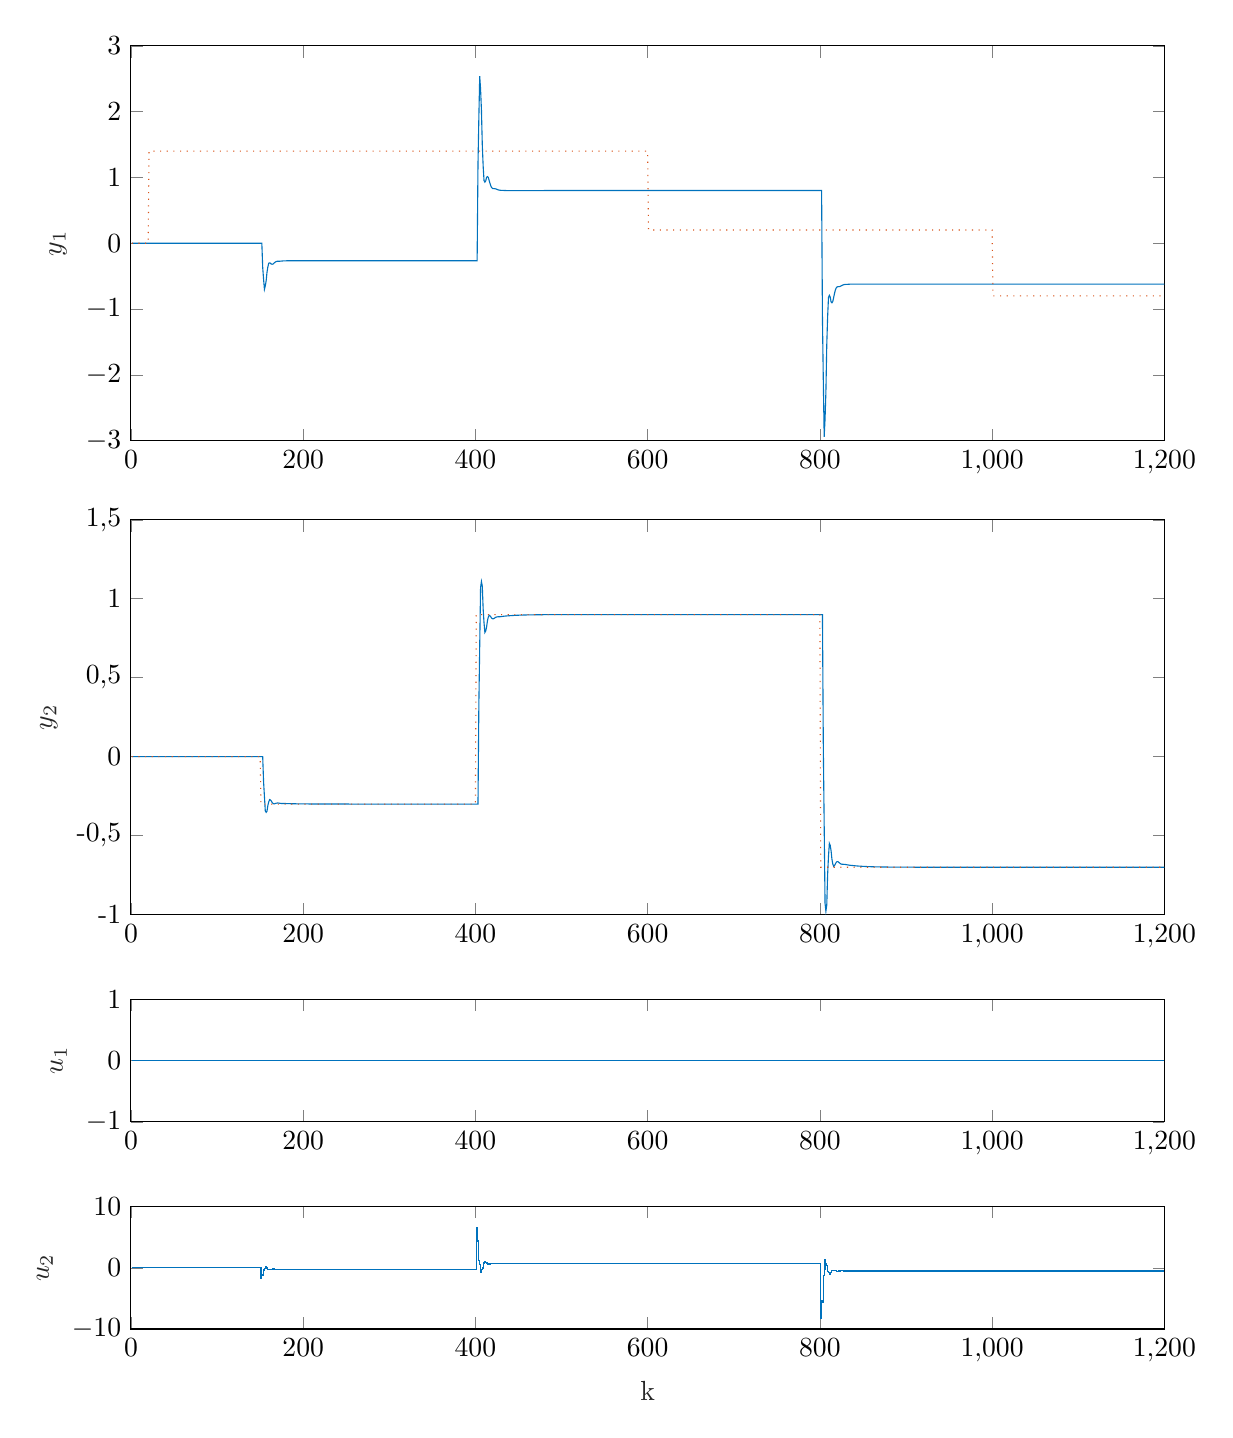
\begin{tikzpicture}

\begin{axis}[%
width=5.167in,
height=0.612in,
at={(0.646in,0.494in)},
scale only axis,
xmin=0,
xmax=1200,
xtick={0,200,400,600,800,1000,1200},
xlabel style={font=\color{white!15!black}},
xlabel={k},
ymin=-10,
ymax=10,
ytick={-10,0,10},
ylabel style={font=\color{white!15!black}},
ylabel={$\text{u}_\text{2}$},
axis background/.style={fill=white}
]
\addplot[const plot, color=mycolor1, forget plot] table[row sep=crcr] {%
1	0\\
2	0\\
3	0\\
4	0\\
5	0\\
6	0\\
7	0\\
8	0\\
9	0\\
10	0\\
11	0\\
12	0\\
13	0\\
14	0\\
15	0\\
16	0\\
17	0\\
18	0\\
19	0\\
20	0\\
21	0\\
22	0\\
23	0\\
24	0\\
25	0\\
26	0\\
27	0\\
28	0\\
29	0\\
30	0\\
31	0\\
32	0\\
33	0\\
34	0\\
35	0\\
36	0\\
37	0\\
38	0\\
39	0\\
40	0\\
41	0\\
42	0\\
43	0\\
44	0\\
45	0\\
46	0\\
47	0\\
48	0\\
49	0\\
50	0\\
51	0\\
52	0\\
53	0\\
54	0\\
55	0\\
56	0\\
57	0\\
58	0\\
59	0\\
60	0\\
61	0\\
62	0\\
63	0\\
64	0\\
65	0\\
66	0\\
67	0\\
68	0\\
69	0\\
70	0\\
71	0\\
72	0\\
73	0\\
74	0\\
75	0\\
76	0\\
77	0\\
78	0\\
79	0\\
80	0\\
81	0\\
82	0\\
83	0\\
84	0\\
85	0\\
86	0\\
87	0\\
88	0\\
89	0\\
90	0\\
91	0\\
92	0\\
93	0\\
94	0\\
95	0\\
96	0\\
97	0\\
98	0\\
99	0\\
100	0\\
101	0\\
102	0\\
103	0\\
104	0\\
105	0\\
106	0\\
107	0\\
108	0\\
109	0\\
110	0\\
111	0\\
112	0\\
113	0\\
114	0\\
115	0\\
116	0\\
117	0\\
118	0\\
119	0\\
120	0\\
121	0\\
122	0\\
123	0\\
124	0\\
125	0\\
126	0\\
127	0\\
128	0\\
129	0\\
130	0\\
131	0\\
132	0\\
133	0\\
134	0\\
135	0\\
136	0\\
137	0\\
138	0\\
139	0\\
140	0\\
141	0\\
142	0\\
143	0\\
144	0\\
145	0\\
146	0\\
147	0\\
148	0\\
149	0\\
150	0\\
151	-1.68475\\
152	-1.12125\\
153	-1.17875\\
154	-0.355736422736457\\
155	-0.182442463673081\\
156	0.133539883128637\\
157	0.00357569302754235\\
158	-0.0470778419975246\\
159	-0.226717837083248\\
160	-0.271530449802226\\
161	-0.315851479324673\\
162	-0.276118937023376\\
163	-0.250237591885371\\
164	-0.210736565716769\\
165	-0.201599296895201\\
166	-0.198009703778164\\
167	-0.209833467499791\\
168	-0.218219467293394\\
169	-0.226517536478594\\
170	-0.227810777596302\\
171	-0.227137127591581\\
172	-0.223866250182907\\
173	-0.221673212107589\\
174	-0.220139154816782\\
175	-0.220209143388749\\
176	-0.22076725083216\\
177	-0.221682144233814\\
178	-0.222245172306459\\
179	-0.222533216465584\\
180	-0.222462818103196\\
181	-0.222294979842552\\
182	-0.222102291338007\\
183	-0.222015674058359\\
184	-0.222010930569533\\
185	-0.222079612777202\\
186	-0.222159858301401\\
187	-0.222230046117523\\
188	-0.222268340149018\\
189	-0.222283805210331\\
190	-0.222284058478431\\
191	-0.222283619481432\\
192	-0.222287632189491\\
193	-0.222299059025489\\
194	-0.222314809004916\\
195	-0.22233212575071\\
196	-0.222347806661917\\
197	-0.222360924295141\\
198	-0.222371383592999\\
199	-0.222380211307956\\
200	-0.222388260708287\\
201	-0.222396243305188\\
202	-0.222404314343296\\
203	-0.222412399588285\\
204	-0.222420236571994\\
205	-0.222427638276309\\
206	-0.222434497918221\\
207	-0.222440838896641\\
208	-0.222446734788458\\
209	-0.222452281811276\\
210	-0.222457546572061\\
211	-0.222462566532152\\
212	-0.222467348526115\\
213	-0.222471888983632\\
214	-0.222476182977483\\
215	-0.22248023403212\\
216	-0.22248405294895\\
217	-0.222487656065605\\
218	-0.222491060276673\\
219	-0.222494280751021\\
220	-0.222497329360644\\
221	-0.2225002153866\\
222	-0.222502946400563\\
223	-0.222505529498202\\
224	-0.222507971835077\\
225	-0.22251028084741\\
226	-0.222512464013633\\
227	-0.222514528598686\\
228	-0.222516481402972\\
229	-0.222518328691022\\
230	-0.222520076212238\\
231	-0.222521729306177\\
232	-0.222523292997957\\
233	-0.222524772072245\\
234	-0.222526171100455\\
235	-0.222527494443945\\
236	-0.222528746242448\\
237	-0.222529930407754\\
238	-0.222531050625303\\
239	-0.222532110366192\\
240	-0.222533112903469\\
241	-0.222534061329411\\
242	-0.222534958569759\\
243	-0.222535807394661\\
244	-0.222536610426585\\
245	-0.222537370146844\\
246	-0.222538088901732\\
247	-0.222538768909039\\
248	-0.222539412264908\\
249	-0.222540020950834\\
250	-0.22254059684041\\
251	-0.222541141705602\\
252	-0.222541657222468\\
253	-0.222542144976373\\
254	-0.222542606466824\\
255	-0.222543043112033\\
256	-0.222543456253267\\
257	-0.222543847159026\\
258	-0.222544217029032\\
259	-0.222544566998006\\
260	-0.222544898139246\\
261	-0.222545211467978\\
262	-0.222545507944519\\
263	-0.222545788477253\\
264	-0.222546053925445\\
265	-0.2225463051019\\
266	-0.222546542775489\\
267	-0.22254676767353\\
268	-0.222546980484052\\
269	-0.222547181857923\\
270	-0.22254737241087\\
271	-0.222547552725381\\
272	-0.222547723352512\\
273	-0.222547884813582\\
274	-0.222548037601789\\
275	-0.222548182183729\\
276	-0.222548319000835\\
277	-0.222548448470741\\
278	-0.22254857098857\\
279	-0.222548686928149\\
280	-0.222548796643163\\
281	-0.22254890046824\\
282	-0.222548998719985\\
283	-0.222549091697952\\
284	-0.222549179685562\\
285	-0.222549262950981\\
286	-0.222549341747936\\
287	-0.222549416316498\\
288	-0.222549486883821\\
289	-0.222549553664832\\
290	-0.222549616862897\\
291	-0.222549676670443\\
292	-0.222549733269545\\
293	-0.222549786832489\\
294	-0.222549837522294\\
295	-0.222549885493215\\
296	-0.222549930891216\\
297	-0.222549973854411\\
298	-0.222550014513494\\
299	-0.222550052992133\\
300	-0.22255008940735\\
301	-0.222550123869882\\
302	-0.222550156484514\\
303	-0.222550187350403\\
304	-0.222550216561378\\
305	-0.222550244206231\\
306	-0.222550270368983\\
307	-0.222550295129144\\
308	-0.222550318561954\\
309	-0.222550340738613\\
310	-0.222550361726499\\
311	-0.222550381589373\\
312	-0.222550400387572\\
313	-0.222550418178194\\
314	-0.222550435015274\\
315	-0.222550450949947\\
316	-0.222550466030601\\
317	-0.222550480303031\\
318	-0.222550493810572\\
319	-0.222550506594235\\
320	-0.22255051869283\\
321	-0.222550530143086\\
322	-0.222550540979759\\
323	-0.222550551235744\\
324	-0.222550560942169\\
325	-0.222550570128494\\
326	-0.222550578822598\\
327	-0.222550587050864\\
328	-0.222550594838261\\
329	-0.22255060220842\\
330	-0.222550609183702\\
331	-0.222550615785272\\
332	-0.222550622033157\\
333	-0.222550627946313\\
334	-0.222550633542678\\
335	-0.222550638839228\\
336	-0.22255064385203\\
337	-0.22255064859629\\
338	-0.222550653086397\\
339	-0.22255065733597\\
340	-0.222550661357899\\
341	-0.222550665164379\\
342	-0.222550668766956\\
343	-0.222550672176554\\
344	-0.222550675403513\\
345	-0.222550678457619\\
346	-0.222550681348132\\
347	-0.222550684083817\\
348	-0.222550686672969\\
349	-0.222550689123438\\
350	-0.222550691442654\\
351	-0.22255069363765\\
352	-0.222550695715078\\
353	-0.222550697681238\\
354	-0.222550699542089\\
355	-0.222550701303274\\
356	-0.222550702970131\\
357	-0.222550704547713\\
358	-0.222550706040803\\
359	-0.222550707453925\\
360	-0.222550708791365\\
361	-0.222550710057175\\
362	-0.222550711255193\\
363	-0.222550712389049\\
364	-0.222550713462181\\
365	-0.222550714477841\\
366	-0.222550715439107\\
367	-0.222550716348892\\
368	-0.222550717209954\\
369	-0.222550718024903\\
370	-0.222550718796209\\
371	-0.222550719526209\\
372	-0.222550720217115\\
373	-0.222550720871021\\
374	-0.222550721489909\\
375	-0.222550722075654\\
376	-0.222550722630031\\
377	-0.22255072315472\\
378	-0.222550723651311\\
379	-0.222550724121309\\
380	-0.222550724566139\\
381	-0.222550724987147\\
382	-0.222550725385611\\
383	-0.222550725762736\\
384	-0.222550726119667\\
385	-0.222550726457483\\
386	-0.22255072677721\\
387	-0.222550727079816\\
388	-0.222550727366219\\
389	-0.222550727637284\\
390	-0.222550727893834\\
391	-0.222550728136646\\
392	-0.222550728366456\\
393	-0.222550728583959\\
394	-0.222550728789816\\
395	-0.222550728984649\\
396	-0.22255072916905\\
397	-0.222550729343577\\
398	-0.222550729508758\\
399	-0.222550729665095\\
400	-0.22255072981306\\
401	6.5164492700469\\
402	4.26244926991436\\
403	4.49244926978891\\
404	1.20039496061601\\
405	0.507219124250139\\
406	-0.75671026306309\\
407	-0.236853502759371\\
408	-0.034239362754372\\
409	0.684320617498353\\
410	0.863571068288927\\
411	1.04085518629795\\
412	0.881925017016312\\
413	0.778399636391943\\
414	0.620395531649057\\
415	0.583846456297976\\
416	0.569488083768488\\
417	0.616783138596938\\
418	0.650327137716405\\
419	0.683519414405196\\
420	0.688692378826809\\
421	0.685997778761337\\
422	0.672914269082552\\
423	0.664142116739549\\
424	0.658005887536828\\
425	0.658285841787316\\
426	0.660518271525581\\
427	0.66417784509871\\
428	0.666429957357599\\
429	0.667582133964105\\
430	0.667300540486165\\
431	0.666629187416719\\
432	0.665858433373112\\
433	0.665511964230453\\
434	0.665492990252366\\
435	0.665767719061482\\
436	0.666088701137872\\
437	0.666369452383045\\
438	0.66652262849074\\
439	0.666584488718691\\
440	0.666585501774718\\
441	0.666583745771225\\
442	0.666599796588794\\
443	0.666645503918906\\
444	0.666708503823474\\
445	0.666777770794217\\
446	0.666840494427273\\
447	0.666892964949027\\
448	0.666934802129912\\
449	0.666970112979764\\
450	0.66700231057164\\
451	0.667034240950309\\
452	0.667066525094278\\
453	0.667098866066227\\
454	0.667130213993483\\
455	0.667159820803572\\
456	0.66718725936443\\
457	0.667212623271688\\
458	0.667236206832878\\
459	0.667258394918395\\
460	0.667279453956084\\
461	0.667299533791292\\
462	0.667318661762265\\
463	0.667336823587717\\
464	0.66735399955875\\
465	0.667370203773163\\
466	0.667385479436573\\
467	0.667399891899485\\
468	0.667413508740252\\
469	0.66742639063432\\
470	0.667438585069673\\
471	0.667450129170522\\
472	0.667461053223563\\
473	0.667471385611454\\
474	0.667481154956437\\
475	0.66749039100338\\
476	0.667499123666016\\
477	0.667507382004089\\
478	0.667515193219211\\
479	0.667522582369493\\
480	0.667529572452548\\
481	0.667536184826587\\
482	0.667542439592084\\
483	0.6675483558877\\
484	0.667553951999087\\
485	0.667559245371668\\
486	0.667564252564377\\
487	0.667568989224363\\
488	0.667573470093392\\
489	0.667577709055844\\
490	0.66758171920391\\
491	0.667585512906692\\
492	0.667589101867145\\
493	0.66759249716587\\
494	0.667595709292726\\
495	0.667598748172967\\
496	0.667601623191769\\
497	0.667604343220287\\
498	0.667606916643089\\
499	0.667609351386157\\
500	0.667611654943856\\
501	0.667613834404054\\
502	0.667615896470977\\
503	0.667617847486088\\
504	0.667619693447413\\
505	0.667621440027791\\
506	0.667623092592293\\
507	0.667624656214919\\
508	0.667626135694551\\
509	0.667627535570081\\
510	0.667628860134692\\
511	0.66763011344929\\
512	0.667631299355142\\
513	0.667632421485784\\
514	0.667633483278272\\
515	0.66763448798383\\
516	0.667635438677937\\
517	0.667636338269869\\
518	0.667637189511733\\
519	0.667637995007003\\
520	0.667638757218584\\
521	0.667639478476437\\
522	0.667640160984778\\
523	0.667640806828889\\
524	0.667641417981556\\
525	0.667641996309163\\
526	0.667642543577444\\
527	0.667643061456936\\
528	0.667643551528125\\
529	0.667644015286322\\
530	0.66764445414626\\
531	0.667644869446459\\
532	0.667645262453337\\
533	0.667645634365105\\
534	0.667645986315458\\
535	0.667646319377046\\
536	0.667646634564783\\
537	0.667646932838955\\
538	0.667647215108167\\
539	0.667647482232139\\
540	0.667647735024333\\
541	0.667647974254454\\
542	0.667648200650805\\
543	0.667648414902524\\
544	0.667648617661693\\
545	0.66764880954533\\
546	0.667648991137284\\
547	0.667649162990019\\
548	0.667649325626304\\
549	0.667649479540815\\
550	0.667649625201644\\
551	0.667649763051734\\
552	0.667649893510226\\
553	0.667650016973746\\
554	0.667650133817615\\
555	0.667650244396997\\
556	0.667650349047978\\
557	0.667650448088597\\
558	0.667650541819813\\
559	0.667650630526427\\
560	0.667650714477949\\
561	0.667650793929421\\
562	0.667650869122194\\
563	0.667650940284663\\
564	0.667651007632965\\
565	0.667651071371635\\
566	0.667651131694235\\
567	0.667651188783937\\
568	0.667651242814084\\
569	0.66765129394872\\
570	0.667651342343088\\
571	0.667651388144099\\
572	0.667651431490784\\
573	0.667651472514715\\
574	0.667651511340406\\
575	0.667651548085697\\
576	0.667651582862102\\
577	0.667651615775157\\
578	0.667651646924739\\
579	0.667651676405366\\
580	0.667651704306489\\
581	0.667651730712761\\
582	0.667651755704296\\
583	0.667651779356913\\
584	0.667651801742368\\
585	0.667651822928563\\
586	0.667651842979768\\
587	0.667651861956802\\
588	0.667651879917227\\
589	0.667651896915517\\
590	0.667651913003227\\
591	0.667651928229147\\
592	0.667651942639452\\
593	0.667651956277842\\
594	0.667651969185676\\
595	0.667651981402095\\
596	0.667651992964144\\
597	0.667652003906881\\
598	0.667652014263485\\
599	0.66765202406536\\
600	0.667652033342222\\
601	0.667652042122198\\
602	0.667652050431909\\
603	0.667652058296546\\
604	0.667652065739952\\
605	0.667652072784689\\
606	0.667652079452114\\
607	0.667652085762441\\
608	0.667652091734796\\
609	0.667652097387286\\
610	0.667652102737042\\
611	0.667652107800282\\
612	0.667652112592352\\
613	0.667652117127777\\
614	0.667652121420304\\
615	0.667652125482942\\
616	0.667652129328004\\
617	0.667652132967145\\
618	0.667652136411394\\
619	0.66765213967119\\
620	0.667652142756411\\
621	0.667652145676409\\
622	0.667652148440031\\
623	0.667652151055653\\
624	0.667652153531202\\
625	0.667652155874181\\
626	0.667652158091688\\
627	0.667652160190445\\
628	0.667652162176811\\
629	0.667652164056804\\
630	0.667652165836121\\
631	0.667652167520156\\
632	0.667652169114009\\
633	0.667652170622513\\
634	0.667652172050235\\
635	0.667652173401503\\
636	0.66765217468041\\
637	0.667652175890832\\
638	0.667652177036438\\
639	0.667652178120698\\
640	0.667652179146897\\
641	0.667652180118144\\
642	0.667652181037383\\
643	0.667652181907398\\
644	0.667652182730826\\
645	0.667652183510162\\
646	0.667652184247766\\
647	0.667652184945872\\
648	0.667652185606597\\
649	0.667652186231941\\
650	0.667652186823799\\
651	0.667652187383965\\
652	0.667652187914136\\
653	0.667652188415919\\
654	0.667652188890832\\
655	0.667652189340316\\
656	0.667652189765732\\
657	0.667652190168368\\
658	0.667652190549446\\
659	0.667652190910117\\
660	0.667652191251476\\
661	0.667652191574556\\
662	0.667652191880337\\
663	0.667652192169745\\
664	0.667652192443655\\
665	0.667652192702899\\
666	0.667652192948261\\
667	0.667652193180485\\
668	0.667652193400274\\
669	0.667652193608295\\
670	0.667652193805178\\
671	0.667652193991519\\
672	0.667652194167883\\
673	0.667652194334805\\
674	0.667652194492788\\
675	0.667652194642312\\
676	0.667652194783829\\
677	0.66765219491777\\
678	0.667652195044538\\
679	0.667652195164518\\
680	0.667652195278074\\
681	0.667652195385549\\
682	0.66765219548727\\
683	0.667652195583545\\
684	0.667652195674664\\
685	0.667652195760905\\
686	0.667652195842528\\
687	0.66765219591978\\
688	0.667652195992895\\
689	0.667652196062095\\
690	0.667652196127589\\
691	0.667652196189578\\
692	0.667652196248247\\
693	0.667652196303776\\
694	0.667652196356332\\
695	0.667652196406074\\
696	0.667652196453152\\
697	0.66765219649771\\
698	0.667652196539881\\
699	0.667652196579795\\
700	0.66765219661757\\
701	0.667652196653323\\
702	0.667652196687162\\
703	0.66765219671919\\
704	0.667652196749502\\
705	0.667652196778191\\
706	0.667652196805344\\
707	0.667652196831043\\
708	0.667652196855366\\
709	0.667652196878387\\
710	0.667652196900175\\
711	0.667652196920797\\
712	0.667652196940314\\
713	0.667652196958787\\
714	0.667652196976271\\
715	0.667652196992818\\
716	0.66765219700848\\
717	0.667652197023303\\
718	0.667652197037332\\
719	0.66765219705061\\
720	0.667652197063176\\
721	0.667652197075071\\
722	0.667652197086327\\
723	0.667652197096982\\
724	0.667652197107066\\
725	0.667652197116611\\
726	0.667652197125644\\
727	0.667652197134193\\
728	0.667652197142284\\
729	0.667652197149943\\
730	0.667652197157192\\
731	0.667652197164053\\
732	0.667652197170546\\
733	0.667652197176693\\
734	0.667652197182509\\
735	0.667652197188015\\
736	0.667652197193225\\
737	0.667652197198156\\
738	0.667652197202822\\
739	0.667652197207238\\
740	0.667652197211417\\
741	0.667652197215374\\
742	0.667652197219118\\
743	0.667652197222664\\
744	0.667652197226019\\
745	0.667652197229194\\
746	0.667652197232199\\
747	0.667652197235045\\
748	0.667652197237737\\
749	0.667652197240285\\
750	0.667652197242696\\
751	0.667652197244978\\
752	0.667652197247139\\
753	0.667652197249184\\
754	0.66765219725112\\
755	0.667652197252951\\
756	0.667652197254683\\
757	0.667652197256322\\
758	0.667652197257874\\
759	0.667652197259344\\
760	0.667652197260735\\
761	0.66765219726205\\
762	0.667652197263296\\
763	0.667652197264476\\
764	0.667652197265593\\
765	0.667652197266651\\
766	0.667652197267651\\
767	0.667652197268597\\
768	0.667652197269492\\
769	0.667652197270338\\
770	0.66765219727114\\
771	0.667652197271898\\
772	0.667652197272616\\
773	0.667652197273296\\
774	0.667652197273939\\
775	0.667652197274548\\
776	0.667652197275125\\
777	0.66765219727567\\
778	0.667652197276186\\
779	0.667652197276674\\
780	0.667652197277137\\
781	0.667652197277574\\
782	0.667652197277988\\
783	0.66765219727838\\
784	0.667652197278752\\
785	0.667652197279103\\
786	0.667652197279436\\
787	0.667652197279751\\
788	0.66765219728005\\
789	0.667652197280333\\
790	0.667652197280601\\
791	0.667652197280854\\
792	0.667652197281093\\
793	0.667652197281319\\
794	0.667652197281532\\
795	0.667652197281735\\
796	0.667652197281927\\
797	0.667652197282108\\
798	0.66765219728228\\
799	0.667652197282443\\
800	0.667652197282598\\
801	-8.31768113605059\\
802	-5.31234780271711\\
803	-5.61901446938365\\
804	-1.22960872397797\\
805	-0.305374275639846\\
806	1.37986490730276\\
807	0.686722560097032\\
808	0.416570373296774\\
809	-0.541509600493655\\
810	-0.78051020166145\\
811	-1.01688902578108\\
812	-0.804982133507415\\
813	-0.666948292771317\\
814	-0.456276153205367\\
815	-0.407544052823609\\
816	-0.388399556199347\\
817	-0.451459629381298\\
818	-0.496184961613795\\
819	-0.540441330601472\\
820	-0.547338616562534\\
821	-0.543745816537305\\
822	-0.526301137024334\\
823	-0.514604933955923\\
824	-0.506423295071581\\
825	-0.506796567455368\\
826	-0.509773140486857\\
827	-0.514652571962306\\
828	-0.517655388349714\\
829	-0.519191623865018\\
830	-0.518816165932253\\
831	-0.517921028542122\\
832	-0.516893356517859\\
833	-0.516431397693049\\
834	-0.516406099085949\\
835	-0.516772404193495\\
836	-0.517200380322536\\
837	-0.517574715341831\\
838	-0.517778950176446\\
839	-0.517861430503431\\
840	-0.517862781266615\\
841	-0.517860439949273\\
842	-0.517881841058906\\
843	-0.517942784184218\\
844	-0.51802678407448\\
845	-0.518119140052038\\
846	-0.518202771578459\\
847	-0.518272732288972\\
848	-0.518328515210864\\
849	-0.518375596357294\\
850	-0.518418526492379\\
851	-0.518461100342513\\
852	-0.518504145879077\\
853	-0.518547267185678\\
854	-0.518589064432116\\
855	-0.518628540188456\\
856	-0.518665124945308\\
857	-0.518698943496876\\
858	-0.518730388253229\\
859	-0.518759972374919\\
860	-0.518788051099096\\
861	-0.518814824219578\\
862	-0.518840328187378\\
863	-0.518864543960801\\
864	-0.518887445261334\\
865	-0.518909050886062\\
866	-0.51892941844249\\
867	-0.518948635064642\\
868	-0.518966790857007\\
869	-0.518983966720187\\
870	-0.51900022597151\\
871	-0.519015618109936\\
872	-0.519030183517737\\
873	-0.519043960038472\\
874	-0.519056985835142\\
875	-0.519069300567579\\
876	-0.519080944120771\\
877	-0.519091955241047\\
878	-0.519102370197238\\
879	-0.519112222400164\\
880	-0.519121542513318\\
881	-0.519130359014321\\
882	-0.519138698703815\\
883	-0.519146587100017\\
884	-0.519154048583804\\
885	-0.519161106415747\\
886	-0.519167782674429\\
887	-0.519174098222722\\
888	-0.519180072716315\\
889	-0.51918572466772\\
890	-0.5191910715332\\
891	-0.519196129804891\\
892	-0.519200915086741\\
893	-0.519205442152888\\
894	-0.519209724989814\\
895	-0.519213776831193\\
896	-0.519217610190596\\
897	-0.519221236896234\\
898	-0.519224668127534\\
899	-0.519227914452473\\
900	-0.519230985863542\\
901	-0.519233891811233\\
902	-0.519236641234517\\
903	-0.519239242588678\\
904	-0.519241703871089\\
905	-0.519244032645539\\
906	-0.519246236065453\\
907	-0.519248320896169\\
908	-0.519250293536196\\
909	-0.519252160037392\\
910	-0.519253926124002\\
911	-0.519255597210571\\
912	-0.519257178418788\\
913	-0.519258674593369\\
914	-0.519260090317058\\
915	-0.519261429924822\\
916	-0.519262697517298\\
917	-0.519263896973524\\
918	-0.519265031962975\\
919	-0.519266105956949\\
920	-0.519267122239323\\
921	-0.519268083916713\\
922	-0.519268993928074\\
923	-0.519269855053782\\
924	-0.519270669924222\\
925	-0.5192714410279\\
926	-0.519272170719134\\
927	-0.519272861225303\\
928	-0.519273514653726\\
929	-0.519274132998149\\
930	-0.519274718144887\\
931	-0.519275271878632\\
932	-0.51927579588794\\
933	-0.519276291770429\\
934	-0.51927676103769\\
935	-0.519277205119925\\
936	-0.519277625370352\\
937	-0.519278023069352\\
938	-0.5192783994284\\
939	-0.519278755593788\\
940	-0.519279092650134\\
941	-0.519279411623709\\
942	-0.519279713485591\\
943	-0.519279999154625\\
944	-0.519280269500255\\
945	-0.519280525345171\\
946	-0.51928076746784\\
947	-0.519280996604881\\
948	-0.519281213453321\\
949	-0.519281418672726\\
950	-0.519281612887218\\
951	-0.519281796687386\\
952	-0.519281970632089\\
953	-0.519282135250159\\
954	-0.519282291042027\\
955	-0.519282438481242\\
956	-0.51928257801592\\
957	-0.519282710070112\\
958	-0.519282835045099\\
959	-0.519282953320615\\
960	-0.519283065256009\\
961	-0.519283171191334\\
962	-0.519283271448392\\
963	-0.519283366331709\\
964	-0.519283456129469\\
965	-0.519283541114385\\
966	-0.51928362154454\\
967	-0.519283697664163\\
968	-0.519283769704379\\
969	-0.519283837883912\\
970	-0.519283902409752\\
971	-0.519283963477781\\
972	-0.519284021273373\\
973	-0.519284075971961\\
974	-0.519284127739565\\
975	-0.519284176733299\\
976	-0.519284223101853\\
977	-0.519284266985939\\
978	-0.519284308518726\\
979	-0.519284347826238\\
980	-0.519284385027744\\
981	-0.519284420236114\\
982	-0.519284453558169\\
983	-0.519284485095001\\
984	-0.519284514942281\\
985	-0.51928454319055\\
986	-0.519284569925498\\
987	-0.519284595228219\\
988	-0.519284619175459\\
989	-0.519284641839851\\
990	-0.519284663290134\\
991	-0.519284683591364\\
992	-0.519284702805107\\
993	-0.519284720989631\\
994	-0.519284738200081\\
995	-0.519284754488646\\
996	-0.519284769904716\\
997	-0.519284784495037\\
998	-0.519284798303848\\
999	-0.519284811373017\\
1000	-0.519284823742171\\
1001	-0.519284835448811\\
1002	-0.519284846528428\\
1003	-0.519284857014612\\
1004	-0.519284866939155\\
1005	-0.51928487633214\\
1006	-0.519284885222043\\
1007	-0.519284893635814\\
1008	-0.519284901598957\\
1009	-0.519284909135611\\
1010	-0.519284916268622\\
1011	-0.519284923019609\\
1012	-0.519284929409038\\
1013	-0.519284935456272\\
1014	-0.519284941179642\\
1015	-0.519284946596494\\
1016	-0.519284951723246\\
1017	-0.519284956575435\\
1018	-0.519284961167769\\
1019	-0.519284965514166\\
1020	-0.519284969627797\\
1021	-0.519284973521129\\
1022	-0.519284977205961\\
1023	-0.519284980693459\\
1024	-0.519284983994194\\
1025	-0.519284987118167\\
1026	-0.519284990074844\\
1027	-0.519284992873187\\
1028	-0.519284995521673\\
1029	-0.51928499802833\\
1030	-0.519285000400754\\
1031	-0.519285002646133\\
1032	-0.519285004771272\\
1033	-0.519285006782609\\
1034	-0.519285008686238\\
1035	-0.519285010487928\\
1036	-0.519285012193139\\
1037	-0.519285013807036\\
1038	-0.51928501533451\\
1039	-0.519285016780189\\
1040	-0.519285018148455\\
1041	-0.519285019443453\\
1042	-0.519285020669105\\
1043	-0.519285021829127\\
1044	-0.519285022927031\\
1045	-0.519285023966145\\
1046	-0.519285024949617\\
1047	-0.519285025880425\\
1048	-0.519285026761391\\
1049	-0.519285027595183\\
1050	-0.519285028384328\\
1051	-0.519285029131217\\
1052	-0.519285029838112\\
1053	-0.519285030507156\\
1054	-0.519285031140374\\
1055	-0.519285031739686\\
1056	-0.519285032306906\\
1057	-0.519285032843753\\
1058	-0.519285033351854\\
1059	-0.519285033832749\\
1060	-0.519285034287894\\
1061	-0.519285034718669\\
1062	-0.519285035126378\\
1063	-0.519285035512255\\
1064	-0.51928503587747\\
1065	-0.519285036223129\\
1066	-0.519285036550279\\
1067	-0.519285036859912\\
1068	-0.519285037152966\\
1069	-0.519285037430327\\
1070	-0.519285037692839\\
1071	-0.519285037941293\\
1072	-0.519285038176445\\
1073	-0.519285038399005\\
1074	-0.519285038609649\\
1075	-0.519285038809013\\
1076	-0.519285038997703\\
1077	-0.519285039176289\\
1078	-0.519285039345314\\
1079	-0.519285039505287\\
1080	-0.519285039656695\\
1081	-0.519285039799994\\
1082	-0.51928503993562\\
1083	-0.519285040063985\\
1084	-0.519285040185477\\
1085	-0.519285040300465\\
1086	-0.519285040409295\\
1087	-0.519285040512299\\
1088	-0.519285040609788\\
1089	-0.519285040702056\\
1090	-0.519285040789384\\
1091	-0.519285040872035\\
1092	-0.519285040950261\\
1093	-0.519285041024299\\
1094	-0.519285041094372\\
1095	-0.519285041160693\\
1096	-0.519285041223463\\
1097	-0.519285041282872\\
1098	-0.5192850413391\\
1099	-0.519285041392318\\
1100	-0.519285041442687\\
1101	-0.519285041490357\\
1102	-0.519285041535476\\
1103	-0.519285041578179\\
1104	-0.519285041618596\\
1105	-0.51928504165685\\
1106	-0.519285041693055\\
1107	-0.519285041727321\\
1108	-0.519285041759753\\
1109	-0.519285041790448\\
1110	-0.519285041819498\\
1111	-0.519285041846994\\
1112	-0.519285041873019\\
1113	-0.51928504189765\\
1114	-0.519285041920962\\
1115	-0.519285041943025\\
1116	-0.519285041963906\\
1117	-0.519285041983671\\
1118	-0.519285042002377\\
1119	-0.519285042020082\\
1120	-0.519285042036838\\
1121	-0.519285042052698\\
1122	-0.519285042067706\\
1123	-0.519285042081911\\
1124	-0.519285042095356\\
1125	-0.519285042108082\\
1126	-0.519285042120127\\
1127	-0.519285042131526\\
1128	-0.519285042142315\\
1129	-0.519285042152526\\
1130	-0.519285042162191\\
1131	-0.519285042171339\\
1132	-0.519285042179996\\
1133	-0.51928504218819\\
1134	-0.519285042195945\\
1135	-0.519285042203285\\
1136	-0.519285042210232\\
1137	-0.519285042216806\\
1138	-0.51928504222303\\
1139	-0.519285042228919\\
1140	-0.519285042234493\\
1141	-0.51928504223977\\
1142	-0.519285042244764\\
1143	-0.51928504224949\\
1144	-0.519285042253963\\
1145	-0.519285042258195\\
1146	-0.519285042262201\\
1147	-0.519285042265992\\
1148	-0.519285042269582\\
1149	-0.51928504227298\\
1150	-0.519285042276197\\
1151	-0.519285042279241\\
1152	-0.519285042282121\\
1153	-0.519285042284846\\
1154	-0.519285042287425\\
1155	-0.519285042289866\\
1156	-0.519285042292178\\
1157	-0.519285042294366\\
1158	-0.519285042296437\\
1159	-0.519285042298397\\
1160	-0.519285042300251\\
1161	-0.519285042302006\\
1162	-0.519285042303668\\
1163	-0.51928504230524\\
1164	-0.519285042306728\\
1165	-0.519285042308136\\
1166	-0.519285042309468\\
1167	-0.51928504231073\\
1168	-0.519285042311923\\
1169	-0.519285042313053\\
1170	-0.519285042314121\\
1171	-0.519285042315133\\
1172	-0.519285042316091\\
1173	-0.519285042316998\\
1174	-0.519285042317857\\
1175	-0.519285042318669\\
1176	-0.519285042319439\\
1177	-0.519285042320166\\
1178	-0.519285042320854\\
1179	-0.519285042321505\\
1180	-0.519285042322122\\
1181	-0.519285042322705\\
1182	-0.519285042323257\\
1183	-0.51928504232378\\
1184	-0.519285042324275\\
1185	-0.519285042324744\\
1186	-0.519285042325188\\
1187	-0.519285042325608\\
1188	-0.519285042326007\\
1189	-0.519285042326384\\
1190	-0.519285042326741\\
1191	-0.519285042327078\\
1192	-0.519285042327396\\
1193	-0.519285042327697\\
1194	-0.519285042327981\\
1195	-0.519285042328251\\
1196	-0.519285042328506\\
1197	-0.519285042328749\\
1198	-0.519285042328977\\
1199	-0.519285042329194\\
1200	-0.519285042329399\\
};
\end{axis}

\begin{axis}[%
width=5.167in,
height=0.612in,
at={(0.646in,1.53in)},
scale only axis,
xmin=0,
xmax=1200,
xtick={0,200,400,600,800,1000,1200},
ymin=-1,
ymax=1,
ytick={-1,0,1},
ylabel style={font=\color{white!15!black}},
ylabel={$\text{u}_\text{1}$},
axis background/.style={fill=white}
]
\addplot[const plot, color=mycolor1, forget plot] table[row sep=crcr] {%
1	0\\
2	0\\
3	0\\
4	0\\
5	0\\
6	0\\
7	0\\
8	0\\
9	0\\
10	0\\
11	0\\
12	0\\
13	0\\
14	0\\
15	0\\
16	0\\
17	0\\
18	0\\
19	0\\
20	0\\
21	0\\
22	0\\
23	0\\
24	0\\
25	0\\
26	0\\
27	0\\
28	0\\
29	0\\
30	0\\
31	0\\
32	0\\
33	0\\
34	0\\
35	0\\
36	0\\
37	0\\
38	0\\
39	0\\
40	0\\
41	0\\
42	0\\
43	0\\
44	0\\
45	0\\
46	0\\
47	0\\
48	0\\
49	0\\
50	0\\
51	0\\
52	0\\
53	0\\
54	0\\
55	0\\
56	0\\
57	0\\
58	0\\
59	0\\
60	0\\
61	0\\
62	0\\
63	0\\
64	0\\
65	0\\
66	0\\
67	0\\
68	0\\
69	0\\
70	0\\
71	0\\
72	0\\
73	0\\
74	0\\
75	0\\
76	0\\
77	0\\
78	0\\
79	0\\
80	0\\
81	0\\
82	0\\
83	0\\
84	0\\
85	0\\
86	0\\
87	0\\
88	0\\
89	0\\
90	0\\
91	0\\
92	0\\
93	0\\
94	0\\
95	0\\
96	0\\
97	0\\
98	0\\
99	0\\
100	0\\
101	0\\
102	0\\
103	0\\
104	0\\
105	0\\
106	0\\
107	0\\
108	0\\
109	0\\
110	0\\
111	0\\
112	0\\
113	0\\
114	0\\
115	0\\
116	0\\
117	0\\
118	0\\
119	0\\
120	0\\
121	0\\
122	0\\
123	0\\
124	0\\
125	0\\
126	0\\
127	0\\
128	0\\
129	0\\
130	0\\
131	0\\
132	0\\
133	0\\
134	0\\
135	0\\
136	0\\
137	0\\
138	0\\
139	0\\
140	0\\
141	0\\
142	0\\
143	0\\
144	0\\
145	0\\
146	0\\
147	0\\
148	0\\
149	0\\
150	0\\
151	0\\
152	0\\
153	0\\
154	0\\
155	0\\
156	0\\
157	0\\
158	0\\
159	0\\
160	0\\
161	0\\
162	0\\
163	0\\
164	0\\
165	0\\
166	0\\
167	0\\
168	0\\
169	0\\
170	0\\
171	0\\
172	0\\
173	0\\
174	0\\
175	0\\
176	0\\
177	0\\
178	0\\
179	0\\
180	0\\
181	0\\
182	0\\
183	0\\
184	0\\
185	0\\
186	0\\
187	0\\
188	0\\
189	0\\
190	0\\
191	0\\
192	0\\
193	0\\
194	0\\
195	0\\
196	0\\
197	0\\
198	0\\
199	0\\
200	0\\
201	0\\
202	0\\
203	0\\
204	0\\
205	0\\
206	0\\
207	0\\
208	0\\
209	0\\
210	0\\
211	0\\
212	0\\
213	0\\
214	0\\
215	0\\
216	0\\
217	0\\
218	0\\
219	0\\
220	0\\
221	0\\
222	0\\
223	0\\
224	0\\
225	0\\
226	0\\
227	0\\
228	0\\
229	0\\
230	0\\
231	0\\
232	0\\
233	0\\
234	0\\
235	0\\
236	0\\
237	0\\
238	0\\
239	0\\
240	0\\
241	0\\
242	0\\
243	0\\
244	0\\
245	0\\
246	0\\
247	0\\
248	0\\
249	0\\
250	0\\
251	0\\
252	0\\
253	0\\
254	0\\
255	0\\
256	0\\
257	0\\
258	0\\
259	0\\
260	0\\
261	0\\
262	0\\
263	0\\
264	0\\
265	0\\
266	0\\
267	0\\
268	0\\
269	0\\
270	0\\
271	0\\
272	0\\
273	0\\
274	0\\
275	0\\
276	0\\
277	0\\
278	0\\
279	0\\
280	0\\
281	0\\
282	0\\
283	0\\
284	0\\
285	0\\
286	0\\
287	0\\
288	0\\
289	0\\
290	0\\
291	0\\
292	0\\
293	0\\
294	0\\
295	0\\
296	0\\
297	0\\
298	0\\
299	0\\
300	0\\
301	0\\
302	0\\
303	0\\
304	0\\
305	0\\
306	0\\
307	0\\
308	0\\
309	0\\
310	0\\
311	0\\
312	0\\
313	0\\
314	0\\
315	0\\
316	0\\
317	0\\
318	0\\
319	0\\
320	0\\
321	0\\
322	0\\
323	0\\
324	0\\
325	0\\
326	0\\
327	0\\
328	0\\
329	0\\
330	0\\
331	0\\
332	0\\
333	0\\
334	0\\
335	0\\
336	0\\
337	0\\
338	0\\
339	0\\
340	0\\
341	0\\
342	0\\
343	0\\
344	0\\
345	0\\
346	0\\
347	0\\
348	0\\
349	0\\
350	0\\
351	0\\
352	0\\
353	0\\
354	0\\
355	0\\
356	0\\
357	0\\
358	0\\
359	0\\
360	0\\
361	0\\
362	0\\
363	0\\
364	0\\
365	0\\
366	0\\
367	0\\
368	0\\
369	0\\
370	0\\
371	0\\
372	0\\
373	0\\
374	0\\
375	0\\
376	0\\
377	0\\
378	0\\
379	0\\
380	0\\
381	0\\
382	0\\
383	0\\
384	0\\
385	0\\
386	0\\
387	0\\
388	0\\
389	0\\
390	0\\
391	0\\
392	0\\
393	0\\
394	0\\
395	0\\
396	0\\
397	0\\
398	0\\
399	0\\
400	0\\
401	0\\
402	0\\
403	0\\
404	0\\
405	0\\
406	0\\
407	0\\
408	0\\
409	0\\
410	0\\
411	0\\
412	0\\
413	0\\
414	0\\
415	0\\
416	0\\
417	0\\
418	0\\
419	0\\
420	0\\
421	0\\
422	0\\
423	0\\
424	0\\
425	0\\
426	0\\
427	0\\
428	0\\
429	0\\
430	0\\
431	0\\
432	0\\
433	0\\
434	0\\
435	0\\
436	0\\
437	0\\
438	0\\
439	0\\
440	0\\
441	0\\
442	0\\
443	0\\
444	0\\
445	0\\
446	0\\
447	0\\
448	0\\
449	0\\
450	0\\
451	0\\
452	0\\
453	0\\
454	0\\
455	0\\
456	0\\
457	0\\
458	0\\
459	0\\
460	0\\
461	0\\
462	0\\
463	0\\
464	0\\
465	0\\
466	0\\
467	0\\
468	0\\
469	0\\
470	0\\
471	0\\
472	0\\
473	0\\
474	0\\
475	0\\
476	0\\
477	0\\
478	0\\
479	0\\
480	0\\
481	0\\
482	0\\
483	0\\
484	0\\
485	0\\
486	0\\
487	0\\
488	0\\
489	0\\
490	0\\
491	0\\
492	0\\
493	0\\
494	0\\
495	0\\
496	0\\
497	0\\
498	0\\
499	0\\
500	0\\
501	0\\
502	0\\
503	0\\
504	0\\
505	0\\
506	0\\
507	0\\
508	0\\
509	0\\
510	0\\
511	0\\
512	0\\
513	0\\
514	0\\
515	0\\
516	0\\
517	0\\
518	0\\
519	0\\
520	0\\
521	0\\
522	0\\
523	0\\
524	0\\
525	0\\
526	0\\
527	0\\
528	0\\
529	0\\
530	0\\
531	0\\
532	0\\
533	0\\
534	0\\
535	0\\
536	0\\
537	0\\
538	0\\
539	0\\
540	0\\
541	0\\
542	0\\
543	0\\
544	0\\
545	0\\
546	0\\
547	0\\
548	0\\
549	0\\
550	0\\
551	0\\
552	0\\
553	0\\
554	0\\
555	0\\
556	0\\
557	0\\
558	0\\
559	0\\
560	0\\
561	0\\
562	0\\
563	0\\
564	0\\
565	0\\
566	0\\
567	0\\
568	0\\
569	0\\
570	0\\
571	0\\
572	0\\
573	0\\
574	0\\
575	0\\
576	0\\
577	0\\
578	0\\
579	0\\
580	0\\
581	0\\
582	0\\
583	0\\
584	0\\
585	0\\
586	0\\
587	0\\
588	0\\
589	0\\
590	0\\
591	0\\
592	0\\
593	0\\
594	0\\
595	0\\
596	0\\
597	0\\
598	0\\
599	0\\
600	0\\
601	0\\
602	0\\
603	0\\
604	0\\
605	0\\
606	0\\
607	0\\
608	0\\
609	0\\
610	0\\
611	0\\
612	0\\
613	0\\
614	0\\
615	0\\
616	0\\
617	0\\
618	0\\
619	0\\
620	0\\
621	0\\
622	0\\
623	0\\
624	0\\
625	0\\
626	0\\
627	0\\
628	0\\
629	0\\
630	0\\
631	0\\
632	0\\
633	0\\
634	0\\
635	0\\
636	0\\
637	0\\
638	0\\
639	0\\
640	0\\
641	0\\
642	0\\
643	0\\
644	0\\
645	0\\
646	0\\
647	0\\
648	0\\
649	0\\
650	0\\
651	0\\
652	0\\
653	0\\
654	0\\
655	0\\
656	0\\
657	0\\
658	0\\
659	0\\
660	0\\
661	0\\
662	0\\
663	0\\
664	0\\
665	0\\
666	0\\
667	0\\
668	0\\
669	0\\
670	0\\
671	0\\
672	0\\
673	0\\
674	0\\
675	0\\
676	0\\
677	0\\
678	0\\
679	0\\
680	0\\
681	0\\
682	0\\
683	0\\
684	0\\
685	0\\
686	0\\
687	0\\
688	0\\
689	0\\
690	0\\
691	0\\
692	0\\
693	0\\
694	0\\
695	0\\
696	0\\
697	0\\
698	0\\
699	0\\
700	0\\
701	0\\
702	0\\
703	0\\
704	0\\
705	0\\
706	0\\
707	0\\
708	0\\
709	0\\
710	0\\
711	0\\
712	0\\
713	0\\
714	0\\
715	0\\
716	0\\
717	0\\
718	0\\
719	0\\
720	0\\
721	0\\
722	0\\
723	0\\
724	0\\
725	0\\
726	0\\
727	0\\
728	0\\
729	0\\
730	0\\
731	0\\
732	0\\
733	0\\
734	0\\
735	0\\
736	0\\
737	0\\
738	0\\
739	0\\
740	0\\
741	0\\
742	0\\
743	0\\
744	0\\
745	0\\
746	0\\
747	0\\
748	0\\
749	0\\
750	0\\
751	0\\
752	0\\
753	0\\
754	0\\
755	0\\
756	0\\
757	0\\
758	0\\
759	0\\
760	0\\
761	0\\
762	0\\
763	0\\
764	0\\
765	0\\
766	0\\
767	0\\
768	0\\
769	0\\
770	0\\
771	0\\
772	0\\
773	0\\
774	0\\
775	0\\
776	0\\
777	0\\
778	0\\
779	0\\
780	0\\
781	0\\
782	0\\
783	0\\
784	0\\
785	0\\
786	0\\
787	0\\
788	0\\
789	0\\
790	0\\
791	0\\
792	0\\
793	0\\
794	0\\
795	0\\
796	0\\
797	0\\
798	0\\
799	0\\
800	0\\
801	0\\
802	0\\
803	0\\
804	0\\
805	0\\
806	0\\
807	0\\
808	0\\
809	0\\
810	0\\
811	0\\
812	0\\
813	0\\
814	0\\
815	0\\
816	0\\
817	0\\
818	0\\
819	0\\
820	0\\
821	0\\
822	0\\
823	0\\
824	0\\
825	0\\
826	0\\
827	0\\
828	0\\
829	0\\
830	0\\
831	0\\
832	0\\
833	0\\
834	0\\
835	0\\
836	0\\
837	0\\
838	0\\
839	0\\
840	0\\
841	0\\
842	0\\
843	0\\
844	0\\
845	0\\
846	0\\
847	0\\
848	0\\
849	0\\
850	0\\
851	0\\
852	0\\
853	0\\
854	0\\
855	0\\
856	0\\
857	0\\
858	0\\
859	0\\
860	0\\
861	0\\
862	0\\
863	0\\
864	0\\
865	0\\
866	0\\
867	0\\
868	0\\
869	0\\
870	0\\
871	0\\
872	0\\
873	0\\
874	0\\
875	0\\
876	0\\
877	0\\
878	0\\
879	0\\
880	0\\
881	0\\
882	0\\
883	0\\
884	0\\
885	0\\
886	0\\
887	0\\
888	0\\
889	0\\
890	0\\
891	0\\
892	0\\
893	0\\
894	0\\
895	0\\
896	0\\
897	0\\
898	0\\
899	0\\
900	0\\
901	0\\
902	0\\
903	0\\
904	0\\
905	0\\
906	0\\
907	0\\
908	0\\
909	0\\
910	0\\
911	0\\
912	0\\
913	0\\
914	0\\
915	0\\
916	0\\
917	0\\
918	0\\
919	0\\
920	0\\
921	0\\
922	0\\
923	0\\
924	0\\
925	0\\
926	0\\
927	0\\
928	0\\
929	0\\
930	0\\
931	0\\
932	0\\
933	0\\
934	0\\
935	0\\
936	0\\
937	0\\
938	0\\
939	0\\
940	0\\
941	0\\
942	0\\
943	0\\
944	0\\
945	0\\
946	0\\
947	0\\
948	0\\
949	0\\
950	0\\
951	0\\
952	0\\
953	0\\
954	0\\
955	0\\
956	0\\
957	0\\
958	0\\
959	0\\
960	0\\
961	0\\
962	0\\
963	0\\
964	0\\
965	0\\
966	0\\
967	0\\
968	0\\
969	0\\
970	0\\
971	0\\
972	0\\
973	0\\
974	0\\
975	0\\
976	0\\
977	0\\
978	0\\
979	0\\
980	0\\
981	0\\
982	0\\
983	0\\
984	0\\
985	0\\
986	0\\
987	0\\
988	0\\
989	0\\
990	0\\
991	0\\
992	0\\
993	0\\
994	0\\
995	0\\
996	0\\
997	0\\
998	0\\
999	0\\
1000	0\\
1001	0\\
1002	0\\
1003	0\\
1004	0\\
1005	0\\
1006	0\\
1007	0\\
1008	0\\
1009	0\\
1010	0\\
1011	0\\
1012	0\\
1013	0\\
1014	0\\
1015	0\\
1016	0\\
1017	0\\
1018	0\\
1019	0\\
1020	0\\
1021	0\\
1022	0\\
1023	0\\
1024	0\\
1025	0\\
1026	0\\
1027	0\\
1028	0\\
1029	0\\
1030	0\\
1031	0\\
1032	0\\
1033	0\\
1034	0\\
1035	0\\
1036	0\\
1037	0\\
1038	0\\
1039	0\\
1040	0\\
1041	0\\
1042	0\\
1043	0\\
1044	0\\
1045	0\\
1046	0\\
1047	0\\
1048	0\\
1049	0\\
1050	0\\
1051	0\\
1052	0\\
1053	0\\
1054	0\\
1055	0\\
1056	0\\
1057	0\\
1058	0\\
1059	0\\
1060	0\\
1061	0\\
1062	0\\
1063	0\\
1064	0\\
1065	0\\
1066	0\\
1067	0\\
1068	0\\
1069	0\\
1070	0\\
1071	0\\
1072	0\\
1073	0\\
1074	0\\
1075	0\\
1076	0\\
1077	0\\
1078	0\\
1079	0\\
1080	0\\
1081	0\\
1082	0\\
1083	0\\
1084	0\\
1085	0\\
1086	0\\
1087	0\\
1088	0\\
1089	0\\
1090	0\\
1091	0\\
1092	0\\
1093	0\\
1094	0\\
1095	0\\
1096	0\\
1097	0\\
1098	0\\
1099	0\\
1100	0\\
1101	0\\
1102	0\\
1103	0\\
1104	0\\
1105	0\\
1106	0\\
1107	0\\
1108	0\\
1109	0\\
1110	0\\
1111	0\\
1112	0\\
1113	0\\
1114	0\\
1115	0\\
1116	0\\
1117	0\\
1118	0\\
1119	0\\
1120	0\\
1121	0\\
1122	0\\
1123	0\\
1124	0\\
1125	0\\
1126	0\\
1127	0\\
1128	0\\
1129	0\\
1130	0\\
1131	0\\
1132	0\\
1133	0\\
1134	0\\
1135	0\\
1136	0\\
1137	0\\
1138	0\\
1139	0\\
1140	0\\
1141	0\\
1142	0\\
1143	0\\
1144	0\\
1145	0\\
1146	0\\
1147	0\\
1148	0\\
1149	0\\
1150	0\\
1151	0\\
1152	0\\
1153	0\\
1154	0\\
1155	0\\
1156	0\\
1157	0\\
1158	0\\
1159	0\\
1160	0\\
1161	0\\
1162	0\\
1163	0\\
1164	0\\
1165	0\\
1166	0\\
1167	0\\
1168	0\\
1169	0\\
1170	0\\
1171	0\\
1172	0\\
1173	0\\
1174	0\\
1175	0\\
1176	0\\
1177	0\\
1178	0\\
1179	0\\
1180	0\\
1181	0\\
1182	0\\
1183	0\\
1184	0\\
1185	0\\
1186	0\\
1187	0\\
1188	0\\
1189	0\\
1190	0\\
1191	0\\
1192	0\\
1193	0\\
1194	0\\
1195	0\\
1196	0\\
1197	0\\
1198	0\\
1199	0\\
1200	0\\
};
\end{axis}

\begin{axis}[%
width=5.167in,
height=1.974in,
at={(0.646in,2.566in)},
scale only axis,
xmin=0,
xmax=1200,
xtick={0,200,400,600,800,1000,1200},
ymin=-1,
ymax=1.5,
ytick={-1,-0.5,0,0.5,1,1.5},
yticklabels={{-1},{-0,5},{0},{0,5},{1},{1,5}},
ylabel style={font=\color{white!15!black}},
ylabel={$\text{y}_\text{2}$},
axis background/.style={fill=white}
]
\addplot [color=mycolor1, forget plot]
  table[row sep=crcr]{%
1	0\\
2	0\\
3	0\\
4	0\\
5	0\\
6	0\\
7	0\\
8	0\\
9	0\\
10	0\\
11	0\\
12	0\\
13	0\\
14	0\\
15	0\\
16	0\\
17	0\\
18	0\\
19	0\\
20	0\\
21	0\\
22	0\\
23	0\\
24	0\\
25	0\\
26	0\\
27	0\\
28	0\\
29	0\\
30	0\\
31	0\\
32	0\\
33	0\\
34	0\\
35	0\\
36	0\\
37	0\\
38	0\\
39	0\\
40	0\\
41	0\\
42	0\\
43	0\\
44	0\\
45	0\\
46	0\\
47	0\\
48	0\\
49	0\\
50	0\\
51	0\\
52	0\\
53	0\\
54	0\\
55	0\\
56	0\\
57	0\\
58	0\\
59	0\\
60	0\\
61	0\\
62	0\\
63	0\\
64	0\\
65	0\\
66	0\\
67	0\\
68	0\\
69	0\\
70	0\\
71	0\\
72	0\\
73	0\\
74	0\\
75	0\\
76	0\\
77	0\\
78	0\\
79	0\\
80	0\\
81	0\\
82	0\\
83	0\\
84	0\\
85	0\\
86	0\\
87	0\\
88	0\\
89	0\\
90	0\\
91	0\\
92	0\\
93	0\\
94	0\\
95	0\\
96	0\\
97	0\\
98	0\\
99	0\\
100	0\\
101	0\\
102	0\\
103	0\\
104	0\\
105	0\\
106	0\\
107	0\\
108	0\\
109	0\\
110	0\\
111	0\\
112	0\\
113	0\\
114	0\\
115	0\\
116	0\\
117	0\\
118	0\\
119	0\\
120	0\\
121	0\\
122	0\\
123	0\\
124	0\\
125	0\\
126	0\\
127	0\\
128	0\\
129	0\\
130	0\\
131	0\\
132	0\\
133	0\\
134	0\\
135	0\\
136	0\\
137	0\\
138	0\\
139	0\\
140	0\\
141	0\\
142	0\\
143	0\\
144	0\\
145	0\\
146	0\\
147	0\\
148	0\\
149	0\\
150	0\\
151	0\\
152	0\\
153	0\\
154	-0.15679125875\\
155	-0.250330396322125\\
156	-0.34277052731146\\
157	-0.352241819190754\\
158	-0.344930174819811\\
159	-0.308713516720857\\
160	-0.28708695152923\\
161	-0.271663947787628\\
162	-0.274021211695665\\
163	-0.280385387244436\\
164	-0.290434534654919\\
165	-0.296092178486777\\
166	-0.298950154145899\\
167	-0.297934003324969\\
168	-0.296136683373009\\
169	-0.294128423548302\\
170	-0.293358287895841\\
171	-0.293421050446503\\
172	-0.294251160769037\\
173	-0.295143855939638\\
174	-0.295911809150296\\
175	-0.29632194320347\\
176	-0.296499268788749\\
177	-0.296521196797421\\
178	-0.296547752699329\\
179	-0.296624073926298\\
180	-0.296779960995538\\
181	-0.296977206634919\\
182	-0.297187390170703\\
183	-0.297376281237508\\
184	-0.297536297992503\\
185	-0.297667135569581\\
186	-0.297780693179229\\
187	-0.297885796650337\\
188	-0.297989876032272\\
189	-0.298094090845112\\
190	-0.29819750749135\\
191	-0.2982972236247\\
192	-0.298391379759422\\
193	-0.298478952736241\\
194	-0.298560340504422\\
195	-0.298636391670053\\
196	-0.298708171447152\\
197	-0.298776383403466\\
198	-0.298841425569849\\
199	-0.298903370012984\\
200	-0.298962197081297\\
201	-0.299017879228902\\
202	-0.299070485993448\\
203	-0.299120161187193\\
204	-0.299167104610217\\
205	-0.299211516445395\\
206	-0.29925357589722\\
207	-0.299293425140115\\
208	-0.299331178911734\\
209	-0.299366933888974\\
210	-0.299400782064677\\
211	-0.299432815755352\\
212	-0.299463129699728\\
213	-0.299491818148737\\
214	-0.299518972198375\\
215	-0.299544677167674\\
216	-0.299569012038572\\
217	-0.299592049775692\\
218	-0.299613858536237\\
219	-0.299634502686503\\
220	-0.299654043585719\\
221	-0.2996725398519\\
222	-0.299690047396417\\
223	-0.299706619309496\\
224	-0.299722305818867\\
225	-0.299737154332911\\
226	-0.299751209595241\\
227	-0.299764513878171\\
228	-0.299777107183064\\
229	-0.299789027404401\\
230	-0.299800310458463\\
231	-0.299810990379538\\
232	-0.299821099402615\\
233	-0.299830668042113\\
234	-0.29983972517477\\
235	-0.299848298125524\\
236	-0.299856412754193\\
237	-0.29986409353855\\
238	-0.299871363651834\\
239	-0.299878245033702\\
240	-0.299884758455586\\
241	-0.299890923581575\\
242	-0.299896759026119\\
243	-0.299902282409166\\
244	-0.299907510409029\\
245	-0.299912458812838\\
246	-0.299917142564469\\
247	-0.299921575809826\\
248	-0.299925771939543\\
249	-0.299929743629261\\
250	-0.299933502877671\\
251	-0.299937061042526\\
252	-0.299940428874768\\
253	-0.299943616550893\\
254	-0.299946633703623\\
255	-0.299949489450959\\
256	-0.299952192423682\\
257	-0.299954750791376\\
258	-0.299957172287047\\
259	-0.29995946423043\\
260	-0.299961633550043\\
261	-0.299963686804077\\
262	-0.299965630200164\\
263	-0.299967469614107\\
264	-0.299969210607602\\
265	-0.299970858445018\\
266	-0.299972418109283\\
267	-0.299973894316917\\
268	-0.299975291532268\\
269	-0.299976613980979\\
270	-0.299977865662747\\
271	-0.299979050363395\\
272	-0.299980171666299\\
273	-0.29998123296321\\
274	-0.299982237464492\\
275	-0.29998318820882\\
276	-0.299984088072353\\
277	-0.299984939777427\\
278	-0.299985745900768\\
279	-0.299986508881286\\
280	-0.299987231027435\\
281	-0.299987914524189\\
282	-0.299988561439649\\
283	-0.299989173731283\\
284	-0.299989753251848\\
285	-0.299990301754988\\
286	-0.299990820900529\\
287	-0.299991312259504\\
288	-0.299991777318893\\
289	-0.299992217486122\\
290	-0.299992634093321\\
291	-0.299993028401344\\
292	-0.299993401603584\\
293	-0.299993754829583\\
294	-0.299994089148445\\
295	-0.299994405572069\\
296	-0.299994705058211\\
297	-0.299994988513375\\
298	-0.299995256795561\\
299	-0.299995510716856\\
300	-0.29999575104589\\
301	-0.299995978510161\\
302	-0.299996193798239\\
303	-0.299996397561842\\
304	-0.299996590417815\\
305	-0.299996772949988\\
306	-0.299996945710949\\
307	-0.299997109223713\\
308	-0.299997263983303\\
309	-0.299997410458251\\
310	-0.299997549092011\\
311	-0.299997680304305\\
312	-0.299997804492391\\
313	-0.299997922032264\\
314	-0.299998033279798\\
315	-0.299998138571816\\
316	-0.299998238227117\\
317	-0.299998332547434\\
318	-0.29999842181835\\
319	-0.299998506310165\\
320	-0.299998586278709\\
321	-0.299998661966119\\
322	-0.29999873360157\\
323	-0.299998801401974\\
324	-0.299998865572628\\
325	-0.299998926307843\\
326	-0.299998983791526\\
327	-0.299999038197744\\
328	-0.299999089691242\\
329	-0.29999913842795\\
330	-0.299999184555449\\
331	-0.299999228213421\\
332	-0.299999269534069\\
333	-0.299999308642523\\
334	-0.299999345657211\\
335	-0.299999380690222\\
336	-0.299999413847647\\
337	-0.299999445229896\\
338	-0.299999474932003\\
339	-0.299999503043917\\
340	-0.299999529650769\\
341	-0.299999554833136\\
342	-0.299999578667278\\
343	-0.299999601225375\\
344	-0.299999622575743\\
345	-0.299999642783038\\
346	-0.299999661908459\\
347	-0.299999680009924\\
348	-0.299999697142255\\
349	-0.299999713357336\\
350	-0.299999728704273\\
351	-0.299999743229546\\
352	-0.299999756977145\\
353	-0.299999769988705\\
354	-0.299999782303632\\
355	-0.299999793959221\\
356	-0.299999804990775\\
357	-0.299999815431701\\
358	-0.299999825313621\\
359	-0.299999834666464\\
360	-0.299999843518556\\
361	-0.299999851896707\\
362	-0.29999985982629\\
363	-0.299999867331322\\
364	-0.299999874434533\\
365	-0.299999881157436\\
366	-0.299999887520392\\
367	-0.299999893542672\\
368	-0.299999899242518\\
369	-0.29999990463719\\
370	-0.299999909743029\\
371	-0.299999914575497\\
372	-0.299999919149232\\
373	-0.299999923478086\\
374	-0.29999992757517\\
375	-0.299999931452893\\
376	-0.299999935122999\\
377	-0.299999938596604\\
378	-0.29999994188423\\
379	-0.299999944995833\\
380	-0.299999947940837\\
381	-0.299999950728163\\
382	-0.299999953366252\\
383	-0.299999955863095\\
384	-0.299999958226254\\
385	-0.299999960462887\\
386	-0.299999962579768\\
387	-0.299999964583308\\
388	-0.299999966479576\\
389	-0.299999968274316\\
390	-0.299999969972962\\
391	-0.299999971580661\\
392	-0.299999973102282\\
393	-0.299999974542432\\
394	-0.299999975905476\\
395	-0.299999977195539\\
396	-0.299999978416531\\
397	-0.299999979572149\\
398	-0.299999980665893\\
399	-0.299999981701077\\
400	-0.299999982680835\\
401	-0.299999983608135\\
402	-0.299999984485786\\
403	-0.299999985316447\\
404	0.327165048897368\\
405	0.701321598441776\\
406	1.07108212169487\\
407	1.1089672885455\\
408	1.07972071043087\\
409	0.934854077437971\\
410	0.848347816106354\\
411	0.786655800605089\\
412	0.79608485573102\\
413	0.82154155744699\\
414	0.861738146635464\\
415	0.884368721533714\\
416	0.895800623763998\\
417	0.891736020095823\\
418	0.884546739924114\\
419	0.8765137002809\\
420	0.87343315734511\\
421	0.873684207239262\\
422	0.87700464823742\\
423	0.880575428643477\\
424	0.883647241224559\\
425	0.885287777189713\\
426	0.885997079296538\\
427	0.886084791109476\\
428	0.886191014507235\\
429	0.886496299216474\\
430	0.887119847305432\\
431	0.887908829685022\\
432	0.888749563659747\\
433	0.889505127767577\\
434	0.890145194636699\\
435	0.890668544802231\\
436	0.891122775105688\\
437	0.891543188862221\\
438	0.891959506268911\\
439	0.8923763654057\\
440	0.892790031882217\\
441	0.893188896312985\\
442	0.893565520754736\\
443	0.893915812570077\\
444	0.894241363555788\\
445	0.894545568135961\\
446	0.894832687166412\\
447	0.895105534917898\\
448	0.895365703513611\\
449	0.895613481220066\\
450	0.895848789430775\\
451	0.896071517961999\\
452	0.896281944964156\\
453	0.896480645686113\\
454	0.896668419328022\\
455	0.896846066621233\\
456	0.897014304383575\\
457	0.897173701312604\\
458	0.89732471635881\\
459	0.897467736229656\\
460	0.897603128896392\\
461	0.897731263624949\\
462	0.897852519370139\\
463	0.89796727313559\\
464	0.898075889305194\\
465	0.898178709154994\\
466	0.898276048612653\\
467	0.898368199536591\\
468	0.898455434555544\\
469	0.898538011134625\\
470	0.898616174710682\\
471	0.898690159755711\\
472	0.898760189915139\\
473	0.898826477549813\\
474	0.898889223570602\\
475	0.898948617610974\\
476	0.899004838645341\\
477	0.899058055762903\\
478	0.899108428969078\\
479	0.899156109841746\\
480	0.899201242045996\\
481	0.899243961718934\\
482	0.899284397800493\\
483	0.899322672348311\\
484	0.899358900869308\\
485	0.899393192663212\\
486	0.899425651169262\\
487	0.899456374298526\\
488	0.899485454743933\\
489	0.899512980264091\\
490	0.899539033944704\\
491	0.899563694442111\\
492	0.899587036214084\\
493	0.899609129740405\\
494	0.8996300417343\\
495	0.89964983534428\\
496	0.89966857034583\\
497	0.899686303322546\\
498	0.899703087836956\\
499	0.899718974591611\\
500	0.899734011581261\\
501	0.899748244236901\\
502	0.899761715562293\\
503	0.899774466263408\\
504	0.899786534871124\\
505	0.899797957857435\\
506	0.899808769745458\\
507	0.899819003213516\\
508	0.89982868919363\\
509	0.899837856964729\\
510	0.89984653424088\\
511	0.899854747254835\\
512	0.899862520837122\\
513	0.899869878490941\\
514	0.899876842463072\\
515	0.899883433810986\\
516	0.89988967246639\\
517	0.899895577295361\\
518	0.899901166155279\\
519	0.899906455948721\\
520	0.899911462674467\\
521	0.899916201475803\\
522	0.899920686686231\\
523	0.899924931872748\\
524	0.89992894987681\\
525	0.899932752853112\\
526	0.899936352306292\\
527	0.899939759125681\\
528	0.899942983618191\\
529	0.899946035539452\\
530	0.899948924123279\\
531	0.899951658109573\\
532	0.899954245770724\\
533	0.899956694936611\\
534	0.899959013018258\\
535	0.899961207030234\\
536	0.89996328361185\\
537	0.899965249047227\\
538	0.899967109284288\\
539	0.899968869952742\\
540	0.899970536381095\\
541	0.899972113612767\\
542	0.899973606421331\\
543	0.899975019324952\\
544	0.899976356600046\\
545	0.899977622294207\\
546	0.899978820238455\\
547	0.899979954058812\\
548	0.899981027187273\\
549	0.899982042872183\\
550	0.899983004188064\\
551	0.89998391404491\\
552	0.899984775196993\\
553	0.899985590251191\\
554	0.899986361674876\\
555	0.899987091803374\\
556	0.899987782847036\\
557	0.899988436897919\\
558	0.899989055936116\\
559	0.89998964183575\\
560	0.899990196370643\\
561	0.89999072121968\\
562	0.899991217971892\\
563	0.899991688131262\\
564	0.899992133121279\\
565	0.899992554289242\\
566	0.899992952910339\\
567	0.899993330191506\\
568	0.899993687275079\\
569	0.89999402524225\\
570	0.89999434511634\\
571	0.899994647865897\\
572	0.899994934407628\\
573	0.899995205609169\\
574	0.899995462291717\\
575	0.89999570523251\\
576	0.899995935167184\\
577	0.899996152791997\\
578	0.899996358765936\\
579	0.899996553712715\\
580	0.899996738222662\\
581	0.899996912854502\\
582	0.899997078137053\\
583	0.899997234570825\\
584	0.899997382629537\\
585	0.899997522761546\\
586	0.899997655391211\\
587	0.899997780920172\\
588	0.899997899728569\\
589	0.899998012176193\\
590	0.899998118603575\\
591	0.899998219333013\\
592	0.899998314669557\\
593	0.899998404901922\\
594	0.899998490303369\\
595	0.89999857113253\\
596	0.899998647634192\\
597	0.899998720040035\\
598	0.899998788569339\\
599	0.899998853429644\\
600	0.899998914817379\\
601	0.899998972918457\\
602	0.899999027908838\\
603	0.899999079955063\\
604	0.899999129214756\\
605	0.899999175837104\\
606	0.899999219963304\\
607	0.899999261726998\\
608	0.899999301254669\\
609	0.899999338666032\\
610	0.899999374074391\\
611	0.899999407586984\\
612	0.899999439305309\\
613	0.899999469325429\\
614	0.899999497738264\\
615	0.899999524629868\\
616	0.899999550081686\\
617	0.899999574170802\\
618	0.899999596970177\\
619	0.89999961854886\\
620	0.899999638972209\\
621	0.899999658302079\\
622	0.899999676597015\\
623	0.899999693912427\\
624	0.899999710300758\\
625	0.899999725811645\\
626	0.899999740492066\\
627	0.899999754386484\\
628	0.899999767536981\\
629	0.899999779983389\\
630	0.899999791763403\\
631	0.899999802912702\\
632	0.899999813465057\\
633	0.899999823452426\\
634	0.89999983290506\\
635	0.899999841851589\\
636	0.89999985031911\\
637	0.899999858333269\\
638	0.89999986591834\\
639	0.899999873097296\\
640	0.899999879891881\\
641	0.899999886322675\\
642	0.899999892409156\\
643	0.899999898169757\\
644	0.899999903621927\\
645	0.89999990878218\\
646	0.899999913666146\\
647	0.899999918288616\\
648	0.899999922663593\\
649	0.899999926804326\\
650	0.899999930723358\\
651	0.899999934432559\\
652	0.899999937943163\\
653	0.899999941265803\\
654	0.899999944410544\\
655	0.89999994738691\\
656	0.899999950203916\\
657	0.899999952870095\\
658	0.899999955393522\\
659	0.89999995778184\\
660	0.899999960042284\\
661	0.899999962181699\\
662	0.899999964206566\\
663	0.899999966123018\\
664	0.89999996793686\\
665	0.899999969653586\\
666	0.899999971278394\\
667	0.899999972816208\\
668	0.899999974271684\\
669	0.899999975649231\\
670	0.899999976953022\\
671	0.899999978187005\\
672	0.899999979354918\\
673	0.899999980460298\\
674	0.899999981506495\\
675	0.899999982496675\\
676	0.89999998343384\\
677	0.899999984320827\\
678	0.899999985160323\\
679	0.899999985954871\\
680	0.899999986706877\\
681	0.89999998741862\\
682	0.899999988092254\\
683	0.89999998872982\\
684	0.89999998933325\\
685	0.89999998990437\\
686	0.899999990444912\\
687	0.899999990956512\\
688	0.899999991440721\\
689	0.899999991899003\\
690	0.899999992332749\\
691	0.89999999274327\\
692	0.899999993131812\\
693	0.89999999349955\\
694	0.899999993847598\\
695	0.899999994177011\\
696	0.899999994488786\\
697	0.899999994783869\\
698	0.899999995063152\\
699	0.899999995327482\\
700	0.899999995577659\\
701	0.899999995814441\\
702	0.899999996038545\\
703	0.89999999625065\\
704	0.899999996451399\\
705	0.899999996641399\\
706	0.899999996821226\\
707	0.899999996991425\\
708	0.899999997152511\\
709	0.899999997304972\\
710	0.89999999744927\\
711	0.899999997585842\\
712	0.899999997715101\\
713	0.89999999783744\\
714	0.899999997953228\\
715	0.899999998062817\\
716	0.899999998166538\\
717	0.899999998264706\\
718	0.899999998357618\\
719	0.899999998445554\\
720	0.899999998528783\\
721	0.899999998607555\\
722	0.89999999868211\\
723	0.899999998752673\\
724	0.899999998819458\\
725	0.899999998882667\\
726	0.899999998942491\\
727	0.899999998999113\\
728	0.899999999052703\\
729	0.899999999103423\\
730	0.899999999151428\\
731	0.899999999196862\\
732	0.899999999239864\\
733	0.899999999280563\\
734	0.899999999319083\\
735	0.899999999355541\\
736	0.899999999390047\\
737	0.899999999422705\\
738	0.899999999453615\\
739	0.89999999948287\\
740	0.899999999510559\\
741	0.899999999536765\\
742	0.899999999561568\\
743	0.899999999585042\\
744	0.89999999960726\\
745	0.899999999628288\\
746	0.89999999964819\\
747	0.899999999667027\\
748	0.899999999684855\\
749	0.899999999701728\\
750	0.899999999717699\\
751	0.899999999732814\\
752	0.899999999747119\\
753	0.899999999760659\\
754	0.899999999773474\\
755	0.899999999785602\\
756	0.899999999797082\\
757	0.899999999807947\\
758	0.89999999981823\\
759	0.899999999827963\\
760	0.899999999837174\\
761	0.899999999845892\\
762	0.899999999854143\\
763	0.899999999861953\\
764	0.899999999869344\\
765	0.899999999876339\\
766	0.89999999988296\\
767	0.899999999889227\\
768	0.899999999895158\\
769	0.899999999900772\\
770	0.899999999906085\\
771	0.899999999911113\\
772	0.899999999915873\\
773	0.899999999920377\\
774	0.899999999924641\\
775	0.899999999928676\\
776	0.899999999932495\\
777	0.899999999936109\\
778	0.89999999993953\\
779	0.899999999942768\\
780	0.899999999945832\\
781	0.899999999948733\\
782	0.899999999951478\\
783	0.899999999954076\\
784	0.899999999956535\\
785	0.899999999958862\\
786	0.899999999961065\\
787	0.899999999963149\\
788	0.899999999965122\\
789	0.899999999966989\\
790	0.899999999968756\\
791	0.899999999970429\\
792	0.899999999972012\\
793	0.899999999973511\\
794	0.899999999974929\\
795	0.899999999976272\\
796	0.899999999977542\\
797	0.899999999978745\\
798	0.899999999979883\\
799	0.89999999998096\\
800	0.899999999981979\\
801	0.899999999982944\\
802	0.899999999983856\\
803	0.89999999998472\\
804	0.0637799533188715\\
805	-0.435095447065021\\
806	-0.92810947900741\\
807	-0.978623035696283\\
808	-0.939627599050595\\
809	-0.746472089188888\\
810	-0.631130408166292\\
811	-0.548874388210521\\
812	-0.561446462386193\\
813	-0.595388731979138\\
814	-0.648984184834579\\
815	-0.679158285270708\\
816	-0.694400822118934\\
817	-0.68898135107357\\
818	-0.679395644662738\\
819	-0.668684925597276\\
820	-0.66457753545048\\
821	-0.664912269053689\\
822	-0.6693395241069\\
823	-0.674100565016483\\
824	-0.678196315473053\\
825	-0.680383697089728\\
826	-0.681329433544305\\
827	-0.681446382923655\\
828	-0.68158801440028\\
829	-0.681995060943908\\
830	-0.682826458646325\\
831	-0.683878435389508\\
832	-0.684999414246845\\
833	-0.686006833269641\\
834	-0.686860255962789\\
835	-0.687558056373723\\
836	-0.688163696958373\\
837	-0.68872424880415\\
838	-0.689279338841013\\
839	-0.68983515117604\\
840	-0.690386706622531\\
841	-0.690918526000289\\
842	-0.691420692052036\\
843	-0.691887747928308\\
844	-0.692321816025182\\
845	-0.692727422241798\\
846	-0.693110247719577\\
847	-0.693474044819842\\
848	-0.693820936373815\\
849	-0.694151306737129\\
850	-0.694465051101402\\
851	-0.694762022555233\\
852	-0.695042591966086\\
853	-0.695307526332674\\
854	-0.695557891255417\\
855	-0.695794754376316\\
856	-0.696019071452668\\
857	-0.696231600748063\\
858	-0.696432954196658\\
859	-0.696623647408566\\
860	-0.696804171012276\\
861	-0.696975017362508\\
862	-0.697136691732479\\
863	-0.697289696793828\\
864	-0.697434518391865\\
865	-0.697571611561434\\
866	-0.697701397539526\\
867	-0.697824265470808\\
868	-0.697940578860358\\
869	-0.698050680995088\\
870	-0.698154899124219\\
871	-0.698253545877161\\
872	-0.698346919447899\\
873	-0.698435302984301\\
874	-0.698518964367597\\
875	-0.698598156442479\\
876	-0.698673117841561\\
877	-0.698744074017169\\
878	-0.698811238309918\\
879	-0.698874812823703\\
880	-0.698934989112025\\
881	-0.698991948691076\\
882	-0.699045863480811\\
883	-0.699096896224789\\
884	-0.699145200932283\\
885	-0.699190923336298\\
886	-0.699234201355856\\
887	-0.699275165539086\\
888	-0.69931393947659\\
889	-0.699350640179878\\
890	-0.699385378429919\\
891	-0.699418259101856\\
892	-0.699449381472749\\
893	-0.699478839515662\\
894	-0.699506722181589\\
895	-0.699533113668567\\
896	-0.699558093677262\\
897	-0.69958173765249\\
898	-0.699604117010976\\
899	-0.699625299356135\\
900	-0.699645348680987\\
901	-0.699664325560209\\
902	-0.699682287332164\\
903	-0.699699288271493\\
904	-0.699715379752716\\
905	-0.69973061040517\\
906	-0.699745026259691\\
907	-0.699758670887386\\
908	-0.699771585530963\\
909	-0.699783809229002\\
910	-0.699795378933607\\
911	-0.699806329621784\\
912	-0.699816694400914\\
913	-0.699826504608609\\
914	-0.699835789907244\\
915	-0.69984457837346\\
916	-0.69985289658287\\
917	-0.699860769690251\\
918	-0.699868221505452\\
919	-0.699875274565243\\
920	-0.699881950201342\\
921	-0.699888268604798\\
922	-0.699894248886954\\
923	-0.699899909137143\\
924	-0.699905266477312\\
925	-0.699910337113725\\
926	-0.699915136385904\\
927	-0.69991967881296\\
928	-0.699923978137447\\
929	-0.699928047366873\\
930	-0.699931898812997\\
931	-0.699935544129022\\
932	-0.699938994344805\\
933	-0.699942259900185\\
934	-0.699945350676534\\
935	-0.69994827602661\\
936	-0.699951044802832\\
937	-0.699953665384028\\
938	-0.699956145700767\\
939	-0.699958493259328\\
940	-0.699960715164389\\
941	-0.699962818140508\\
942	-0.699964808552455\\
943	-0.699966692424449\\
944	-0.699968475458379\\
945	-0.699970163051042\\
946	-0.699971760310462\\
947	-0.699973272071338\\
948	-0.699974702909664\\
949	-0.69997605715657\\
950	-0.699977338911416\\
951	-0.699978552054199\\
952	-0.69997970025728\\
953	-0.699980786996498\\
954	-0.699981815561683\\
955	-0.699982789066606\\
956	-0.6999837104584\\
957	-0.699984582526474\\
958	-0.699985407910956\\
959	-0.699986189110676\\
960	-0.699986928490729\\
961	-0.69998762828963\\
962	-0.699988290626087\\
963	-0.699988917505413\\
964	-0.699989510825593\\
965	-0.699990072383025\\
966	-0.699990603877963\\
967	-0.699991106919652\\
968	-0.699991583031208\\
969	-0.699992033654222\\
970	-0.699992460153122\\
971	-0.699992863819306\\
972	-0.699993245875049\\
973	-0.6999936074772\\
974	-0.699993949720688\\
975	-0.699994273641831\\
976	-0.699994580221477\\
977	-0.69999487038797\\
978	-0.699995145019962\\
979	-0.69999540494907\\
980	-0.699995650962397\\
981	-0.699995883804912\\
982	-0.699996104181706\\
983	-0.699996312760125\\
984	-0.699996510171792\\
985	-0.699996697014521\\
986	-0.69999687385412\\
987	-0.699997041226112\\
988	-0.69999719963735\\
989	-0.699997349567555\\
990	-0.699997491470768\\
991	-0.699997625776723\\
992	-0.699997752892149\\
993	-0.699997873202001\\
994	-0.699997987070627\\
995	-0.69999809484287\\
996	-0.699998196845112\\
997	-0.699998293386262\\
998	-0.699998384758691\\
999	-0.699998471239121\\
1000	-0.699998553089455\\
1001	-0.699998630557579\\
1002	-0.699998703878107\\
1003	-0.699998773273092\\
1004	-0.6999988389527\\
1005	-0.699998901115847\\
1006	-0.699998959950797\\
1007	-0.699999015635736\\
1008	-0.699999068339312\\
1009	-0.699999118221143\\
1010	-0.6999991654323\\
1011	-0.69999921011577\\
1012	-0.699999252406881\\
1013	-0.699999292433718\\
1014	-0.699999330317509\\
1015	-0.69999936617299\\
1016	-0.699999400108756\\
1017	-0.699999432227586\\
1018	-0.69999946262676\\
1019	-0.699999491398345\\
1020	-0.699999518629484\\
1021	-0.69999954440265\\
1022	-0.699999568795904\\
1023	-0.699999591883126\\
1024	-0.69999961373424\\
1025	-0.699999634415428\\
1026	-0.699999653989327\\
1027	-0.699999672515223\\
1028	-0.699999690049225\\
1029	-0.699999706644439\\
1030	-0.699999722351129\\
1031	-0.699999737216867\\
1032	-0.699999751286676\\
1033	-0.699999764603172\\
1034	-0.699999777206687\\
1035	-0.699999789135396\\
1036	-0.699999800425427\\
1037	-0.699999811110975\\
1038	-0.699999821224406\\
1039	-0.699999830796351\\
1040	-0.6999998398558\\
1041	-0.699999848430194\\
1042	-0.699999856545503\\
1043	-0.699999864226307\\
1044	-0.699999871495869\\
1045	-0.699999878376208\\
1046	-0.699999884888164\\
1047	-0.69999989105146\\
1048	-0.699999896884763\\
1049	-0.699999902405742\\
1050	-0.69999990763112\\
1051	-0.699999912576722\\
1052	-0.699999917257528\\
1053	-0.699999921687717\\
1054	-0.699999925880706\\
1055	-0.699999929849195\\
1056	-0.699999933605204\\
1057	-0.699999937160111\\
1058	-0.699999940524681\\
1059	-0.699999943709106\\
1060	-0.699999946723032\\
1061	-0.699999949575586\\
1062	-0.699999952275409\\
1063	-0.699999954830679\\
1064	-0.699999957249136\\
1065	-0.699999959538103\\
1066	-0.699999961704516\\
1067	-0.699999963754934\\
1068	-0.699999965695569\\
1069	-0.699999967532299\\
1070	-0.699999969270687\\
1071	-0.699999970915998\\
1072	-0.699999972473216\\
1073	-0.699999973947057\\
1074	-0.699999975341986\\
1075	-0.699999976662228\\
1076	-0.699999977911781\\
1077	-0.699999979094431\\
1078	-0.69999998021376\\
1079	-0.699999981273157\\
1080	-0.699999982275832\\
1081	-0.699999983224822\\
1082	-0.699999984123002\\
1083	-0.699999984973091\\
1084	-0.699999985777664\\
1085	-0.699999986539159\\
1086	-0.699999987259881\\
1087	-0.699999987942015\\
1088	-0.699999988587625\\
1089	-0.699999989198668\\
1090	-0.699999989776995\\
1091	-0.699999990324358\\
1092	-0.699999990842413\\
1093	-0.69999999133273\\
1094	-0.699999991796795\\
1095	-0.699999992236013\\
1096	-0.699999992651714\\
1097	-0.699999993045158\\
1098	-0.699999993417535\\
1099	-0.699999993769975\\
1100	-0.699999994103545\\
1101	-0.699999994419254\\
1102	-0.69999999471806\\
1103	-0.699999995000867\\
1104	-0.699999995268531\\
1105	-0.699999995521865\\
1106	-0.699999995761634\\
1107	-0.699999995988565\\
1108	-0.699999996203346\\
1109	-0.699999996406628\\
1110	-0.699999996599025\\
1111	-0.699999996781121\\
1112	-0.699999996953467\\
1113	-0.699999997116585\\
1114	-0.699999997270969\\
1115	-0.699999997417088\\
1116	-0.699999997555383\\
1117	-0.699999997686273\\
1118	-0.699999997810155\\
1119	-0.699999997927404\\
1120	-0.699999998038375\\
1121	-0.699999998143405\\
1122	-0.699999998242812\\
1123	-0.699999998336896\\
1124	-0.699999998425942\\
1125	-0.699999998510221\\
1126	-0.699999998589987\\
1127	-0.699999998665482\\
1128	-0.699999998736936\\
1129	-0.699999998804563\\
1130	-0.699999998868569\\
1131	-0.699999998929149\\
1132	-0.699999998986484\\
1133	-0.69999999904075\\
1134	-0.699999999092111\\
1135	-0.699999999140721\\
1136	-0.699999999186729\\
1137	-0.699999999230273\\
1138	-0.699999999271486\\
1139	-0.699999999310493\\
1140	-0.699999999347411\\
1141	-0.699999999382351\\
1142	-0.699999999415422\\
1143	-0.699999999446721\\
1144	-0.699999999476345\\
1145	-0.699999999504383\\
1146	-0.69999999953092\\
1147	-0.699999999556036\\
1148	-0.699999999579807\\
1149	-0.699999999602305\\
1150	-0.699999999623598\\
1151	-0.699999999643751\\
1152	-0.699999999662825\\
1153	-0.699999999680878\\
1154	-0.699999999697965\\
1155	-0.699999999714137\\
1156	-0.699999999729443\\
1157	-0.699999999743929\\
1158	-0.699999999757639\\
1159	-0.699999999770616\\
1160	-0.699999999782897\\
1161	-0.699999999794521\\
1162	-0.699999999805523\\
1163	-0.699999999815936\\
1164	-0.699999999825791\\
1165	-0.699999999835119\\
1166	-0.699999999843947\\
1167	-0.699999999852303\\
1168	-0.699999999860211\\
1169	-0.699999999867696\\
1170	-0.69999999987478\\
1171	-0.699999999881484\\
1172	-0.69999999988783\\
1173	-0.699999999893836\\
1174	-0.69999999989952\\
1175	-0.6999999999049\\
1176	-0.699999999909992\\
1177	-0.699999999914811\\
1178	-0.699999999919372\\
1179	-0.69999999992369\\
1180	-0.699999999927776\\
1181	-0.699999999931643\\
1182	-0.699999999935303\\
1183	-0.699999999938767\\
1184	-0.699999999942046\\
1185	-0.699999999945149\\
1186	-0.699999999948085\\
1187	-0.699999999950865\\
1188	-0.699999999953495\\
1189	-0.699999999955985\\
1190	-0.699999999958341\\
1191	-0.699999999960572\\
1192	-0.699999999962683\\
1193	-0.699999999964681\\
1194	-0.699999999966572\\
1195	-0.699999999968362\\
1196	-0.699999999970056\\
1197	-0.69999999997166\\
1198	-0.699999999973177\\
1199	-0.699999999974613\\
1200	-0.699999999975973\\
};
\addplot [color=mycolor2, dotted, forget plot]
  table[row sep=crcr]{%
1	0\\
2	0\\
3	0\\
4	0\\
5	0\\
6	0\\
7	0\\
8	0\\
9	0\\
10	0\\
11	0\\
12	0\\
13	0\\
14	0\\
15	0\\
16	0\\
17	0\\
18	0\\
19	0\\
20	0\\
21	0\\
22	0\\
23	0\\
24	0\\
25	0\\
26	0\\
27	0\\
28	0\\
29	0\\
30	0\\
31	0\\
32	0\\
33	0\\
34	0\\
35	0\\
36	0\\
37	0\\
38	0\\
39	0\\
40	0\\
41	0\\
42	0\\
43	0\\
44	0\\
45	0\\
46	0\\
47	0\\
48	0\\
49	0\\
50	0\\
51	0\\
52	0\\
53	0\\
54	0\\
55	0\\
56	0\\
57	0\\
58	0\\
59	0\\
60	0\\
61	0\\
62	0\\
63	0\\
64	0\\
65	0\\
66	0\\
67	0\\
68	0\\
69	0\\
70	0\\
71	0\\
72	0\\
73	0\\
74	0\\
75	0\\
76	0\\
77	0\\
78	0\\
79	0\\
80	0\\
81	0\\
82	0\\
83	0\\
84	0\\
85	0\\
86	0\\
87	0\\
88	0\\
89	0\\
90	0\\
91	0\\
92	0\\
93	0\\
94	0\\
95	0\\
96	0\\
97	0\\
98	0\\
99	0\\
100	0\\
101	0\\
102	0\\
103	0\\
104	0\\
105	0\\
106	0\\
107	0\\
108	0\\
109	0\\
110	0\\
111	0\\
112	0\\
113	0\\
114	0\\
115	0\\
116	0\\
117	0\\
118	0\\
119	0\\
120	0\\
121	0\\
122	0\\
123	0\\
124	0\\
125	0\\
126	0\\
127	0\\
128	0\\
129	0\\
130	0\\
131	0\\
132	0\\
133	0\\
134	0\\
135	0\\
136	0\\
137	0\\
138	0\\
139	0\\
140	0\\
141	0\\
142	0\\
143	0\\
144	0\\
145	0\\
146	0\\
147	0\\
148	0\\
149	0\\
150	0\\
151	-0.3\\
152	-0.3\\
153	-0.3\\
154	-0.3\\
155	-0.3\\
156	-0.3\\
157	-0.3\\
158	-0.3\\
159	-0.3\\
160	-0.3\\
161	-0.3\\
162	-0.3\\
163	-0.3\\
164	-0.3\\
165	-0.3\\
166	-0.3\\
167	-0.3\\
168	-0.3\\
169	-0.3\\
170	-0.3\\
171	-0.3\\
172	-0.3\\
173	-0.3\\
174	-0.3\\
175	-0.3\\
176	-0.3\\
177	-0.3\\
178	-0.3\\
179	-0.3\\
180	-0.3\\
181	-0.3\\
182	-0.3\\
183	-0.3\\
184	-0.3\\
185	-0.3\\
186	-0.3\\
187	-0.3\\
188	-0.3\\
189	-0.3\\
190	-0.3\\
191	-0.3\\
192	-0.3\\
193	-0.3\\
194	-0.3\\
195	-0.3\\
196	-0.3\\
197	-0.3\\
198	-0.3\\
199	-0.3\\
200	-0.3\\
201	-0.3\\
202	-0.3\\
203	-0.3\\
204	-0.3\\
205	-0.3\\
206	-0.3\\
207	-0.3\\
208	-0.3\\
209	-0.3\\
210	-0.3\\
211	-0.3\\
212	-0.3\\
213	-0.3\\
214	-0.3\\
215	-0.3\\
216	-0.3\\
217	-0.3\\
218	-0.3\\
219	-0.3\\
220	-0.3\\
221	-0.3\\
222	-0.3\\
223	-0.3\\
224	-0.3\\
225	-0.3\\
226	-0.3\\
227	-0.3\\
228	-0.3\\
229	-0.3\\
230	-0.3\\
231	-0.3\\
232	-0.3\\
233	-0.3\\
234	-0.3\\
235	-0.3\\
236	-0.3\\
237	-0.3\\
238	-0.3\\
239	-0.3\\
240	-0.3\\
241	-0.3\\
242	-0.3\\
243	-0.3\\
244	-0.3\\
245	-0.3\\
246	-0.3\\
247	-0.3\\
248	-0.3\\
249	-0.3\\
250	-0.3\\
251	-0.3\\
252	-0.3\\
253	-0.3\\
254	-0.3\\
255	-0.3\\
256	-0.3\\
257	-0.3\\
258	-0.3\\
259	-0.3\\
260	-0.3\\
261	-0.3\\
262	-0.3\\
263	-0.3\\
264	-0.3\\
265	-0.3\\
266	-0.3\\
267	-0.3\\
268	-0.3\\
269	-0.3\\
270	-0.3\\
271	-0.3\\
272	-0.3\\
273	-0.3\\
274	-0.3\\
275	-0.3\\
276	-0.3\\
277	-0.3\\
278	-0.3\\
279	-0.3\\
280	-0.3\\
281	-0.3\\
282	-0.3\\
283	-0.3\\
284	-0.3\\
285	-0.3\\
286	-0.3\\
287	-0.3\\
288	-0.3\\
289	-0.3\\
290	-0.3\\
291	-0.3\\
292	-0.3\\
293	-0.3\\
294	-0.3\\
295	-0.3\\
296	-0.3\\
297	-0.3\\
298	-0.3\\
299	-0.3\\
300	-0.3\\
301	-0.3\\
302	-0.3\\
303	-0.3\\
304	-0.3\\
305	-0.3\\
306	-0.3\\
307	-0.3\\
308	-0.3\\
309	-0.3\\
310	-0.3\\
311	-0.3\\
312	-0.3\\
313	-0.3\\
314	-0.3\\
315	-0.3\\
316	-0.3\\
317	-0.3\\
318	-0.3\\
319	-0.3\\
320	-0.3\\
321	-0.3\\
322	-0.3\\
323	-0.3\\
324	-0.3\\
325	-0.3\\
326	-0.3\\
327	-0.3\\
328	-0.3\\
329	-0.3\\
330	-0.3\\
331	-0.3\\
332	-0.3\\
333	-0.3\\
334	-0.3\\
335	-0.3\\
336	-0.3\\
337	-0.3\\
338	-0.3\\
339	-0.3\\
340	-0.3\\
341	-0.3\\
342	-0.3\\
343	-0.3\\
344	-0.3\\
345	-0.3\\
346	-0.3\\
347	-0.3\\
348	-0.3\\
349	-0.3\\
350	-0.3\\
351	-0.3\\
352	-0.3\\
353	-0.3\\
354	-0.3\\
355	-0.3\\
356	-0.3\\
357	-0.3\\
358	-0.3\\
359	-0.3\\
360	-0.3\\
361	-0.3\\
362	-0.3\\
363	-0.3\\
364	-0.3\\
365	-0.3\\
366	-0.3\\
367	-0.3\\
368	-0.3\\
369	-0.3\\
370	-0.3\\
371	-0.3\\
372	-0.3\\
373	-0.3\\
374	-0.3\\
375	-0.3\\
376	-0.3\\
377	-0.3\\
378	-0.3\\
379	-0.3\\
380	-0.3\\
381	-0.3\\
382	-0.3\\
383	-0.3\\
384	-0.3\\
385	-0.3\\
386	-0.3\\
387	-0.3\\
388	-0.3\\
389	-0.3\\
390	-0.3\\
391	-0.3\\
392	-0.3\\
393	-0.3\\
394	-0.3\\
395	-0.3\\
396	-0.3\\
397	-0.3\\
398	-0.3\\
399	-0.3\\
400	-0.3\\
401	0.9\\
402	0.9\\
403	0.9\\
404	0.9\\
405	0.9\\
406	0.9\\
407	0.9\\
408	0.9\\
409	0.9\\
410	0.9\\
411	0.9\\
412	0.9\\
413	0.9\\
414	0.9\\
415	0.9\\
416	0.9\\
417	0.9\\
418	0.9\\
419	0.9\\
420	0.9\\
421	0.9\\
422	0.9\\
423	0.9\\
424	0.9\\
425	0.9\\
426	0.9\\
427	0.9\\
428	0.9\\
429	0.9\\
430	0.9\\
431	0.9\\
432	0.9\\
433	0.9\\
434	0.9\\
435	0.9\\
436	0.9\\
437	0.9\\
438	0.9\\
439	0.9\\
440	0.9\\
441	0.9\\
442	0.9\\
443	0.9\\
444	0.9\\
445	0.9\\
446	0.9\\
447	0.9\\
448	0.9\\
449	0.9\\
450	0.9\\
451	0.9\\
452	0.9\\
453	0.9\\
454	0.9\\
455	0.9\\
456	0.9\\
457	0.9\\
458	0.9\\
459	0.9\\
460	0.9\\
461	0.9\\
462	0.9\\
463	0.9\\
464	0.9\\
465	0.9\\
466	0.9\\
467	0.9\\
468	0.9\\
469	0.9\\
470	0.9\\
471	0.9\\
472	0.9\\
473	0.9\\
474	0.9\\
475	0.9\\
476	0.9\\
477	0.9\\
478	0.9\\
479	0.9\\
480	0.9\\
481	0.9\\
482	0.9\\
483	0.9\\
484	0.9\\
485	0.9\\
486	0.9\\
487	0.9\\
488	0.9\\
489	0.9\\
490	0.9\\
491	0.9\\
492	0.9\\
493	0.9\\
494	0.9\\
495	0.9\\
496	0.9\\
497	0.9\\
498	0.9\\
499	0.9\\
500	0.9\\
501	0.9\\
502	0.9\\
503	0.9\\
504	0.9\\
505	0.9\\
506	0.9\\
507	0.9\\
508	0.9\\
509	0.9\\
510	0.9\\
511	0.9\\
512	0.9\\
513	0.9\\
514	0.9\\
515	0.9\\
516	0.9\\
517	0.9\\
518	0.9\\
519	0.9\\
520	0.9\\
521	0.9\\
522	0.9\\
523	0.9\\
524	0.9\\
525	0.9\\
526	0.9\\
527	0.9\\
528	0.9\\
529	0.9\\
530	0.9\\
531	0.9\\
532	0.9\\
533	0.9\\
534	0.9\\
535	0.9\\
536	0.9\\
537	0.9\\
538	0.9\\
539	0.9\\
540	0.9\\
541	0.9\\
542	0.9\\
543	0.9\\
544	0.9\\
545	0.9\\
546	0.9\\
547	0.9\\
548	0.9\\
549	0.9\\
550	0.9\\
551	0.9\\
552	0.9\\
553	0.9\\
554	0.9\\
555	0.9\\
556	0.9\\
557	0.9\\
558	0.9\\
559	0.9\\
560	0.9\\
561	0.9\\
562	0.9\\
563	0.9\\
564	0.9\\
565	0.9\\
566	0.9\\
567	0.9\\
568	0.9\\
569	0.9\\
570	0.9\\
571	0.9\\
572	0.9\\
573	0.9\\
574	0.9\\
575	0.9\\
576	0.9\\
577	0.9\\
578	0.9\\
579	0.9\\
580	0.9\\
581	0.9\\
582	0.9\\
583	0.9\\
584	0.9\\
585	0.9\\
586	0.9\\
587	0.9\\
588	0.9\\
589	0.9\\
590	0.9\\
591	0.9\\
592	0.9\\
593	0.9\\
594	0.9\\
595	0.9\\
596	0.9\\
597	0.9\\
598	0.9\\
599	0.9\\
600	0.9\\
601	0.9\\
602	0.9\\
603	0.9\\
604	0.9\\
605	0.9\\
606	0.9\\
607	0.9\\
608	0.9\\
609	0.9\\
610	0.9\\
611	0.9\\
612	0.9\\
613	0.9\\
614	0.9\\
615	0.9\\
616	0.9\\
617	0.9\\
618	0.9\\
619	0.9\\
620	0.9\\
621	0.9\\
622	0.9\\
623	0.9\\
624	0.9\\
625	0.9\\
626	0.9\\
627	0.9\\
628	0.9\\
629	0.9\\
630	0.9\\
631	0.9\\
632	0.9\\
633	0.9\\
634	0.9\\
635	0.9\\
636	0.9\\
637	0.9\\
638	0.9\\
639	0.9\\
640	0.9\\
641	0.9\\
642	0.9\\
643	0.9\\
644	0.9\\
645	0.9\\
646	0.9\\
647	0.9\\
648	0.9\\
649	0.9\\
650	0.9\\
651	0.9\\
652	0.9\\
653	0.9\\
654	0.9\\
655	0.9\\
656	0.9\\
657	0.9\\
658	0.9\\
659	0.9\\
660	0.9\\
661	0.9\\
662	0.9\\
663	0.9\\
664	0.9\\
665	0.9\\
666	0.9\\
667	0.9\\
668	0.9\\
669	0.9\\
670	0.9\\
671	0.9\\
672	0.9\\
673	0.9\\
674	0.9\\
675	0.9\\
676	0.9\\
677	0.9\\
678	0.9\\
679	0.9\\
680	0.9\\
681	0.9\\
682	0.9\\
683	0.9\\
684	0.9\\
685	0.9\\
686	0.9\\
687	0.9\\
688	0.9\\
689	0.9\\
690	0.9\\
691	0.9\\
692	0.9\\
693	0.9\\
694	0.9\\
695	0.9\\
696	0.9\\
697	0.9\\
698	0.9\\
699	0.9\\
700	0.9\\
701	0.9\\
702	0.9\\
703	0.9\\
704	0.9\\
705	0.9\\
706	0.9\\
707	0.9\\
708	0.9\\
709	0.9\\
710	0.9\\
711	0.9\\
712	0.9\\
713	0.9\\
714	0.9\\
715	0.9\\
716	0.9\\
717	0.9\\
718	0.9\\
719	0.9\\
720	0.9\\
721	0.9\\
722	0.9\\
723	0.9\\
724	0.9\\
725	0.9\\
726	0.9\\
727	0.9\\
728	0.9\\
729	0.9\\
730	0.9\\
731	0.9\\
732	0.9\\
733	0.9\\
734	0.9\\
735	0.9\\
736	0.9\\
737	0.9\\
738	0.9\\
739	0.9\\
740	0.9\\
741	0.9\\
742	0.9\\
743	0.9\\
744	0.9\\
745	0.9\\
746	0.9\\
747	0.9\\
748	0.9\\
749	0.9\\
750	0.9\\
751	0.9\\
752	0.9\\
753	0.9\\
754	0.9\\
755	0.9\\
756	0.9\\
757	0.9\\
758	0.9\\
759	0.9\\
760	0.9\\
761	0.9\\
762	0.9\\
763	0.9\\
764	0.9\\
765	0.9\\
766	0.9\\
767	0.9\\
768	0.9\\
769	0.9\\
770	0.9\\
771	0.9\\
772	0.9\\
773	0.9\\
774	0.9\\
775	0.9\\
776	0.9\\
777	0.9\\
778	0.9\\
779	0.9\\
780	0.9\\
781	0.9\\
782	0.9\\
783	0.9\\
784	0.9\\
785	0.9\\
786	0.9\\
787	0.9\\
788	0.9\\
789	0.9\\
790	0.9\\
791	0.9\\
792	0.9\\
793	0.9\\
794	0.9\\
795	0.9\\
796	0.9\\
797	0.9\\
798	0.9\\
799	0.9\\
800	0.9\\
801	-0.7\\
802	-0.7\\
803	-0.7\\
804	-0.7\\
805	-0.7\\
806	-0.7\\
807	-0.7\\
808	-0.7\\
809	-0.7\\
810	-0.7\\
811	-0.7\\
812	-0.7\\
813	-0.7\\
814	-0.7\\
815	-0.7\\
816	-0.7\\
817	-0.7\\
818	-0.7\\
819	-0.7\\
820	-0.7\\
821	-0.7\\
822	-0.7\\
823	-0.7\\
824	-0.7\\
825	-0.7\\
826	-0.7\\
827	-0.7\\
828	-0.7\\
829	-0.7\\
830	-0.7\\
831	-0.7\\
832	-0.7\\
833	-0.7\\
834	-0.7\\
835	-0.7\\
836	-0.7\\
837	-0.7\\
838	-0.7\\
839	-0.7\\
840	-0.7\\
841	-0.7\\
842	-0.7\\
843	-0.7\\
844	-0.7\\
845	-0.7\\
846	-0.7\\
847	-0.7\\
848	-0.7\\
849	-0.7\\
850	-0.7\\
851	-0.7\\
852	-0.7\\
853	-0.7\\
854	-0.7\\
855	-0.7\\
856	-0.7\\
857	-0.7\\
858	-0.7\\
859	-0.7\\
860	-0.7\\
861	-0.7\\
862	-0.7\\
863	-0.7\\
864	-0.7\\
865	-0.7\\
866	-0.7\\
867	-0.7\\
868	-0.7\\
869	-0.7\\
870	-0.7\\
871	-0.7\\
872	-0.7\\
873	-0.7\\
874	-0.7\\
875	-0.7\\
876	-0.7\\
877	-0.7\\
878	-0.7\\
879	-0.7\\
880	-0.7\\
881	-0.7\\
882	-0.7\\
883	-0.7\\
884	-0.7\\
885	-0.7\\
886	-0.7\\
887	-0.7\\
888	-0.7\\
889	-0.7\\
890	-0.7\\
891	-0.7\\
892	-0.7\\
893	-0.7\\
894	-0.7\\
895	-0.7\\
896	-0.7\\
897	-0.7\\
898	-0.7\\
899	-0.7\\
900	-0.7\\
901	-0.7\\
902	-0.7\\
903	-0.7\\
904	-0.7\\
905	-0.7\\
906	-0.7\\
907	-0.7\\
908	-0.7\\
909	-0.7\\
910	-0.7\\
911	-0.7\\
912	-0.7\\
913	-0.7\\
914	-0.7\\
915	-0.7\\
916	-0.7\\
917	-0.7\\
918	-0.7\\
919	-0.7\\
920	-0.7\\
921	-0.7\\
922	-0.7\\
923	-0.7\\
924	-0.7\\
925	-0.7\\
926	-0.7\\
927	-0.7\\
928	-0.7\\
929	-0.7\\
930	-0.7\\
931	-0.7\\
932	-0.7\\
933	-0.7\\
934	-0.7\\
935	-0.7\\
936	-0.7\\
937	-0.7\\
938	-0.7\\
939	-0.7\\
940	-0.7\\
941	-0.7\\
942	-0.7\\
943	-0.7\\
944	-0.7\\
945	-0.7\\
946	-0.7\\
947	-0.7\\
948	-0.7\\
949	-0.7\\
950	-0.7\\
951	-0.7\\
952	-0.7\\
953	-0.7\\
954	-0.7\\
955	-0.7\\
956	-0.7\\
957	-0.7\\
958	-0.7\\
959	-0.7\\
960	-0.7\\
961	-0.7\\
962	-0.7\\
963	-0.7\\
964	-0.7\\
965	-0.7\\
966	-0.7\\
967	-0.7\\
968	-0.7\\
969	-0.7\\
970	-0.7\\
971	-0.7\\
972	-0.7\\
973	-0.7\\
974	-0.7\\
975	-0.7\\
976	-0.7\\
977	-0.7\\
978	-0.7\\
979	-0.7\\
980	-0.7\\
981	-0.7\\
982	-0.7\\
983	-0.7\\
984	-0.7\\
985	-0.7\\
986	-0.7\\
987	-0.7\\
988	-0.7\\
989	-0.7\\
990	-0.7\\
991	-0.7\\
992	-0.7\\
993	-0.7\\
994	-0.7\\
995	-0.7\\
996	-0.7\\
997	-0.7\\
998	-0.7\\
999	-0.7\\
1000	-0.7\\
1001	-0.7\\
1002	-0.7\\
1003	-0.7\\
1004	-0.7\\
1005	-0.7\\
1006	-0.7\\
1007	-0.7\\
1008	-0.7\\
1009	-0.7\\
1010	-0.7\\
1011	-0.7\\
1012	-0.7\\
1013	-0.7\\
1014	-0.7\\
1015	-0.7\\
1016	-0.7\\
1017	-0.7\\
1018	-0.7\\
1019	-0.7\\
1020	-0.7\\
1021	-0.7\\
1022	-0.7\\
1023	-0.7\\
1024	-0.7\\
1025	-0.7\\
1026	-0.7\\
1027	-0.7\\
1028	-0.7\\
1029	-0.7\\
1030	-0.7\\
1031	-0.7\\
1032	-0.7\\
1033	-0.7\\
1034	-0.7\\
1035	-0.7\\
1036	-0.7\\
1037	-0.7\\
1038	-0.7\\
1039	-0.7\\
1040	-0.7\\
1041	-0.7\\
1042	-0.7\\
1043	-0.7\\
1044	-0.7\\
1045	-0.7\\
1046	-0.7\\
1047	-0.7\\
1048	-0.7\\
1049	-0.7\\
1050	-0.7\\
1051	-0.7\\
1052	-0.7\\
1053	-0.7\\
1054	-0.7\\
1055	-0.7\\
1056	-0.7\\
1057	-0.7\\
1058	-0.7\\
1059	-0.7\\
1060	-0.7\\
1061	-0.7\\
1062	-0.7\\
1063	-0.7\\
1064	-0.7\\
1065	-0.7\\
1066	-0.7\\
1067	-0.7\\
1068	-0.7\\
1069	-0.7\\
1070	-0.7\\
1071	-0.7\\
1072	-0.7\\
1073	-0.7\\
1074	-0.7\\
1075	-0.7\\
1076	-0.7\\
1077	-0.7\\
1078	-0.7\\
1079	-0.7\\
1080	-0.7\\
1081	-0.7\\
1082	-0.7\\
1083	-0.7\\
1084	-0.7\\
1085	-0.7\\
1086	-0.7\\
1087	-0.7\\
1088	-0.7\\
1089	-0.7\\
1090	-0.7\\
1091	-0.7\\
1092	-0.7\\
1093	-0.7\\
1094	-0.7\\
1095	-0.7\\
1096	-0.7\\
1097	-0.7\\
1098	-0.7\\
1099	-0.7\\
1100	-0.7\\
1101	-0.7\\
1102	-0.7\\
1103	-0.7\\
1104	-0.7\\
1105	-0.7\\
1106	-0.7\\
1107	-0.7\\
1108	-0.7\\
1109	-0.7\\
1110	-0.7\\
1111	-0.7\\
1112	-0.7\\
1113	-0.7\\
1114	-0.7\\
1115	-0.7\\
1116	-0.7\\
1117	-0.7\\
1118	-0.7\\
1119	-0.7\\
1120	-0.7\\
1121	-0.7\\
1122	-0.7\\
1123	-0.7\\
1124	-0.7\\
1125	-0.7\\
1126	-0.7\\
1127	-0.7\\
1128	-0.7\\
1129	-0.7\\
1130	-0.7\\
1131	-0.7\\
1132	-0.7\\
1133	-0.7\\
1134	-0.7\\
1135	-0.7\\
1136	-0.7\\
1137	-0.7\\
1138	-0.7\\
1139	-0.7\\
1140	-0.7\\
1141	-0.7\\
1142	-0.7\\
1143	-0.7\\
1144	-0.7\\
1145	-0.7\\
1146	-0.7\\
1147	-0.7\\
1148	-0.7\\
1149	-0.7\\
1150	-0.7\\
1151	-0.7\\
1152	-0.7\\
1153	-0.7\\
1154	-0.7\\
1155	-0.7\\
1156	-0.7\\
1157	-0.7\\
1158	-0.7\\
1159	-0.7\\
1160	-0.7\\
1161	-0.7\\
1162	-0.7\\
1163	-0.7\\
1164	-0.7\\
1165	-0.7\\
1166	-0.7\\
1167	-0.7\\
1168	-0.7\\
1169	-0.7\\
1170	-0.7\\
1171	-0.7\\
1172	-0.7\\
1173	-0.7\\
1174	-0.7\\
1175	-0.7\\
1176	-0.7\\
1177	-0.7\\
1178	-0.7\\
1179	-0.7\\
1180	-0.7\\
1181	-0.7\\
1182	-0.7\\
1183	-0.7\\
1184	-0.7\\
1185	-0.7\\
1186	-0.7\\
1187	-0.7\\
1188	-0.7\\
1189	-0.7\\
1190	-0.7\\
1191	-0.7\\
1192	-0.7\\
1193	-0.7\\
1194	-0.7\\
1195	-0.7\\
1196	-0.7\\
1197	-0.7\\
1198	-0.7\\
1199	-0.7\\
1200	-0.7\\
};
\end{axis}

\begin{axis}[%
width=5.167in,
height=1.974in,
at={(0.646in,4.936in)},
scale only axis,
xmin=0,
xmax=1200,
xtick={0,200,400,600,800,1000,1200},
ymin=-3,
ymax=3,
ytick={-3,-2,-1,0,1,2,3},
ylabel style={font=\color{white!15!black}},
ylabel={$\text{y}_\text{1}$},
axis background/.style={fill=white}
]
\addplot [color=mycolor1, forget plot]
  table[row sep=crcr]{%
1	0\\
2	0\\
3	0\\
4	0\\
5	0\\
6	0\\
7	0\\
8	0\\
9	0\\
10	0\\
11	0\\
12	0\\
13	0\\
14	0\\
15	0\\
16	0\\
17	0\\
18	0\\
19	0\\
20	0\\
21	0\\
22	0\\
23	0\\
24	0\\
25	0\\
26	0\\
27	0\\
28	0\\
29	0\\
30	0\\
31	0\\
32	0\\
33	0\\
34	0\\
35	0\\
36	0\\
37	0\\
38	0\\
39	0\\
40	0\\
41	0\\
42	0\\
43	0\\
44	0\\
45	0\\
46	0\\
47	0\\
48	0\\
49	0\\
50	0\\
51	0\\
52	0\\
53	0\\
54	0\\
55	0\\
56	0\\
57	0\\
58	0\\
59	0\\
60	0\\
61	0\\
62	0\\
63	0\\
64	0\\
65	0\\
66	0\\
67	0\\
68	0\\
69	0\\
70	0\\
71	0\\
72	0\\
73	0\\
74	0\\
75	0\\
76	0\\
77	0\\
78	0\\
79	0\\
80	0\\
81	0\\
82	0\\
83	0\\
84	0\\
85	0\\
86	0\\
87	0\\
88	0\\
89	0\\
90	0\\
91	0\\
92	0\\
93	0\\
94	0\\
95	0\\
96	0\\
97	0\\
98	0\\
99	0\\
100	0\\
101	0\\
102	0\\
103	0\\
104	0\\
105	0\\
106	0\\
107	0\\
108	0\\
109	0\\
110	0\\
111	0\\
112	0\\
113	0\\
114	0\\
115	0\\
116	0\\
117	0\\
118	0\\
119	0\\
120	0\\
121	0\\
122	0\\
123	0\\
124	0\\
125	0\\
126	0\\
127	0\\
128	0\\
129	0\\
130	0\\
131	0\\
132	0\\
133	0\\
134	0\\
135	0\\
136	0\\
137	0\\
138	0\\
139	0\\
140	0\\
141	0\\
142	0\\
143	0\\
144	0\\
145	0\\
146	0\\
147	0\\
148	0\\
149	0\\
150	0\\
151	0\\
152	0\\
153	-0.36646682\\
154	-0.543920025112\\
155	-0.701705114870099\\
156	-0.651857389443341\\
157	-0.57334704116319\\
158	-0.440333772680903\\
159	-0.359702237340676\\
160	-0.304705148971835\\
161	-0.298752849819932\\
162	-0.303626308497701\\
163	-0.317255973630822\\
164	-0.319771010812004\\
165	-0.316199378245789\\
166	-0.30468208289037\\
167	-0.293264494621191\\
168	-0.28313540798926\\
169	-0.277414061051759\\
170	-0.274553654738842\\
171	-0.274016441411376\\
172	-0.273857577489072\\
173	-0.273580653901543\\
174	-0.272642146265247\\
175	-0.271396472460152\\
176	-0.270042687807363\\
177	-0.268949330178111\\
178	-0.268175383853968\\
179	-0.267740568140918\\
180	-0.267506877614878\\
181	-0.267378047029845\\
182	-0.26725710790091\\
183	-0.26712144411547\\
184	-0.266968328984761\\
185	-0.266824007807926\\
186	-0.266704703779482\\
187	-0.266621860622015\\
188	-0.266571390339249\\
189	-0.266545242389716\\
190	-0.266532075397948\\
191	-0.266524575450648\\
192	-0.26651841114125\\
193	-0.26651319431722\\
194	-0.266509725842831\\
195	-0.266509305516769\\
196	-0.266512324885331\\
197	-0.26651850469766\\
198	-0.266526919470547\\
199	-0.26653660955923\\
200	-0.266546768431272\\
201	-0.266556958941968\\
202	-0.266567008643971\\
203	-0.266576930974853\\
204	-0.26658677056656\\
205	-0.266596547681339\\
206	-0.266606221692467\\
207	-0.266615718542311\\
208	-0.266624954263119\\
209	-0.266633865097758\\
210	-0.266642414756737\\
211	-0.266650594369079\\
212	-0.266658411075821\\
213	-0.266665878792156\\
214	-0.266673010321827\\
215	-0.266679815299552\\
216	-0.266686300474371\\
217	-0.266692472074996\\
218	-0.266698337490585\\
219	-0.266703906267961\\
220	-0.266709189844735\\
221	-0.266714200834086\\
222	-0.266718952097278\\
223	-0.266723456137708\\
224	-0.266727724796431\\
225	-0.266731769271021\\
226	-0.266735600247463\\
227	-0.266739228056027\\
228	-0.266742662746908\\
229	-0.266745914096412\\
230	-0.266748991557321\\
231	-0.266751904202632\\
232	-0.266754660683924\\
233	-0.266757269220086\\
234	-0.266759737608761\\
235	-0.266762073251729\\
236	-0.266764283181541\\
237	-0.266766374083941\\
238	-0.266768352313652\\
239	-0.266770223905859\\
240	-0.2667719945859\\
241	-0.266773669779759\\
242	-0.266775254626149\\
243	-0.266776753990113\\
244	-0.266778172477213\\
245	-0.26677951444748\\
246	-0.266780784028517\\
247	-0.266781985127608\\
248	-0.266783121442927\\
249	-0.266784196474101\\
250	-0.266785213532314\\
251	-0.266786175750069\\
252	-0.266787086090627\\
253	-0.26678794735706\\
254	-0.266788762200888\\
255	-0.266789533130261\\
256	-0.26679026251768\\
257	-0.266790952607293\\
258	-0.266791605521791\\
259	-0.266792223268948\\
260	-0.266792807747816\\
261	-0.266793360754607\\
262	-0.266793883988269\\
263	-0.266794379055764\\
264	-0.26679484747706\\
265	-0.266795290689851\\
266	-0.26679571005403\\
267	-0.266796106855897\\
268	-0.266796482312165\\
269	-0.266796837573724\\
270	-0.266797173729224\\
271	-0.266797491808446\\
272	-0.266797792785498\\
273	-0.266798077581841\\
274	-0.266798347069142\\
275	-0.266798602071972\\
276	-0.266798843370366\\
277	-0.266799071702236\\
278	-0.266799287765649\\
279	-0.266799492220994\\
280	-0.266799685693018\\
281	-0.266799868772757\\
282	-0.266800042019363\\
283	-0.266800205961832\\
284	-0.266800361100631\\
285	-0.266800507909245\\
286	-0.266800646835637\\
287	-0.266800778303626\\
288	-0.266800902714194\\
289	-0.26680102044672\\
290	-0.266801131860147\\
291	-0.266801237294088\\
292	-0.266801337069867\\
293	-0.266801431491508\\
294	-0.266801520846669\\
295	-0.266801605407528\\
296	-0.266801685431612\\
297	-0.266801761162594\\
298	-0.266801832831037\\
299	-0.266801900655103\\
300	-0.266801964841217\\
301	-0.266802025584705\\
302	-0.266802083070392\\
303	-0.266802137473162\\
304	-0.266802188958502\\
305	-0.266802237683\\
306	-0.266802283794831\\
307	-0.266802327434207\\
308	-0.266802368733804\\
309	-0.266802407819172\\
310	-0.266802444809114\\
311	-0.266802479816055\\
312	-0.266802512946377\\
313	-0.266802544300751\\
314	-0.266802573974442\\
315	-0.2668026020576\\
316	-0.266802628635532\\
317	-0.266802653788968\\
318	-0.266802677594303\\
319	-0.266802700123832\\
320	-0.266802721445968\\
321	-0.266802741625453\\
322	-0.266802760723556\\
323	-0.266802778798256\\
324	-0.266802795904422\\
325	-0.266802812093978\\
326	-0.266802827416064\\
327	-0.266802841917182\\
328	-0.266802855641341\\
329	-0.266802868630187\\
330	-0.266802880923134\\
331	-0.266802892557483\\
332	-0.266802903568531\\
333	-0.266802913989684\\
334	-0.266802923852558\\
335	-0.266802933187071\\
336	-0.266802942021538\\
337	-0.266802950382755\\
338	-0.266802958296084\\
339	-0.266802965785523\\
340	-0.266802972873786\\
341	-0.26680297958237\\
342	-0.266802985931617\\
343	-0.266802991940782\\
344	-0.266802997628084\\
345	-0.266803003010768\\
346	-0.266803008105154\\
347	-0.266803012926688\\
348	-0.266803017489987\\
349	-0.266803021808884\\
350	-0.266803025896474\\
351	-0.266803029765147\\
352	-0.266803033426629\\
353	-0.266803036892021\\
354	-0.266803040171825\\
355	-0.266803043275983\\
356	-0.266803046213902\\
357	-0.266803048994489\\
358	-0.266803051626169\\
359	-0.266803054116918\\
360	-0.266803056474285\\
361	-0.266803058705413\\
362	-0.266803060817065\\
363	-0.266803062815639\\
364	-0.26680306470719\\
365	-0.266803066497452\\
366	-0.266803068191849\\
367	-0.266803069795514\\
368	-0.266803071313307\\
369	-0.266803072749828\\
370	-0.266803074109427\\
371	-0.266803075396225\\
372	-0.266803076614121\\
373	-0.266803077766804\\
374	-0.266803078857766\\
375	-0.266803079890313\\
376	-0.266803080867573\\
377	-0.266803081792507\\
378	-0.266803082667916\\
379	-0.266803083496452\\
380	-0.266803084280626\\
381	-0.266803085022813\\
382	-0.266803085725261\\
383	-0.266803086390099\\
384	-0.266803087019339\\
385	-0.266803087614889\\
386	-0.266803088178552\\
387	-0.266803088712036\\
388	-0.266803089216956\\
389	-0.266803089694843\\
390	-0.266803090147143\\
391	-0.266803090575227\\
392	-0.266803090980392\\
393	-0.266803091363863\\
394	-0.266803091726804\\
395	-0.266803092070312\\
396	-0.266803092395429\\
397	-0.26680309270314\\
398	-0.266803092994376\\
399	-0.266803093270019\\
400	-0.266803093530905\\
401	-0.266803093777823\\
402	-0.266803094011522\\
403	1.19906418576729\\
404	1.90887700600595\\
405	2.54001736484021\\
406	2.34062646294565\\
407	2.02658506964755\\
408	1.49453199555042\\
409	1.17200585403051\\
410	0.952017500404668\\
411	0.928208303654632\\
412	0.947702138230908\\
413	1.00222079863581\\
414	1.01228094723979\\
415	0.99799441686064\\
416	0.951925235330793\\
417	0.9062548821517\\
418	0.865738535527082\\
419	0.842853147685371\\
420	0.831411522346903\\
421	0.829262668954889\\
422	0.82862721318792\\
423	0.82751951876421\\
424	0.823765488149373\\
425	0.818782792863071\\
426	0.813367654189525\\
427	0.808994223613465\\
428	0.805898438261\\
429	0.804159175355902\\
430	0.803224413201674\\
431	0.802709090814156\\
432	0.802225334253566\\
433	0.801682679069358\\
434	0.801070218506349\\
435	0.800492933760986\\
436	0.80001571761122\\
437	0.799684344947288\\
438	0.799482463783986\\
439	0.799377871955343\\
440	0.79932520395939\\
441	0.799295204142853\\
442	0.799270546879393\\
443	0.799249679558784\\
444	0.799235805638054\\
445	0.799234124311876\\
446	0.799246201765362\\
447	0.799270920995031\\
448	0.799304580067983\\
449	0.799343340405114\\
450	0.799383975876622\\
451	0.799424737903639\\
452	0.799464936696726\\
453	0.799504626006128\\
454	0.799543984359589\\
455	0.799583092806051\\
456	0.799621788838591\\
457	0.799659776226632\\
458	0.799696719099135\\
459	0.799732362427537\\
460	0.799766561053847\\
461	0.79979927949412\\
462	0.79983054631248\\
463	0.799860417169672\\
464	0.799888943280646\\
465	0.799916163184246\\
466	0.799942103876619\\
467	0.79996679027258\\
468	0.79999025192875\\
469	0.800012527032399\\
470	0.800033661333953\\
471	0.800053705286112\\
472	0.800072710333912\\
473	0.800090726490935\\
474	0.80010780112138\\
475	0.800123979015532\\
476	0.800139302917315\\
477	0.800153814147802\\
478	0.800167552907757\\
479	0.800180558302396\\
480	0.800192868142834\\
481	0.80020451872105\\
482	0.800215544643355\\
483	0.800225978785294\\
484	0.800235852337427\\
485	0.800245194906872\\
486	0.80025403462382\\
487	0.800262398231245\\
488	0.800270311148031\\
489	0.800277797514909\\
490	0.800284880233228\\
491	0.800291581006918\\
492	0.800297920390825\\
493	0.800303917845119\\
494	0.800309591792038\\
495	0.800314959671706\\
496	0.800320037994529\\
497	0.800324842389638\\
498	0.800329387649727\\
499	0.8003336877733\\
500	0.800337756005086\\
501	0.800341604875102\\
502	0.80034524623638\\
503	0.800348691301208\\
504	0.800351950675668\\
505	0.800355034392352\\
506	0.800357951941264\\
507	0.800360712298991\\
508	0.8003633239563\\
509	0.800365794944279\\
510	0.800368132859136\\
511	0.80037034488572\\
512	0.80037243781982\\
513	0.800374418089279\\
514	0.800376291773966\\
515	0.800378064624668\\
516	0.800379742080939\\
517	0.800381329287993\\
518	0.800382831112668\\
519	0.800384252158534\\
520	0.80038559678018\\
521	0.800386869096731\\
522	0.800388073004623\\
523	0.800389212189695\\
524	0.80039029013861\\
525	0.80039131014966\\
526	0.800392275342983\\
527	0.800393188670219\\
528	0.800394052923645\\
529	0.80039487074481\\
530	0.800395644632701\\
531	0.800396376951465\\
532	0.80039706993771\\
533	0.800397725707414\\
534	0.800398346262446\\
535	0.800398933496749\\
536	0.80039948920217\\
537	0.800400015073987\\
538	0.800400512716128\\
539	0.800400983646109\\
540	0.800401429299702\\
541	0.800401851035354\\
542	0.800402250138364\\
543	0.800402627824828\\
544	0.800402985245379\\
545	0.800403323488724\\
546	0.800403643584976\\
547	0.800403946508826\\
548	0.800404233182525\\
549	0.800404504478714\\
550	0.800404761223101\\
551	0.80040500419699\\
552	0.800405234139673\\
553	0.800405451750696\\
554	0.800405657691998\\
555	0.800405852589938\\
556	0.800406037037212\\
557	0.800406211594667\\
558	0.800406376793011\\
559	0.80040653313444\\
560	0.800406681094171\\
561	0.800406821121895\\
562	0.800406953643147\\
563	0.800407079060609\\
564	0.800407197755341\\
565	0.800407310087939\\
566	0.800407416399639\\
567	0.800407517013355\\
568	0.800407612234669\\
569	0.800407702352758\\
570	0.800407787641277\\
571	0.800407868359196\\
572	0.800407944751585\\
573	0.800408017050365\\
574	0.80040808547501\\
575	0.800408150233218\\
576	0.800408211521546\\
577	0.800408269526004\\
578	0.800408324422624\\
579	0.800408376377996\\
580	0.800408425549773\\
581	0.800408472087154\\
582	0.800408516131334\\
583	0.800408557815938\\
584	0.800408597267423\\
585	0.800408634605465\\
586	0.800408669943324\\
587	0.800408703388187\\
588	0.800408735041493\\
589	0.800408764999242\\
590	0.800408793352289\\
591	0.800408820186617\\
592	0.800408845583602\\
593	0.800408869620254\\
594	0.800408892369457\\
595	0.80040891390019\\
596	0.800408934277731\\
597	0.800408953563862\\
598	0.800408971817053\\
599	0.80040898909264\\
600	0.800409005442995\\
601	0.800409020917682\\
602	0.800409035563609\\
603	0.80040904942517\\
604	0.800409062544382\\
605	0.80040907496101\\
606	0.800409086712686\\
607	0.800409097835028\\
608	0.800409108361745\\
609	0.800409118324739\\
610	0.800409127754204\\
611	0.800409136678715\\
612	0.800409145125319\\
613	0.800409153119611\\
614	0.800409160685817\\
615	0.800409167846862\\
616	0.800409174624447\\
617	0.800409181039107\\
618	0.800409187110279\\
619	0.800409192856358\\
620	0.800409198294755\\
621	0.800409203441947\\
622	0.800409208313528\\
623	0.800409212924258\\
624	0.800409217288106\\
625	0.800409221418293\\
626	0.800409225327331\\
627	0.800409229027064\\
628	0.800409232528698\\
629	0.800409235842843\\
630	0.800409238979538\\
631	0.800409241948286\\
632	0.800409244758078\\
633	0.800409247417428\\
634	0.800409249934391\\
635	0.800409252316591\\
636	0.800409254571243\\
637	0.800409256705179\\
638	0.800409258724861\\
639	0.800409260636406\\
640	0.800409262445607\\
641	0.800409264157941\\
642	0.800409265778596\\
643	0.800409267312481\\
644	0.800409268764242\\
645	0.800409270138276\\
646	0.800409271438745\\
647	0.800409272669587\\
648	0.800409273834531\\
649	0.800409274937105\\
650	0.800409275980648\\
651	0.800409276968321\\
652	0.800409277903115\\
653	0.800409278787861\\
654	0.800409279625239\\
655	0.800409280417785\\
656	0.8004092811679\\
657	0.800409281877855\\
658	0.8004092825498\\
659	0.800409283185771\\
660	0.800409283787694\\
661	0.800409284357392\\
662	0.800409284896589\\
663	0.800409285406918\\
664	0.800409285889926\\
665	0.800409286347075\\
666	0.800409286779749\\
667	0.800409287189259\\
668	0.800409287576845\\
669	0.80040928794368\\
670	0.800409288290876\\
671	0.800409288619484\\
672	0.8004092889305\\
673	0.800409289224865\\
674	0.80040928950347\\
675	0.800409289767161\\
676	0.800409290016734\\
677	0.800409290252946\\
678	0.800409290476512\\
679	0.800409290688109\\
680	0.800409290888378\\
681	0.800409291077925\\
682	0.800409291257325\\
683	0.80040929142712\\
684	0.800409291587825\\
685	0.800409291739927\\
686	0.800409291883886\\
687	0.800409292020138\\
688	0.800409292149096\\
689	0.800409292271149\\
690	0.800409292386668\\
691	0.800409292496003\\
692	0.800409292599484\\
693	0.800409292697425\\
694	0.800409292790122\\
695	0.800409292877857\\
696	0.800409292960896\\
697	0.800409293039488\\
698	0.800409293113874\\
699	0.800409293184277\\
700	0.800409293250911\\
701	0.800409293313978\\
702	0.800409293373668\\
703	0.800409293430162\\
704	0.800409293483632\\
705	0.80040929353424\\
706	0.800409293582138\\
707	0.800409293627472\\
708	0.800409293670379\\
709	0.800409293710988\\
710	0.800409293749424\\
711	0.800409293785802\\
712	0.800409293820232\\
713	0.800409293852819\\
714	0.800409293883662\\
715	0.800409293912853\\
716	0.800409293940482\\
717	0.800409293966632\\
718	0.800409293991381\\
719	0.800409294014806\\
720	0.800409294036977\\
721	0.800409294057961\\
722	0.800409294077821\\
723	0.800409294096618\\
724	0.800409294114408\\
725	0.800409294131246\\
726	0.800409294147183\\
727	0.800409294162267\\
728	0.800409294176543\\
729	0.800409294190054\\
730	0.800409294202842\\
731	0.800409294214946\\
732	0.800409294226402\\
733	0.800409294237245\\
734	0.800409294247507\\
735	0.800409294257221\\
736	0.800409294266414\\
737	0.800409294275115\\
738	0.80040929428335\\
739	0.800409294291144\\
740	0.80040929429852\\
741	0.800409294305502\\
742	0.80040929431211\\
743	0.800409294318363\\
744	0.800409294324282\\
745	0.800409294329885\\
746	0.800409294335187\\
747	0.800409294340206\\
748	0.800409294344956\\
749	0.800409294349452\\
750	0.800409294353707\\
751	0.800409294357734\\
752	0.800409294361546\\
753	0.800409294365153\\
754	0.800409294368568\\
755	0.8004092943718\\
756	0.800409294374859\\
757	0.800409294377754\\
758	0.800409294380493\\
759	0.800409294383086\\
760	0.80040929438554\\
761	0.800409294387863\\
762	0.800409294390061\\
763	0.800409294392142\\
764	0.800409294394111\\
765	0.800409294395976\\
766	0.80040929439774\\
767	0.80040929439941\\
768	0.800409294400992\\
769	0.800409294402488\\
770	0.800409294403904\\
771	0.800409294405244\\
772	0.800409294406512\\
773	0.800409294407712\\
774	0.800409294408847\\
775	0.800409294409922\\
776	0.800409294410939\\
777	0.800409294411902\\
778	0.800409294412813\\
779	0.800409294413675\\
780	0.800409294414491\\
781	0.800409294415264\\
782	0.800409294415995\\
783	0.800409294416686\\
784	0.800409294417341\\
785	0.80040929441796\\
786	0.800409294418547\\
787	0.800409294419102\\
788	0.800409294419628\\
789	0.800409294420126\\
790	0.800409294420597\\
791	0.800409294421043\\
792	0.800409294421466\\
793	0.800409294421866\\
794	0.800409294422245\\
795	0.800409294422603\\
796	0.800409294422942\\
797	0.800409294423262\\
798	0.800409294423565\\
799	0.800409294423852\\
800	0.800409294424124\\
801	0.800409294424381\\
802	0.800409294424625\\
803	-1.15408041224181\\
804	-2.10049750617226\\
805	-2.94201798488191\\
806	-2.67616344927234\\
807	-2.25744159177801\\
808	-1.54803749320564\\
809	-1.1180026380576\\
810	-0.824684833423621\\
811	-0.792939237946656\\
812	-0.818931017561281\\
813	-0.891622564937789\\
814	-0.905036096570636\\
815	-0.885987389550703\\
816	-0.824561814321685\\
817	-0.76366801021929\\
818	-0.709646214848893\\
819	-0.679132364515461\\
820	-0.663876864179813\\
821	-0.661011726433246\\
822	-0.660164452180879\\
823	-0.658687526380646\\
824	-0.653682152320327\\
825	-0.647038558693086\\
826	-0.639818373878151\\
827	-0.633987133188747\\
828	-0.629859419459924\\
829	-0.627540402323604\\
830	-0.626294052851338\\
831	-0.625606956397781\\
832	-0.62496194771008\\
833	-0.624238407521023\\
834	-0.623421793490537\\
835	-0.62265208054738\\
836	-0.622015792395641\\
837	-0.621573962222447\\
838	-0.621304787380996\\
839	-0.621165331650125\\
840	-0.621095107693997\\
841	-0.621055107975033\\
842	-0.62102223165822\\
843	-0.620994408596697\\
844	-0.620975910066599\\
845	-0.620973668327585\\
846	-0.620989771626559\\
847	-0.621022730625627\\
848	-0.62106760941434\\
849	-0.621119289887298\\
850	-0.621173470538169\\
851	-0.621227819928531\\
852	-0.621281418339196\\
853	-0.621334337437216\\
854	-0.621386815259641\\
855	-0.62143895987178\\
856	-0.621490554597787\\
857	-0.621541204463608\\
858	-0.621590461641236\\
859	-0.621637986092631\\
860	-0.621683584273845\\
861	-0.621727208872992\\
862	-0.621768897975605\\
863	-0.621808725796049\\
864	-0.621846760620954\\
865	-0.621883053835478\\
866	-0.621917641434511\\
867	-0.621950556637835\\
868	-0.621981838854305\\
869	-0.622011539000307\\
870	-0.622039718076429\\
871	-0.622066443352964\\
872	-0.622091783423313\\
873	-0.622115804972271\\
874	-0.622138571152123\\
875	-0.622160141683265\\
876	-0.622180573557617\\
877	-0.622199921869957\\
878	-0.622218240221317\\
879	-0.622235580752003\\
880	-0.622251993876845\\
881	-0.622267527985164\\
882	-0.622282229218719\\
883	-0.622296141411582\\
884	-0.622309306151177\\
885	-0.622321762913672\\
886	-0.622333549205998\\
887	-0.622344700685462\\
888	-0.622355251243921\\
889	-0.622365233069022\\
890	-0.622374676695905\\
891	-0.62238361106315\\
892	-0.622392063577227\\
893	-0.622400060185035\\
894	-0.622407625449566\\
895	-0.622414782624321\\
896	-0.622421553723184\\
897	-0.622427959585001\\
898	-0.622434019933369\\
899	-0.622439753432963\\
900	-0.622445177743427\\
901	-0.622450309571457\\
902	-0.622455164721097\\
903	-0.62245975814207\\
904	-0.622464103975821\\
905	-0.622468215599143\\
906	-0.622472105665378\\
907	-0.622475786143312\\
908	-0.622479268353971\\
909	-0.622482563005474\\
910	-0.622485680226101\\
911	-0.622488629595654\\
912	-0.622491420175186\\
913	-0.622494060535158\\
914	-0.622496558782064\\
915	-0.62249892258362\\
916	-0.622501159192569\\
917	-0.622503275469197\\
918	-0.622505277902624\\
919	-0.622507172630944\\
920	-0.622508965460278\\
921	-0.622510661882791\\
922	-0.622512267093737\\
923	-0.622513786007565\\
924	-0.622515223273163\\
925	-0.622516583288254\\
926	-0.622517870213024\\
927	-0.622519087982993\\
928	-0.622520240321198\\
929	-0.622521330749705\\
930	-0.622522362600498\\
931	-0.622523339025772\\
932	-0.622524263007676\\
933	-0.62252513736751\\
934	-0.622525964774438\\
935	-0.622526747753714\\
936	-0.622527488694471\\
937	-0.622528189857079\\
938	-0.622528853380108\\
939	-0.622529481286914\\
940	-0.622530075491861\\
941	-0.622530637806213\\
942	-0.622531169943698\\
943	-0.622531673525782\\
944	-0.622532150086643\\
945	-0.622532601077887\\
946	-0.622533027873002\\
947	-0.622533431771575\\
948	-0.622533814003273\\
949	-0.622534175731621\\
950	-0.622534518057562\\
951	-0.622534842022835\\
952	-0.622535148613162\\
953	-0.62253543876127\\
954	-0.622535713349746\\
955	-0.622535973213735\\
956	-0.622536219143501\\
957	-0.622536451886836\\
958	-0.622536672151353\\
959	-0.622536880606648\\
960	-0.622537077886342\\
961	-0.622537264590023\\
962	-0.622537441285072\\
963	-0.622537608508401\\
964	-0.622537766768086\\
965	-0.622537916544924\\
966	-0.622538058293894\\
967	-0.622538192445552\\
968	-0.622538319407338\\
969	-0.622538439564822\\
970	-0.622538553282879\\
971	-0.6225386609068\\
972	-0.622538762763346\\
973	-0.622538859161743\\
974	-0.622538950394626\\
975	-0.622539036738926\\
976	-0.622539118456718\\
977	-0.622539195796015\\
978	-0.622539268991528\\
979	-0.622539338265376\\
980	-0.622539403827763\\
981	-0.622539465877621\\
982	-0.622539524603211\\
983	-0.622539580182697\\
984	-0.62253963278469\\
985	-0.62253968256876\\
986	-0.622539729685918\\
987	-0.62253977427908\\
988	-0.622539816483498\\
989	-0.622539856427175\\
990	-0.622539894231248\\
991	-0.622539930010362\\
992	-0.622539963873017\\
993	-0.622539995921894\\
994	-0.622540026254173\\
995	-0.622540054961823\\
996	-0.622540082131884\\
997	-0.622540107846732\\
998	-0.622540132184326\\
999	-0.622540155218449\\
1000	-0.622540177018929\\
1001	-0.62254019765185\\
1002	-0.622540217179758\\
1003	-0.622540235661846\\
1004	-0.622540253154135\\
1005	-0.622540269709643\\
1006	-0.62254028537855\\
1007	-0.622540300208343\\
1008	-0.62254031424397\\
1009	-0.622540327527965\\
1010	-0.622540340100589\\
1011	-0.622540351999941\\
1012	-0.622540363262083\\
1013	-0.622540373921141\\
1014	-0.622540384009417\\
1015	-0.62254039355748\\
1016	-0.622540402594262\\
1017	-0.622540411147144\\
1018	-0.622540419242042\\
1019	-0.622540426903483\\
1020	-0.62254043415468\\
1021	-0.622540441017604\\
1022	-0.622540447513047\\
1023	-0.622540453660689\\
1024	-0.622540459479155\\
1025	-0.622540464986073\\
1026	-0.622540470198127\\
1027	-0.622540475131105\\
1028	-0.622540479799953\\
1029	-0.622540484218814\\
1030	-0.622540488401076\\
1031	-0.622540492359406\\
1032	-0.622540496105797\\
1033	-0.622540499651597\\
1034	-0.622540503007548\\
1035	-0.622540506183815\\
1036	-0.622540509190019\\
1037	-0.622540512035267\\
1038	-0.622540514728176\\
1039	-0.622540517276904\\
1040	-0.622540519689171\\
1041	-0.622540521972284\\
1042	-0.622540524133158\\
1043	-0.622540526178339\\
1044	-0.62254052811402\\
1045	-0.622540529946066\\
1046	-0.622540531680025\\
1047	-0.622540533321149\\
1048	-0.622540534874408\\
1049	-0.622540536344506\\
1050	-0.622540537735897\\
1051	-0.622540539052794\\
1052	-0.622540540299187\\
1053	-0.622540541478849\\
1054	-0.622540542595354\\
1055	-0.622540543652082\\
1056	-0.622540544652236\\
1057	-0.622540545598843\\
1058	-0.62254054649477\\
1059	-0.622540547342732\\
1060	-0.622540548145295\\
1061	-0.622540548904891\\
1062	-0.62254054962382\\
1063	-0.622540550304259\\
1064	-0.62254055094827\\
1065	-0.622540551557802\\
1066	-0.622540552134701\\
1067	-0.622540552680714\\
1068	-0.622540553197496\\
1069	-0.62254055368661\\
1070	-0.622540554149539\\
1071	-0.622540554587684\\
1072	-0.622540555002371\\
1073	-0.622540555394858\\
1074	-0.622540555766333\\
1075	-0.62254055611792\\
1076	-0.622540556450684\\
1077	-0.622540556765634\\
1078	-0.622540557063722\\
1079	-0.622540557345852\\
1080	-0.622540557612877\\
1081	-0.622540557865607\\
1082	-0.622540558104807\\
1083	-0.6225405583312\\
1084	-0.622540558545473\\
1085	-0.622540558748275\\
1086	-0.622540558940219\\
1087	-0.622540559121887\\
1088	-0.62254055929383\\
1089	-0.622540559456568\\
1090	-0.622540559610593\\
1091	-0.622540559756373\\
1092	-0.622540559894347\\
1093	-0.622540560024936\\
1094	-0.622540560148533\\
1095	-0.622540560265513\\
1096	-0.62254056037623\\
1097	-0.62254056048102\\
1098	-0.6225405605802\\
1099	-0.62254056067407\\
1100	-0.622540560762915\\
1101	-0.622540560847003\\
1102	-0.622540560926589\\
1103	-0.622540561001915\\
1104	-0.622540561073208\\
1105	-0.622540561140684\\
1106	-0.622540561204548\\
1107	-0.622540561264994\\
1108	-0.622540561322204\\
1109	-0.622540561376351\\
1110	-0.6225405614276\\
1111	-0.622540561476104\\
1112	-0.622540561522012\\
1113	-0.622540561565462\\
1114	-0.622540561606586\\
1115	-0.622540561645509\\
1116	-0.622540561682348\\
1117	-0.622540561717214\\
1118	-0.622540561750214\\
1119	-0.622540561781447\\
1120	-0.622540561811008\\
1121	-0.622540561838987\\
1122	-0.622540561865468\\
1123	-0.622540561890531\\
1124	-0.622540561914252\\
1125	-0.622540561936703\\
1126	-0.622540561957952\\
1127	-0.622540561978064\\
1128	-0.622540561997098\\
1129	-0.622540562015114\\
1130	-0.622540562032165\\
1131	-0.622540562048304\\
1132	-0.622540562063578\\
1133	-0.622540562078035\\
1134	-0.622540562091718\\
1135	-0.622540562104668\\
1136	-0.622540562116925\\
1137	-0.622540562128526\\
1138	-0.622540562139506\\
1139	-0.622540562149898\\
1140	-0.622540562159734\\
1141	-0.622540562169043\\
1142	-0.622540562177853\\
1143	-0.622540562186193\\
1144	-0.622540562194085\\
1145	-0.622540562201556\\
1146	-0.622540562208626\\
1147	-0.622540562215318\\
1148	-0.622540562221651\\
1149	-0.622540562227644\\
1150	-0.622540562233317\\
1151	-0.622540562238687\\
1152	-0.622540562243769\\
1153	-0.62254056224858\\
1154	-0.622540562253133\\
1155	-0.622540562257442\\
1156	-0.62254056226152\\
1157	-0.622540562265379\\
1158	-0.622540562269032\\
1159	-0.62254056227249\\
1160	-0.622540562275763\\
1161	-0.62254056227886\\
1162	-0.622540562281792\\
1163	-0.622540562284567\\
1164	-0.622540562287193\\
1165	-0.622540562289679\\
1166	-0.622540562292031\\
1167	-0.622540562294257\\
1168	-0.622540562296364\\
1169	-0.622540562298359\\
1170	-0.622540562300246\\
1171	-0.622540562302032\\
1172	-0.622540562303722\\
1173	-0.622540562305322\\
1174	-0.622540562306837\\
1175	-0.62254056230827\\
1176	-0.622540562309627\\
1177	-0.622540562310912\\
1178	-0.622540562312128\\
1179	-0.622540562313278\\
1180	-0.622540562314367\\
1181	-0.622540562315398\\
1182	-0.622540562316373\\
1183	-0.622540562317296\\
1184	-0.622540562318169\\
1185	-0.622540562318996\\
1186	-0.622540562319778\\
1187	-0.622540562320519\\
1188	-0.62254056232122\\
1189	-0.622540562321884\\
1190	-0.622540562322513\\
1191	-0.622540562323108\\
1192	-0.622540562323671\\
1193	-0.622540562324204\\
1194	-0.622540562324709\\
1195	-0.622540562325186\\
1196	-0.622540562325637\\
1197	-0.622540562326064\\
1198	-0.622540562326468\\
1199	-0.62254056232685\\
1200	-0.622540562327212\\
};
\addplot [color=mycolor2, dotted, forget plot]
  table[row sep=crcr]{%
1	0\\
2	0\\
3	0\\
4	0\\
5	0\\
6	0\\
7	0\\
8	0\\
9	0\\
10	0\\
11	0\\
12	0\\
13	0\\
14	0\\
15	0\\
16	0\\
17	0\\
18	0\\
19	0\\
20	0\\
21	1.4\\
22	1.4\\
23	1.4\\
24	1.4\\
25	1.4\\
26	1.4\\
27	1.4\\
28	1.4\\
29	1.4\\
30	1.4\\
31	1.4\\
32	1.4\\
33	1.4\\
34	1.4\\
35	1.4\\
36	1.4\\
37	1.4\\
38	1.4\\
39	1.4\\
40	1.4\\
41	1.4\\
42	1.4\\
43	1.4\\
44	1.4\\
45	1.4\\
46	1.4\\
47	1.4\\
48	1.4\\
49	1.4\\
50	1.4\\
51	1.4\\
52	1.4\\
53	1.4\\
54	1.4\\
55	1.4\\
56	1.4\\
57	1.4\\
58	1.4\\
59	1.4\\
60	1.4\\
61	1.4\\
62	1.4\\
63	1.4\\
64	1.4\\
65	1.4\\
66	1.4\\
67	1.4\\
68	1.4\\
69	1.4\\
70	1.4\\
71	1.4\\
72	1.4\\
73	1.4\\
74	1.4\\
75	1.4\\
76	1.4\\
77	1.4\\
78	1.4\\
79	1.4\\
80	1.4\\
81	1.4\\
82	1.4\\
83	1.4\\
84	1.4\\
85	1.4\\
86	1.4\\
87	1.4\\
88	1.4\\
89	1.4\\
90	1.4\\
91	1.4\\
92	1.4\\
93	1.4\\
94	1.4\\
95	1.4\\
96	1.4\\
97	1.4\\
98	1.4\\
99	1.4\\
100	1.4\\
101	1.4\\
102	1.4\\
103	1.4\\
104	1.4\\
105	1.4\\
106	1.4\\
107	1.4\\
108	1.4\\
109	1.4\\
110	1.4\\
111	1.4\\
112	1.4\\
113	1.4\\
114	1.4\\
115	1.4\\
116	1.4\\
117	1.4\\
118	1.4\\
119	1.4\\
120	1.4\\
121	1.4\\
122	1.4\\
123	1.4\\
124	1.4\\
125	1.4\\
126	1.4\\
127	1.4\\
128	1.4\\
129	1.4\\
130	1.4\\
131	1.4\\
132	1.4\\
133	1.4\\
134	1.4\\
135	1.4\\
136	1.4\\
137	1.4\\
138	1.4\\
139	1.4\\
140	1.4\\
141	1.4\\
142	1.4\\
143	1.4\\
144	1.4\\
145	1.4\\
146	1.4\\
147	1.4\\
148	1.4\\
149	1.4\\
150	1.4\\
151	1.4\\
152	1.4\\
153	1.4\\
154	1.4\\
155	1.4\\
156	1.4\\
157	1.4\\
158	1.4\\
159	1.4\\
160	1.4\\
161	1.4\\
162	1.4\\
163	1.4\\
164	1.4\\
165	1.4\\
166	1.4\\
167	1.4\\
168	1.4\\
169	1.4\\
170	1.4\\
171	1.4\\
172	1.4\\
173	1.4\\
174	1.4\\
175	1.4\\
176	1.4\\
177	1.4\\
178	1.4\\
179	1.4\\
180	1.4\\
181	1.4\\
182	1.4\\
183	1.4\\
184	1.4\\
185	1.4\\
186	1.4\\
187	1.4\\
188	1.4\\
189	1.4\\
190	1.4\\
191	1.4\\
192	1.4\\
193	1.4\\
194	1.4\\
195	1.4\\
196	1.4\\
197	1.4\\
198	1.4\\
199	1.4\\
200	1.4\\
201	1.4\\
202	1.4\\
203	1.4\\
204	1.4\\
205	1.4\\
206	1.4\\
207	1.4\\
208	1.4\\
209	1.4\\
210	1.4\\
211	1.4\\
212	1.4\\
213	1.4\\
214	1.4\\
215	1.4\\
216	1.4\\
217	1.4\\
218	1.4\\
219	1.4\\
220	1.4\\
221	1.4\\
222	1.4\\
223	1.4\\
224	1.4\\
225	1.4\\
226	1.4\\
227	1.4\\
228	1.4\\
229	1.4\\
230	1.4\\
231	1.4\\
232	1.4\\
233	1.4\\
234	1.4\\
235	1.4\\
236	1.4\\
237	1.4\\
238	1.4\\
239	1.4\\
240	1.4\\
241	1.4\\
242	1.4\\
243	1.4\\
244	1.4\\
245	1.4\\
246	1.4\\
247	1.4\\
248	1.4\\
249	1.4\\
250	1.4\\
251	1.4\\
252	1.4\\
253	1.4\\
254	1.4\\
255	1.4\\
256	1.4\\
257	1.4\\
258	1.4\\
259	1.4\\
260	1.4\\
261	1.4\\
262	1.4\\
263	1.4\\
264	1.4\\
265	1.4\\
266	1.4\\
267	1.4\\
268	1.4\\
269	1.4\\
270	1.4\\
271	1.4\\
272	1.4\\
273	1.4\\
274	1.4\\
275	1.4\\
276	1.4\\
277	1.4\\
278	1.4\\
279	1.4\\
280	1.4\\
281	1.4\\
282	1.4\\
283	1.4\\
284	1.4\\
285	1.4\\
286	1.4\\
287	1.4\\
288	1.4\\
289	1.4\\
290	1.4\\
291	1.4\\
292	1.4\\
293	1.4\\
294	1.4\\
295	1.4\\
296	1.4\\
297	1.4\\
298	1.4\\
299	1.4\\
300	1.4\\
301	1.4\\
302	1.4\\
303	1.4\\
304	1.4\\
305	1.4\\
306	1.4\\
307	1.4\\
308	1.4\\
309	1.4\\
310	1.4\\
311	1.4\\
312	1.4\\
313	1.4\\
314	1.4\\
315	1.4\\
316	1.4\\
317	1.4\\
318	1.4\\
319	1.4\\
320	1.4\\
321	1.4\\
322	1.4\\
323	1.4\\
324	1.4\\
325	1.4\\
326	1.4\\
327	1.4\\
328	1.4\\
329	1.4\\
330	1.4\\
331	1.4\\
332	1.4\\
333	1.4\\
334	1.4\\
335	1.4\\
336	1.4\\
337	1.4\\
338	1.4\\
339	1.4\\
340	1.4\\
341	1.4\\
342	1.4\\
343	1.4\\
344	1.4\\
345	1.4\\
346	1.4\\
347	1.4\\
348	1.4\\
349	1.4\\
350	1.4\\
351	1.4\\
352	1.4\\
353	1.4\\
354	1.4\\
355	1.4\\
356	1.4\\
357	1.4\\
358	1.4\\
359	1.4\\
360	1.4\\
361	1.4\\
362	1.4\\
363	1.4\\
364	1.4\\
365	1.4\\
366	1.4\\
367	1.4\\
368	1.4\\
369	1.4\\
370	1.4\\
371	1.4\\
372	1.4\\
373	1.4\\
374	1.4\\
375	1.4\\
376	1.4\\
377	1.4\\
378	1.4\\
379	1.4\\
380	1.4\\
381	1.4\\
382	1.4\\
383	1.4\\
384	1.4\\
385	1.4\\
386	1.4\\
387	1.4\\
388	1.4\\
389	1.4\\
390	1.4\\
391	1.4\\
392	1.4\\
393	1.4\\
394	1.4\\
395	1.4\\
396	1.4\\
397	1.4\\
398	1.4\\
399	1.4\\
400	1.4\\
401	1.4\\
402	1.4\\
403	1.4\\
404	1.4\\
405	1.4\\
406	1.4\\
407	1.4\\
408	1.4\\
409	1.4\\
410	1.4\\
411	1.4\\
412	1.4\\
413	1.4\\
414	1.4\\
415	1.4\\
416	1.4\\
417	1.4\\
418	1.4\\
419	1.4\\
420	1.4\\
421	1.4\\
422	1.4\\
423	1.4\\
424	1.4\\
425	1.4\\
426	1.4\\
427	1.4\\
428	1.4\\
429	1.4\\
430	1.4\\
431	1.4\\
432	1.4\\
433	1.4\\
434	1.4\\
435	1.4\\
436	1.4\\
437	1.4\\
438	1.4\\
439	1.4\\
440	1.4\\
441	1.4\\
442	1.4\\
443	1.4\\
444	1.4\\
445	1.4\\
446	1.4\\
447	1.4\\
448	1.4\\
449	1.4\\
450	1.4\\
451	1.4\\
452	1.4\\
453	1.4\\
454	1.4\\
455	1.4\\
456	1.4\\
457	1.4\\
458	1.4\\
459	1.4\\
460	1.4\\
461	1.4\\
462	1.4\\
463	1.4\\
464	1.4\\
465	1.4\\
466	1.4\\
467	1.4\\
468	1.4\\
469	1.4\\
470	1.4\\
471	1.4\\
472	1.4\\
473	1.4\\
474	1.4\\
475	1.4\\
476	1.4\\
477	1.4\\
478	1.4\\
479	1.4\\
480	1.4\\
481	1.4\\
482	1.4\\
483	1.4\\
484	1.4\\
485	1.4\\
486	1.4\\
487	1.4\\
488	1.4\\
489	1.4\\
490	1.4\\
491	1.4\\
492	1.4\\
493	1.4\\
494	1.4\\
495	1.4\\
496	1.4\\
497	1.4\\
498	1.4\\
499	1.4\\
500	1.4\\
501	1.4\\
502	1.4\\
503	1.4\\
504	1.4\\
505	1.4\\
506	1.4\\
507	1.4\\
508	1.4\\
509	1.4\\
510	1.4\\
511	1.4\\
512	1.4\\
513	1.4\\
514	1.4\\
515	1.4\\
516	1.4\\
517	1.4\\
518	1.4\\
519	1.4\\
520	1.4\\
521	1.4\\
522	1.4\\
523	1.4\\
524	1.4\\
525	1.4\\
526	1.4\\
527	1.4\\
528	1.4\\
529	1.4\\
530	1.4\\
531	1.4\\
532	1.4\\
533	1.4\\
534	1.4\\
535	1.4\\
536	1.4\\
537	1.4\\
538	1.4\\
539	1.4\\
540	1.4\\
541	1.4\\
542	1.4\\
543	1.4\\
544	1.4\\
545	1.4\\
546	1.4\\
547	1.4\\
548	1.4\\
549	1.4\\
550	1.4\\
551	1.4\\
552	1.4\\
553	1.4\\
554	1.4\\
555	1.4\\
556	1.4\\
557	1.4\\
558	1.4\\
559	1.4\\
560	1.4\\
561	1.4\\
562	1.4\\
563	1.4\\
564	1.4\\
565	1.4\\
566	1.4\\
567	1.4\\
568	1.4\\
569	1.4\\
570	1.4\\
571	1.4\\
572	1.4\\
573	1.4\\
574	1.4\\
575	1.4\\
576	1.4\\
577	1.4\\
578	1.4\\
579	1.4\\
580	1.4\\
581	1.4\\
582	1.4\\
583	1.4\\
584	1.4\\
585	1.4\\
586	1.4\\
587	1.4\\
588	1.4\\
589	1.4\\
590	1.4\\
591	1.4\\
592	1.4\\
593	1.4\\
594	1.4\\
595	1.4\\
596	1.4\\
597	1.4\\
598	1.4\\
599	1.4\\
600	1.4\\
601	0.2\\
602	0.2\\
603	0.2\\
604	0.2\\
605	0.2\\
606	0.2\\
607	0.2\\
608	0.2\\
609	0.2\\
610	0.2\\
611	0.2\\
612	0.2\\
613	0.2\\
614	0.2\\
615	0.2\\
616	0.2\\
617	0.2\\
618	0.2\\
619	0.2\\
620	0.2\\
621	0.2\\
622	0.2\\
623	0.2\\
624	0.2\\
625	0.2\\
626	0.2\\
627	0.2\\
628	0.2\\
629	0.2\\
630	0.2\\
631	0.2\\
632	0.2\\
633	0.2\\
634	0.2\\
635	0.2\\
636	0.2\\
637	0.2\\
638	0.2\\
639	0.2\\
640	0.2\\
641	0.2\\
642	0.2\\
643	0.2\\
644	0.2\\
645	0.2\\
646	0.2\\
647	0.2\\
648	0.2\\
649	0.2\\
650	0.2\\
651	0.2\\
652	0.2\\
653	0.2\\
654	0.2\\
655	0.2\\
656	0.2\\
657	0.2\\
658	0.2\\
659	0.2\\
660	0.2\\
661	0.2\\
662	0.2\\
663	0.2\\
664	0.2\\
665	0.2\\
666	0.2\\
667	0.2\\
668	0.2\\
669	0.2\\
670	0.2\\
671	0.2\\
672	0.2\\
673	0.2\\
674	0.2\\
675	0.2\\
676	0.2\\
677	0.2\\
678	0.2\\
679	0.2\\
680	0.2\\
681	0.2\\
682	0.2\\
683	0.2\\
684	0.2\\
685	0.2\\
686	0.2\\
687	0.2\\
688	0.2\\
689	0.2\\
690	0.2\\
691	0.2\\
692	0.2\\
693	0.2\\
694	0.2\\
695	0.2\\
696	0.2\\
697	0.2\\
698	0.2\\
699	0.2\\
700	0.2\\
701	0.2\\
702	0.2\\
703	0.2\\
704	0.2\\
705	0.2\\
706	0.2\\
707	0.2\\
708	0.2\\
709	0.2\\
710	0.2\\
711	0.2\\
712	0.2\\
713	0.2\\
714	0.2\\
715	0.2\\
716	0.2\\
717	0.2\\
718	0.2\\
719	0.2\\
720	0.2\\
721	0.2\\
722	0.2\\
723	0.2\\
724	0.2\\
725	0.2\\
726	0.2\\
727	0.2\\
728	0.2\\
729	0.2\\
730	0.2\\
731	0.2\\
732	0.2\\
733	0.2\\
734	0.2\\
735	0.2\\
736	0.2\\
737	0.2\\
738	0.2\\
739	0.2\\
740	0.2\\
741	0.2\\
742	0.2\\
743	0.2\\
744	0.2\\
745	0.2\\
746	0.2\\
747	0.2\\
748	0.2\\
749	0.2\\
750	0.2\\
751	0.2\\
752	0.2\\
753	0.2\\
754	0.2\\
755	0.2\\
756	0.2\\
757	0.2\\
758	0.2\\
759	0.2\\
760	0.2\\
761	0.2\\
762	0.2\\
763	0.2\\
764	0.2\\
765	0.2\\
766	0.2\\
767	0.2\\
768	0.2\\
769	0.2\\
770	0.2\\
771	0.2\\
772	0.2\\
773	0.2\\
774	0.2\\
775	0.2\\
776	0.2\\
777	0.2\\
778	0.2\\
779	0.2\\
780	0.2\\
781	0.2\\
782	0.2\\
783	0.2\\
784	0.2\\
785	0.2\\
786	0.2\\
787	0.2\\
788	0.2\\
789	0.2\\
790	0.2\\
791	0.2\\
792	0.2\\
793	0.2\\
794	0.2\\
795	0.2\\
796	0.2\\
797	0.2\\
798	0.2\\
799	0.2\\
800	0.2\\
801	0.2\\
802	0.2\\
803	0.2\\
804	0.2\\
805	0.2\\
806	0.2\\
807	0.2\\
808	0.2\\
809	0.2\\
810	0.2\\
811	0.2\\
812	0.2\\
813	0.2\\
814	0.2\\
815	0.2\\
816	0.2\\
817	0.2\\
818	0.2\\
819	0.2\\
820	0.2\\
821	0.2\\
822	0.2\\
823	0.2\\
824	0.2\\
825	0.2\\
826	0.2\\
827	0.2\\
828	0.2\\
829	0.2\\
830	0.2\\
831	0.2\\
832	0.2\\
833	0.2\\
834	0.2\\
835	0.2\\
836	0.2\\
837	0.2\\
838	0.2\\
839	0.2\\
840	0.2\\
841	0.2\\
842	0.2\\
843	0.2\\
844	0.2\\
845	0.2\\
846	0.2\\
847	0.2\\
848	0.2\\
849	0.2\\
850	0.2\\
851	0.2\\
852	0.2\\
853	0.2\\
854	0.2\\
855	0.2\\
856	0.2\\
857	0.2\\
858	0.2\\
859	0.2\\
860	0.2\\
861	0.2\\
862	0.2\\
863	0.2\\
864	0.2\\
865	0.2\\
866	0.2\\
867	0.2\\
868	0.2\\
869	0.2\\
870	0.2\\
871	0.2\\
872	0.2\\
873	0.2\\
874	0.2\\
875	0.2\\
876	0.2\\
877	0.2\\
878	0.2\\
879	0.2\\
880	0.2\\
881	0.2\\
882	0.2\\
883	0.2\\
884	0.2\\
885	0.2\\
886	0.2\\
887	0.2\\
888	0.2\\
889	0.2\\
890	0.2\\
891	0.2\\
892	0.2\\
893	0.2\\
894	0.2\\
895	0.2\\
896	0.2\\
897	0.2\\
898	0.2\\
899	0.2\\
900	0.2\\
901	0.2\\
902	0.2\\
903	0.2\\
904	0.2\\
905	0.2\\
906	0.2\\
907	0.2\\
908	0.2\\
909	0.2\\
910	0.2\\
911	0.2\\
912	0.2\\
913	0.2\\
914	0.2\\
915	0.2\\
916	0.2\\
917	0.2\\
918	0.2\\
919	0.2\\
920	0.2\\
921	0.2\\
922	0.2\\
923	0.2\\
924	0.2\\
925	0.2\\
926	0.2\\
927	0.2\\
928	0.2\\
929	0.2\\
930	0.2\\
931	0.2\\
932	0.2\\
933	0.2\\
934	0.2\\
935	0.2\\
936	0.2\\
937	0.2\\
938	0.2\\
939	0.2\\
940	0.2\\
941	0.2\\
942	0.2\\
943	0.2\\
944	0.2\\
945	0.2\\
946	0.2\\
947	0.2\\
948	0.2\\
949	0.2\\
950	0.2\\
951	0.2\\
952	0.2\\
953	0.2\\
954	0.2\\
955	0.2\\
956	0.2\\
957	0.2\\
958	0.2\\
959	0.2\\
960	0.2\\
961	0.2\\
962	0.2\\
963	0.2\\
964	0.2\\
965	0.2\\
966	0.2\\
967	0.2\\
968	0.2\\
969	0.2\\
970	0.2\\
971	0.2\\
972	0.2\\
973	0.2\\
974	0.2\\
975	0.2\\
976	0.2\\
977	0.2\\
978	0.2\\
979	0.2\\
980	0.2\\
981	0.2\\
982	0.2\\
983	0.2\\
984	0.2\\
985	0.2\\
986	0.2\\
987	0.2\\
988	0.2\\
989	0.2\\
990	0.2\\
991	0.2\\
992	0.2\\
993	0.2\\
994	0.2\\
995	0.2\\
996	0.2\\
997	0.2\\
998	0.2\\
999	0.2\\
1000	0.2\\
1001	-0.8\\
1002	-0.8\\
1003	-0.8\\
1004	-0.8\\
1005	-0.8\\
1006	-0.8\\
1007	-0.8\\
1008	-0.8\\
1009	-0.8\\
1010	-0.8\\
1011	-0.8\\
1012	-0.8\\
1013	-0.8\\
1014	-0.8\\
1015	-0.8\\
1016	-0.8\\
1017	-0.8\\
1018	-0.8\\
1019	-0.8\\
1020	-0.8\\
1021	-0.8\\
1022	-0.8\\
1023	-0.8\\
1024	-0.8\\
1025	-0.8\\
1026	-0.8\\
1027	-0.8\\
1028	-0.8\\
1029	-0.8\\
1030	-0.8\\
1031	-0.8\\
1032	-0.8\\
1033	-0.8\\
1034	-0.8\\
1035	-0.8\\
1036	-0.8\\
1037	-0.8\\
1038	-0.8\\
1039	-0.8\\
1040	-0.8\\
1041	-0.8\\
1042	-0.8\\
1043	-0.8\\
1044	-0.8\\
1045	-0.8\\
1046	-0.8\\
1047	-0.8\\
1048	-0.8\\
1049	-0.8\\
1050	-0.8\\
1051	-0.8\\
1052	-0.8\\
1053	-0.8\\
1054	-0.8\\
1055	-0.8\\
1056	-0.8\\
1057	-0.8\\
1058	-0.8\\
1059	-0.8\\
1060	-0.8\\
1061	-0.8\\
1062	-0.8\\
1063	-0.8\\
1064	-0.8\\
1065	-0.8\\
1066	-0.8\\
1067	-0.8\\
1068	-0.8\\
1069	-0.8\\
1070	-0.8\\
1071	-0.8\\
1072	-0.8\\
1073	-0.8\\
1074	-0.8\\
1075	-0.8\\
1076	-0.8\\
1077	-0.8\\
1078	-0.8\\
1079	-0.8\\
1080	-0.8\\
1081	-0.8\\
1082	-0.8\\
1083	-0.8\\
1084	-0.8\\
1085	-0.8\\
1086	-0.8\\
1087	-0.8\\
1088	-0.8\\
1089	-0.8\\
1090	-0.8\\
1091	-0.8\\
1092	-0.8\\
1093	-0.8\\
1094	-0.8\\
1095	-0.8\\
1096	-0.8\\
1097	-0.8\\
1098	-0.8\\
1099	-0.8\\
1100	-0.8\\
1101	-0.8\\
1102	-0.8\\
1103	-0.8\\
1104	-0.8\\
1105	-0.8\\
1106	-0.8\\
1107	-0.8\\
1108	-0.8\\
1109	-0.8\\
1110	-0.8\\
1111	-0.8\\
1112	-0.8\\
1113	-0.8\\
1114	-0.8\\
1115	-0.8\\
1116	-0.8\\
1117	-0.8\\
1118	-0.8\\
1119	-0.8\\
1120	-0.8\\
1121	-0.8\\
1122	-0.8\\
1123	-0.8\\
1124	-0.8\\
1125	-0.8\\
1126	-0.8\\
1127	-0.8\\
1128	-0.8\\
1129	-0.8\\
1130	-0.8\\
1131	-0.8\\
1132	-0.8\\
1133	-0.8\\
1134	-0.8\\
1135	-0.8\\
1136	-0.8\\
1137	-0.8\\
1138	-0.8\\
1139	-0.8\\
1140	-0.8\\
1141	-0.8\\
1142	-0.8\\
1143	-0.8\\
1144	-0.8\\
1145	-0.8\\
1146	-0.8\\
1147	-0.8\\
1148	-0.8\\
1149	-0.8\\
1150	-0.8\\
1151	-0.8\\
1152	-0.8\\
1153	-0.8\\
1154	-0.8\\
1155	-0.8\\
1156	-0.8\\
1157	-0.8\\
1158	-0.8\\
1159	-0.8\\
1160	-0.8\\
1161	-0.8\\
1162	-0.8\\
1163	-0.8\\
1164	-0.8\\
1165	-0.8\\
1166	-0.8\\
1167	-0.8\\
1168	-0.8\\
1169	-0.8\\
1170	-0.8\\
1171	-0.8\\
1172	-0.8\\
1173	-0.8\\
1174	-0.8\\
1175	-0.8\\
1176	-0.8\\
1177	-0.8\\
1178	-0.8\\
1179	-0.8\\
1180	-0.8\\
1181	-0.8\\
1182	-0.8\\
1183	-0.8\\
1184	-0.8\\
1185	-0.8\\
1186	-0.8\\
1187	-0.8\\
1188	-0.8\\
1189	-0.8\\
1190	-0.8\\
1191	-0.8\\
1192	-0.8\\
1193	-0.8\\
1194	-0.8\\
1195	-0.8\\
1196	-0.8\\
1197	-0.8\\
1198	-0.8\\
1199	-0.8\\
1200	-0.8\\
};
\end{axis}
\end{tikzpicture}%
\caption{Regulacja PID dla parametrów $K = 10 ~ T_\mathrm{i} = 45 ~ T_\mathrm{d} = \num{15}$. Błąd $E = \num{627.2}$.}
\label{R9}
\end{figure}
